
\documentclass[]{book}\usepackage[]{graphicx}\usepackage[]{color}
%% maxwidth is the original width if it is less than linewidth
%% otherwise use linewidth (to make sure the graphics do not exceed the margin)
\makeatletter
\def\maxwidth{ %
  \ifdim\Gin@nat@width>\linewidth
    \linewidth
  \else
    \Gin@nat@width
  \fi
}
\makeatother

\definecolor{fgcolor}{rgb}{0.345, 0.345, 0.345}
\newcommand{\hlnum}[1]{\textcolor[rgb]{0.686,0.059,0.569}{#1}}%
\newcommand{\hlstr}[1]{\textcolor[rgb]{0.192,0.494,0.8}{#1}}%
\newcommand{\hlcom}[1]{\textcolor[rgb]{0.678,0.584,0.686}{\textit{#1}}}%
\newcommand{\hlopt}[1]{\textcolor[rgb]{0,0,0}{#1}}%
\newcommand{\hlstd}[1]{\textcolor[rgb]{0.345,0.345,0.345}{#1}}%
\newcommand{\hlkwa}[1]{\textcolor[rgb]{0.161,0.373,0.58}{\textbf{#1}}}%
\newcommand{\hlkwb}[1]{\textcolor[rgb]{0.69,0.353,0.396}{#1}}%
\newcommand{\hlkwc}[1]{\textcolor[rgb]{0.333,0.667,0.333}{#1}}%
\newcommand{\hlkwd}[1]{\textcolor[rgb]{0.737,0.353,0.396}{\textbf{#1}}}%
\let\hlipl\hlkwb

\usepackage{framed}
\makeatletter
\newenvironment{kframe}{%
 \def\at@end@of@kframe{}%
 \ifinner\ifhmode%
  \def\at@end@of@kframe{\end{minipage}}%
  \begin{minipage}{\columnwidth}%
 \fi\fi%
 \def\FrameCommand##1{\hskip\@totalleftmargin \hskip-\fboxsep
 \colorbox{shadecolor}{##1}\hskip-\fboxsep
     % There is no \\@totalrightmargin, so:
     \hskip-\linewidth \hskip-\@totalleftmargin \hskip\columnwidth}%
 \MakeFramed {\advance\hsize-\width
   \@totalleftmargin\z@ \linewidth\hsize
   \@setminipage}}%
 {\par\unskip\endMakeFramed%
 \at@end@of@kframe}
\makeatother

\definecolor{shadecolor}{rgb}{.97, .97, .97}
\definecolor{messagecolor}{rgb}{0, 0, 0}
\definecolor{warningcolor}{rgb}{1, 0, 1}
\definecolor{errorcolor}{rgb}{1, 0, 0}
\newenvironment{knitrout}{}{} % an empty environment to be redefined in TeX

\usepackage{alltt}

\usepackage[english]{babel}
\usepackage{graphicx}
\usepackage{fancyref}
\usepackage{hyperref}
\usepackage[scale=2]{ccicons}
\usepackage{url}
\usepackage{fancyhdr}



\pagestyle{fancy}
% \fancyhf{}
% \fancyhead[LE]{\leftmark}
% \fancyhead[RO]{\rightmark}
% \fancyfoot[C]{\thepage}



% Title Page
\title{Analyzing data using linear models}


\author{St\'ephanie M. van den Berg}
\date{Third edition (SPSS)\\ (\today)}
\IfFileExists{upquote.sty}{\usepackage{upquote}}{}
\begin{document}

\frontmatter

\maketitle

\pagestyle{empty}
%% copyrightpage
\begingroup
\footnotesize
\parindent 0pt
\parskip \baselineskip


Copyright \copyright \space 2018, 2019 by St\'ephanie M. van den Berg \\
University of Twente\\
Department of Research Methodology, Measurement and Data Analysis\\
Licensed under Creative Commons, see https://creativecommons.org/licenses/\\
For source code and updates: github.com/pingapang/book\\
E-mail: stephanie.vandenberg@utwente.nl\\
\ccbyncsa

   

 

\begin{center}
\begin{tabular}{ll}
First edition:  & October 2018 \\
Second edition:  & November 2018 \\
Third edition:  & January 2019 \\
\end{tabular}
\end{center}




\endgroup
\clearpage












\chapter*{Preface}
This book is for bachelor students in social, behavioural and management sciences that want to learn how to analyze their data, with the specific aim to answer research questions. The book has a practical take on data analysis: how to do it, how to interpret the results, and how to report the results. All techniques are presented within the framework of linear models: this includes simple and multiple regression models, linear mixed models and generalized linear models. All methods can be carried out within one supermodel: the generalized linear mixed model. This approach is illustrated using SPSS.



\tableofcontents



\mainmatter
\pagestyle{plain}

\chapter{Variables, variation and co-variation} \label{chap:intro}


\section{Units, variables, and the data matrix}



Data is the plural of datum, and datum is the Latin translation of 'given'. That the world is round, is a given. That you are reading these lines, is a given, and that my dog's name is Philip, is a given. Sometimes we have a bunch of given facts (data), for example the names of all students in a school, and their marks for a particular course. I could put these data in a table, like the one in Table \ref{tab:data_1}. There we see information about seven students. And of these seven students we know two things: their name and their grade. You see that the data are put in a matrix with seven (horizontal) rows and two (vertical) columns. Each row stands for one student, and each column stands for one property.

In data analysis, we always put data in such a matrix format. In general, we put the objects of our study in rows, and their properties in columns. The objects of our study we call \textit{units}, and the properties we call \textit{variables}.

% latex table generated in R 3.5.0 by xtable 1.8-2 package
% Mon Jan 21 16:42:02 2019
\begin{table}[ht]
\centering
\caption{Data matrix with 7 units and 2 variables.} 
\label{tab:data_1}
\begin{tabular}{lr}
  \hline
name & grade \\ 
  \hline
Mark Zimmerman & 5 \\ 
  Daisy Doe & 8 \\ 
  Mohammed Solmaz & 5 \\ 
  Monique Gambin & 9 \\ 
  Inga Svensson & 10 \\ 
  Piet van der Keuken & 2 \\ 
  Floor de Vries & 6 \\ 
   \hline
\end{tabular}
\end{table}


Let's look at the first column in Table \ref{tab:data_1}. We see that it regards the variable \textbf{name}. We call the property \textbf{name} a variable, because it varies across our units (the students): in this case, every unit has a different value for the variable \textbf{name}. In sum, a variable is a property of units that shows different values for different units.

The second column represents the variable \textbf{grade}. Grade is here a variable, because it takes different values for different students. Note that both Mark Zimmerman and Mohammed Solmaz have the same value for this variable.

What we see in Table \ref{tab:data_1} is called a \textit{data matrix}: it is a matrix (a collection of rows and columns) that contains information on units (in the rows) in the form of variables (in the columns).

A unit is something we'd like to say something about. For example, I might want to say something about students and how they score on a course. In that case, students are my \textit{units of analysis}.

% Alternatively, I might want to say something about different companies: how they differ in size and how they differ in how they deal with their taxes. In that case, company is my \textit{unit of analysis}. Research data on companies might look like the data matrix in Table \ref{tab:data_2} with a different row for each company.
%
% <<data_2, fig.height=4, echo=FALSE, fig.align='center', fig.cap='A frequency distribution', results='asis' >>=
% set.seed(123)
% company<- c("McDoe", "Burger Queen", "Bram Ladaque", "Daisy's")
% number.employees <- rpois(length(company), 6000)
% data.frame(company, number.employees) %>%
%         xtable(caption="Data matrix data on companies.", label="tab:data_2", digits=0   ) %>%
%         print(include.rownames=F, caption.placement = "top")
% @

If my interest is in schools, the data matrix in Table \ref{tab:data_3} might be useful, which shows a different row for each school with a couple of variables. Here again, we see a variable for grade on a course, but now averaged per school. In this case, school is my unit of analysis.

% latex table generated in R 3.5.0 by xtable 1.8-2 package
% Mon Jan 21 16:42:02 2019
\begin{table}[ht]
\centering
\caption{Data matrix on schools.} 
\label{tab:data_3}
\begin{tabular}{rrrl}
  \hline
school & number.students & grade.average & teacher \\ 
  \hline
1 & 5 & 6.1 & Alice Monroe \\ 
  2 & 8 & 5.9 & Daphne Stuart \\ 
  3 & 5 & 6.9 & Stephanie Morrison \\ 
  4 & 9 & 5.9 & Clark Davies \\ 
  5 & 10 & 6.4 & David Sanchez Gomez \\ 
  6 & 2 & 6.1 & Metin Demirci \\ 
  7 & 6 & 5.2 & Frederika Karlsson \\ 
  8 & 9 & 6.8 & Advika Agrawal \\ 
   \hline
\end{tabular}
\end{table}



\section{Multiple observations: wide format and long format data matrices}

In many instances, units of analysis are observed more than once. This means that we have more than one observation for the \textit{same} variable for the \textit{same} unit of analysis. Storing this information in the rows and columns of a data matrix can be done in two ways: using \textit{wide format} or using \textit{long format}. We first look at wide format, and then see that generally, long format is to be preferred.

Suppose we measure depression levels in four men four times during cognitive behavioural therapy. Sometimes you see data presented in the way of Table \ref{tab:data_7}, where there are four separate variables for depression level, one for each measurement: \textbf{depression.1}, \textbf{depression.2}, \textbf{depression.3}, and \textbf{depression.4}.

% latex table generated in R 3.5.0 by xtable 1.8-2 package
% Mon Jan 21 16:42:02 2019
\begin{table}[ht]
\centering
\caption{Data matrix with depression levels in wide format.} 
\label{tab:data_7}
\begin{tabular}{rrrrr}
  \hline
client & depression.1 & depression.2 & depression.3 & depression.4 \\ 
  \hline
1 & 5 & 6 & 9 & 3 \\ 
  2 & 9 & 5 & 8 & 7 \\ 
  3 & 9 & 0 & 9 & 3 \\ 
  4 & 9 & 2 & 8 & 6 \\ 
   \hline
\end{tabular}
\end{table}


% latex table generated in R 3.5.0 by xtable 1.8-2 package
% Mon Jan 21 16:42:02 2019
\begin{table}[ht]
\centering
\caption{Data matrix with depression levels in long format.} 
\label{tab:data_8}
\begin{tabular}{rlr}
  \hline
client & time & depression \\ 
  \hline
1 & 1 & 5 \\ 
  1 & 2 & 6 \\ 
  1 & 3 & 9 \\ 
  1 & 4 & 3 \\ 
  2 & 1 & 9 \\ 
  2 & 2 & 5 \\ 
  2 & 3 & 8 \\ 
  2 & 4 & 7 \\ 
  3 & 1 & 9 \\ 
  3 & 2 & 0 \\ 
  3 & 3 & 9 \\ 
  3 & 4 & 3 \\ 
  4 & 1 & 9 \\ 
  4 & 2 & 2 \\ 
  4 & 3 & 8 \\ 
  4 & 4 & 6 \\ 
   \hline
\end{tabular}
\end{table}



This way of representing data on a variable that was measured more than once is called \textit{wide format}. We call it \textit{wide} because we simply add columns when we have more measurements, which increases the width of the data matrix. Each new observation of the same variable on the same unit of analysis leads to a new column in the data matrix.

Note that this is only one way of looking at this problem of measuring depression four times. Here, you can say that there are really four depression variables: there is depression measured at timepoint 1, there is depression measured at timepoint 2, and so on, and these four variables vary only across units of analysis. This way of thinking leads to a wide format representation.

An alternative way of looking at this problem of measuring depression four times, is that depression is really only one variable and that it varies across units of analysis (some people are more depressed than others) and that it \textit{also} varies across time (at times you feel more depressed than at other times).

Therefore, instead of adding columns, we could simply stick to one variable and only add rows. That way, the data matrix becomes longer, which is the reason that we call that format \textit{long format}. Table \ref{tab:data_8} shows the same data from Table \ref{tab:data_7}, but now in long format. Instead of four different variables, we have only one variable for depression level, and one extra variable \textbf{time} that indicates to which timepoint a particular depression measure refers to. Thus, both Tables \ref{tab:data_7} and \ref{tab:data_8} tell us that the second depression measure for client number 3 was 0.

Now let's look at a slightly more complex example, where the advantage of long format becomes clear. Suppose we have data on weather forecasts for a number of specific days (days are our units of analysis). We present the data in long format in Table \ref{tab:data_5}, and in wide format in Table \ref{tab:data_5b}.

% <<data_4, fig.height=4, echo=FALSE, fig.align='center', fig.cap='A frequency distribution', results='asis' >>=
% set.seed(12234)
% date <- c("Jan 1", "Jan 2", "Jan 3", "Jan 4", "Jan 5", "Jan 6", "Jan 7")
% hours.sunshine <- rnorm(length(date), 2, 1) %>% exp %>% round(1)
% precipitation <- rpois(length(date), 2) %>% exp %>% round(1)
% forecaster <- sample( c("Felicia Taylor", "Donald Dump") ,7  , replace=T)
% data.frame(date, hours.sunshine, precipitation, forecaster) %>%
%         xtable(caption="Data matrix on weather forecasts.", label="tab:data_4", digits=0   ) %>%
%         print(include.rownames=F, caption.placement = "top")
% @

% latex table generated in R 3.5.0 by xtable 1.8-2 package
% Mon Jan 21 16:42:02 2019
\begin{table}[ht]
\centering
\caption{Data matrix on weather forecasts.} 
\label{tab:data_5}
\begin{tabular}{lrrl}
  \hline
day & precipitation & sunshine & forecaster \\ 
  \hline
Jan 1 & 3 & 2 & Dump \\ 
  Jan 1 & 3 & 3 & Taylor \\ 
  Jan 2 & 3 & 8 & Dump \\ 
  Jan 2 & 3 & 2 & Taylor \\ 
  Jan 3 & 20 & 5 & Dump \\ 
  Jan 3 & 1 & 38 & Taylor \\ 
  Jan 4 & 55 & 4 & Dump \\ 
  Jan 4 & 1 & 7 & Taylor \\ 
  Jan 5 & 7 & 5 & Dump \\ 
  Jan 5 & 55 & 23 & Taylor \\ 
  Jan 6 & 1 & 24 & Dump \\ 
  Jan 6 & 20 & 4 & Taylor \\ 
  Jan 7 & 7 & 6 & Dump \\ 
  Jan 7 & 7 & 9 & Taylor \\ 
   \hline
\end{tabular}
\end{table}


% latex table generated in R 3.5.0 by xtable 1.8-2 package
% Mon Jan 21 16:42:02 2019
\begin{table}[ht]
\centering
\caption{Data matrix on weather forecasts in wide format.} 
\label{tab:data_5b}
\begin{tabular}{lrrrr}
  \hline
day & precip.Taylor & precip.Dump & sunshine.Taylor & sunshine.Dump \\ 
  \hline
Jan 1 & 3 & 3 & 3 & 2 \\ 
  Jan 2 & 3 & 3 & 2 & 8 \\ 
  Jan 3 & 1 & 20 & 38 & 5 \\ 
  Jan 4 & 1 & 55 & 7 & 4 \\ 
  Jan 5 & 55 & 7 & 23 & 5 \\ 
  Jan 6 & 20 & 1 & 4 & 24 \\ 
  Jan 7 & 7 & 7 & 9 & 6 \\ 
   \hline
\end{tabular}
\end{table}



One thing we notice when we compare the weather forecast data in long and wide format is the wording of the variable names: they tend to become very long in wide format. Imagine for example that we would have weather forecast data by several forecasters for two regions: South and North. Then one variable should be called \textbf{Precipitation.Taylor.North}, another variable should be called \textbf{Precipitation.Taylor.South}, another variable should be called \textbf{Precipitation.Dump.North}, and another variable should be called \textbf{Precipitation.Dump.South}. And what if we would have in addition separate forecasts for mornings and afternoons? Then we would have to have variables with names like \textbf{Precipitation.Taylor.North.am}, \textbf{Precipitation.Taylor.North.pm}, et cetera. Table \ref{tab:data_5c} shows an example of a weather forecast data set that is simply too complex to store in wide format: the variable names would become too horrible to print. In sum, if a data set becomes large and complex, it is much better stored in long format than in wide format, as in wide format the names of variables become too wordy to handle. Of course, a solution could be to use very short variable names like \textbf{v1} and \textbf{v2} and then keep track of their meaning in a log file, but that is rather inconvenient. SPSS does have a nice feature to keep variable names and variable meanings close but separate, but not all software packages do.

The second thing we can say about the difference in data in long and wide format, is that it is much easier to add data in long format than it is in wide format. Imagine that we start with the data in wide format in Table \ref{tab:data_5b}. Suppose we get some new data on forecasts on wind speed. If we want to include that information in our data matrix, we would have to make two new variables: one for wind speed as predicted by Taylor and one for wind speed as predicted by Dump. In the case of long format, see Table \ref{tab:data_5}, we would only have to add one new variable \textbf{Wind.speed}. If in addition, we could obtain new data in terms of data coming from a third forecaster named Gibson, in the case of data in wide format we would have to add three new wordy variables: \textbf{Precip.Gibson}, \textbf{Sunshine.Gibson}, and \textbf{Wind.speed.Gibson}. In the case of long format, we would only have to add a few extra rows.





% latex table generated in R 3.5.0 by xtable 1.8-2 package
% Mon Jan 21 16:42:02 2019
\begin{table}[ht]
\centering
\caption{Data matrix on weather forecasts.} 
\label{tab:data_5c}
\begin{tabular}{llllrrrl}
  \hline
day & region & time.of.day & day.of.forec & w.speed & precip & sunsh & forecaster \\ 
  \hline
Jan 1 & south & am & Dec 31 & 5 & 7 & 3 & Taylor \\ 
  Jan 1 & south & am & Dec 31 & 6 & 55 & 8 & Dump \\ 
  Jan 1 & south & pm & Dec 31 & 2 & 20 & 5 & Taylor \\ 
  Jan 1 & south & pm & Dec 31 & 5 & 3 & 4 & Dump \\ 
  Jan 1 & south & am & Jan 1 & 3 & 403 & 23 & Taylor \\ 
  Jan 1 & south & am & Jan 1 & 5 & 3 & 24 & Dump \\ 
  Jan 1 & north & pm & Jan 1 & 5 & 1097 & 6 & Taylor \\ 
  Jan 1 & north & pm & Jan 1 & 3 & 3 & 5 & Dump \\ 
  Jan 1 & north & am & Dec 31 & 5 & 3 & 17 & Taylor \\ 
  Jan 1 & north & am & Dec 31 & 5 & 7 & 22 & Dump \\ 
  Jan 1 & north & pm & Dec 31 & 5 & 3 & 8 & Taylor \\ 
  Jan 1 & north & pm & Dec 31 & 3 & 1 & 8 & Dump \\ 
  Jan 2 & south & am & Jan 1 & 1 & 20 & 8 & Taylor \\ 
  Jan 2 & south & am & Jan 1 & 5 & 7 & 11 & Dump \\ 
  Jan 2 & south & pm & Jan 1 & 2 & 20 & 2 & Taylor \\ 
  Jan 2 & south & pm & Jan 1 & 2 & 20 & 2 & Dump \\ 
  Jan 2 & south & am & Dec 31 & 1 & 7 & 38 & Taylor \\ 
  Jan 2 & south & am & Dec 31 & 6 & 55 & 7 & Dump \\ 
  Jan 2 & north & pm & Dec 31 & 3 & 7 & 5 & Taylor \\ 
  Jan 2 & north & pm & Dec 31 & 4 & 20 & 4 & Dump \\ 
  Jan 2 & north & am & Jan 1 & 3 & 20 & 9 & Taylor \\ 
  Jan 2 & north & am & Jan 1 & 3 & 20 & 5 & Dump \\ 
  Jan 2 & north & pm & Jan 1 & 1 & 7 & 2 & Taylor \\ 
  Jan 2 & north & pm & Jan 1 & 2 & 7 & 6 & Dump \\ 
   \hline
\end{tabular}
\end{table}










% Another example where we see several measures of the same variable for each unit of analysis is reaction times. In psychology experiments, reaction times are often measured on several trials. For example, if each participant's reaction time is measured on 8 trials, the data matrix might look like Table \ref{tab:data_6}.
%
% <<data_6, fig.height=4, echo=FALSE, fig.align='center', fig.cap='A frequency distribution', results='asis' >>=
% set.seed(1234)
% participant<- rep(c(1,2), each=8)
% trial <- rep(1:8,2)
% reaction.time <- rnorm(16, 7, 1) %>% exp %>% round(1)
% sex <- rep(c("male","female"), each=8)
%
% data.frame(participant, trial, reaction.time, sex) %>%
%         xtable(caption="Data matrix for reaction times.", label="tab:data_6", digits=0   ) %>%
%         print(include.rownames=F, caption.placement = "top")
% @
%
%
% In short, the general rule is that in data matrices we have one row per unit. However, if one or more of the variables is measured more than once on the same unit of analysis, we simply add rows. We simply regard each measurement or each observation separately, and for each measurement/observation we use a different row. Each row is then a separate \textit{observation}. For example, during the first observation (row number 1), we saw participant number 1 performing on the first trial (trial = 1), and the reaction time was 328 milliseconds. We also know that during this first observation, the participant was male. Our second observation (row number 2) was participant 1 (the same unit of analysis but a different observation) performing on the second trial (trial = 2), with a reaction time of 1447 milliseconds, and the participant was still male. And so on for all the other rows in the data matrix.
%
% But there are other ways of tabulating data.

A third reason for preferring long format over wide format is that in wide format there can sometimes be very many zeros. Imagine a large well-known online shop where there are thousands of customers and thousands of products. If you want to keep track of which customer has bought which product, and you use a wide data matrix format, you have thousands of rows (customers) and thousands of columns (products). In the cells you can then keep track of how many of a certain product have been bought by a certain customer. The result would be a huge matrix like Table \ref{tab:customerwide} with a huge number of cells with the number 0 in them and only a very few cells with a number larger than 0.\footnote{A phenomenon called \textit{sparsity} or \textit{sparseness.}}

 \begin{table}
 \caption {Example customer and product data using wide data format.} \label{tab:customerwide}
 \begin{tabular}{lrrrrr}
 CUSTOMER ID & AAiUUKDVV &  BJDuIKKHDFHJ & JJCIIUuICJI \\ \hline
   \dots & \dots & \dots& \dots  &\dots\\
  000000011 & 0& 0  & 0&\dots\\
  000000012 & 0& 0  & 0&\dots\\
  000000013 & 0& 0  & 0&\dots\\
  000000014 &0 & 2  & 1&\dots\\
  000000015 &0& 0  & 0&\dots\\
  \dots & \dots & \dots & \dots&\dots\\
 \end{tabular}
 \end{table}

In contrast, if you would use a long data matrix format, the data matrix would be much smaller, as you would not need space for all combinations of products and customers that do not exist. More importantly, there would be even space to include more information, like the date of purchase and the method of payment, see Table \ref{tab:customerlong}, something that would be practically impossible in wide format.

 \begin{table}
 \caption {Example customer and product data using long data format.} \label{tab:customerlong}
 \begin{tabular}{lrrrrr}
 CUSTOMER ID & Product Code &  Date of Purchase & Method of Payment  \\ \hline
   \dots & \dots & \dots & \dots \\
  000000014 & BJDuIKKHDFHJ & Jan 15 2018 & Mastercard \\
  000000014 & BJDuIKKHDFHJ & May 17 2018 & Visacard  \\
  000000014 & JJCIIUuICJI  & May 17 2018 & Visacard  \\
  \dots & \dots & \dots& \dots \\
 \end{tabular}
 \end{table}

A fourth reason for preferring long format over wide format is the most practical one for data analysis: when analysing data using linear models, software packages require your data to be in long format. In this book, all the analyses with linear models require your data to be in long format. However, we will also come across some analyses apart from linear models that require your data to be in wide format. If your data happen to be in the wrong format, rearrange your data first. Of course you should never do this by hand as this will lead to typing errors and would take too much time. Statistical software packages have helpful tools for rearranging your data from wide format to long format, and vice versa.




\subsection{Exercises}


\begin{enumerate}

\item In Table \ref{tab:taxes} you see data on two companies that paid taxes in 2016 and 2017. Are the data displayed in wide format or in long format? Explain.

% latex table generated in R 3.5.0 by xtable 1.8-2 package
% Mon Jan 21 16:42:02 2019
\begin{table}[ht]
\centering
\caption{Paid taxes in 2016 and 2017.} 
\label{tab:taxes}
\begin{tabular}{lrr}
  \hline
company & tax.2016 & tax.2017 \\ 
  \hline
Daisy's & 569875 & 8765447 \\ 
  Burger Queen & 98765433 & 87865443 \\ 
   \hline
\end{tabular}
\end{table}


\item Put the data in Table \ref{tab:taxes} in wide format if you think they are in long format, or in long format if they are in wide format. Hint: Look at the depression example for inspiration.



\end{enumerate}

\subsection{Answers}

\begin{enumerate}

\item The data are in wide format. There is one variable, how much tax was paid, and that variable was observed twice for each unit of analysis.


\item An example of the data displayed in long format is displayed in Table \ref{tab:taxeslong}.


\end{enumerate}


% latex table generated in R 3.5.0 by xtable 1.8-2 package
% Mon Jan 21 16:42:02 2019
\begin{table}[ht]
\centering
\caption{Paid taxes in 2016 and 2017.} 
\label{tab:taxeslong}
\begin{tabular}{llr}
  \hline
company & year & tax \\ 
  \hline
Daisy's & 2016 & 569875 \\ 
  Burger Queen & 2016 & 98765433 \\ 
  Daisy's & 2017 & 8765447 \\ 
  Burger Queen & 2017 & 87865443 \\ 
   \hline
\end{tabular}
\end{table}


\section{Measurement level}


Data analysis is about variables an relationships among them. In essence, data analysis is about describing how different values in one variable go together with different values in one or more other variables (co-variation). For example, if we have the variable age with values 'young' and 'old', and the variable happiness with values 'happy' and 'unhappy', we'd like to know whether 'happy' mostly comes together with either 'young' or 'old'. Therefore, data analysis is about variation and co-variation in variables.

Linear models are important tools when describing co-varying variables. When we want to use linear models, we need to distinguish between different kinds of variables. One important distinction is about the measurement level of the variable: numeric, ordinal or categorical.


\subsection{Numeric variables}

Numeric variables have values that describe a measurable quantity as a number, like 'how many' or 'how much'. A numeric variable can be a \textit{count variable}, for instance the number of children in a classroom. A count variable can only consist of discrete, natural numbers: 0, 1, 2, 3, etcetera. But a numeric variable can also be a \textit{continuous variable}. Continuous variables can take any value from the set of real numbers, for instance values like -200.765, -9.78, -2, 0.001, 4, and 7.8. The number of decimals can be as large as the instrument of measurement allows. Examples of continuous variables include height, time, age, blood pressure and temperature. Note that in all these examples, \textit{quantities} (age, height, temperature) are expressed as the number of a particular \textit{measurement unit} (years, inches, degrees).

Whether a numeric variable is a count variable or a continuous variable, it is always expressing \textit{quantities}, and therefore numeric variables can be called \textit{quantitative} variables.

There is a further distinction between \textit{interval variables} and \textit{ratio variables} that is rather technical. For both interval and ratio variables, the interval between measurements is the same, for example the interval between one kilogram and two kilograms is the same as the interval between three kilograms and four kilograms: in both cases the interval (the difference) is one kilogram. The difference between two buildings and three buildings, is the same as the difference between four buildings and five buildings: in both cases the difference is one building.

The difference between interval and ratio variables is that for interval variables, the ratio between measurements is not known. A common case of this is temperature measured in degrees Fahrenheit or degrees Celcius. Suppose we measure the temperature of two classrooms: one is 10 degrees Celcius and the other is 20 degrees Celcius. The ratio of these two temperatures is $20/10=2$, but does that ratio convey meaningful information? Can we really say that the second classroom is twice as warm as the first classroom? The answer is no, and the reason is simple: had we expressed temperature in Fahrenheit we would have gotten a very different ratio. Temperatures of 10 and 20 degrees Celcius correspond to 50 and 68 degrees Fahrenheit, respectively. This corresponds to a ratio of 68/50=1.36. Based on the Fahrenheit metric, the second classroom would now be 1.36 times warmer than the first classroom. The reason why the ratios depend on the metric system, is because the Celcius and Fahrenheit systems have different meanings for the zero-point. They both have arbitrary zero-points. All such numeric variables for which ratios are meaningless are interval variables.

An example of a ratio variable is height. You could measure height in two persons where one measures 1 meter and the other measures 2 meters. You can then say that the second person is twice as long as the first person, because had we chosen a different measurement unit, the ratio would be the same. For instance, suppose we express the heights of the two persons in inches, we get 39.37 and 78.74 respectively. The ratio remains 2: 78.74/39.37. The same ratio would hold for measurements in feet, miles or millimeters. For height we have a natural zero-point: a zero reflects the absence of height. Note that this interpretation cannot be used for temperature: zero degrees Fahrenheit does not imply the absence of temperature. Thus, for every numeric variable where there is a natural zero-point that expresses the absence of a quantity, ratios between values have meaning. That is the reason why they are called ratio variables.



\subsection{Ordinal variables}

Ordinal variables are also about quantities. However, the important difference with numeric variables is that ordinal variables are not measured in units. An example would be a variable that would quantify size, by stating whether a T-shirt is small, medium or large. Yes, there is a quantity here, size, but there is no unit to state \textit{exactly} how much of that quantity is present in that T-shirt.

Even though ordinal variables are not measured in specific units, you can still have a meaningful order in the values of the variable. For instance, we know that a large T-shirt is larger than a medium T-shirt, and a medium T-shirt is larger than a small T-shirt.

Similar for age, we could code a number of people as young, middle-aged or old, but on the basis of such a variable we could not state by \textit{how much} two individuals differ in age. As opposed to numeric variables that are often continuous, ordinal variables are usually \textit{discrete}: there are no infinite number of levels of the variable. If we have sizes small, medium and large, there are no meaningful other values in between these values.

Ordinal variables often involve subjective measurements. One example would be having people rank five films by preference in order from one to five. A different example would be having people assess pain: "On a scale of 1 to 10, how bad is the pain?"

\subsection{Categorical variables}

Categorical variables are not about quantity at all. Categorical variables are about \textit{quality}. They have values that describe 'what type' or 'to which category' a unit of belongs. For example, a school could either be publicly funded or not, or a person could either have the Swedish nationality or not. A variable that indicates such a dichotomy between publicly funded 'yes' or 'no', or Swedish nationality 'yes' or 'no', is called a \textit{dichotomous} variable, and is a subtype of a categorical variable. Another subtype of a categorical variable is a \textit{nominal} variable. Nominal comes from the Latin \textit{nomen}, which means name. When you name the nationality of a person, you have a nominal variable. Table \ref{tab:data_9} shows an example of both an dichotomous variable (Swedish) that always has only two different values, and a nominal variable (Nationality), that can have as many different values as you want (usually more than two).



% latex table generated in R 3.5.0 by xtable 1.8-2 package
% Mon Jan 21 16:42:02 2019
\begin{table}[ht]
\centering
\caption{Nationalities.} 
\label{tab:data_9}
\begin{tabular}{rll}
  \hline
ID & Swedish & Nationality \\ 
  \hline
1 & Yes & Swedish \\ 
  2 & Yes & Swedish \\ 
  3 & No & Angolan \\ 
  4 & No & Norwegian \\ 
  5 & Yes & Swedish \\ 
  6 & Yes & Swedish \\ 
  7 & No & Danish \\ 
  8 & No & Unknown \\ 
   \hline
\end{tabular}
\end{table}


Another example of a nominal variable could be the answer to the question: "name the colours of a number of pencils". Nothing quantitative could be stated about a bunch of pencils that are only assessed regarding their colour. In addition, there is usually no logical order in the values of such variables, something that we do see with ordinal variables.

\subsection{Exercises}
In the following, identify the type of variable in termes of numeric, ordinal, or categorical:
\begin{enumerate}
\item Age: \dots years
\item Exercise intensity: low, moderate, high
\item Size: \dots meters
\item Size: small, medium, large
\item Weight: \dots kilograms
\item Agreement: not agree, somewhat agree, agree
\item Agreement: totally not agree, somewhat not agree, neither disagree nor agree, somewhat agree, totally agree
\item Pain: 1, 2.. ..... , 99, 100, with 1="total absence of pain" and 100="the worst imaginable pain"
\item Quality of life: 1=extremely low, \dots, \dots, 7=extremely high
\item Colour: blue, green, yellow, other
\item Nationality: Chinese, Korean, Australian, Dutch, other
\item Gender: Female, Male, other
\item Gender: 0=Female, 1=Male
\item Number of shoes:
\item How would you describe count variables: are they always ratio variables or always interval variables?
\end{enumerate}

Answers:

\begin{enumerate}
\item Numeric
\item Ordinal
\item Numeric
\item Ordinal
\item Numeric
\item Ordinal
\item Technically this is an ordinal variable as there is no measurement unit and there is only an ordering in the intensity of the agreement. However, given the number of categories and the small differences in meaning across adjacent categories, such variables are sometimes treated as numeric by using numbers 1, 2, 3, 4, 5 for the respective categories.
\item The numbers might trick you into thinking it is a numeric variable. However, again, this is technically an ordinal variable as there is no measurement unit and there is only an ordering in the intensity of pain. However, given the large the number of categories, such variables are most often treated as numeric.
\item The numbers might trick you into thinking it is a numeric variable. But technically it is still an ordinal variable because there is no measurement unit and there is only a meaningful order. But again, given the large number of categories, such variables are often treated as numeric.
\item Categorical
\item Categorical
\item Categorical
\item The numbers might trick you into thinking it is a numeric variable. However, it is conceptually still a categorical variable as there is no measurement unit and there is no ordering.
\item Numeric, because you count the number of shoes. It is a discrete variable, but one can also imagine that 2.5 shoes is a meaningful value.
\item A count of 0 means the absence of the thing that is being counted. If one person has two balloons, and the other person has six balloons, it is meaningful to say that the second person has three times more balloons than the first person. Count variables are therefore always ratio variables.
\end{enumerate}



\subsection{Treatment of variables in data analysis}
For data analysis with linear models, you have to decide for each variable whether you want to treat it as numeric or as categorical.\footnote{In data analysis, it is possible to treat variables as ordinal, but only in more advanced models and methods than treated in this book.} The easiest choice is for numeric variables: numeric variables should always be treated as numeric.

Categorical data should always be treated as categorical. However, the problem with categorical variables is that they often \textit{look} like numeric variables. For example, take the categorical variable country. In your data file, this variable could be coded with strings like "Netherlands", "Belgium", "Luxemburg", etc. But the variable could also be coded with numbers: 1, 2 and 3. In a codebook that belongs to a data file, it could be stated that 1 stands for "Netherlands", 2 for "Belgium", and 3 for "Luxemburg" (these are the value labels), but still in your data matrix your variable would look numeric. You then have to make sure that, even though the variable looks numeric, it should be \textit{interpreted} as a categorical variable and therefore be \textit{treated} like a categorical variable.

The most difficult problem lies with ordinal variables: in linear models you can either treat them as numeric variables or as categorical variables. The choice is usually based on common sense and whether the results are meaningful. For instance, if you have an ordinal variable with 7 levels, like a Likert scale, the variable is often coded with numbers 1 through 7, with value labels 1="completely disagree", 2="mostly disagree", 3="somewhat disagree", 4="ambivalent", 5="somewhat agree", 6="mostly agree", and 7="completely agree". You could in this example choose to treat this variable like a categorical variable, recognizing that this is not a numeric variable as there is no measurement unit. However, if you feel this is akward, you could choose to treat the variable as numeric, but be aware that this implies that you feel that the difference between 1 and 2 is the same as the difference between 2 and 3. In general, with ordinal data like Likert scales or sizes like, Small, Medium and Large, one generally chooses to use categorical treatment for low numbers of categories, say 3 or 4 categories, and numerical treatment for variables with many categories, say 5 or more. However, this should not be used as a rule of thumb: first think about the meaning of your variable and the objective of your data analysis project, and only then take the most reasonable choice. Often, you can start with numerical treatment, and if the analysis shows peculiar results\footnote{For instance, you may find that the assumptions of your linear model are not met, see Chapter \ref{chap:assumptions}.}, you can choose categorical treatment in secondary analyses.

In the coming chapters, we will come back to the important distinction between categorical and numerical treatment (mostly in Chapter \ref{chap:categorical}). For now, remember that numeric variables are always treated as numeric variables and categorical variables are always treated as categorical variables.










\section{Frequency tables, frequency plots and histograms}

Variables have different values. For example, age is a numeric variable: lots of people have different ages, between 0 days and 130 years. Suppose we measure age in years, then we have 131 different values, from 0 years to 120 years. For each observed age separately, we can compute how many observations we have. For instance, suppose we have an imaginary town with 1000 children. For each age, we can count the number of children who have that particular age. The results of the counting are in Table \ref{tab:frequency_1}. The number of observed children with a certain age, say 40, is called the \textit{frequency} of age 40. The table is therefore called a frequency table. Generally, in a frequency table values that are not observed are omitted (i.e., the frequency of children with age 16 is 0).

% latex table generated in R 3.5.0 by xtable 1.8-2 package
% Mon Jan 21 16:42:02 2019
\begin{table}[ht]
\centering
\caption{Freqency table for age, with proportions and cumulative proportions.} 
\label{tab:frequency_1}
\begin{tabular}{rrrrr}
  \hline
age & frequency & proportion & cum.frequency & cum.proportion \\ 
  \hline
   0 &    2 & 0.002 &    2 & 0.002 \\ 
     1 &    7 & 0.007 &    9 & 0.009 \\ 
     2 &   20 & 0.020 &   29 & 0.029 \\ 
     3 &   50 & 0.050 &   79 & 0.079 \\ 
     4 &  105 & 0.105 &  184 & 0.184 \\ 
     5 &  113 & 0.113 &  297 & 0.297 \\ 
     6 &  159 & 0.159 &  456 & 0.456 \\ 
     7 &  150 & 0.150 &  606 & 0.606 \\ 
     8 &  124 & 0.124 &  730 & 0.730 \\ 
     9 &  108 & 0.108 &  838 & 0.838 \\ 
    10 &   70 & 0.070 &  908 & 0.908 \\ 
    11 &   34 & 0.034 &  942 & 0.942 \\ 
    12 &   32 & 0.032 &  974 & 0.974 \\ 
    13 &   14 & 0.014 &  988 & 0.988 \\ 
    14 &    9 & 0.009 &  997 & 0.997 \\ 
    15 &    2 & 0.002 &  999 & 0.999 \\ 
    17 &    1 & 0.001 & 1000 & 1.000 \\ 
   \hline
\end{tabular}
\end{table}


\begin{knitrout}
\definecolor{shadecolor}{rgb}{0.969, 0.969, 0.969}\color{fgcolor}\begin{figure}

{\centering 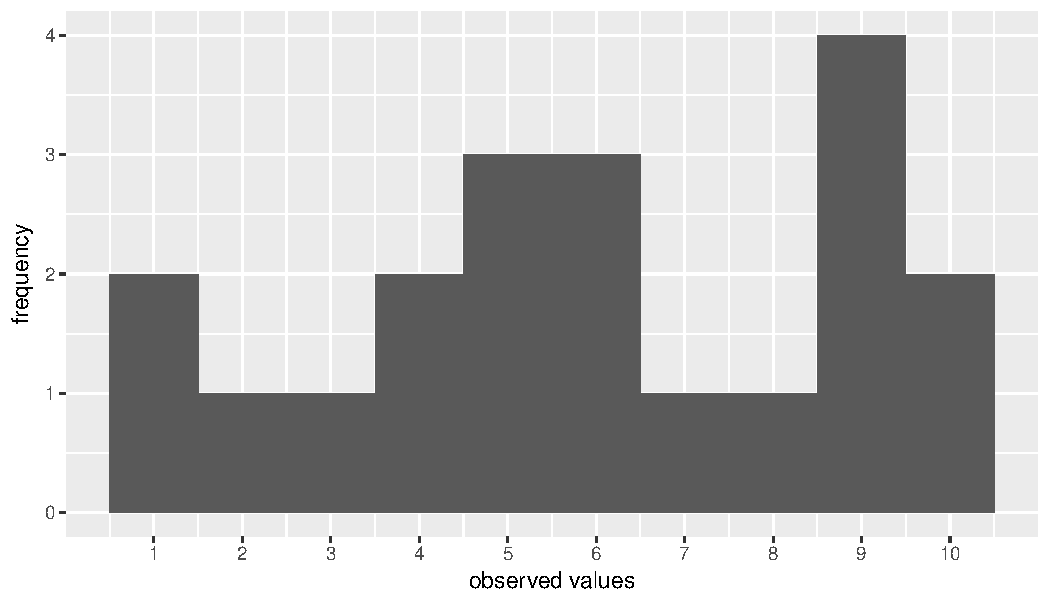
\includegraphics[width=\maxwidth]{figure/distr_1-1} 

}

\caption[A frequency plot]{A frequency plot}\label{fig:distr_1}
\end{figure}


\end{knitrout}

The data in the frequency table can also be represented using a frequency plot. Figure \ref{fig:distr_1} gives the same information, not in numbers but in a graphical way. On the horizontal axis we see several possible values for age in years, and on the vertical axis we see the number of children (the count) that were observed for each particular age. Both the frequency table and the frequency plot tell us something about the \textit{distribution} of age in this imaginary town with 1000 children. For example, both tell us that the oldest child is 17 years old. Furthermore, we see that there are quite a lot of children with ages between 5 and 8, but not so many children with ages below 3 or above 14. The advantage of the table over the graph is that we can get the exact number of children of a particular age very easily. But on the other hand, the graph makes it easier to get a quick idea about the shape of the distribution, which is hard to make out from the table.

% <<distr_1, fig.height=4, echo=FALSE, fig.align='center', message=F, fig.cap='A frequency distribution' >>=
% set.seed(123)
% numbers <- runif(20, 1,10) %>%  round(0)
% data.frame(age) %>%
%         ggplot(aes(numbers)) + geom_bar()  
% +
%         xlab('observed values') + ylab('count')+
%         scale_x_continuous(breaks=seq(1,10))
% @

% Numeric variables have distributions. That means that if you put all the values you observed in order from low to high, you see a certain shape. For example, take the set of following numbers: numbers. If you plot these values on the horizontal axis, and how often they are observed (the \textit{frequency} or \textit{count}) on the vertical you get the frequency plot in Figure \ref{fig:distr_1}. Such a frequency plot is referred to as a \textit{bar chart}.

% Often a \textit{histogram} is plotted. A histogram is very much like a frequency plot or bar chart, except that groups of values can be taken together. Such a group of values is called a \textit{bin}. Figure \ref{fig:distr_2} shows the same data, but uses only 5 bins: for the first bin, we take values of 1 and 2, for the second bin we take values 3 and 4 together, etcetera, until we take vales 9 and 10 for the fifth bin. For each bin, we compute how often we observe the values in that bin. Histograms are also for continous data, for instance if we have values like 3.4, 2,1, etcetera. All values within a bin are defined by their rounded value. For instance, in Figure \ref{fig:distr_2}, all possible values between 2.5 and 4.5 will end up in the second bin. The \textit{binwidth} is here 2: all values between 2.5 and 4.5 are taken to lie in the second bin, and the distance between these values is $4.5-2.5=2$.

Instead of frequency plots, one often see \textit{histograms}. Histograms contain the same information as frequency plots, except that groups of values can be taken together. Such a group of values is called a \textit{bin}. Figure \ref{fig:distr_2} shows the same age data, but uses only 9 bins: for the first bin, we take values of age 0 and 1 together, for the second bin we take ages 2 and 3 together, etcetera, until we take ages 16 and 17 together for the last bin. For each bin, we compute how often we observe the ages in that bin.

Histograms are very convenient for continuous data, for instance if we have values like 3.4, 2,1, etcetera. Or, more generally, for variables with values that have very low frequencies. Suppose that we had measured age not in years but in days. Then we could have had a data set of 1000 children where each and every child had a unique value for age. In that case, the length of the frequency table would be 1000 rows (each value observed only once) and the frequency plot would be very flat. By using age measured in years, what we have actually done is putting all children with an age less than 365 days into the first bin (age 0 years) and the children with an age of at least 365 but less than 730 days into the second bin (age 1 year). And so on. Thus, if you happen to have data with many many values with each of them very low frequencies, consider binning the data, and using a histogram to visualize the distribution of your numeric variable.



\begin{knitrout}
\definecolor{shadecolor}{rgb}{0.969, 0.969, 0.969}\color{fgcolor}\begin{figure}

{\centering 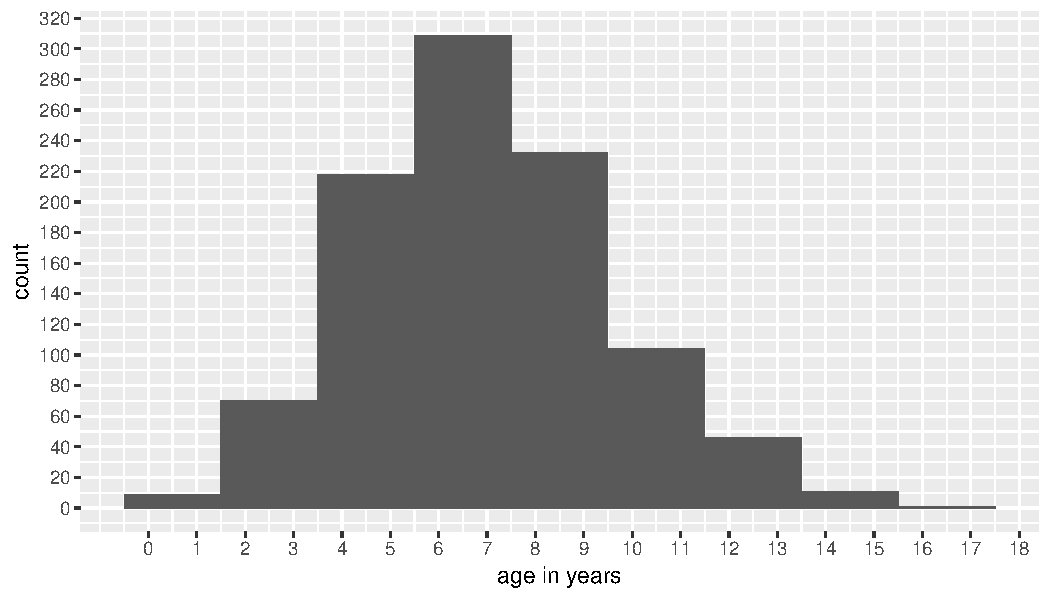
\includegraphics[width=\maxwidth]{figure/distr_2-1} 

}

\caption[A histogram]{A histogram}\label{fig:distr_2}
\end{figure}


\end{knitrout}



\section{Frequencies, proportions and cumulative frequencies and proportions}


When we have for each observed age the frequency, we can calculate the \textit{relative frequency} or \textit{proportion} of children that have that particular age. For example, when we look again at the frequencies in Table \ref{tab:frequency_1} we see that there are two children who have age 0. Given that there are in total 1000 children, we know that the \textit{proportion} of people with age 0 equals $2/1000=0.002$. Thus, the proportion is calculated by taking the frequency and dividing it by the total number of people.


We can also compute \textit{cumulative frequencies}. You get cumulative frequencies by accumulating (summing) frequencies. For instance, the cumulative frequency for the age of 3, is the frequency for age 3 plus all freqencies for younger ages. Thus, the cumulative frequency of age 3 equals 50 + 20 (for age 2) + 7 (for age 1) + 2 (for age 0) = 79. The cumulative frequencies for all ages are presented in Table \ref{tab:frequency_1}.

We can also compute \textit{cumulative proportions}: if we take for each age the proportion of people who have that age \textit{or less}, we get the fifth column in Table \ref{tab:frequency_1}. For example, for age 2, we see that there are 20 children with an age of 2. This corresponds to a proportion of 0.020 of all children. Furthermore, there are 9 children who have an even younger age. The proportion of children with an age of 1 equals 0.007, and the proportion of children with an age of 0 equals 0.002. Therefore, the proportion of all children with an age of 2 or less equals $0.020+0.007+0.002=0.029$, which is called the cumulative proportion for the age of 2.



\section{Quartiles, quantiles and percentiles}

Suppose we want to split the group of 1000 children into 4 equally-sized subgroups, with the 25\% youngest children in the first group, the 25\% oldest children in the last group, and the remaining 50\% of the children in two equally sized middle groups. What ages should we then use to divide the groups? First, we can order the 1000 children on the basis of their age: the youngest first, and the oldest last. We could then use the concept of \textit{quartiles} (from quarter, a fourth) to divide the group in four. In order to break up all ages into 4 subgroups, we need 3 points to make the division, so there are three quartiles. The first quartile is the value below which 25\% of the observations fall, the second quartile is the value below which 50\% of the observations fall, and the third quartile is the value below which 75\% of the observations fall.\footnote{The fourth quartile would be the value below which \textit{all} values are, so that would be the largest value in the row (the age of the last child in the row).}

Let's first look at a smaller but similar problem. For example, suppose your observed values are {10, 5, 6, 21, 11, 1, 7, 9}. You first order them from low to high so that you obtain {1, 5, 6, 7, 9, 10, 11, 21}. You have 8 values, so the first 25\% of your values are the first two. The highest value of these two equals 5, and this we define as our quartile.\footnote{Note that we could also choose to use 6,
because 1 and 5 are lower than 6. Don't worry, the method that we show here to compute quartiles is only one way of doing it. In your life, you might stumble upon alternative ways to determine quartiles. These are just arbitrary agreements made by human beings. They can result in different outcomes when you have small data sets, but usually not when you have large data sets.} We find the second quartile by looking at the values of the first 50\% of the observations, so 4 values. The first 4 values are 1, 5, 6, and 7. The last of these is 7, so that is our second quartile. The first 75\% of the observations are 1, 5 ,6 ,7 , 9, and 10. The value last in line is 10, so our fourth quartile is 10.

The quartiles as defined here can also be found graphically, using cumulative proportions. Figure \ref{fig:quartile_1} shows for each observed value the cumulative proportion. It also shows where the cumulative proportions are equal to 0.25, 0.50 and 0.75. We see that the 0.25 line intersects the other line at the value of 5. This is the first quartile. The 0.50 line intersects the other line at a value of 7, and the 0.75 line intersects at a value of 10. The three percentiles are therefore 5, 7 and 10.


\begin{figure}

{\centering 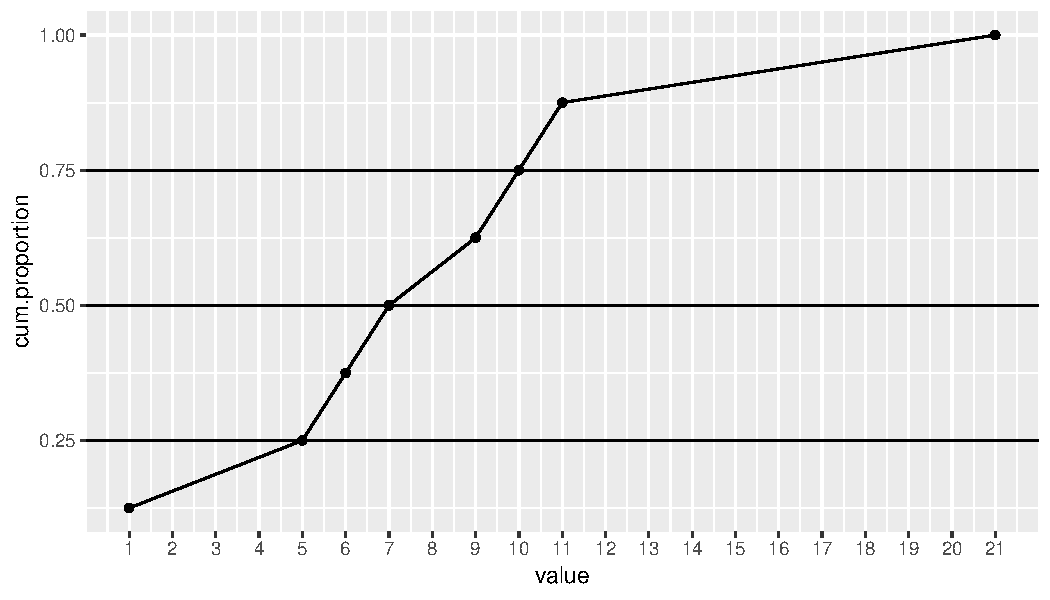
\includegraphics[width=\maxwidth]{figure/quartile_1-1} 

}

\caption[Cumulative proportions]{Cumulative proportions.}\label{fig:quartile_1}
\end{figure}



The graphical way is far easier for large data sets. If we plot the cumulative proportions for the ages of the 1000 children, we obtain Figure \ref{fig:quartile_2}. We see a nice S-shaped curve. We also see that the three horizontal quartile lines no longer intersect the curve at specific values, so we need a rule to determine what value to pick. By eyeballing we can find that the first quartile is somewhere between 4 and 5. This tell us that the youngest 25\% of children have ages of 5 or less\footnote{If you don't see that, read again the section on cumulative proportions and how they are computed.}. The second quartile is somewhere between 6 an 7, so we know that 50\% of the youngest children is 7 years old or younger The third quartile is somewhere between 8 and 9 and this tells us that the youngest 75\% of the children is age 9 or younger Thus, we can call 5, 7 and 9 our three quartiles.



\begin{figure}

{\centering 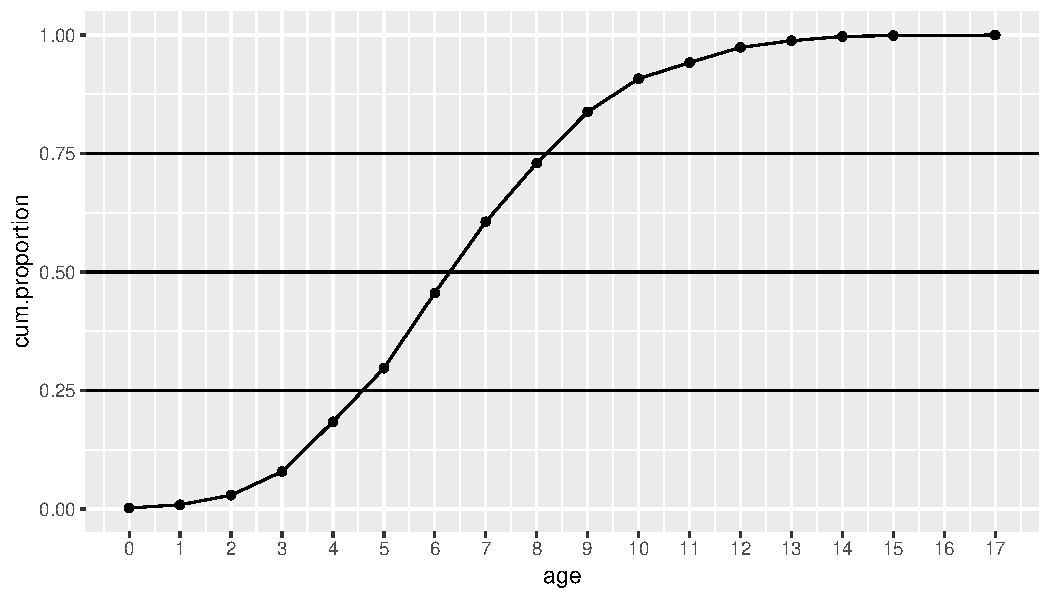
\includegraphics[width=\maxwidth]{figure/quartile_2-1} 

}

\caption[Cumulative proportions]{Cumulative proportions.}\label{fig:quartile_2}
\end{figure}




Alternatively, we could also use the frequency table (Table \ref{tab:frequency_1}). First, if we want to have 25\% of the children that are the youngest, and we know that we have 1000 children in total, we should have $0.25 * 1000=250$ children in the first group. So if were to put all the children in a row, ordered from youngest to oldest, we want to know the age of the 250th child.

In order to find the age of this 250th child, and we look at Table \ref{tab:frequency_1}, we see that 29.7 \% of the children have an age of 5 or less (297 children), and 18.4 \% of the children have an age of 4 or less (184 children). This tells us that the 250th child must be 5 years old. Furthermore, if we want to find a cut-off age for the oldest 25\%, we see from the table, that 83.8\% of the children (838 children) have an age of 9 or less, and 73.0\% of the children (730) have an age of 8 or less. Therefore, the age of the 750th child (when ordered from youngest to oldest) must be 9.


What we just did for quartiles, (i.e. 0.25, 0.50, 0.75) we can do for any proportion between 0 and 1. We then no longer call them quartiles, but \textit{quantiles}. A quantile is the value below which a given proportion of observations in a group of observations fall. From this table it is easy to see that a proportion of 0.606 of the children have an age of 7 or less. Thus, the 0.606 quantile is 7. One often also sees \textit{percentiles}. Percentiles are very much like quantiles, except that they refer to percentages rather than proportions. Thus, the 20th percentile is the same as the 0.20 quantile. And the 0.81 quantile is the same as the 81st percentile.

The reason that quartiles, quantiles and percentiles are important is that they are very short ways of saying something about a distribution. Remember that the best way to represent a distribution is either a frequency table or a frequency plot. However, since they can take up quite a lot of space sometimes, one needs other ways to briefly summarize a distribution. Saying that "the third quartile is 454" is a condensed way of saying that "75\% of the values is either 454 or lower". In the next sections, we look at other ways of summarizing information about distributions.

\subsection{Exercises}

% latex table generated in R 3.5.0 by xtable 1.8-2 package
% Mon Jan 21 16:42:03 2019
\begin{table}[ht]
\centering
\caption{Freqency table for x, with proportions and cumulative proportions.} 
\label{tab:frequency_2}
\begin{tabular}{rrrr}
  \hline
x & frequency & proportion & cum.proportion \\ 
  \hline
   0 &    6 & 0.030 & 0.030 \\ 
     1 &   25 & 0.125 & 0.155 \\ 
     2 &   55 & 0.275 & 0.430 \\ 
     3 &   44 & 0.220 & 0.650 \\ 
     4 &   36 & 0.180 & 0.830 \\ 
     5 &   20 & 0.100 & 0.930 \\ 
     6 &    9 & 0.045 & 0.975 \\ 
     7 &    4 & 0.020 & 0.995 \\ 
     8 &    1 & 0.005 & 1.000 \\ 
   \hline
\end{tabular}
\end{table}


\begin{enumerate}
\item Look at Table \ref{tab:frequency_2}. Determine the 10th quantile for variable \textbf{x}.

\item Determine the 95th percentile.

\item Determine the first quartile.

\item Determine the second quartile.

\item Determine the 50th percentile.

\item Determine the third quantile.

\item Determine the 0.75 quantile.

\item Suppose we have the values {6,5,4,8,6,5,6,4,5,6,7,8}. Determine the third quartile.

\item Suppose we have the values {4,4,4,8,6,4,6,4,5,6,7,8}. Determine the third quartile.

\item From Figure \ref{fig:quartile_3}, determine the 30th, 40th and 90th percentiles.

\begin{figure}

{\centering 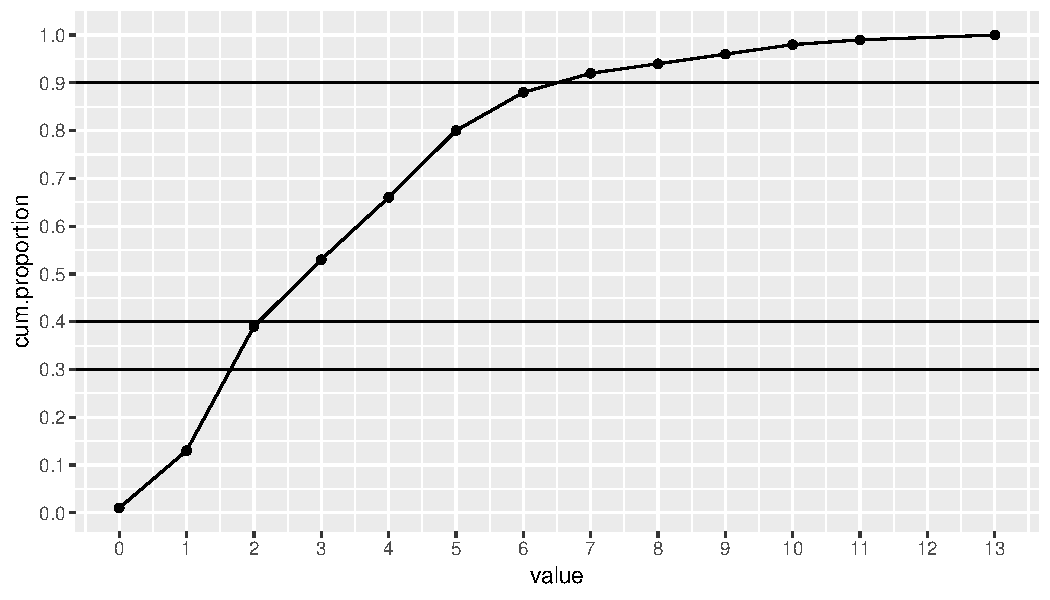
\includegraphics[width=\maxwidth]{figure/quartile_3-1} 

}

\caption[Cumulative proportions]{Cumulative proportions.}\label{fig:quartile_3}
\end{figure}



\item Suppose yesterday you did an IQ test, together with 999 other students. Today you hear that you scored 100 points. They tell you that the 8th percentile was a score of 80, and the 9th percentile was a score of 100. What does that tell you about your performance yesterday?


\end{enumerate}


\subsection{Answers}

\begin{enumerate}

\item
1
\item
6
\item
2
\item
3
\item
3
\item
4
\item
4
\item
ordered series: 445 556 666 788, last value of third quart: 6
\item
orderd series: 444 445 666 788, last value of third quart: 6

\item
2, 2 and 7

\item

Nine percent of my fellow students scored the same or lower than I did on the exam, so 91 percent did better. I did not do so well.

\end{enumerate}






\section{Measures of central tendency}

The mean, the median and the mode are three different measures that say something about the \textit{central tendency} of a distribution. If you have a series of values: around which value do they tend they tend to cluster?

\subsection{The mean}
Suppose we have the values 1, 2 and 3, then we compute the mean (or average) by first adding these numbers and then divide them by the number of values we have. In this case we have three values, so the mean is equal to $(1 + 2 + 3)/3 = 2$. In statistical formulas, the mean is indicated by a bar above the variable. So if our values of variable $y$ are 1, 2 and 3, then we denote the mean by $\bar{y}$ (pronounced as y-bar). For taking the sum of a set of values, statistical formulas show a $\Sigma$ (pronounced as sigma). So we often see the following formula for the mean of a set of $n$ values for variable $y$:

\begin{equation}
\bar{y} = \frac{\Sigma_i^n y_i}{n}
\end{equation}

In words, we take every value for $y$ from 1 to $n$ and sum them, and the result is divided by $n$.

If we take another example, suppose we have variable $y$ with the values {6, -3, and 21}, then the mean of $y$, $\bar{y}$, equals:

\begin{equation}
\bar{y} = \frac {  \Sigma y_i^n} {n} =    \frac{y_1 + y_2 + y_3}{n} = \frac{6 + (-3) + 21}{3} = \frac{24}{3} = 8
\end{equation}







\subsection{The median}
The mean is only one measure of central tendency: if the mean is 100, it says that the values tend to cluster around this value. A different measure of central tendency is the median. The median is nothing but the middle value of an ordered series. Suppose we have the values 45, 567, and 23. Then what value lies in the middle? Let's first order them from small to large to get a better look, then we get 23, 45 and 567. Then the value in the middle is of course 45.

Suppose we have the values 45, 45, 45, 65, and 23. What is the middle value? We first order them again and see what value is in the middle: 23, 45, 45, 45 and 65. Obviously now 45 is the median. You can also see that half of the values is equal or smaller than this value, and half of the values is equal or larger than this value. The median therefore is the same as the second quartile.

What if we have two values in the middle? Suppose we have the values 46, 56, 45 and 34. If we order them we get 34, 45, 46 and 56. Now there are two values in the middle: 45 and 46. In that case, we take the mean of these two middle values, so the median is 45.5. 

When do you use a median and when do you use a mean? For numeric variables that have a more or less symmetric distribution (i.e., a frequency plot that is more or less symmetric), the mean is best used. For numeric variables that do not have a symmetric distribution, it is usually more informative to use the median. An example of such a situation is income. Figure \ref{fig:median} shows a typical distribution of yearly income. The distribution is highly asymmetric, it is severely skewed to the right. The bulk of the values are between 20,000 and 40,000, with only a very few extreme values on the high end. Even though there are only a few people with a very high income, the few high values have a huge effect on the mean.

\begin{figure}

{\centering 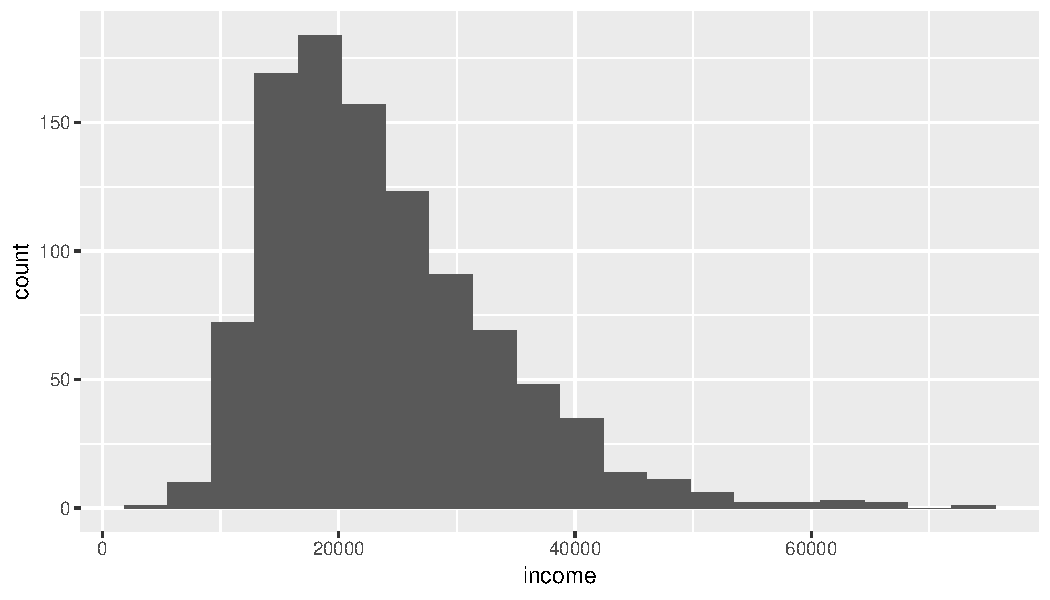
\includegraphics[width=\maxwidth]{figure/median-1} 

}

\caption[Distribution of yearly income]{Distribution of yearly income.}\label{fig:median}
\end{figure}



The mean of the distribution turns out to be 23604. The largest value in the distribution is an income of 75051. Imagine what would happen to the mean and the median if we would change only this one value. Which would be most affected, do you think: the mean or the median?



Well, if we would change this value into 85051, you see an immediate impact on the mean: the mean is then 23614. This means that the mean is very sensitive to extreme values. One single change in a data set can have a huge effect on the mean. The median on the other hand is much more stable. The median remains unaffected by slight changes in the extremes. This because it only looks at the middle value. The middle value is unaffected by a change in the extreme values, as long as the order of the values remains the same.

This might be even made more clear by the following example in Table \ref{tab:median_2}. Suppose we have the values 4, 5, and 8. Obviously, the median is 5. Instead of 8, we could pick 80, or 800, or 8000. Regardless, the middle value of this series remains 5. In contrast, the mean would be very much affected by having either an 8, a 80, a 800 or an 8000 in the series. In sum: the median is a more stable measure of central tendency than the mean.


% latex table generated in R 3.5.0 by xtable 1.8-2 package
% Mon Jan 21 16:42:04 2019
\begin{table}[ht]
\centering
\caption{Four series of values and their respective medians and means.} 
\label{tab:median_2}
\begin{tabular}{rrrrr}
  \hline
X1 & X2 & X3 & median & mean \\ 
  \hline
4 & 5 & 8 & 5 & 5.7 \\ 
  4 & 5 & 80 & 5 & 29.7 \\ 
  4 & 5 & 800 & 5 & 269.7 \\ 
  4 & 5 & 8000 & 5 & 2669.7 \\ 
   \hline
\end{tabular}
\end{table}




\subsection{The mode}
A third measure of central tendency is the \textit{mode}. The mode is defined as the value that we see most frequently in a series of values. For example, if we have the series 4, 7, 5, 5, 6, 6, 6, 4, then the value observed most often is 6 (three times). Modes are easily inferred from frequency tables: the value with the largest frequency is the mode. They are also easily inferred from frequency plots: the value on the horizontal axis for which we see the highest count (on the vertical axis).

The mode can also be determined for categorical variables. If we have the observed values  'Dutch', 'Danish', 'Dutch', and 'Chinese', the mode is 'Dutch' because that is the value that is observed most often.

If we look back at the distribution in Figure \ref{fig:median}, we see that the peak of the distribution is around the value of 19,000. However, whether this is the mode, we cannot say. Because income is a more or less continuous variable, every value observed in the Figure occurs only once: there is no value of income with a frequency more than 1. So technically, there is no mode. However, if we split the values into 20 bins, like we did for the histogram in Figure \ref{fig:median}, we see that the fifth bin has the highest frequency. In this bin there are values between 17000 and 21000, so our mode could be around there. If we really want a specific value, we could decide to taken the average value in the fifth bin. There are many other statistical tricks to find a value for the mode, where technically there is none. The point is that for the mode, we're looking for the value or the range of values that are most frequent. Graphically, it is the value under the peak of the distribution. Similar to the median, the mode is also quite stable: it is not much affected by extreme values and is therefore to be preferred over the mean in the case of assymetric distributions.



\subsection{Exercises}

\begin{enumerate}

\item If we have values 56, 78, 23 and 45, what is the mean?

\item If we have values 56, 78, 23 and 45, what is the median?

\item If we have values 56, 23, 78, 23 and 45, what is the mode?

\item Figure \ref{fig:mode} shows a distribution of systolic bloodpressure measures in older men. What would be more or less the mode of these values?

\begin{figure}

{\centering 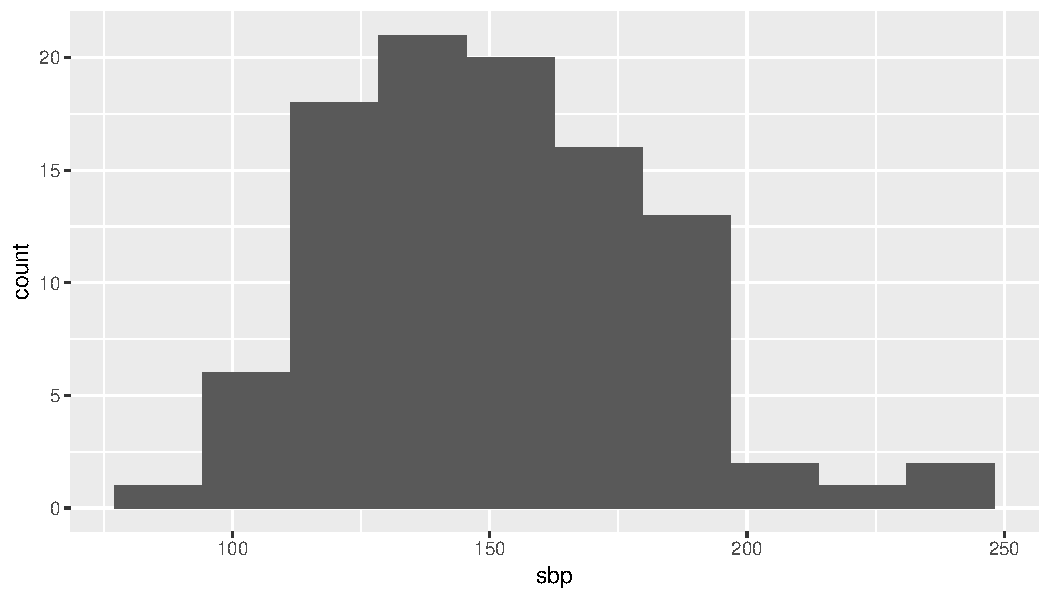
\includegraphics[width=\maxwidth]{figure/mode-1} 

}

\caption[Distribution of systolic bloodpressure]{Distribution of systolic bloodpressure.}\label{fig:mode}
\end{figure}



\item Figure \ref{fig:quartile_3} shows a distribution of values. What would be more or less the median of these values?

\item Figure \ref{fig:mode2} shows a distribution of number of bicycles for 100 households. If you could choose only one statistic to describe this distribution, what would you choose to report: the mean, the mode or the median? Motivate your answer.

\begin{figure}

{\centering 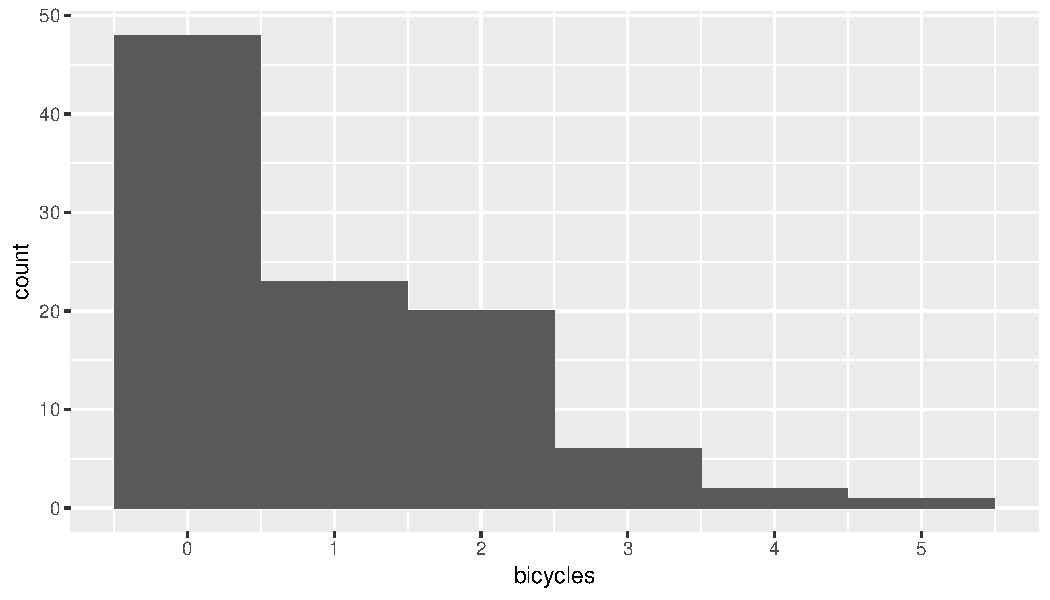
\includegraphics[width=\maxwidth]{figure/mode2-1} 

}

\caption[Distribution of systolic bloodpressure]{Distribution of systolic bloodpressure.}\label{fig:mode2}
\end{figure}





\end{enumerate}


\subsection{Answers}

\begin{enumerate}
\item 50.5
\item 50.5
\item  23
\item 140
\item 3
\item The median. Because the distribution is very skew and in that case the mean would be relatively high, because it is influenced by a few households with very many bicycles. The mode would not say very much other than that 0 bicycles is the most common observation. But saying that half the households have at least 1 bicycle would be more informative than that. 

\end{enumerate}


\section{Relationship between measures of tendency and measurement level}

There is a close relationship between measures of tendency and measurement level. For numeric variables, all three measures of tendency are meaningful. Suppose you have the numeric variable age measured in years, with the values 56, 68, 68, 99 and 100. Then it is meaningful to say that the average age is 78.2 years, that the median age is 68 years, and that the mode is 68 years.

For ordinal variables, it is quite different. Suppose you have 5 T-shirts, with the following sizes: M, S, M, L, XL. Then what is the average size? There are no numeric values here to put in the algebraic formula. But we can determine the median: if we order the values from small to large we get the set S, M, M, L, XL and we see that the middle value is M. So M is our median in this case. \footnote{However, suppose that our collection of T-shirts had the following sizes: S, M, L, L. Then there would be no single middle value in we would have to average the M and L values, which would be impossible!} The other meaningful of tendency for ordinal variables is the mode.

For categorical variables, both the mean and the median are pointless to report. Suppose we have the nominal variable Study Programme with observed values "Medicine", "Engineering", "Engineering", "Mathematics", and "Biology". It would be impossible to derive a numerical mean, nor would it be possible to determine the middle value to determine the median, as there is no logical or natural order. \footnote{Unless you see one? But then it would not be a categorical value but an ordinal variable.} It is meaningful though to report a mode. It would be meaningful to state that the study programme mentioned most often in the news is "Psychology", or that the most popular study program in India is "Engineering". Thus, for categorical variables, both dichotomous and nominal variables, only the mode is a meaningful measure of central tendency.

As stated earlier, the appearance of a variable in a data matrix can be quite misleading. Categorical variables and ordinal variables can often look like numeric variables, which makes it very tempting to compute means and medians where they are completely meaningless. Take a look at Table \ref{tab:modemedian}. It is entirely possible to compute the average University, Size, or Programme, but it would be utterly senseless to report these values.

It is entirely possible to compute the median University, Size, or Programme, but it is only meaningful to report the median for the variable Size, as Size is an ordinal value. Reporting that the median size is equal to 2 is saying that about half of the study programs is of medium size or small, and about half of the study programs is of medium size or large.

It is entirely possible to compute the mode for the variables University, Size, or Programme, and it is always meaningful to report them. It is meaningful to say that in your data there is no University that is observed more than others. It is meaningful to report that most study programmes are of medium size, and that most study programmes are study programme number 2 (don't forget to look up and write down which study programme that actually is!).



% latex table generated in R 3.5.0 by xtable 1.8-2 package
% Mon Jan 21 16:42:04 2019
\begin{table}[ht]
\centering
\caption{Study programs and their relative sizes (1=small, 2=medium, 3=large) for six different universities.} 
\label{tab:modemedian}
\begin{tabular}{rrr}
  \hline
University & Size & Programme \\ 
  \hline
1 & 1 & 2 \\ 
  2 & 3 & 2 \\ 
  3 & 2 & 3 \\ 
  4 & 2 & 3 \\ 
  5 & 3 & 4 \\ 
  6 & 2 & 1 \\ 
   \hline
\end{tabular}
\end{table}





\section{Measures of variation}

Above we have seen that we can summarize a distribution of numeric variable by a measure of central tendency. Here we discuss how we can summarize a distribution of a numeric variable by a measure that describes its \textit{variation}.

Suppose we measure the height of 3 children, and their heights (in cms) are 120, 120 and 120. There is no variation in height: all heights are the same. There are no differences. Then the average height is 120, the median height is 120, and the mode is 120.

Now suppose their heights are . Now there are differences: one child is taller than the other two, who have the same height. There is some variation now. We know how to quantify the mean, which is 125, we know how to quantify the median, which is 120, and we know how to quantify the mode, which is also 120. But how do we quantify the variation? Is there a lot of variation, or just a little, and how do we measure it?

\subsection{Range and interquartile distance}

One thing you could think of is measuring the distance or difference between the lowest value and the highest value. This we call the \textit{range}. The lowest value is 120, and the highest value is 135, so the range of the data is equal to $135-120=15$. As another example, suppose we have the values 20, 20, 21, 20, 19, 20 and 454. Then the range is equal to $454-19=435$. That's a large range, for a series of values that for the most part hardly differ from another.

Instead of measuring the distance from the lowest to the highest value, we could also measure the distance between the first and the third quartile: how much does the first quartile \textit{deviate} from the third quartile? This distance or deviation is called the \textit{interquartile distance}. Suppose that we have a large number of systolic bloodpressure measurements, where 25\% are 120 or lower, and 75\% are 147 or lower, then the interquartile distance is equal to $147-120=27$.

Thus, we can measure variation using the range or the interquartile distance. A third measure for variation is \textit{variance}, and variance is based on the \textit{sum of squares}.

\subsection{Sum of squares}

What we call a sum of squares is actually a sum of squared deviations. But deviations from what? We could for instance be interested in how much the values 120, 120, 135 vary around the mean of these values. The mean of these three values equals 125. The first value differs $120-125= -5$, the second value also differs $120-125= -5$, and the third value differs $135-125= 10$.

Always when we look at deviations from the mean, some deviations are positive and some deviations will be negative (except when there is no variation). If we want to measure variation, it should not matter whether deviations are positive or negative: any deviation should add to the total variation in a positive way. Moreover, if we would add up all deviations from the mean, we would always end up with 0. So that is why we should better make all deviations positive, and this can be done by taking the square of the deviations. So for our three values 120, 120 and 135, we get the deviations -5, -5 and +10, and if we square these deviations, we get 25, 25 and 100. If we add these three squares, we obtain the 150.

In most cases, the sum of squares (SS) refers to the sum of squared deviations from the mean. In brief, suppose you have $n$ values of a variable $y$, you first take the mean of those values (this is $\bar{y}$), you subtract this mean from each of these $n$ values ($y-\bar{y}$), then you take the squares of these deviations ($(y-\bar{y})^2$), and then add them toghether (take the sum of these squared deviations, $\Sigma (y-\bar{y})^2)$. In formula form, this process looks like:

\begin{equation}
SS = \Sigma_i^n (y_i-\bar{y})^2
\end{equation}

As an example, suppose you have the values 10, 11 and 12, then the mean is 11. Then the deviations from the mean are -1, 0 and +1. If you square them you get $(-1)^2=1$, $0^2=0$ and $(+1)^2=1$, and if you add these three values, you get $SS=1+0+1=2$. In formula form:


\begin{eqnarray}
SS &=& (y_1-\bar{y})^2 + (y_2-\bar{y})^2 +(y_3-\bar{y})^2 \\
&=& (10-11)^2 + (11-11)^2 +(12-11)^2 = (-1)^2 + 0^2 + 1^2=2 \nonumber
\end{eqnarray}

Now let's use some values that are more different from eachother, but with the same mean. Suppose you have the values 9, 11 and 13. The average value is still 11, but the deviations from the mean are larger. The deviations from 11 are -2, 0 and +2. Taking the squares, you get $(-2)^2=4$, $0^2=0$ and $(+2)^2=4$ and if you add them you get $SS=4+0+4=8$.

\begin{eqnarray}
SS &=& (y_1-\bar{y})^2 + (y_2-\bar{y})^2 +(y_3-\bar{y})^2 \\
&=& (9-11)^2 + (11-11)^2 +(13-11)^2= (-2)^2 + 0^2 + 2^2=8 \nonumber
\end{eqnarray}

Thus, the more values differ from eachother, the larger the deviations from the mean. And the larger the deviations from the mean, the larger the sum of squares. The sum of squares is therefore a nice measure of how much values differ from eachother.

\subsection{Variance and standard deviation} \label{sec:standarddeviation}

The sum of squares can be seen as some kind of total variation: all deviations from a certain value are added up. This means that the more data values you have, the larger the sums of squares. Oftentimes, you are not interested in the total variation, but you're interesed in the average variation. Suppose we have the values 10, 11 and 24. The mean is then $45/3=15$. We have two values that are smaller than the average and one value that is larger than the average, so two negative deviations and one positive deviation. Squaring them makes them all positive. The squared deviations are 25, 16, and 81. The third value has a huge squared deviation (81) compared to the other two values. If we take the \textit{average} squared deviation, we get $(25+16+81)/3 \approx 40.67$. So the average squared deviation is equal to 40.7. This value we call the \textit{variance}. So the variance of a bunch of values is nothing but the $SS$ divided by the number of values, $n$. The variance is \textit{the average squared deviation from the mean}. The symbol used for the variance is usually $\sigma^2$ (pronounced as "sigma squared").

\begin{equation}
\sigma^2 = \frac{SS}{n}= \frac{\Sigma_i^n (y_i-\bar{y})}{n}
\end{equation}


As an example, suppose you have the values 10, 11 and 12, then the average value is 11. Then the deviations are -1, 0 and 1. If you square them you get $(-1)^2=1$, $0^2=0$ and $1^2=1$, and if you add these three values, you get $SS=1+0+1=2$. If you divide this by 3, you get the variance: $\frac{2}{3}$. Put differently, if the squared deviations are 1, 0 and 1, then the average squared deviation (i.e., the variance) is $\frac{1+0+1}{3}=\frac{2}{3}$.

As another example, suppose you have the values 8, 10, 10 and 12, then the average value is 10. Then the deviations from 10 are -2, 0, 0 and +2. Taking the squares, you get 4, 0, 0 and 4 and if you add them you get $SS=8$. To get the variance, you divide this by 4: $8/4=2$. Put differently, if the squared deviations are 4, 0, 0 and 4, then the average squared deviation (i.e., the variance) is $\frac{4+0+0+4}{4}=2$.

Often we also see another measure of variation: the \textit{standard deviation}. The standard deviation is the squared root of the variance and is therefore denoted as $\sigma$:

\begin{equation}
\sigma = \sqrt{\sigma^2}=\sqrt{  \frac{\Sigma_i^n (y_i-\bar{y})}{n}}
\end{equation}

The standard deviation is often used to indicate how deviant a particular value is from the rest of the values. Take for instance an IQ score of 105. Is that a high IQ score or a low IQ score? Well, if someone tells you that the average person has an IQ score of 100, you know that a score of 105 is above avarage. However, still you do not know whether it is much higher than average, or just slightly higher than average. Suppose I tell you that the standard deviation of IQ scores is 15, then you know that a score of 105 is a third of standard deviation above the mean. Therefore, in order to know how deviant a particular value is relative to a the rest of the values, one needs both a measure of central tendency and a measure of variation. In psychological testing, IQ testing for instance, one usually uses the mean and the standard deviation to express someone's score as the number of standard deviations above or below the average score. This process of counting the number of standard deviations is called \textit{standardization}. If we go back to the IQ score of 105, and if we want to standardize the score in terms of standard deviations from the mean, we saw that a score of 105 was a third of a standard deviation above the mean, so $+\frac{1}{3}$. As another example, suppose the mean is 100 and we observe an IQ score of 80, we see that we are $80-100=20$ points below the average of 100. This is equal to $20/15=5/4$ standard deviations below the average, so our standardized measure equals $-5/4$.



\subsection{Exercises}

\begin{enumerate}
\item Suppose we have the values 9, 6, 5, and 66. What is the range?
\item Suppose we have the values -9, 6, -5, and 66. What is the range?
\item Suppose we have the values 9, 6, 5, and 4. What is the sum of squared deviations from 0?
\item Suppose we have the values 9, 6, 5, and 4. What is the sum of squared deviations from the mean?
\item Suppose we have the values -7, 6, -5, and 6. What is the sum of squared deviations from the mean?
\item Suppose we have the values -7, 6, -5, and 6. What is the variance?
\item Suppose we have the values 77, 76, and 78. What is the standard deviation?
\item Suppose we have the values 197, 197, and 197. What is the standard deviation?
\end{enumerate}

Answers:


\begin{enumerate}
\item Smallest value is 5, largest value is 66. The range is $66-5=61$.
\item Smallest value is -9, largest value is 66. The range is $66-(-9)=75$.
\item $9^2+6^2+5^2+4^2=81+36+25+16=158$
\item The mean is $(9+6+5+4)/4=6$. So we have $(9-6)^2+(6-6)^2+(5-6)^2+(4-6)^2=9+0+1+4=14$.
\item The mean is $(-7+6-5+6)/4=0$. So we have $(-7)^2+6^2+(-5)^2+6^2=49+36+25+36=146$.
\item The mean is 0. So the sums of squares equals $(-7)^2+6^2+(-5)^2+6^2=49+36+25+36=146$. Then the variance is $146/4=36.5$.
\item The average is $(77+76+78)/3=77$. The sum of squares is then $(-1)^2+0^2+1^2=2$. The variance is then $2/3=0.67$. The standard deviation is the root of the variance, so $\sqrt{0.67}=0.82$.
\item All values are the same: there is no variation. Therefore the variance is 0, and therefore the standard deviation is $\sqrt{0}=0$.
\end{enumerate}



\section{Density plots}

Earlier in this chapter we saw that when we have a certain number of values for a numeric variable, frequency tables and frequency plots fully describe all values of the variable that are observed. A histogram is a helpful tool to visualize the distribution of a variable when there so many different values that a frequency table would be too long and a frequency plot would become too cluttered. 

% Another helpful tool to summarize a distribution is a measure of central tendency. A measure of central tendency describes very succcintly where values of the variable tend to cluster. A measure of spread or variation describes how much variation there is around such a meusure of central tendency. For instance, the variance very succintly describes how much variation there is around the mean of the distribution.  

A histogram can then be used to give a quick graphical overview of the distribution. The binwidth is usually chosen rather arbitrarily. Figure \ref{fig:histbin1} shows a histogram of one million values of a numeric variable, say yearly \textbf{wage} for an administrative clerk. Figure \ref{fig:histbin2} shows a histogram for the exact same data, but now using a much smaller bin size. You see that when you have a lot of values, a million in this case, you can choose a very small bin size, and in some cases this can result in a very clear shape of the distribution.

\begin{knitrout}
\definecolor{shadecolor}{rgb}{0.969, 0.969, 0.969}\color{fgcolor}\begin{figure}

{\centering 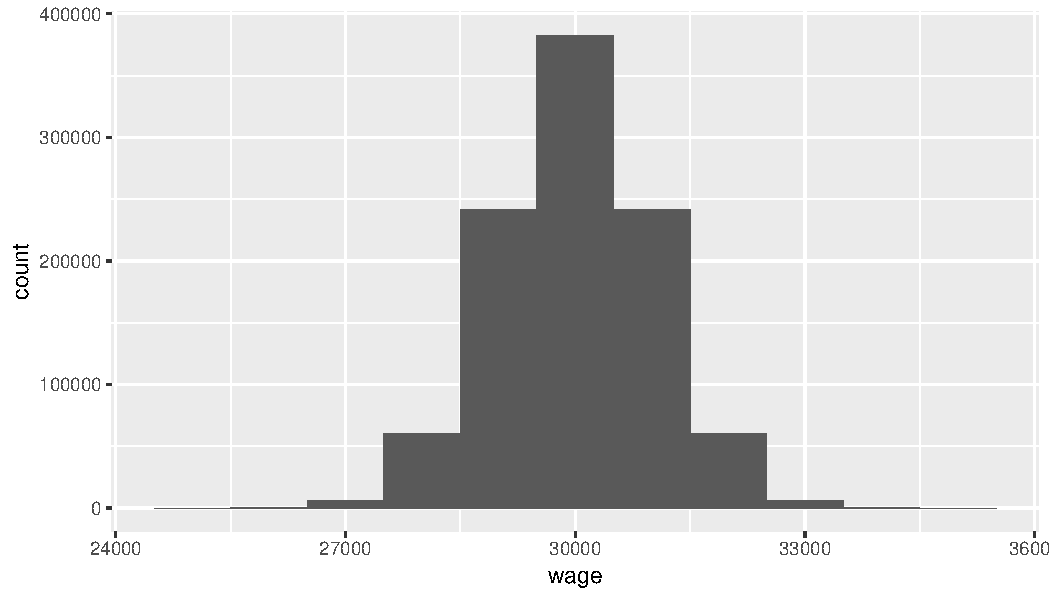
\includegraphics[width=\maxwidth]{figure/histbin1-1} 

}

\caption[A histogram of wages with bin size 1000]{A histogram of wages with bin size 1000.}\label{fig:histbin1}
\end{figure}


\end{knitrout}

\begin{knitrout}
\definecolor{shadecolor}{rgb}{0.969, 0.969, 0.969}\color{fgcolor}\begin{figure}

{\centering 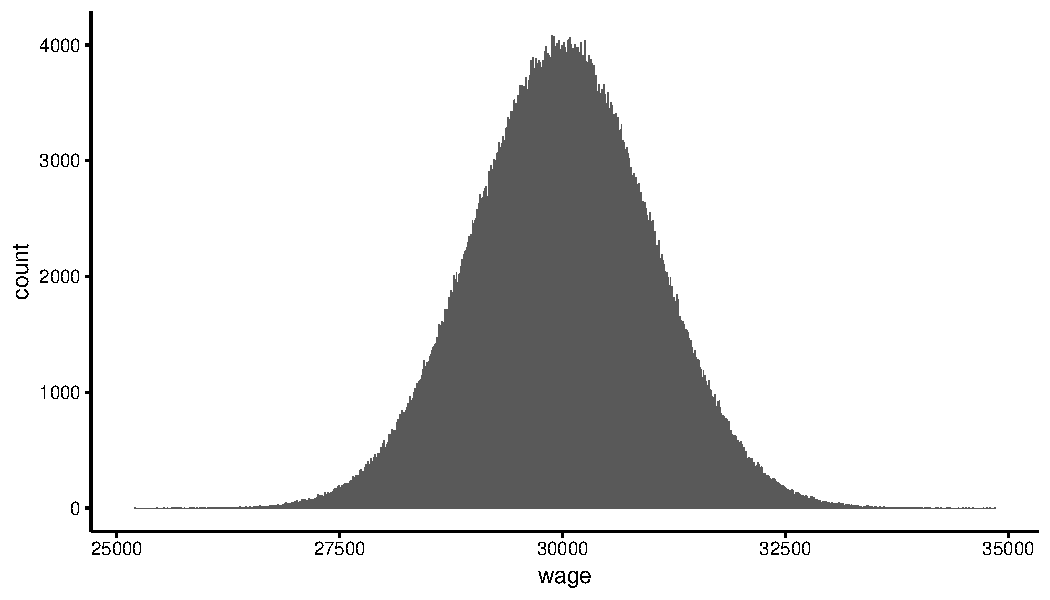
\includegraphics[width=\maxwidth]{figure/histbin2-1} 

}

\caption[A histogram of wages with bin size 10]{A histogram of wages with bin size 10.}\label{fig:histbin2}
\end{figure}


\end{knitrout}

The shape of the distribution that we discern in Figure \ref{fig:histbin2} can be represented by a \textit{density plot}. Density plots are an elegant representation of how the frequency of certain values are distributed across a continuum. They are particularly suited for large amounts of non-discrete (continuous) values, typically more than 1000. Figure \ref{fig:densitywages} shows a density plot of the one million wages. They more or less 'smooth' the histogram: drawing a smooth line connecting the dots of the histogram in Figure \ref{fig:histbin2} while looking through your eyelashes. On the vertical axis, we no longer see 'count' or 'frequency', but 'density'. The quantity \textit{density} is defined such that the area under the curve equals 1. Density plots are particularly suited for large data sets, where one is no longer interested in the particular counts, but  more interested in relative frequencies: how often are certain values observed, relative to other values. From this density plot, it is very clear that, relatively speaking, there are more values between around 30,000 than around 27,500 or 32,500.

\begin{knitrout}
\definecolor{shadecolor}{rgb}{0.969, 0.969, 0.969}\color{fgcolor}\begin{figure}

{\centering 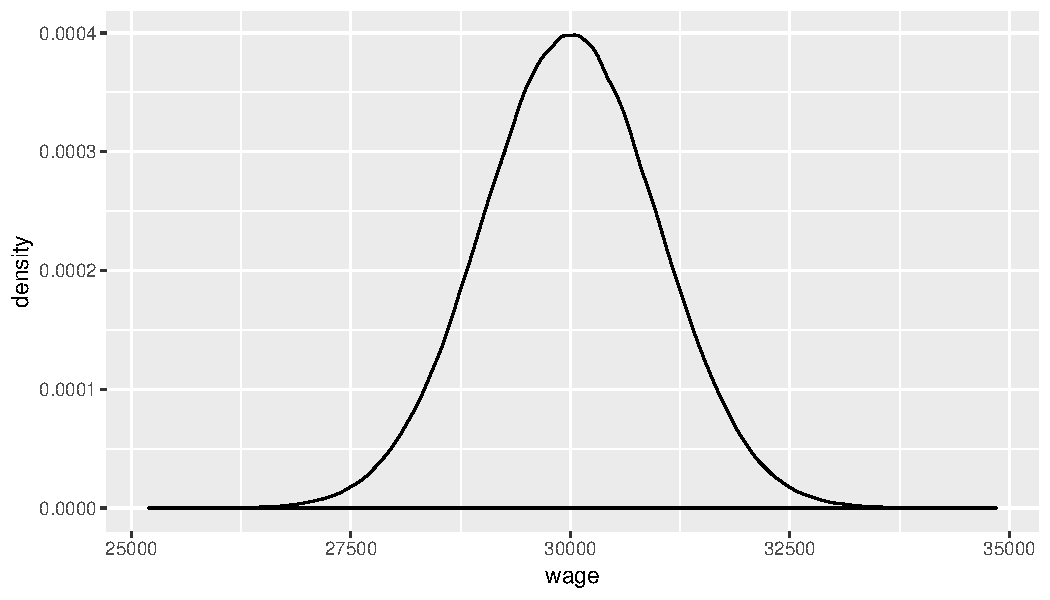
\includegraphics[width=\maxwidth]{figure/densitywages-1} 

}

\caption[A histogram of wages with bin size 10]{A histogram of wages with bin size 10.}\label{fig:densitywages}
\end{figure}


\end{knitrout}





% Figure \ref{fig:distr_3} shows a density plot of 1000 temperature values between 50 and 60 Fahrenheit, where all values had a precision of 4 decimal points (i.e., values like 53.9845, 56.0912, etc.). The plot suggests that values around 55 degrees are most frequent, and that values around 52 or around 58 are rather infrequent in the data set. On the vertical axis, we no longer see 'count' or 'frequency', but we see 'density'. Density is defined such that the area under the curve equals 1. Density plots are particularly suited for large data sets, where one is no longer interested in the particular counts: we're more interested in relative frequencies: how often are certain values observed, relative to other values. From this density plot, it is very clear that, relatively speaking, there are more values between 54 and 55 than between 52 and 53.
% 
% <<distr_3, fig.height=4, echo=FALSE, fig.align='center', message=F,warning=FALSE, fig.cap='Density plot of 1000 observed temperature measures.' >>=
% set.seed(1234)
%  data_frame(temperature = rnorm(1000,55, 1)) %>%
%         ggplot(aes(temperature)) + geom_density()  +
%         scale_x_continuous(breaks=seq(50, 60)) +
%         xlim(c(50,60))
% @




\section{The normal distribution}

Sometimes distributions of observed variables bear close resemblance to \textit{theoretical} distributions. For instance, Figure \ref{fig:densitywages} bears close resemblance to the theoretical \textit{normal} distribution with mean 30,000 and standard deviation 1000. This theoretical shape can be described with the mathematical function

\begin{equation}
f(x)  = \frac{1}{\sqrt{2 \pi 1000^2}} e^{ { -\frac{(x - 30000)^2}{2 \times  1000^2}  } }
\end{equation}

which you are allowed to forget immediately. It is only to illustrate that distributions observed in the wild (empirical distributions) sometimes resemble  mathematical functions (theoretical distributions).

The density function of that distribution is plotted in Figure \ref{fig:distr_4}. Because of its bell-shaped form, the normal distribution is sometimes informally called 'the bell curve'.




\begin{knitrout}
\definecolor{shadecolor}{rgb}{0.969, 0.969, 0.969}\color{fgcolor}\begin{figure}

{\centering 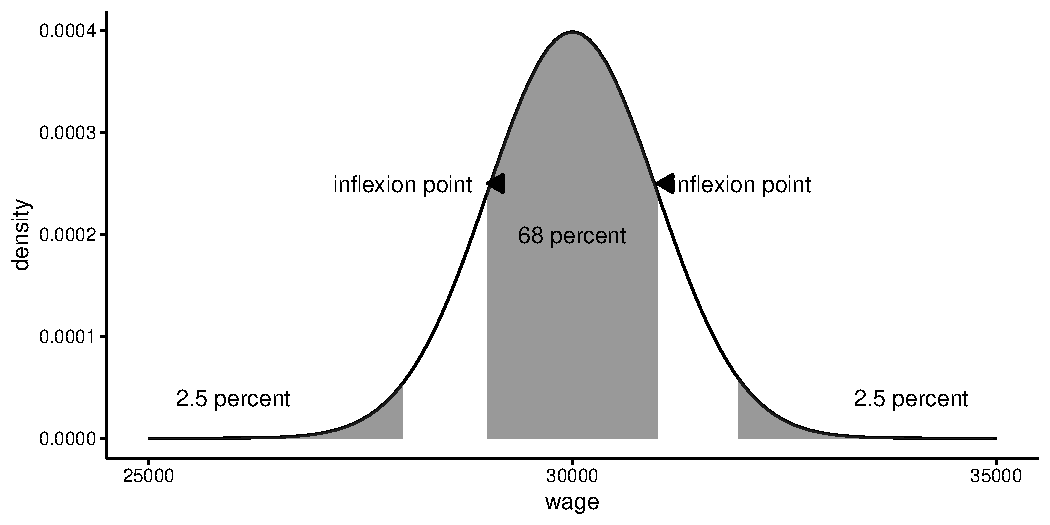
\includegraphics[width=\maxwidth]{figure/distr_4-1} 

}

\caption[The theoretical normal distribution with mean 30,000 and standard deviation 1000]{The theoretical normal distribution with mean 30,000 and standard deviation 1000.}\label{fig:distr_4}
\end{figure}


\end{knitrout}

The densities in Figures \ref{fig:densitywages} and \ref{fig:distr_4} look so similar, they are practically indistinguishable.

Mathematicians have discovered many interesting things about the normal distribution. If the distribution of a variable closely resembles the normal distribution, you can infer many things. One thing we know about the normal distribution is that the mean, mode and median are always the same. Another thing we know from theory is that the inflexion points\footnote{The inflexion point is where concave turns into convex, and vice versa. Mathematically, the inflexion point can be found by equating the second derivative of a function to 0.} are one standard deviation away from the mean.  Figure \ref{fig:distr_4} shows the two inflexion points. From theory we also know that if a variable has a normal distribution, 68\% of the observed values lies between these two inflexion points. We also know that 5\% of the observed values lie more than 1.96 standard deviations away from the mean (2.5\% on both sides, see Figure \ref{fig:distr_4}). Theorists have constructed tables that make it easy to see what proportion of values lies more than $1, 1.1, 1.2 \dots, 3.8, 3.9, \dots$ standard deviations away from the mean. These tables are easy to find online or in books, and these are fully integrated into statistical software like SPSS and R. Because all these percentages are known for the number of standard deviations, it is easier to talk about the \textit{standard normal distribution}.

In such tables, you find information only about the \textit{standard normal distribution}. The standard normal distribution is a normal distribution where all values have been \textit{standardized} (see Section \ref{sec:standarddeviation}). Standardized means that the values have an average of 0 and a standard deviation of 1. Such standardized values are obtained if you subtract the mean score from each value, and divide the result by the standard deviation. A standardized value is often denoted as a $Z$-score. Thus in formula form, a value $x$ is standardized by using the following equation:


\begin{equation}
Z = \frac{x - \bar{x}}{\sigma}
\end{equation}



% latex table generated in R 3.5.0 by xtable 1.8-2 package
% Mon Jan 21 16:42:09 2019
\begin{table}[ht]
\centering
\caption{Standardizing scores.} 
\label{tab:normal_1}
\begin{tabular}{rrrr}
  \hline
x & mean & x\_minus\_mean & Z \\ 
  \hline
7.2 & 10.4 & -3.2 & -0.7 \\ 
  8.8 & 10.4 & -1.5 & -0.3 \\ 
  17.8 & 10.4 & 7.4 & 1.6 \\ 
  10.4 & 10.4 & -0.0 & -0.0 \\ 
  10.6 & 10.4 & 0.3 & 0.1 \\ 
  18.6 & 10.4 & 8.2 & 1.7 \\ 
  12.3 & 10.4 & 1.9 & 0.4 \\ 
  3.7 & 10.4 & -6.7 & -1.4 \\ 
  6.6 & 10.4 & -3.8 & -0.8 \\ 
  7.8 & 10.4 & -2.6 & -0.5 \\ 
   \hline
\end{tabular}
\end{table}


Table \ref{tab:normal_1} shows an example set of $x$-values that are standardized. The average of the $x$-values turns out to be 10.38, and the standard deviation 4.77. By subtracting the mean, we ensure that the average $Z$-score becomes 0, and by subsequently dividing by the standard deviation, we make sure that the standard deviation of the $Z$-scores becomes 1.

This standardization makes it much easier to look up certain facts about the normal distribution. For instance, if we go back to the normally distributed temperature values, we see that the average is 30000, and the standard deviation is 1000. Thus, if we take all wages, subtract 30000 and divide by 1000, we get standardized wages with average 0 and standard deviation 1. The result is shown in Figure \ref{fig:normal_2}. We know that the inflexion points lie at one standard deviation below and above the mean. The mean is 30000, and the standard deviation equals 1000, so the inflexion points are at $30000-1000=29000$ and $30000+1000=31000$. Thus we know that 68\% of the wages are between 29000 and 31000.


\begin{knitrout}
\definecolor{shadecolor}{rgb}{0.969, 0.969, 0.969}\color{fgcolor}\begin{figure}

{\centering 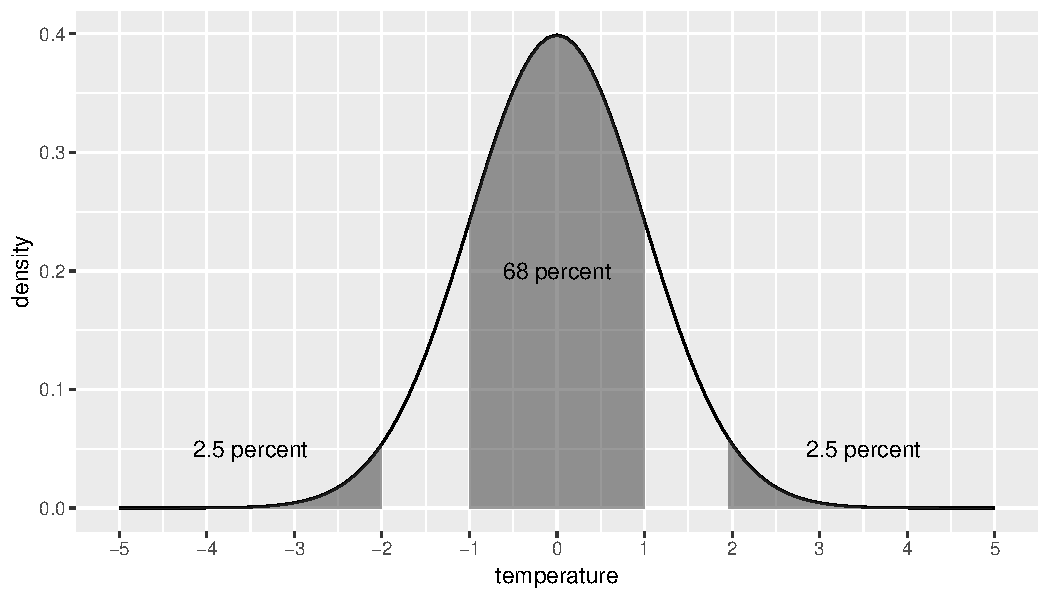
\includegraphics[width=\maxwidth]{figure/normal_2-1} 

}

\caption[The standard normal distribution]{The standard normal distribution.}\label{fig:normal_2}
\end{figure}


\end{knitrout}

How do we know that 68\% of the observations lie between the two inflexion points? Similar to proportions and cumulative proportions, we can plot the cumulative normal distribution. Figure \ref{fig:normal_3} shows the cumulative proportions curve for the normal distribution. Note that we no longer see dots because the variable z is continuous.

\begin{knitrout}
\definecolor{shadecolor}{rgb}{0.969, 0.969, 0.969}\color{fgcolor}\begin{figure}

{\centering 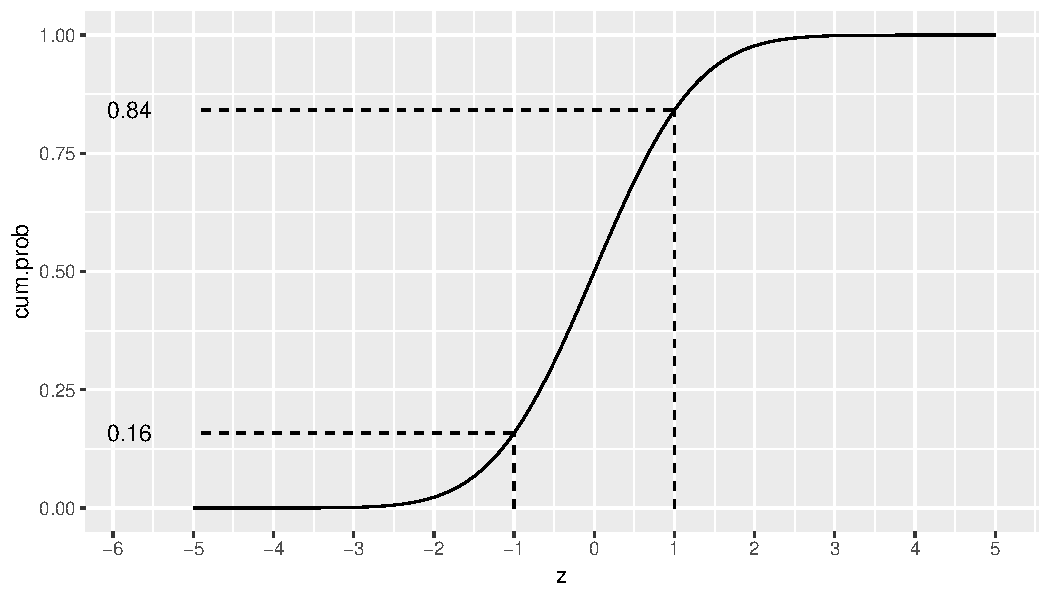
\includegraphics[width=\maxwidth]{figure/normal_3-1} 

}

\caption[The cumulative standard normal distribution]{The cumulative standard normal distribution.}\label{fig:normal_3}
\end{figure}


\end{knitrout}

We know that the two inflexion points lie one standard deviation below and above the mean. Thus, if we look at a $z$-values of 1, we see that the cumulative probability equals about 0.8413447. This means that 84.1344746 \% of the $z$-values are lower than 1. If we look at a $z$-values of -1, we see that the cumulative probability equals about 0.1586553. This means that 15.8655254 \% of the $z$-values are lower than -1. Therefore, if we want to know what percentage of the $z$-values lie between -1 and 1, we can calculate this by subtracting 0.1586553 from 0.8413447, which equals 0.6826895, which corresponds to slightly over 68\%.

All quantiles for the standard normal distribution can be looked up online\footnote{see for example ....} or in books. Table \ref{tab:normal_4} gives a short list of quantiles. From this table, you see that 1\% of the $z$-values is lower than -2.33, and that 25\% of the $z$-values is lower than -0.67. We also see that half of all the $z$-values is lower than 0.00 and that 10\% of the $z$-values is larger than 1.28, and that the 1\% largest values are higher than 2.33.

% latex table generated in R 3.5.0 by xtable 1.8-2 package
% Mon Jan 21 16:42:09 2019
\begin{table}[ht]
\centering
\caption{Some quantiles for the standard normal distribution.} 
\label{tab:normal_4}
\begin{tabular}{rr}
  \hline
cum.proportion & z \\ 
  \hline
0.01 & -2.33 \\ 
  0.10 & -1.28 \\ 
  0.25 & -0.67 \\ 
  0.50 & 0.00 \\ 
  0.75 & 0.67 \\ 
  0.90 & 1.28 \\ 
  0.99 & 2.33 \\ 
   \hline
\end{tabular}
\end{table}



Thus, if we return to our temperatures with mean 30000 and standard deviation 1000, we know from Table \ref{tab:normal_4} that 99\% of the temperatures are below 30000 + 2.33 times the standard deviation =  $30000+2.33*1000$=32330.

Returning back to the IQ example of Section \ref{sec:standarddeviation}. Suppose we have IQ scores that are normally distributed with a mean of 100 and a standard deviation of 15. What IQ score would be the 90th percentile? From Table \ref{tab:normal_4} we see that the 90th percentile is a $Z$-value of 1.28. Thus,the 90th percentile for our IQ scores lies 1.28 standard deviations above the mean (above because the $Z$-value is positive. The mean is 100 so we have to look at 1.28 standard deviations above that. The standard deviation equals 15, so we have to look at an IQ score of $100 + 1.28 \times 15$, which equals 119.2. This tells us that 90\% of the IQ scores are equal to or lower than 119.2.

As a last example, suppose we have a personality test that measures extraversion. If we know that test scores are normally distributed with a mean of 18 and a standard deviation of 2, what would be the 0.10 quantile? From Table \ref{tab:normal_4} we see that the 0.10 quantile is a Z-value of -1.28. This tells us that the 0.10 quantile for the personality scores lies at 1.28 standard deviations below the mean. The mean is 18, so the 0.10 quantile for the personality scores lies at 1.28 standard deviations below 18. The standard deviation is 2, so this amounts to $18-1.28 \times 2= 15.44$. This tells us that 10\% of the scores on this test are 15.44 or lower.

Such handy tables are also available for other theoretical distributions. Theoretical distributions are at the core of many data analysis techniques, including linear models. In this book, apart from the normal distribution, we will also encounter other theoretical distributions: the $t$-distribution (\fref{chap:confidence}), the $F$-distribution (\fref{chap:categorical}), the chi-square distribution (\fref{chap:poisson}) and the Poisson distribution (\fref{chap:poisson}).

% \subsection{The chi-square distribution}
% Suppose that we have 1,000 temperature measures from one location. Say that these measures were taken on 1000 different days, so that for each day, temperature was measured once randomly during the day. If we compute, for every day, the squared deviation of the observed temperature from the average temperature, and we plot these 1000 different values, we might get something like is shown in Figure \ref{fig:distr_5}. This in turn bears close resemblance to another theoretical distributution, the chi-square distibution (or $\chi^2$-distribution). This $\chi^2$-distribution is plotted in Figure \ref{fig:distr_6}. For this distribution, there are also tables that tell us the percentage of observed values that are equal to or smaller than a particular value, say 5. For example, we know from theory that for the chi-square distribution depicted in Figure \ref{fig:distr_5}, that 95\% of the values is smaller than 3.84.
% 
% <<distr_5, fig.height=4, echo=T, fig.align='center', warning=T, fig.cap='Density plots of 1000 observed squared deviations from the average temperature.' >>=
% set.seed(1234)
% data_frame(temperature = rnorm(1000,30000, 1), day=rep(1:1000)) %>%
%         group_by(day) %>%
%         summarise(SS=(temperature-30000)^2) %>%
%         ggplot()+
%         geom_density(aes(x=SS)) +
%         ylab("density") + xlab("Temperature minus average temperature squared")+
%         xlim(c(0,10))
% @
% %
% 
% %%%% something goes wrong when running with this figure below that didnt go wrong before. something to doe with \vref or \vpageref (may loop) package varioref error
% 
% 
% <<distr_6, fig.height=2, echo=T, message=T, fig.align='center', warning=T, fig.cap='The theoretical chi-square distribution' >>=
% shaded <-  data_frame(x = seq(3.84, 10,0.1),  y = dchisq(seq(3.84, 10,0.1), 1, 0))
% data_frame(temperature = seq(0.18,10,0.1)) %>%
%         ggplot()+
%         geom_line(aes(x=temperature, y = dchisq(temperature,df=1, ncp=0))) +
%         geom_area(data=shaded, mapping = aes(x=x ,  y=y),alpha=0.5)+
%         ylab("density") + xlab("chi-square")
%         xlim(c(0,10)) +
%         geom_text(x=3.84,y=-0.01, label=paste(3.84))+
%           geom_text(x=5.5, y=0.05, label="5 percent")
%  @
% %
%


\section{Visualizing numeric variables: the boxplot}

We started this chapter with variables that can be stored in a data matrix. With a variable with a large number of values on a large number of units of analysis, it is hard to get a an intuitive feel for the data. Making a frequency table is one way of summarizing a variable, computing meaurures of central tendency and variation is another way. Visualization is probably the best way of getting a quick and dirty feel for the information contained in a large data matrix. Earlier in this chapter we came across frequency plots, histograms, and density plots to visualize the distribution of a single variable. A fourth plot for a single variable that we discuss in this book is the \textit{boxplot}.  

A boxplot gives a quick overview of the distribution of a numeric variable in terms of its quartiles. Figure \ref{fig:chis_7} gives an example of a boxplot of (part of) the wage data. The white box represents the interquartile range. The top of the white box equals the third quartile, and the bottom of the white box equals the first quartile. Therefore, we know that half of the workers have a wage between 29,400 and 30,800 The horizontal black lines within the white box represents the second quartile (the median), so half of the workers earn less 30,100. 

A boxplot also shows whiskers: two vertical lines sprouting from the white box. There are several ways to draw these two whiskers. One way is to draw the the top whisker to the largest value (the maximum) and the bottom whisker to the smallest value (the minimum). This is the default way that SPSS uses. Another way is to have the upper whisker extend from the third quartile to the value equal to 1.5 times the interquartile range, and the lower whisker (the vertical line on top of the box) extends from the first quartile to the value equal to -1.5 times the interquartile range (the interquartile range is of course the height of the white box). The dots are outlying values, or simply called \textit{outliers}. This is displayed in Figure \ref{fig:chis_7}. There you see first and third quartiles of 29,400 and 30,800, respectively, so an interquartile range (IQR) of $30800-29400=1400$. Multiplying this IQR by 1.5 we get $1.5 \times 1400= 2100$. The whiskers therefore extend to $29400-2100=27300$ and $30800+2100=32900$. 

Thus, the boxplot is a quick way of visualizing in what range the middle half of the values are (the range in the white box), where most of the values are (the range of the white box plus the whiskers), and where the extreme values are (indvidually plotted as dots). Note that the white box always contains 50\% of the values. The whiskers are only extensions of the of the box by a factor of 1.5. In many cases you see that they contain most of the values, but sometimes they miss a lot of values. You will see that when you notice a lot of outliers.

\begin{knitrout}
\definecolor{shadecolor}{rgb}{0.969, 0.969, 0.969}\color{fgcolor}\begin{figure}

{\centering 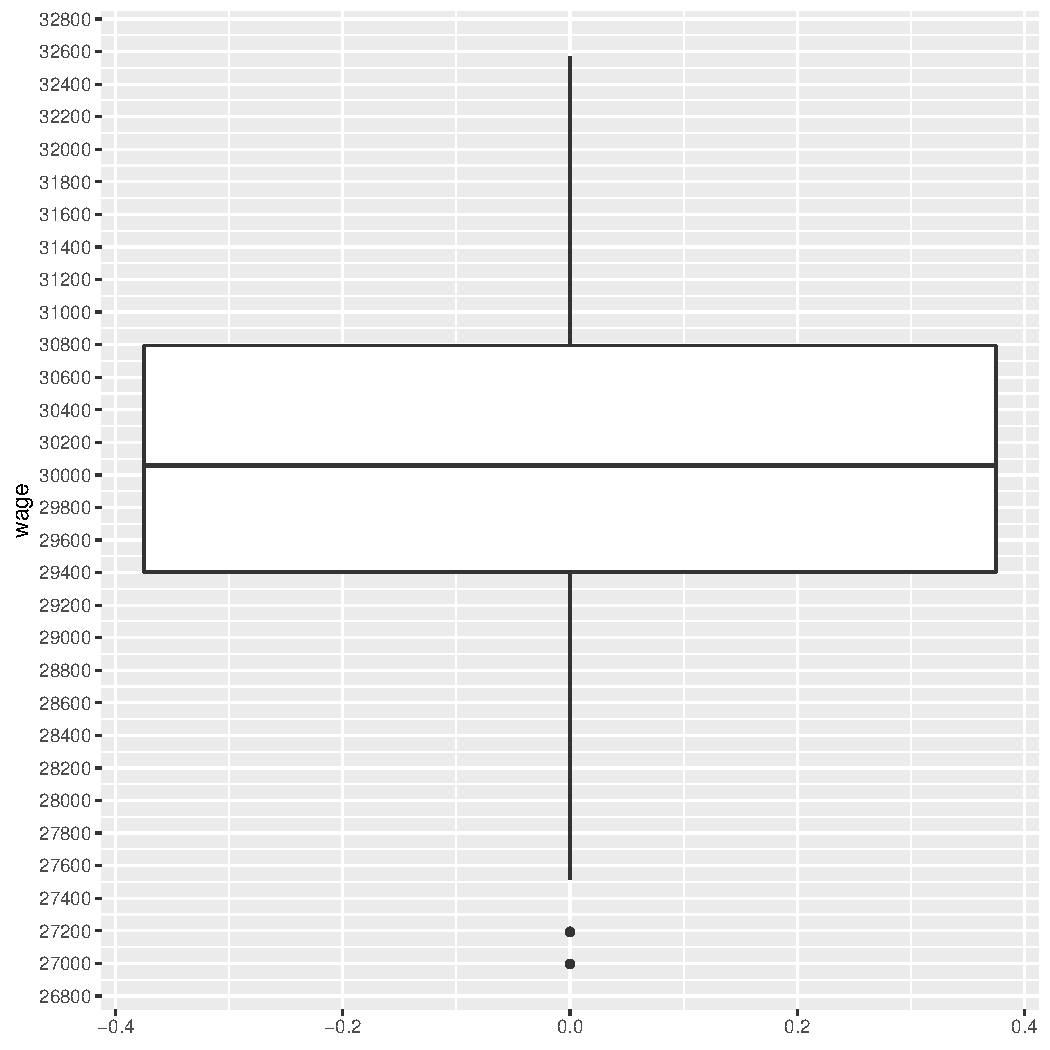
\includegraphics[width=\maxwidth]{figure/chis_7-1} 

}

\caption[A boxplot of the wages earned by a sample of 150 administrative clerks]{A boxplot of the wages earned by a sample of 150 administrative clerks}\label{fig:chis_7}
\end{figure}


\end{knitrout}




\section{Visualizing categorical variables}

The histogram, the density plot and the boxplot can be used for numeric variables, but also for ordinal variables that you'd like to treat numerically. For categorical variables and ordinal variables that can't be treated numerically, we need other types of plots.

For example, suppose we are in a lecture hall with 456 students and we count the number of Dutch, German, Belgian, Indian, Chinese and Indonesian students. We could summarize the results in a frequency table (see Figure \ref{tab:nationality_1}), but a \textit{bar chart} shows the distribution in a much more dramatic way, see Figure \ref{fig:nationality_2}.



% latex table generated in R 3.5.0 by xtable 1.8-2 package
% Mon Jan 21 16:42:09 2019
\begin{table}[ht]
\centering
\caption{A frequency table of nationalities.} 
\label{tab:nationality_1}
\begin{tabular}{rr}
  \hline
 & . \\ 
  \hline
Chinese & 12 \\ 
  Dutch & 141 \\ 
  German & 278 \\ 
  Indian & 12 \\ 
  Indonesian & 13 \\ 
   \hline
\end{tabular}
\end{table}


\begin{knitrout}
\definecolor{shadecolor}{rgb}{0.969, 0.969, 0.969}\color{fgcolor}\begin{figure}

{\centering 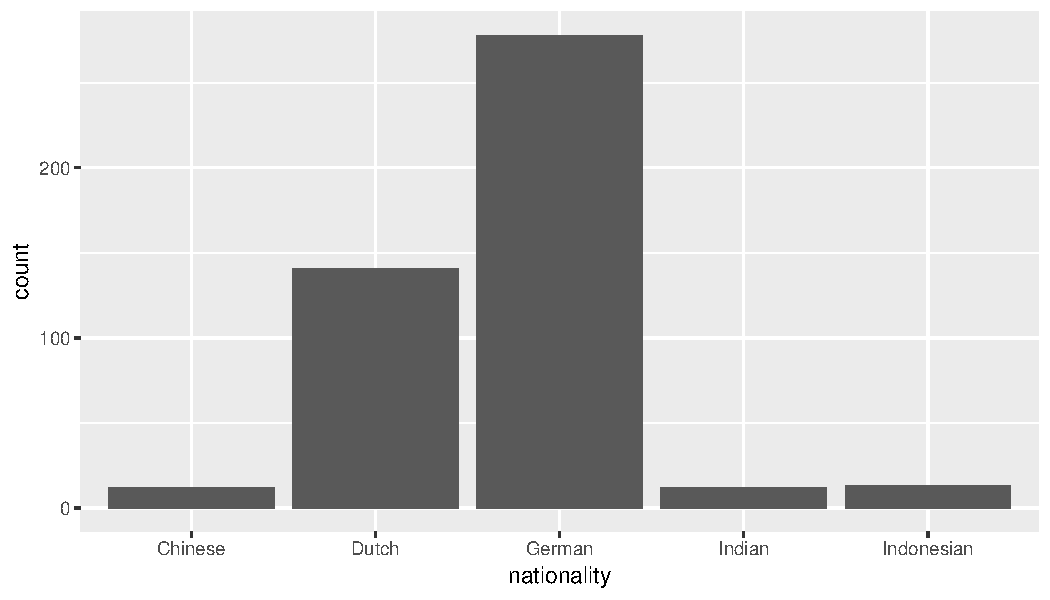
\includegraphics[width=\maxwidth]{figure/nationality_2-1} 

}

\caption[A bar chart of the observed nationalities in a lecture hall]{A bar chart of the observed nationalities in a lecture hall.}\label{fig:nationality_2}
\end{figure}


\end{knitrout}

Sometimes, counts of values of a categorical variable are displayed as a \textit{pie chart}, see Figure \ref{fig:nationality_3}. Pie charts are however best avoided. First, because compared to bar charts, they show no information about the actual counts; you only observe relative sizes of the counts. Second, it is very hard to see from a pie chart what the exact proportions are. For example, from the bar chart in Figure \ref{fig:nationality_2} it is easily seen that the ratio German students to Dutch students is about 2 to 1. Research shows that this ratio cannot be read with the same precision from the pie chart in Figure \ref{fig:nationality_3}. In sum, pie charts are best replaced by bar charts.



\begin{knitrout}
\definecolor{shadecolor}{rgb}{0.969, 0.969, 0.969}\color{fgcolor}\begin{figure}

{\centering 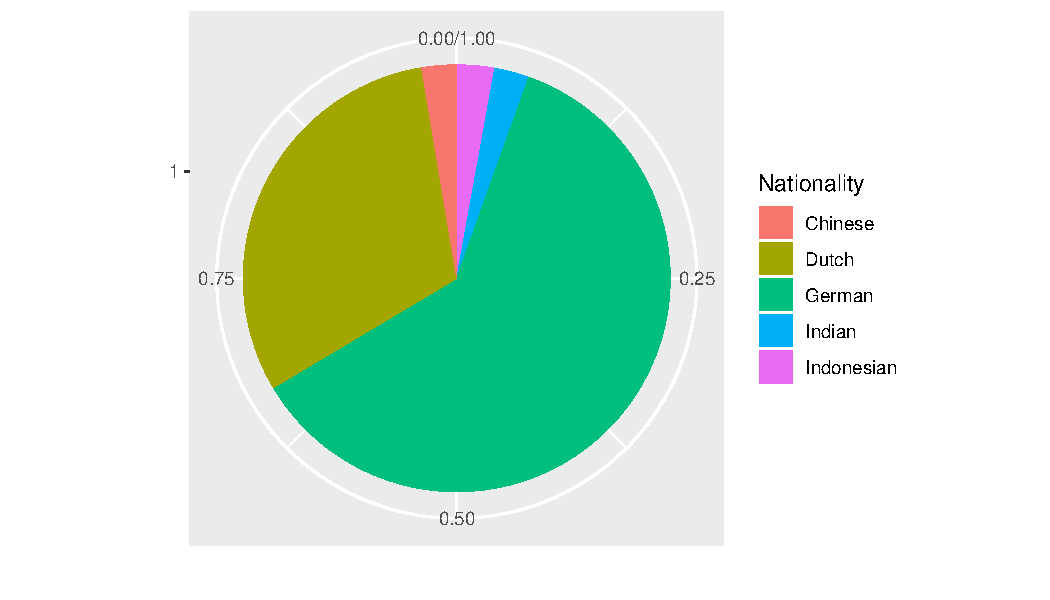
\includegraphics[width=\maxwidth]{figure/nationality_3-1} 

}

\caption[A bar chart of nationalities]{A bar chart of nationalities.}\label{fig:nationality_3}
\end{figure}


\end{knitrout}


Ordinal variables are usually best visualized using bar charts. Figure \ref{fig:climate_1} shows the variation of the answers to a Likert questionnaire item, where Nairobi inhabitants are asked "To what degree do you agree with the statement that the climate in Iceland is agreeable?". With ordinal variables, make sure that the labels are are in the natural order. 

\begin{figure}

{\centering 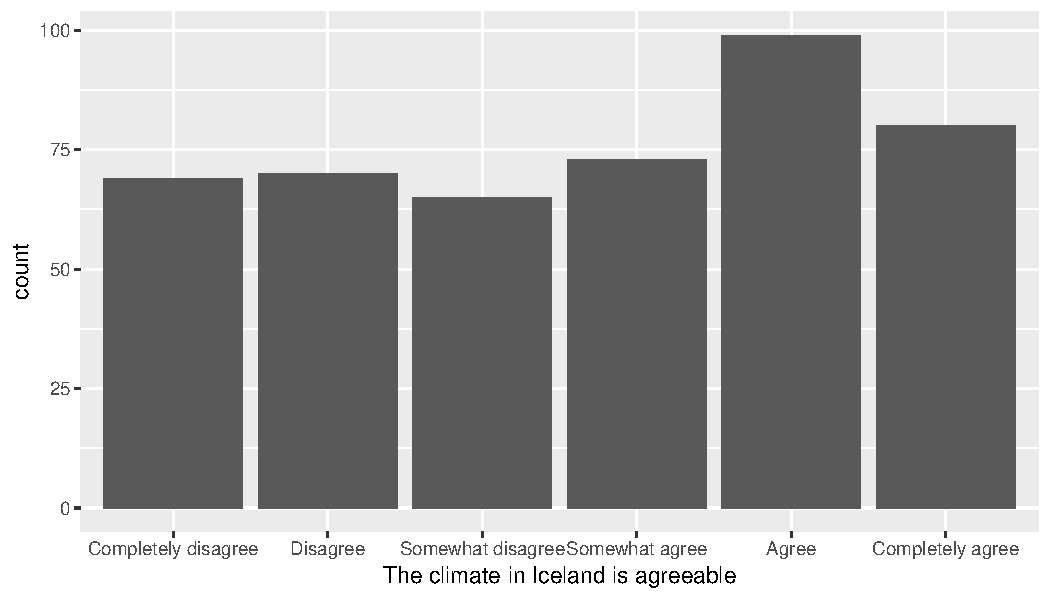
\includegraphics[width=\maxwidth]{figure/climate_1-1} 

}

\caption[Opinions on the climate in Iceland]{Opinions on the climate in Iceland.}\label{fig:climate_1}
\end{figure}





\section{Visualizing co-varying variables}

\subsection{Categorical by categorical: crosstable}

Variables are properties that vary: from person to person, or from location to location, or from time to time, of from object to object. Sometimes when you have two variables, you see that they co-vary: when one variable changes, the other variable changes too. For example, suppose I have 20 pencils. These pencils may vary in colour: twelve of them are red, and eight of them are blue. Therefore, colour is a variable with values "red" and "blue". The twenty pencils also vary in length: four are unused and therefore still long, and sixteen of them have been used many times so that they are short. Therefore, length is also a variable, with values "long" and "short". Note that these variables have been measured using the same pencils. In theory I could have long blue pencils, long red pencils, short blue pencils and short red pencils. Let's look at the pencils that I have: for each combination of lenght and colour, I count the number of pencils. The result I put in Table \ref{tab:crosstable_1}.

% latex table generated in R 3.5.0 by xtable 1.8-2 package
% Mon Jan 21 16:42:11 2019
\begin{table}[ht]
\centering
\caption{Crosstabulation of colour and length for twenty pencils.} 
\label{tab:crosstable_1}
\begin{tabular}{rrr}
  \hline
 & blue & red \\ 
  \hline
long & 0 & 4 \\ 
  short & 8 & 8 \\ 
   \hline
\end{tabular}
\end{table}


Such a table is called a \textit{crosstable}. For every combination of two variables, I see the number of objects (units of analysis) that have that combination. From the table we see that there is not a single pencil that is both red and long (count is 0). At the same time you also see that all long pencils are blue. A crosstable is therefore a nice way to show how two variables co-vary. From this particular table for instance, you can easily see that once you know that a pencil is long, you automatically know it is blue.


Crosstables are nice visualization of how two categorical variables co-vary. But what if one of the two variables is not a categorical variable?


\subsection{Categorical by numerical: boxplot}
Suppose instead of determining length by values "short" and "long", I could measure the exact length of the pencils in centimeters. I put the results in Table \ref{tab:crosstable_2}. We see that the table is much larger than Table \ref{tab:crosstable_1}. We also see quite a few cells with zeros. In most cases, for every particular combination of length and colour we only see a count of 1 pencil. In general, you see that when one of the variables is numeric, the crosstable becomes very large and in addition it becomes sparse, that is, with many zeros. With such a large and sparse table, it is hard to get a quick impression of how two variables co-vary.

% latex table generated in R 3.5.0 by xtable 1.8-2 package
% Mon Jan 21 16:42:11 2019
\begin{table}[ht]
\centering
\caption{Crosstabulation of colour and length for twenty pencils.} 
\label{tab:crosstable_2}
\begin{tabular}{rrr}
  \hline
 & blue & red \\ 
  \hline
2 &   1 &   0 \\ 
  2.7 &   0 &   1 \\ 
  3.3 &   0 &   1 \\ 
  3.4 &   1 &   0 \\ 
  3.5 &   1 &   0 \\ 
  3.6 &   0 &   1 \\ 
  4.1 &   1 &   1 \\ 
  4.4 &   1 &   1 \\ 
  4.5 &   1 &   1 \\ 
  4.7 &   1 &   0 \\ 
  5.2 &   0 &   1 \\ 
  5.7 &   0 &   1 \\ 
  5.8 &   1 &   0 \\ 
  9 &   0 &   4 \\ 
   \hline
\end{tabular}
\end{table}



The alternative for two variables where one is categorical and the other one is numeric, is to create a \textit{boxplot}. Figure \ref{fig:crosstable_3} shows a boxplot of the pencil data. A boxplot gives a quick overview of the distribution of the pencils: one distribution of the blue pencils, and one distribution of the red pencils. Let's first have a look at the blue pencils on the left side of the plot. The white box represents the interquartile range, so that we know that half of the blue pencils have a height between 3.5 and 4.5. The horizontal black lines within the white box represents the median, so half of the blue pencils is shorter than 4.3. The upper whisker (the vertical line on top of the box) extends from the third quartile to the value equal to 1.5 times the interquartile range, and the lower whisker (the vertical line on top of the box) extends from the first quartile to the value equal to -1.5 times the interquartile range.

\begin{figure}

{\centering 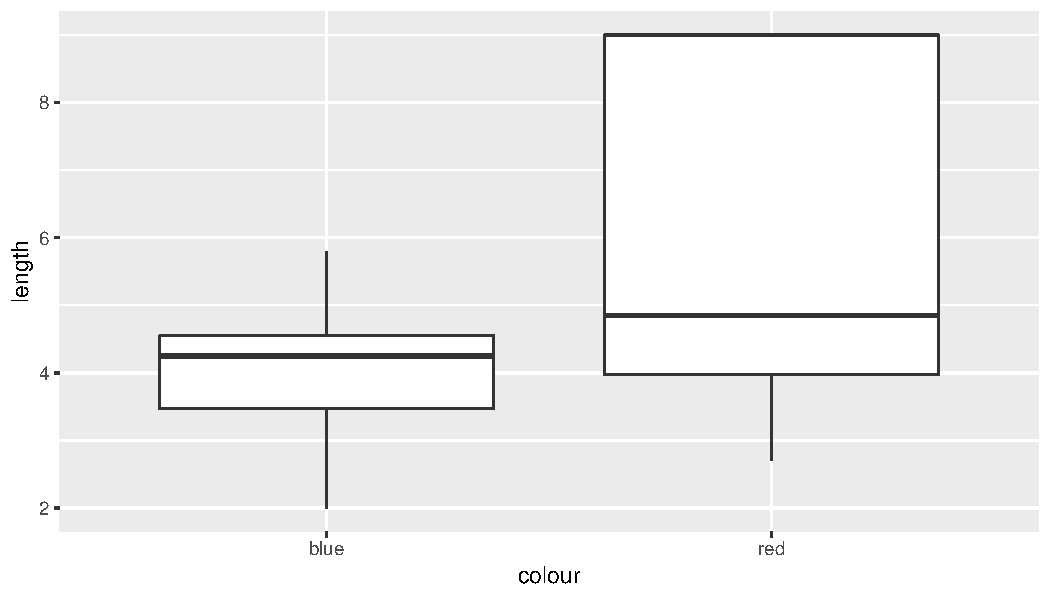
\includegraphics[width=\maxwidth]{figure/crosstable_3-1} 

}

\caption[A boxplot of the pencil data]{A boxplot of the pencil data.}\label{fig:crosstable_3}
\end{figure}



From a boxplot like this it is easy to spot differences in the distribution of a quantitative measure for different levels of a qualitative measure. From Figure \ref{fig:crosstable_3} we easily spot that the blue pencils (varying between 2 and 6 cm) tend to be shorter than the red pencils (varying between 4 and 9 cm). Thus, in these pencils, length and colour tend to co-vary: blue pencils are often short and red pencils are often long.


\subsection{Numeric by numeric: scatterplot}

% latex table generated in R 3.5.0 by xtable 1.8-2 package
% Mon Jan 21 16:42:11 2019
\begin{table}[ht]
\centering
\caption{Crosstabulation of length (rows) and weight (columns) for twenty pencils.} 
\label{tab:crosstable_4}
\begin{tabular}{rrrrrrr}
  \hline
 & 3.3 & 3.4 & 3.5 & 3.6 & 3.7 & 4 \\ 
  \hline
2 &   1 &   0 &   0 &   0 &   0 &   0 \\ 
  2.7 &   0 &   1 &   0 &   0 &   0 &   0 \\ 
  3.3 &   0 &   1 &   0 &   0 &   0 &   0 \\ 
  3.4 &   0 &   1 &   0 &   0 &   0 &   0 \\ 
  3.5 &   0 &   0 &   1 &   0 &   0 &   0 \\ 
  3.6 &   0 &   0 &   1 &   0 &   0 &   0 \\ 
  4.1 &   0 &   0 &   2 &   0 &   0 &   0 \\ 
  4.4 &   0 &   0 &   2 &   0 &   0 &   0 \\ 
  4.5 &   0 &   0 &   2 &   0 &   0 &   0 \\ 
  4.7 &   0 &   0 &   0 &   1 &   0 &   0 \\ 
  5.2 &   0 &   0 &   0 &   1 &   0 &   0 \\ 
  5.7 &   0 &   0 &   0 &   0 &   1 &   0 \\ 
  5.8 &   0 &   0 &   0 &   0 &   1 &   0 \\ 
  9 &   0 &   0 &   0 &   0 &   0 &   4 \\ 
   \hline
\end{tabular}
\end{table}



\begin{figure}

{\centering 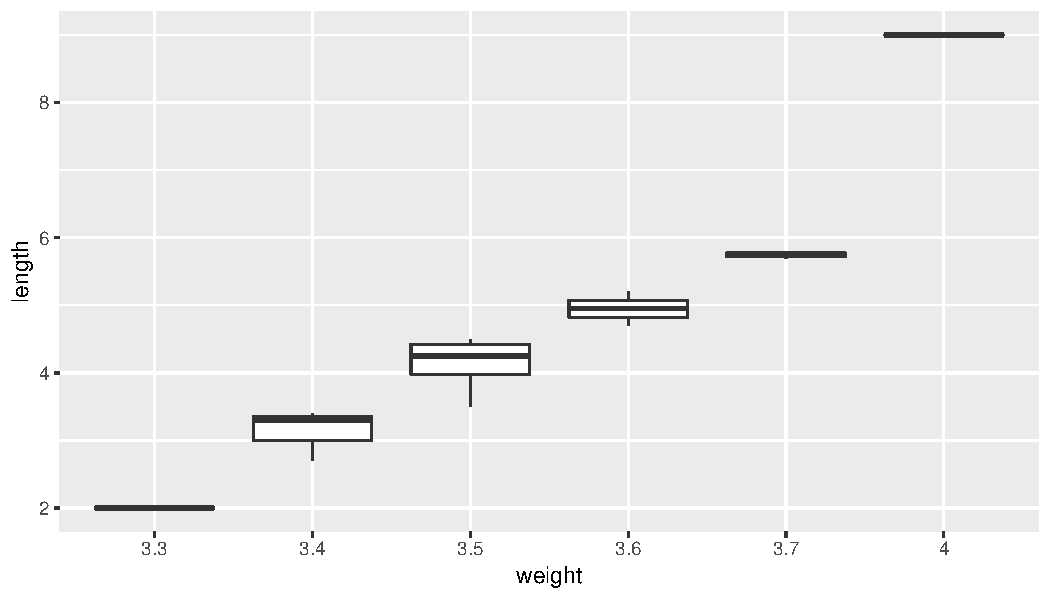
\includegraphics[width=\maxwidth]{figure/crosstable_5-1} 

}

\caption[A boxplot of the pencil data]{A boxplot of the pencil data.}\label{fig:crosstable_5}
\end{figure}



Suppose I also measure the weight of my pencils in grams. Table \ref{tab:crosstable_4} shows the crosstabulation of length and weight. This is a very sparse table (i.e., with lots of zeros), which makes it very hard to see any systematic co-variation in weight and length. Figure \ref{fig:crosstable_5} shows a boxplot of weight and length. Also this plot seems a bit strange, because for every observed weight value under 4 grams, there is only one observation, so that only the median can be plotted.


Therefore, in cases where we have two numeric variables, we generally use a \textit{scatterplot}. Figure \ref{fig:scatter_1} shows a scatterplot of weight by length. Now, the relationship between height and length is easily understood: it appears there is a \textit{linear} relationship between weight. For every increase in weight, there is also an increase in length. The relationship is called linear because we could summarize the relationship by drawing a straight line. This line is shown in Figure \ref{fig:line_1}.


\begin{figure}

{\centering 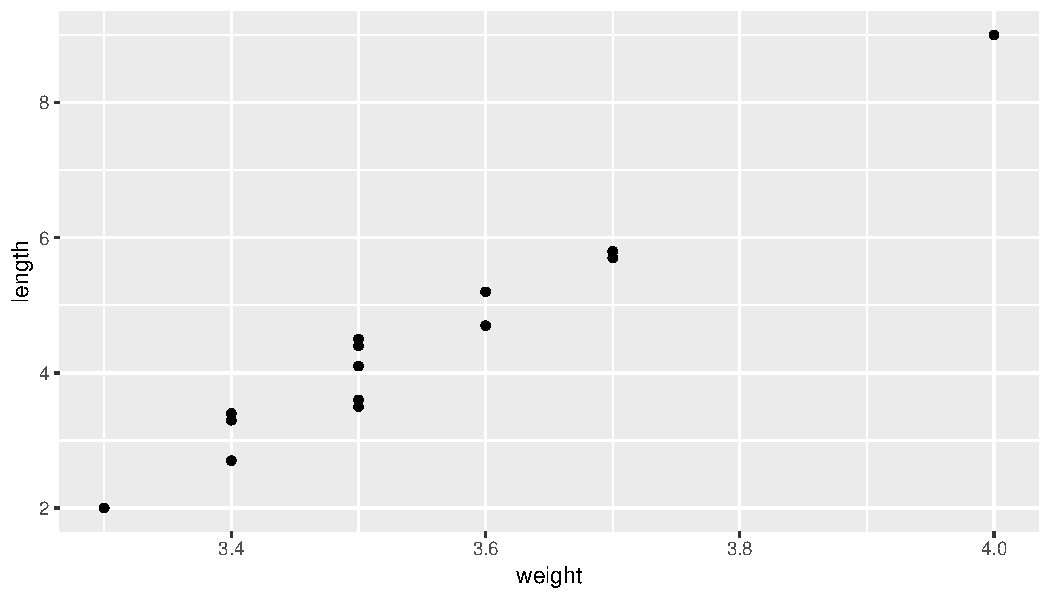
\includegraphics[width=\maxwidth]{figure/scatter_1-1} 

}

\caption[A scatterplot of length and weight]{A scatterplot of length and weight.}\label{fig:scatter_1}
\end{figure}



\begin{figure}

{\centering 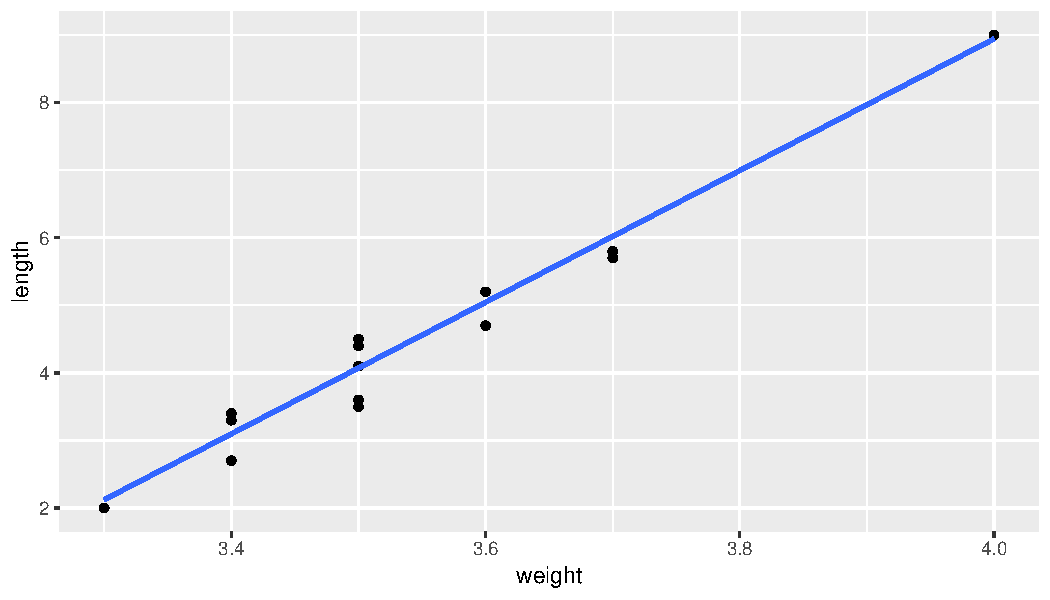
\includegraphics[width=\maxwidth]{figure/line_1-1} 

}

\caption[A scatterplot of length and weight, with a straight line that summarizes the relationship]{A scatterplot of length and weight, with a straight line that summarizes the relationship.}\label{fig:line_1}
\end{figure}



You see that by visualizing two variables, important patterns may emerge that you can easily overlook when only looking at the values. Crosstables, boxplots and scatterplots are powerful tools to find regularities but also oddities in your data that you'd otherwise miss. Some such patterns can be summarized by straight lines, as we see in Figure \ref{fig:line_1}. The remainder of this book focuses on how we can use straight lines to summarize data, but also how to make predictions for data that we have not seen yet.


\section{Overview of the book}

Chapter \ref{chap:simple} will look at how we can use a straight line to summarize the relationship between two numeric variables. A straight line that summarizes your data is a simple case of an \textit{linear model}. In Chapters \ref{chap:confidence} and \ref{chap:hypothesis} we will discuss how you can draw conclusions about data that you have not seen. For example, in the previous section we described the relationship between weight and height of twenty pencils. The question that you may have is whether this linear relationship also holds for \textit{all} pencils of the same make, that is, whether the same linear model holds for both the observed twenty pencils and the total collection of pencils.

In Chapter \ref{chap:multip} we describe how we can use straight lines (linear models) to summarize relationships between more than two numeric variables, and in Chapter \ref{chap:categorical} we will show how we can use straight lines to summarize relationships with independent variables that we want to treat as categorical. Chapter \ref{chap:advanced} shows how you can make elaborate statements about differences between groups of observations, in the case one of the variables is a categorical variable.

Chapter \ref{chap:moderation} focuses on moderation: how one variable can affect the effect that a second variable has on the outcome on a third variable.

Chapter \ref{chap:assumptions} discusses when it is appropriate to use linear models to summarize your data, and when it is not. It shows methods that enable you to decide whether to trust a linear model or not. Chapter \ref{chap:nonpar1} then discussses alternative methods that you can use when linear models are not appropriate.

Chapters \ref{chap:mixed} and \ref{chap:premidpost} show how to deal with variables that are measured more than once in the same research unit (the same participant, the same pencil, the same school, etc.). For example, you may measure the weight of a pencil before and after you have made a drawing with it. Models that we use for such data are called \textit{linear mixed models}. Similar to linear models, linear mixed models are not always appropriate. Therefore, Chapter \ref{chap:nonpar2} discusses alternative methods to study variables that are repeatedly measured in the same research unit.

The book ends with Chapters \ref{chap:logistic} and \ref{chap:poisson} that discuss \textit{generalized linear models}. These are models where the dependent variable is not numeric and continuous. Chapter \ref{chap:logistic} discusses a method that is appropriate when the dependent variable has only two values, say "yes" and "no", or "pass" and "fail". Chapter \ref{chap:poisson} discusses a method that can be used when the dependent variable is a count variable and therefore discrete, for example the number of children in a classroom, or the number of harvested zucchini from one plant.











 % exploring your data, descriptive statistics


\chapter{Linear modelling: introduction}\label{chap:simple}



\section{Dependent and independent variables}
In the previous chapter we discussed the distinction between numeric, ordinal and categorical variables. In linear modelling, there is also another distinction between variables: \textit{dependent} and \textit{independent} variables. Dependency of a variable is not really a property of a variable but it is the result of a choice of the data analyst. Let's first think about relationships between two variables. Determining whether a variable is to be treated as independent or not, is often either a case of logic or a case of theory. When studying the relationship between the height of a mother and that of her child, the more logical it would be to see the height of the child \textit{as a function} of the height of the mother. This because we assume that the genes are transferred from the mother to the child. The mother comes first, and the height of the child is partly the \textit{result} of the mother's genes that were transmitted during fertilisation. That which is the result is usually taken as the \textit{dependent} variable. The theoretical cause or antecedent is usually taken as the \textit{independent} variable. 

The dependent variable is often called the \textit{response variable}. An independent variable is often called a \textit{predictor variable} or simply \textit{predictor}. Independent variables are also often called explanatory variables.

The dependent variable is usually the most important variable. It is the variable that we'd like to understand better, or perhaps predict better. The independent variable is usually an explanatory variable: it explains why some people have high values for the dependent variable and other people have low values. For instance, we'd like to know why some people are healthier than others. Health may then be our dependent variable. An explanatory variable might be age (older people tend to be less healthy), or perhaps occupation (being a dive instructor induces more health problems than being a university teacher). 

Sometimes we're interested to see whether we can predict longevity: age at death is then our dependent variable and our independent (predictor) variables might then be food pattern and genetic make-up. 

Thus, we often see four types of relations:
\begin{itemize}
\item Variable A affects/influences another variable B.
\item Variable A causes variable B.
\item Variable A explains variable B.
\item Variable A predicts variable B.
\end{itemize}

In all these four cases, Variable A is the independent variable and Variable B is the dependent variable.

Note that in general, dependent variables can be either numeric, ordinal, or categorical. Also independent variables can be numeric, ordinal, or categorical. 

\subsection{Exercises}

Below, variables are printed in \textbf{bold}. For each research statement, identify which variable is the dependent variable, and which variable is the independent variable.

\begin{enumerate}

\item The effect of \textbf{income} on \textbf{health}
\item \textbf{Stock value} is affected by \textbf{inflation}
\item \textbf{Size} is influenced by \textbf{weight}
\item \textbf{Shoe size} is predicted by \textbf{sex}
\item The less you \textbf{drink} the more \textbf{thirsty} you become 
\item The more \textbf{calories} you eat, the more you \textbf{weigh}
\item \textbf{Weight} is affected by \textbf{food intake} 
\item \textbf{Weight} is affected by \textbf{exercise} 
\item \textbf{Food intake} is predicted by \textbf{time of year}
\item There is an effect of \textbf{exercise} on \textbf{heart rate} 
\item \textbf{Inflation} leads to higher \textbf{wages} 
\item \textbf{Unprotected sex} leads to \textbf{pregnancy}
\item \textbf{HIV-infection} is caused by \textbf{unprotected sex}
\item The effect of \textbf{alcohol intake} on \textbf{driving performance}
\item \textbf{Sunshine} causes \textbf{growth}


\end{enumerate}

Answers:

\begin{enumerate}

\item \textbf{income} independent, \textbf{health} dependent.
\item \textbf{Stock value} dependent, \textbf{inflation} independent
\item \textbf{Size} dependent, \textbf{weight} independent
\item \textbf{Shoe size} dependent, \textbf{sex} independent
\item \textbf{drink} independent, \textbf{thirsty} dependent
\item \textbf{calories} independent, \textbf{weigh} dependent
\item \textbf{Weight} dependent, \textbf{food intake} independent
\item \textbf{Weight} dependent, \textbf{exercise} independent
\item \textbf{Food intake} dependent, \textbf{time of year} independent
\item \textbf{exercise} independent, \textbf{heart rate} dependent
\item \textbf{Inflation} independent, \textbf{wages} dependent
\item \textbf{Unprotected sex} independent, \textbf{pregnancy} dependent
\item \textbf{HIV-infection} dependent, \textbf{unprotected sex} independent
\item \textbf{alcohol intake} independent, \textbf{driving performance} dependent
\item \textbf{Sunshine} independent, \textbf{growth} dependent


\end{enumerate}



\section{Linear equations}


\begin{knitrout}
\definecolor{shadecolor}{rgb}{0.969, 0.969, 0.969}\color{fgcolor}\begin{figure}

{\centering 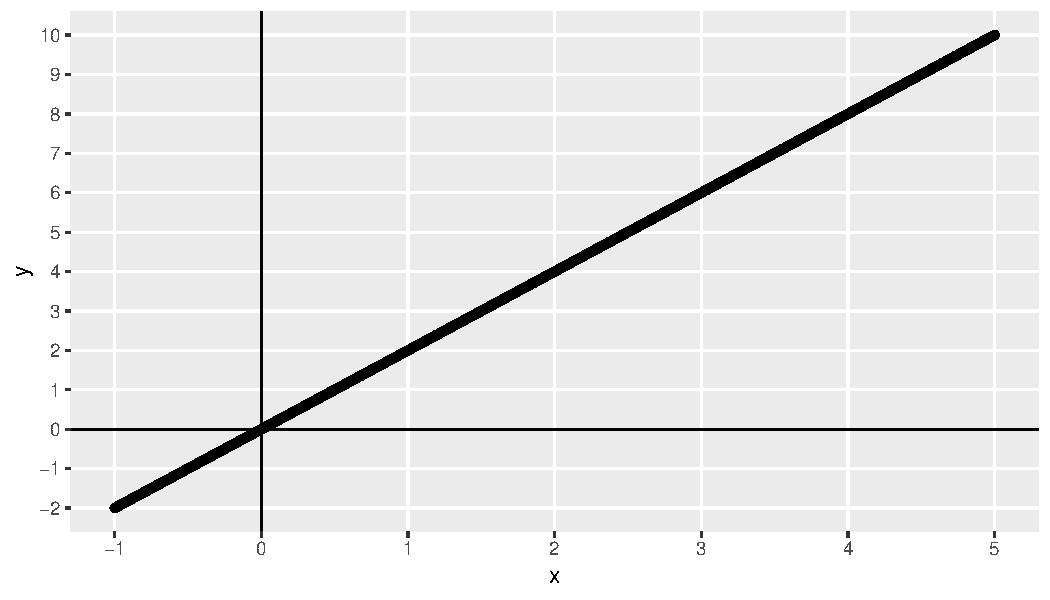
\includegraphics[width=\maxwidth]{figure/lm_1-1} 

}

\caption[Straight line with intercept 0 and slope 2]{Straight line with intercept 0 and slope 2.}\label{fig:lm_1}
\end{figure}


\end{knitrout}


From secondary education you might remember linear equations. Suppose you have two quantities, $x$ and $y$, and there is a straight line that describes best their relationship. An example is given in Figure \ref{fig:lm_1}. We see that for every value of $x$, there is only one value of $y$. Moreover, the larger the value of $x$, the larger the value of $y$. If we look more closely, we see that for each increase of 1 unit in $x$, there is an increase of 2 units in $y$. For instance, if $x=1$, we see a $y$ value of 2, and if $x=2$ we see a $y$-value of 4. So if we move from $x=1$ to $x=2$ (a step of one on the $x$-axis), we move from 2 to 4 on the $y$-axis, which is an increase of 2 units. This increase of 2 units for every step of 1 unit in $x$ is the same for all values of $x$ and $y$. For instance, if we move from 9 to 10 on the $x$-axis, we go from 18 to 20 on the $y$-axis: an increase of again 2 units. This constant increase is typical of linear relationships. The increase in $y$ for every unit increase in $x$ is called the \textit{slope} of a straight line. In this figure, the slope is equal to 2.

The slope is one important characteristic of a straight line. The second important property of a straight line is the \textit{intercept}. The intercept is the value of $y$, if $x=0$. In Figure \ref{fig:lm_1} we see that if $x=0$, $y$ is 0, too. Therefore the intercept of this straight line is 0.

With the intercept and the slope, we completely describe this straight line: no other information is necessary. Such a straight line describes a linear relationship between $x$ and $y$. The linear relationship can be formalized using a linear equation. The general form of a linear equation for two variables $x$ and $y$ is the following:

\begin{equation}
y = intercept + slope \times x
\end{equation}


For the linear relationship between $x$ and $y$ in Figure \ref{fig:lm_1} the linear equation is therefore

\begin{equation}
y = 0 + 2 x
\end{equation}

which can be simplified to

\begin{equation}
y =  2 x
\end{equation}


With this equation, we can find the $y$-value for all values of $x$. For instance, if we want to know the $y$-value for $x=3.14$, then using the linear equation we know that $y = 2 \times 3.14 = 6.28$. If we want to know the $y$ value for $x=49876.6$, we use the equation to obtain $y=2\times 49876.6 = 99753.2$. In short, the linear equation is very helpful to quickly say what $y$-value is on the basis of the $x$-value, even if we don't have a graph of the relationship or if the graph does not extent to certain $x$-values.


In the linear equation, we call $y$ the \textit{dependent} variable, and $x$ the \textit{independent} variable. This because the equation helps us determine our value of $y$ on the basis of what we know about the value of $x$. When we graph the line that the equation represents, such as in Figure \ref{fig:lm_1}, the common way is to put the dependent variable on the vertical axis, and the independent variable on the horizontal axis. 


Figure \ref{fig:lm_2} shows a different linear relationship between $x$ and $y$. First we look at the slope: we see that for every unit increase in $x$ (from 1 to 2, or from 4 to 5) we see an increase of 0.5 in $y$. Therefore the slope is equal to 0.5. Second, we look at the intercept: we see that if $x=0$, $y$ has the value -2. So the intercept is -2. Again, we can describe the linear relationship by a linear equation, which is now:

\begin{equation}
y = -2 + 0.5 x
\end{equation}



\begin{knitrout}
\definecolor{shadecolor}{rgb}{0.969, 0.969, 0.969}\color{fgcolor}\begin{figure}

{\centering 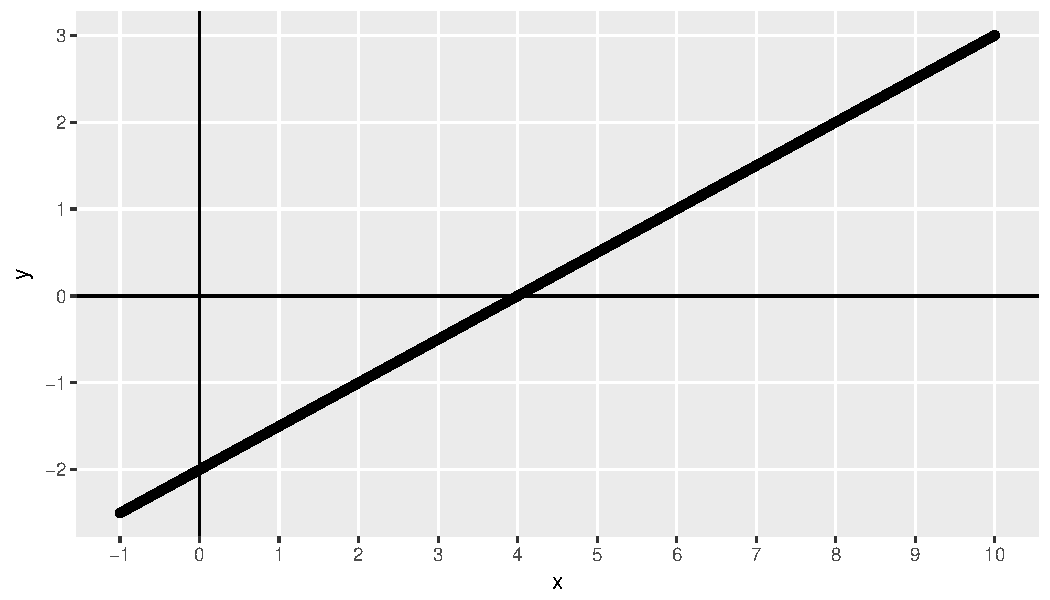
\includegraphics[width=\maxwidth]{figure/lm_2-1} 

}

\caption[Straight line with intercept -2 and slope 0.5]{Straight line with intercept -2 and slope 0.5.}\label{fig:lm_2}
\end{figure}


\end{knitrout}


Linear relationships can also be negative, see Figure \ref{fig:lm_3}. There, we see that if we move from 0 to 1, we see a \textit{decrease} of 2 in $y$ (we move from y=-2 to y=-4), so that is our slope value. Further, if $x=0$, we see a y-value of -2, and that is our intercept. The linear equation is therefore:

\begin{equation}
y = -2 - 2 x
\end{equation}


\begin{knitrout}
\definecolor{shadecolor}{rgb}{0.969, 0.969, 0.969}\color{fgcolor}\begin{figure}

{\centering 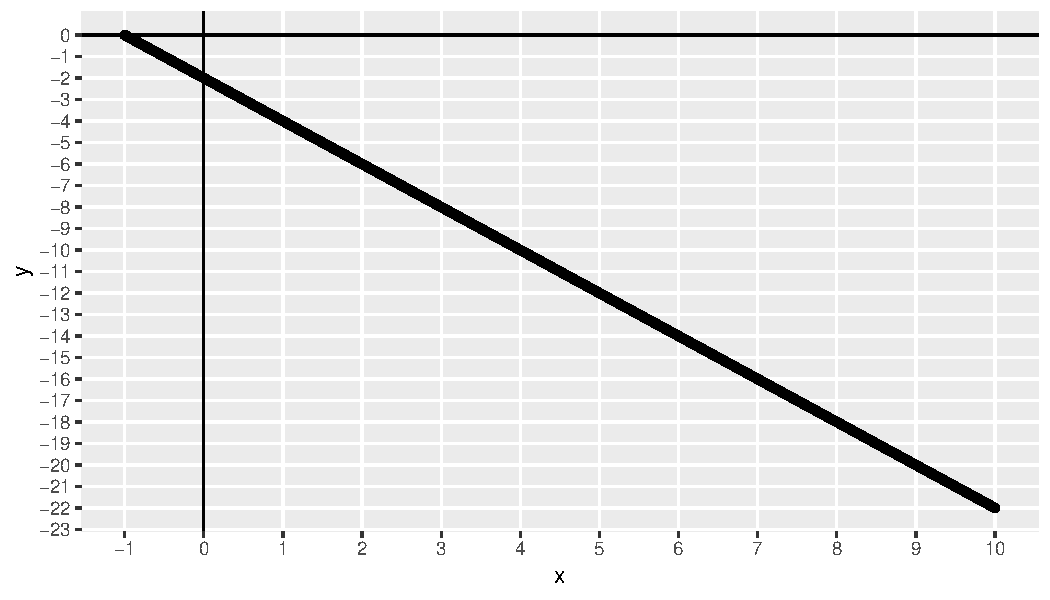
\includegraphics[width=\maxwidth]{figure/lm_3-1} 

}

\caption[Straight line with intercept -2 and slope -2]{Straight line with intercept -2 and slope -2.}\label{fig:lm_3}
\end{figure}


\end{knitrout}

\subsection{Exercises}

\begin{enumerate}
\item
For Figures \ref{fig:lm_4}, \ref{fig:lm_5} and \ref{fig:lm_6}, give the linear equations for the relationship between $x$ and $y$.


\begin{knitrout}
\definecolor{shadecolor}{rgb}{0.969, 0.969, 0.969}\color{fgcolor}\begin{figure}

{\centering 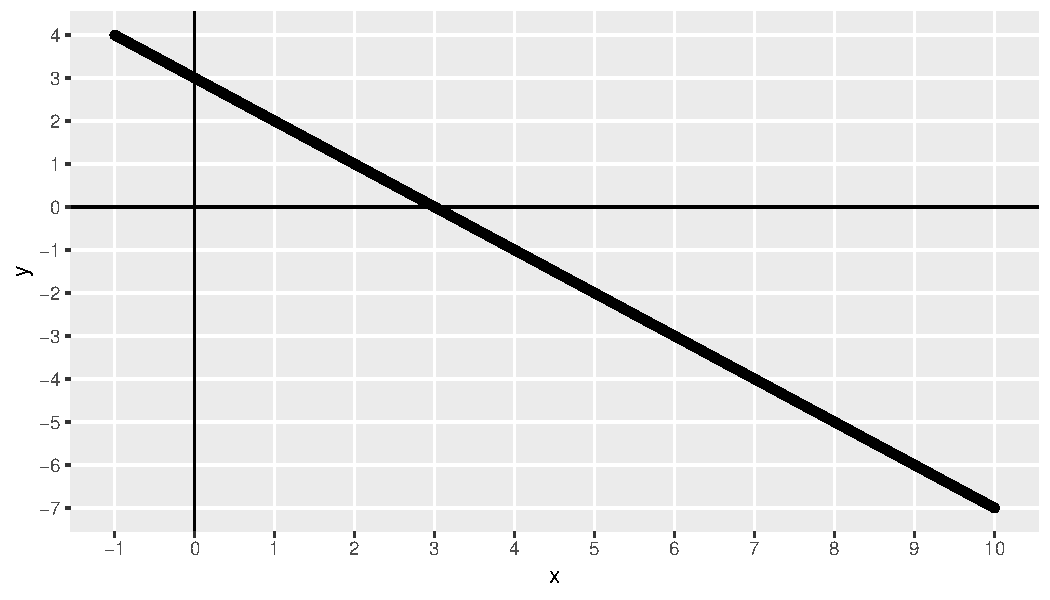
\includegraphics[width=\maxwidth]{figure/lm_4-1} 

}

\caption[Straight line example]{Straight line example.}\label{fig:lm_4}
\end{figure}


\end{knitrout}

\begin{knitrout}
\definecolor{shadecolor}{rgb}{0.969, 0.969, 0.969}\color{fgcolor}\begin{figure}

{\centering 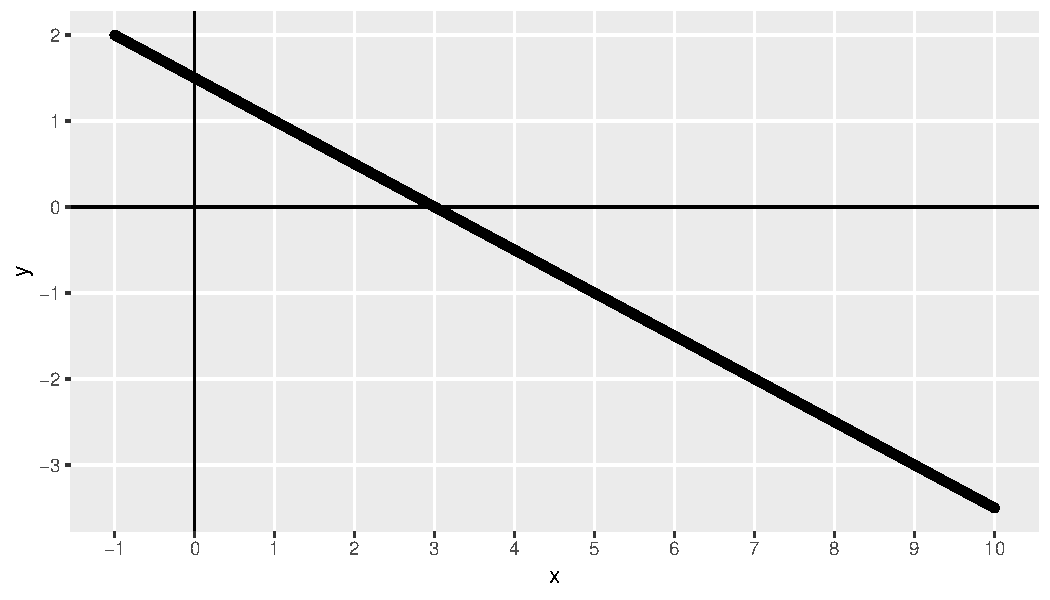
\includegraphics[width=\maxwidth]{figure/lm_5-1} 

}

\caption[Straight line example]{Straight line example.}\label{fig:lm_5}
\end{figure}


\end{knitrout}

\begin{knitrout}
\definecolor{shadecolor}{rgb}{0.969, 0.969, 0.969}\color{fgcolor}\begin{figure}

{\centering 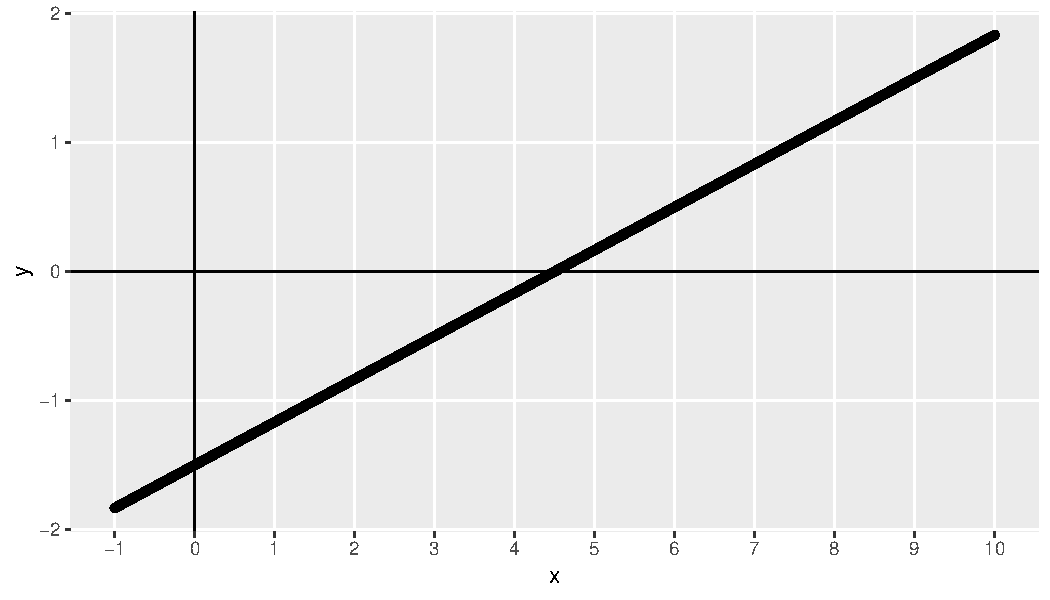
\includegraphics[width=\maxwidth]{figure/lm_6-1} 

}

\caption[Straight line example]{Straight line example.}\label{fig:lm_6}
\end{figure}


\end{knitrout}
\item
Try to sketch the straight line for the equation $y=1 - 2x$


\end{enumerate}


\subsection{Answers}

The equations are
\begin{enumerate}
\item 
\begin{equation}
y = 3 - 1 x
\end{equation}
\item
\begin{equation}
y = 1.5 - 0.5 x
\end{equation}
\item
\begin{equation}
y = -2 + 0.33 x
\end{equation}
\item
The straight line for $y=1 - 2x$ is presented in Figure \ref{fig:lm_7}.

\begin{knitrout}
\definecolor{shadecolor}{rgb}{0.969, 0.969, 0.969}\color{fgcolor}\begin{figure}

{\centering 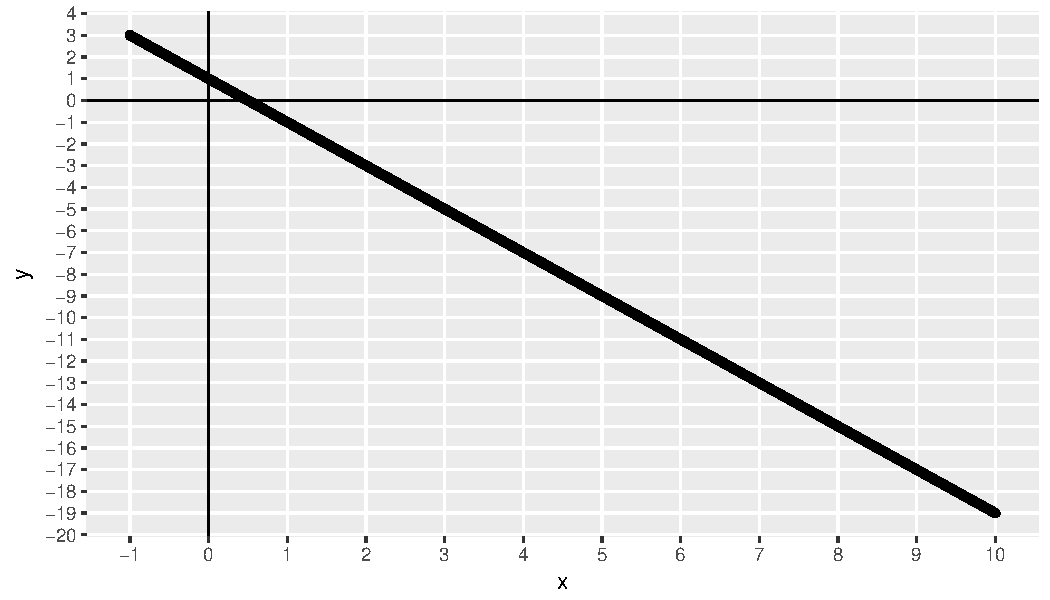
\includegraphics[width=\maxwidth]{figure/lm_7-1} 

}

\caption[Straight line with based on y=1-2x]{Straight line with based on y=1-2x.}\label{fig:lm_7}
\end{figure}


\end{knitrout}
\end{enumerate}
\section{Linear regression}

In the previous section, we saw perfect linear relationships between quantities $x$ and $y$: for each $x$-value there was only one $y$-value, and the values are all described by a straight line. Such relationships we hope to see in physics, but mostly see only in mathematics.

In social sciences we hardly ever see such perfectly linear relationships between quantities (variables). For instance, let us plot the relationship between yearly income and the amount of Euros spent on holidays. Yearly income is measured in thousands of Euros (kEuros), and money yearly spent on holidays is measured in Euros. Let us regard money spent on holidays as our dependent variable and yearly income as our independent variable (we assume money needs to be saved before it can be spent). We therefore plot yearly income on the $x$-axis (horizontal axis) and holiday spendings on the $y$-axis (vertical axis). Suppose we find the following data from 100 women between 30 and 40 years of age, plotted in Figure \ref{fig:lm_8}.


\begin{knitrout}
\definecolor{shadecolor}{rgb}{0.969, 0.969, 0.969}\color{fgcolor}\begin{figure}

{\centering 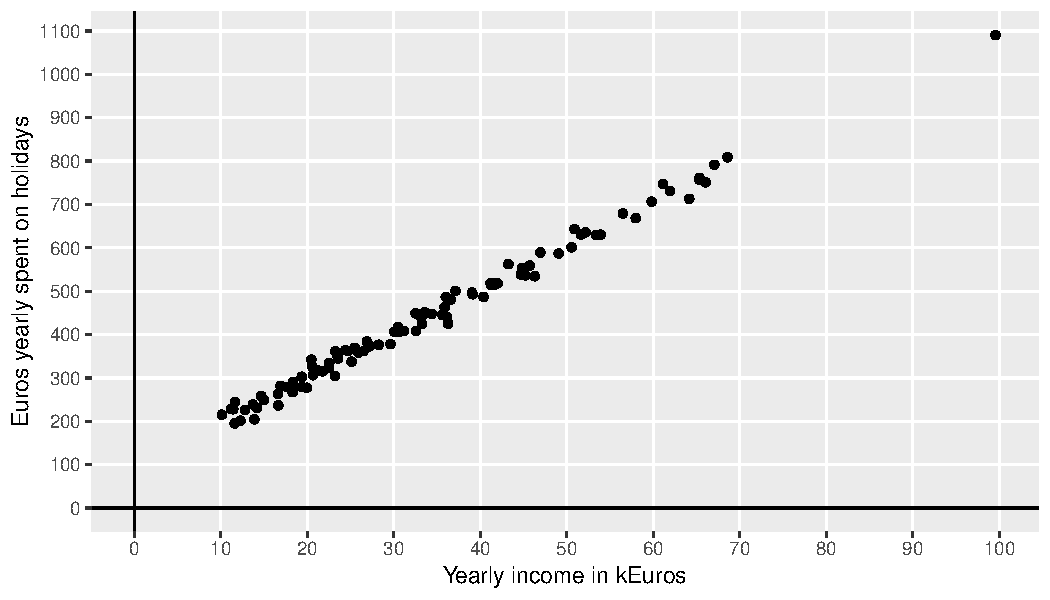
\includegraphics[width=\maxwidth]{figure/lm_8-1} 

}

\caption[Data on holiday spending]{Data on holiday spending.}\label{fig:lm_8}
\end{figure}


\end{knitrout}

In the scatterplot, we see that one woman has a yearly income of 100,000 Euros, and that she spends almost 1100 Euros per year on holidays. We also see a couple of women who earn less, between 10,000 and 20,000 Euros a year, and they spend between 200 and 300 Euros per year on holiday.

The data obviously do not form a straight line. However, we tend to think that the relationship between yearly income and holiday spending is more or less linear: there is a general linear trend such that that for every increase of 10,000 Euros in yearly income, there is an increase of about 100 Euros.

Let's plot such a straight line that represents that general trend, with a slope of 100 straight through the data points. The result is seen in Figure \ref{fig:lm_9}. We see that the line with a slope of 100 is a nice approximation of the relationship between yearly income and holiday spendings. We also see that the intercept of the line is 100.

\begin{knitrout}
\definecolor{shadecolor}{rgb}{0.969, 0.969, 0.969}\color{fgcolor}\begin{figure}

{\centering 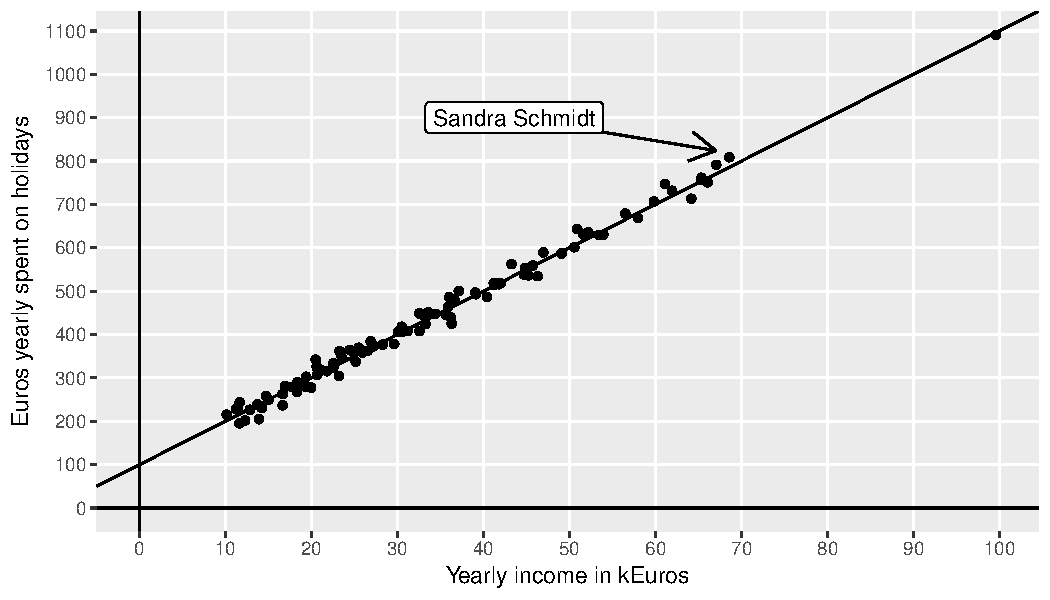
\includegraphics[width=\maxwidth]{figure/lm_9-1} 

}

\caption[Data on holiday spending with an added straight line]{Data on holiday spending with an added straight line.}\label{fig:lm_9}
\end{figure}


\end{knitrout}

Given the intercept and slope, the linear equation for the straight line approximating the relationship is

\begin{equation}
HolidaySpendings = 100 + 100 \times YearlyIncome
\end{equation}

In summary, data on two variables may not show a perfect linear relationship, but in many cases, a perfect straight line can be a very reasonable approximation of the data. Another word for a reasonable approximation of the data is a \textit{model}. Finding such a straight line to approximate the data points is called \textit{linear regression}. In this chapter we will see what method we can use to find a straight line. In linear regression we describe the behaviour of the dependent variable (the $y$-variable on the vertical axis) on the basis of the independent variable (the $x$-value on the horizontal axis) using a linear equation. We say that \textit{we regress variable $y$ on variable $x$}.




\section{Residuals}

Even though a straight line can be a good approximation of a data set consisting of two variables, it is hardly ever perfect: there are always discrepencies between what the straight line describes and what the data actually tell us.

For instance, in Figure \ref{fig:lm_9}, we see a woman, Sandra Schmidt, who makes 69 kEuros a year and who spends 809 Euros on holidays. According to the linear equation that describes the straight line, a woman that earns 69 kEuros a year would spend $100 + 100 * 69= 786$ Euros on holidays. The discrepency between the actual amount spent and the amount prescribed by the linear equation equals $809-786=23$ Euros. This difference is rather small and the same holds for all the other women in this data set. Such discrepencies between the actual amount spent and the amount as prescribed or predicted by the straight line are called \textit{residuals} or \textit{errors}. The residual (or error) is the difference between a certain data point (the \textit{actual} value) and what the linear equation predicts.


% Using the linear equation, we could predict holiday spendings even for yearly incomes that are not in the data set. For instance, in this data set there is no woman with an income of 80,000, but still we can use the linear equation with a prediction that such a woman would probably spend around $100+100\times 80= 8100$ Euros.


Let us look at another fictitious data set where the residuals (errors) are a bit larger. Figure \ref{fig:lm_10} shows the relationship between variables $x$ and $y$. The dots are the actual data points and the blue straight line is an approximation of the actual relationship. The residuals are also visualized: sometimes the observed $y$-value is greater than the predicted $y$-value (dots above the line) and sometimes the oberved $y$-value is smaller than the predicted $y$-value (dots below the line). Let's denote the predicted $y$-value (the value of $y$ predicted by the blue line) as $\hat{y}$ (pronounced as y-hat), then we can define a residual or error as the discrepency between the observed $y$ and $\hat{y}$:

\begin{equation}
e = y - \hat{y}
\end{equation}

where $e$ stands for the error (residual).


\begin{knitrout}
\definecolor{shadecolor}{rgb}{0.969, 0.969, 0.969}\color{fgcolor}\begin{figure}

{\centering 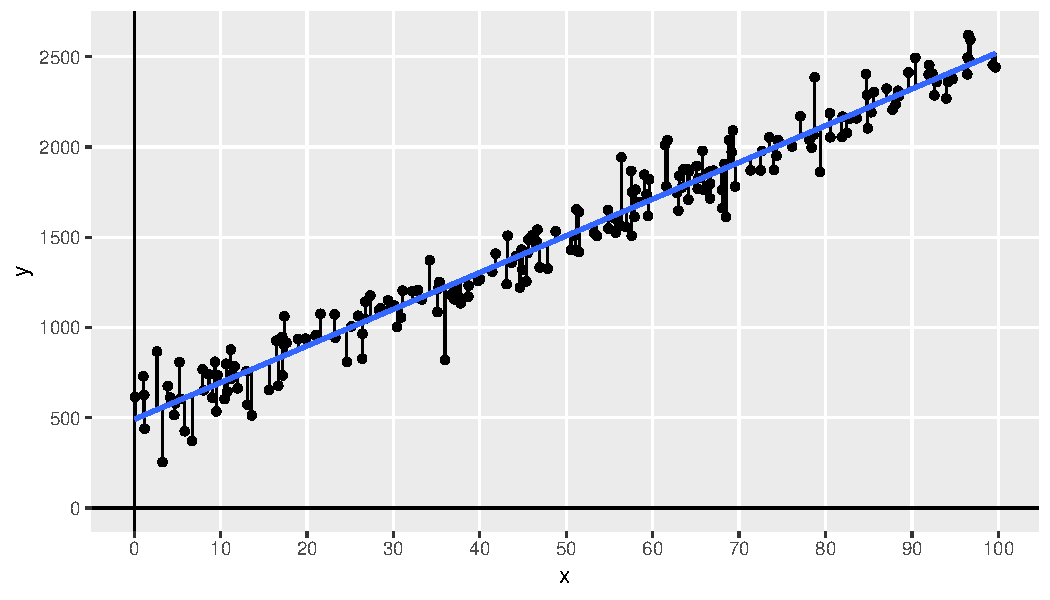
\includegraphics[width=\maxwidth]{figure/lm_10-1} 

}

\caption[Data on variables x and y with an added straight line]{Data on variables x and y with an added straight line.}\label{fig:lm_10}
\end{figure}


\end{knitrout}

If we compute residual $e$ for every $y$-value in the data set, we can plot them using a histogram, as displayed in Figure \ref{fig:lm_11}. We see that the residuals are on average 0, and that the histogram has the shape of a normal distribution, more or less. Such normally-shaped distributions of residuals we see often in research. Here, the residuals show a normal distribution with mean 0 and variance of 13336 (a standard deviation of 115).


\begin{knitrout}
\definecolor{shadecolor}{rgb}{0.969, 0.969, 0.969}\color{fgcolor}\begin{figure}

{\centering 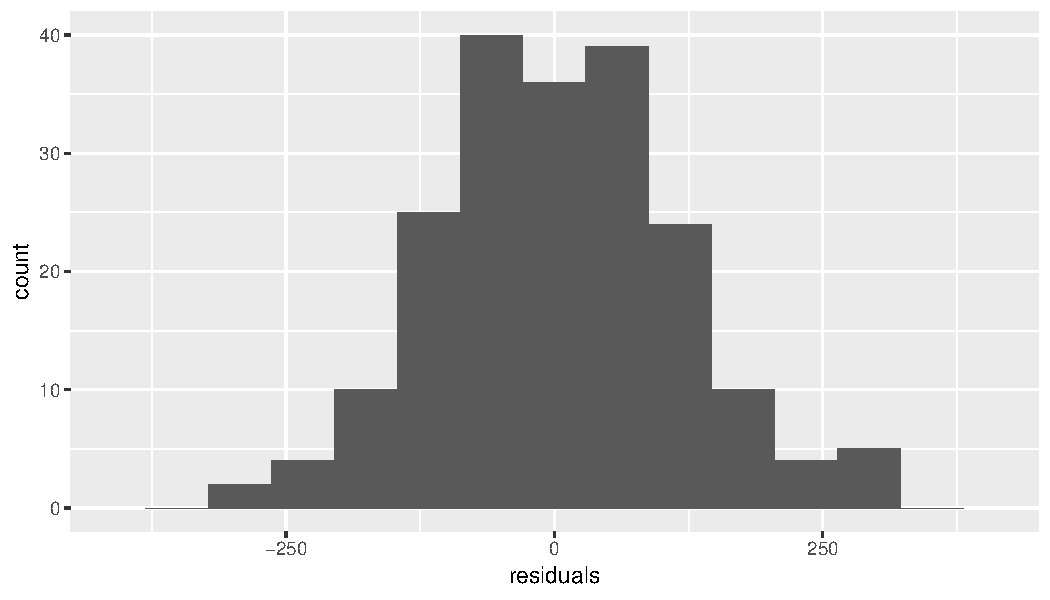
\includegraphics[width=\maxwidth]{figure/lm_11-1} 

}

\caption[Histogram of the residuals (errors)]{Histogram of the residuals (errors).}\label{fig:lm_11}
\end{figure}


\end{knitrout}


\section{Least squares regression lines}


You may ask yourself how to draw a straight line through the data points: How do you decide the exact slope and the exact intercept? And what if you don't want to draw the data points and the straight line by hand? That can be quite cumbersome if you have more than 2000 data points to plot!

First, because we are lazy, we always use a computer to draw the data points and the regression line. Second, since we could draw many different straight lines through a scatter of points, we need a criterion to determine a nice combination of intercept and slope. With such a criterion we can then let the computer determine the straight line with its equation for us.

The criterion that we use in this chapter is called Least Squares, or Ordinary Least Squares (OLS). To explain the Least Squares principle, look again at Figure \ref{fig:lm_10} where we see both small and large residuals. About half of them are positive (above the blue line) and half of them are negative (below the blue line).

The most reasonable idea is to draw a straight line that is more or less in the middle of the $y$-values, in other words, with about half of the residuals positive and about half of them negative. Or perhaps we could say that on average, the residuals should be 0. A third way of saying the same thing is that the sum of the residuals should be equal to 0.

However, the criterion that all residuals should sum to 0 is not sufficient. In Figure \ref{fig:lm_12} we see a straight line with a slope of 0 where all residuals sum to 0. However, this regression line does not make intuitive sense: it does not describe the structure in the data very well. Moreover, we see that the residuals are much larger than in Figure \ref{fig:lm_10}.

\begin{knitrout}
\definecolor{shadecolor}{rgb}{0.969, 0.969, 0.969}\color{fgcolor}\begin{figure}

{\centering 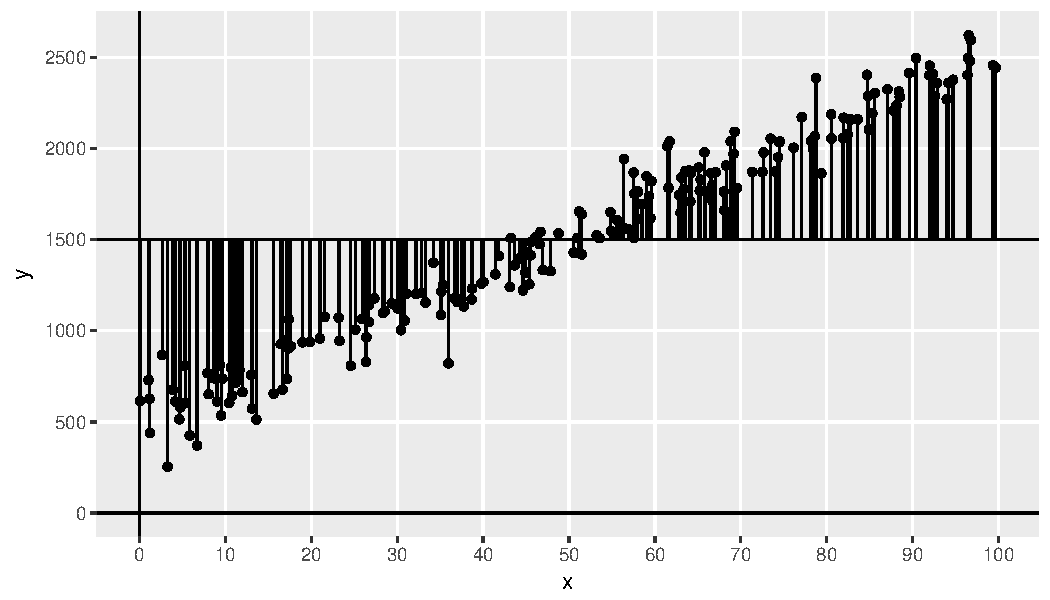
\includegraphics[width=\maxwidth]{figure/lm_12-1} 

}

\caption[Data on variables x and y with an added straight line]{Data on variables x and y with an added straight line. The sum of the residuals equals 0.}\label{fig:lm_12}
\end{figure}


\end{knitrout}

We therefore need a second criterion to find a nice straight line. We want the residuals to sum to 0, but also want the residuals to be as small as possible: the descrepencies between what the linear equation predicts (the $\hat{y}$-values) and the actual $y$-values should be as small as possible.

So now we have two criteria: we want the sum of the residuals to be 0 (about half of them negative, half of them positive), and we want the residuals to be as small as possible. We can achieve both of these when we use as our criterion the idea that the sum of the \textit{squared} residuals be as small as possible. Recall from Chapter 1 that the sum of the squared deviations from the mean is actually the variance. So if the sum of the squared residuals is as small as possible, we know that the variance of the residuals is as small as possible. Thus, as our criterion we can use the regression line for which the squared differences between predicted and observed $y$-values are as small as possible.

Figure \ref{fig:lm_13} shows three different regression lines for the same data set. Figure \ref{fig:lm_14} shows the respective distributions of the residuals. For the first line, we see that the residuals sum to 0, for the residuals are on average 0 (the red vertical line). However, we see quite large residuals. The residuals for the second line are smaller: we see very small positive residuals, but the negative residuals are still quite large. We also see that the residuals do not sum to 0. For the third line, we see both criteria optimized: the sum of the residuals is zero and the residuals are all very small. We see that for regression line 3, the sum of squared residuals is at its minimum value.



\begin{knitrout}
\definecolor{shadecolor}{rgb}{0.969, 0.969, 0.969}\color{fgcolor}\begin{figure}

{\centering 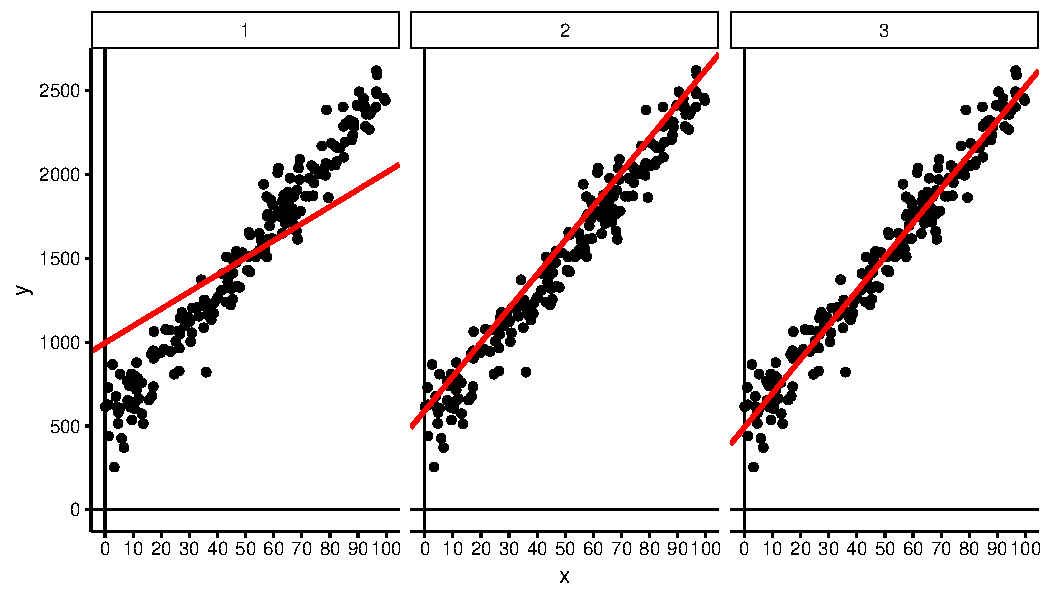
\includegraphics[width=\maxwidth]{figure/lm_13-1} 

}

\caption[Three times the same data set, but with different regression lines]{Three times the same data set, but with different regression lines.}\label{fig:lm_13}
\end{figure}


\end{knitrout}

\begin{knitrout}
\definecolor{shadecolor}{rgb}{0.969, 0.969, 0.969}\color{fgcolor}\begin{figure}

{\centering 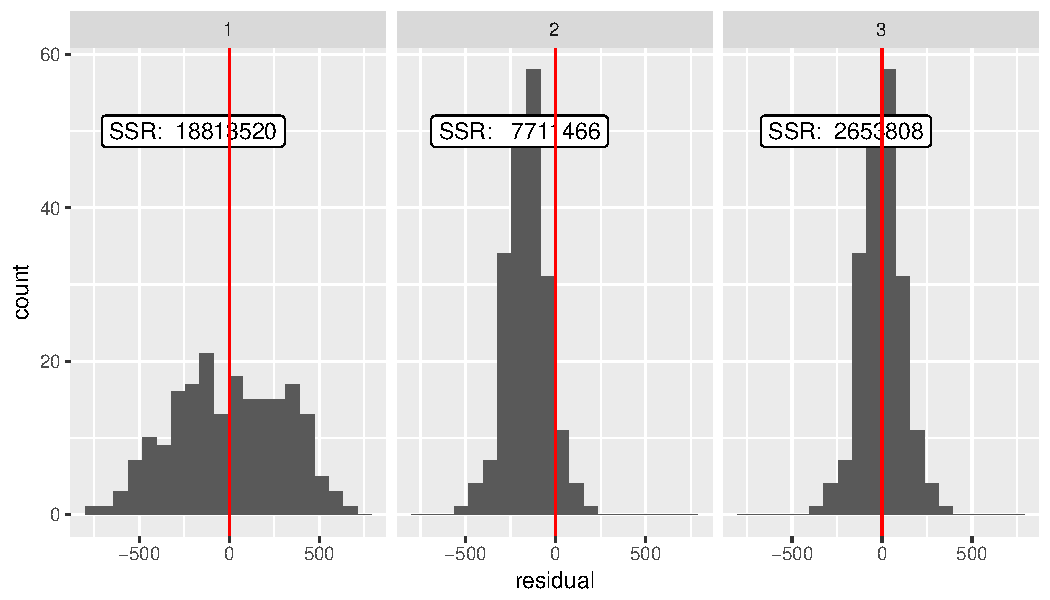
\includegraphics[width=\maxwidth]{figure/lm_14-1} 

}

\caption[Histogram of the residuals (errors) for three different regression lines, and the respective sums of squared residuals (SSR)]{Histogram of the residuals (errors) for three different regression lines, and the respective sums of squared residuals (SSR).}\label{fig:lm_14}
\end{figure}


\end{knitrout}

In summary, when we want to have a straight line that describes our data best, we'd like a line such that the residuals are on average 0 (i.e, sum to 0), and where we see the smallest residuals possible. We reach these criteria when we use the line in such a way that we have the lowest value for the sum of the squared residuals possible. This line is therefore called the least squares or OLS regression line. It turns out that this optimal regression slope can be found by a relatively simple computation using matrix algebra. In daily life, we do not do this by hand but let computers compute it for us, with software like for instance SPSS or R.


\subsection{Exercises}

\begin{enumerate}



% latex table generated in R 3.5.0 by xtable 1.8-2 package
% Mon Jan 21 16:42:18 2019
\begin{table}[ht]
\centering
\caption{Home prices.} 
\label{tab:lm_15}
\begin{tabular}{rrlll}
  \hline
Area & Price & PredictedPrice & Residual & SquaredResidual \\ 
  \hline
56.00 & 165.00 &   &   &   \\ 
  101.00 & 180.00 &   &   &   \\ 
  67.00 & 115.00 &   &   &   \\ 
  109.00 & 164.00 &   &   &   \\ 
  115.00 & 175.00 &   &   &   \\ 
  34.00 & 135.00 &   &   &   \\ 
   \hline
\end{tabular}
\end{table}


\item In Table \ref{tab:lm_15} you find a small data set on the price of homes with dependent variable price in kEuros and independent variable area in square meters. The least squares regression equation turns out to be $price = 106.9386105+ 0.603671\times area$. Add a third column with the expected prices based on the regression equation ($\hat{y}$. Put the difference between the observed price and the expected price in the fourth column ($e$). Then compute the squared residuals and put those in the fifth column ($e^2)$. Take the sum of the squared residuals: How large is sum of the squared residuals?


\item See website \url{https://gallery.shinyapps.io/simple_regression/}, try to find the Least Squares regression line for the given data set by changing both intercept and slope. How large is the sum of the squared residuals for that optimal regression line?


\item Do this exercice with one or more of your fellow students. Look at the data set plotted in Figure \ref{fig:lm_16}. Try to find the regression line with the lowest sum of squared residuals possible.

\begin{knitrout}
\definecolor{shadecolor}{rgb}{0.969, 0.969, 0.969}\color{fgcolor}\begin{figure}

{\centering 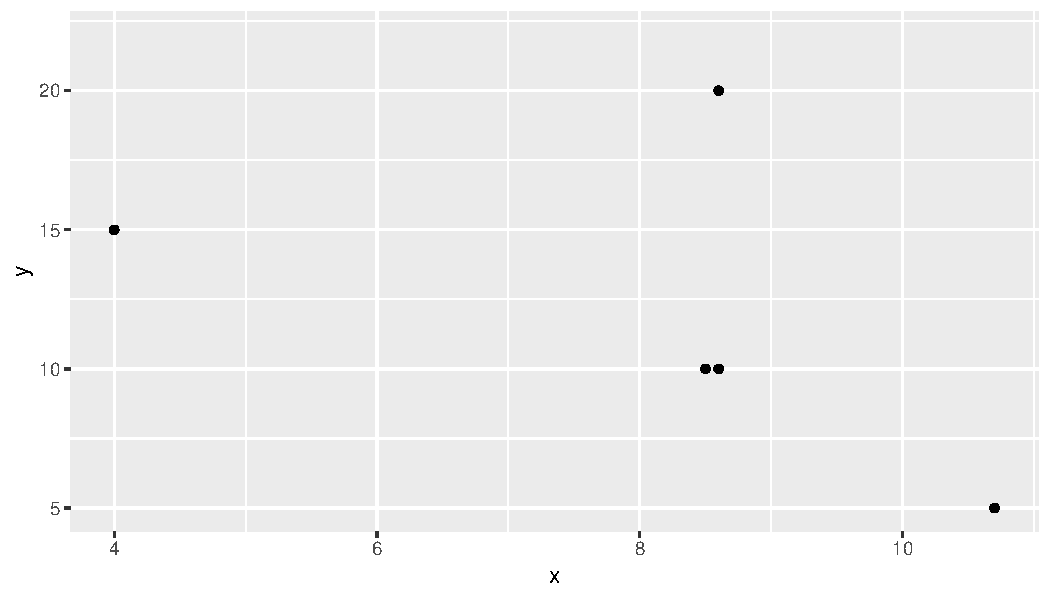
\includegraphics[width=\maxwidth]{figure/lm_16-1} 

}

\caption[Plot of housing data]{Plot of housing data.}\label{fig:lm_16}
\end{figure}


\end{knitrout}


\end{enumerate}

\subsection{Answers}


\begin{enumerate}

\item The predicted prices, the residuals and the squared residuals are displayed in Table \ref{tab:lm_17}. The sum of the squared residuals equals 2397.4189795.

% latex table generated in R 3.5.0 by xtable 1.8-2 package
% Mon Jan 21 16:42:19 2019
\begin{table}[ht]
\centering
\caption{Home prices.} 
\label{tab:lm_17}
\begin{tabular}{rrrrr}
  \hline
Area & Price & PredictedPrice & Residual & SquaredResidual \\ 
  \hline
56.00 & 165.00 & 140.74 & 24.26 & 588.34 \\ 
  101.00 & 180.00 & 167.91 & 12.09 & 146.18 \\ 
  67.00 & 115.00 & 147.38 & -32.38 & 1048.76 \\ 
  109.00 & 164.00 & 172.74 & -8.74 & 76.37 \\ 
  115.00 & 175.00 & 176.36 & -1.36 & 1.85 \\ 
  34.00 & 135.00 & 127.46 & 7.54 & 56.80 \\ 
   \hline
\end{tabular}
\end{table}

\item

\item The lowest sum of squared residuals is 97. This is the sum that you get with intercept 21.4 and slope -1.2.

\end{enumerate}







\section{Pearson correlation}

For any set of two quantitative variables, we can determine the least squares regression line. However, it depends on the data set how well that regression line describes the data. Figure \ref{fig:lm_18} shows two different data sets on variables $x$ and $y$. Both plots also show the least squares regression line, and they both turn out to be exactly the same: $y=100+10x$.

\begin{knitrout}
\definecolor{shadecolor}{rgb}{0.969, 0.969, 0.969}\color{fgcolor}\begin{figure}

{\centering 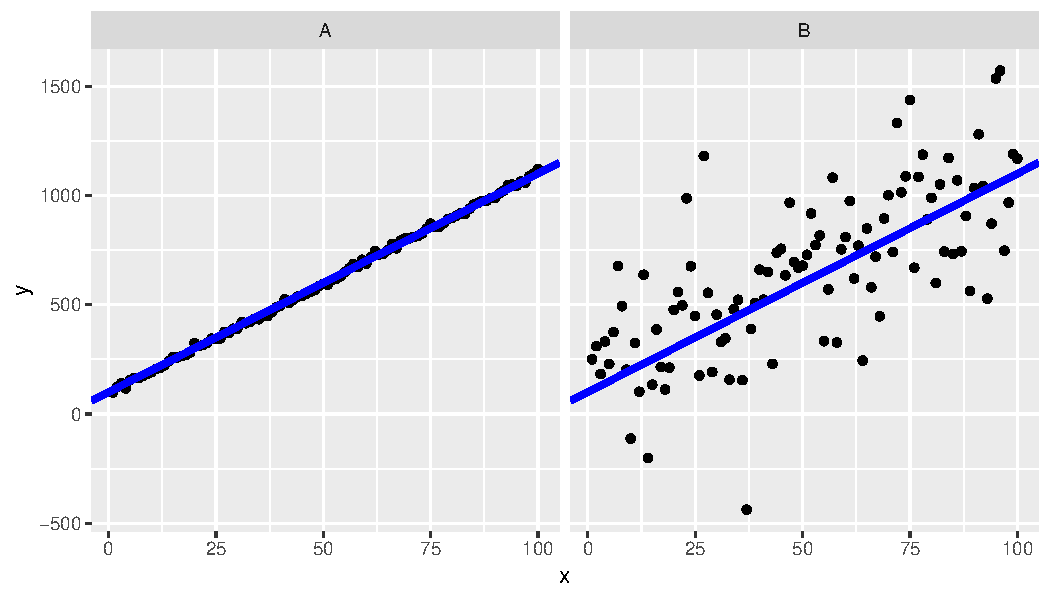
\includegraphics[width=\maxwidth]{figure/lm_18-1} 

}

\caption[Plot of housing data]{Plot of housing data.}\label{fig:lm_18}
\end{figure}


\end{knitrout}


We see that the regression line describes data set A very well (left panel): the observed dots are very close to the line, which means that the residuals are very small. The regression line does a worse job for data set B (right panel) since there are quite large discrepencies between the observed $y$-values and the predicted $y$-values. Put differently, the regression equation can be used to predict $y$-values in data set A very well, almost without error, whereas the regression line cannot be used to predict $y$-values in data set B very precisely. The regression line is also the least squares regression line for data set B, so any improvement by choosing another slope or intercept is not possible.

Francis Galton was the first to think about how to quantify this difference in the ability of a regression line to predict the dependent variable. Karl Pearson later worked on this measure so that it became to be called Pearson's correlation coefficient. It is a standardized measure, so that it can be used to compare different data sets.

In order to get to Pearson's correlation coefficient, you first need to standardize both the independent variable, $x$, and the dependent variable, $y$. You standardize scores by taking their values, subtract the mean from them, and divide by the standard deviation (see Chapter 1). So, in order to obtain a standardized $x$-value we compute $Z_x$,

\begin{equation}
Z_x = \frac{x- \bar{x}}{\sigma_x}
\end{equation}

and in order to obtain a standardized $y$-value we compute $Z_y$,

\begin{equation}
Z_y = \frac{y- \bar{y}}{\sigma_y}.
\end{equation}



\begin{knitrout}
\definecolor{shadecolor}{rgb}{0.969, 0.969, 0.969}\color{fgcolor}\begin{figure}

{\centering 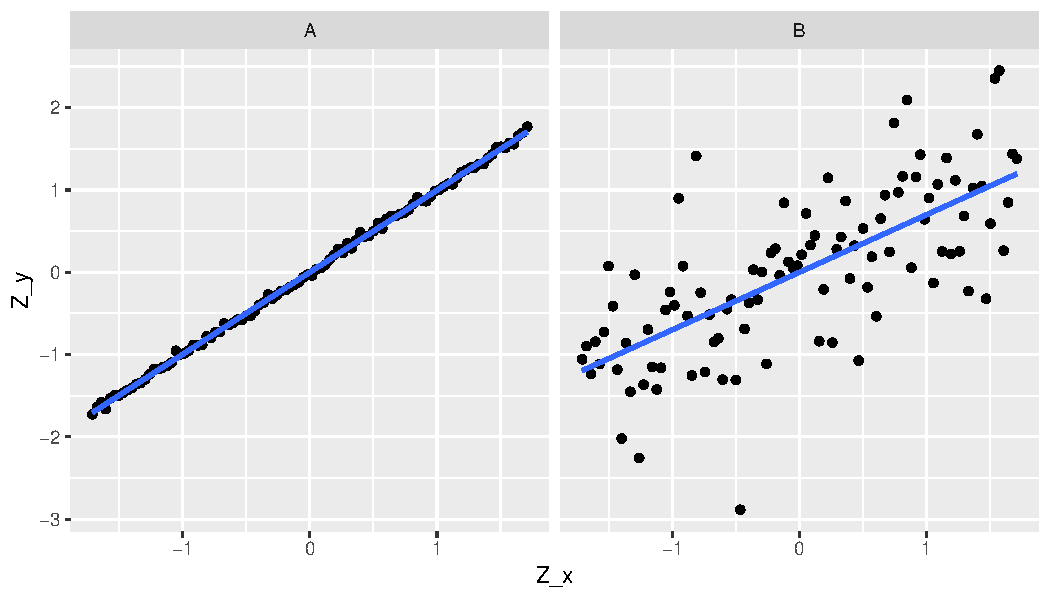
\includegraphics[width=\maxwidth]{figure/lm_19-1} 

}

\caption[Plot of housing data]{Plot of housing data.}\label{fig:lm_19}
\end{figure}


\end{knitrout}

Let's do this both for data set A and data set B, and plot the standardized scores, see Figure \ref{fig:lm_19}. If we then plot the least squares regression lines for the standardized values, we obtain different equations. For both data sets, the intercept is 0 because by standardizing the scores, the means become 0. But the slopes are different: in data set A, the slope is 0.997 and in data set B, the slope is 0.699.

\begin{eqnarray}
Z_y = 0 + 0.997Z_x=0.997Z_x \\
Z_y = 0 + 0.699Z_x=0.699Z_x
\end{eqnarray}


These two slopes, the slope for the regression of standardized $y$-values on standardized $x$-values, are the correlation coefficients for data sets A and B, respectively. For obvious reasons, the correlation is sometimes also referred to as the \textit{standardized slope coefficient}.

Correlation stands for the \textit{co-relation} between two variables. It tells you how strongly one variable can be predicted from the other. The correlation is bi-directional: the correlation between $y$ and $x$ is the same as the correlation between $x$ and $y$. For instance in Figure \ref{fig:lm_19}, if we would have put the $Z_x$-variable on the $Z_y$-axis, and the $Z_y$-variable on the $Z_x$-axis, the slopes would be exactly the same. This is true because the variances of the $y$ and $x$-variables are equal after standardization (both variances equal to 1).

Since a slope can be negative, a correlation can be negative too. Furthermore, a correlation is always between -1 and 1. Look at Figure \ref{fig:lm_19}: the correlation between $x$ and $y$ is 0.997. The dots are almost on a straight line. If the dots would all be exactly on the straight line, the correlation would be 1.

\begin{knitrout}
\definecolor{shadecolor}{rgb}{0.969, 0.969, 0.969}\color{fgcolor}\begin{figure}

{\centering 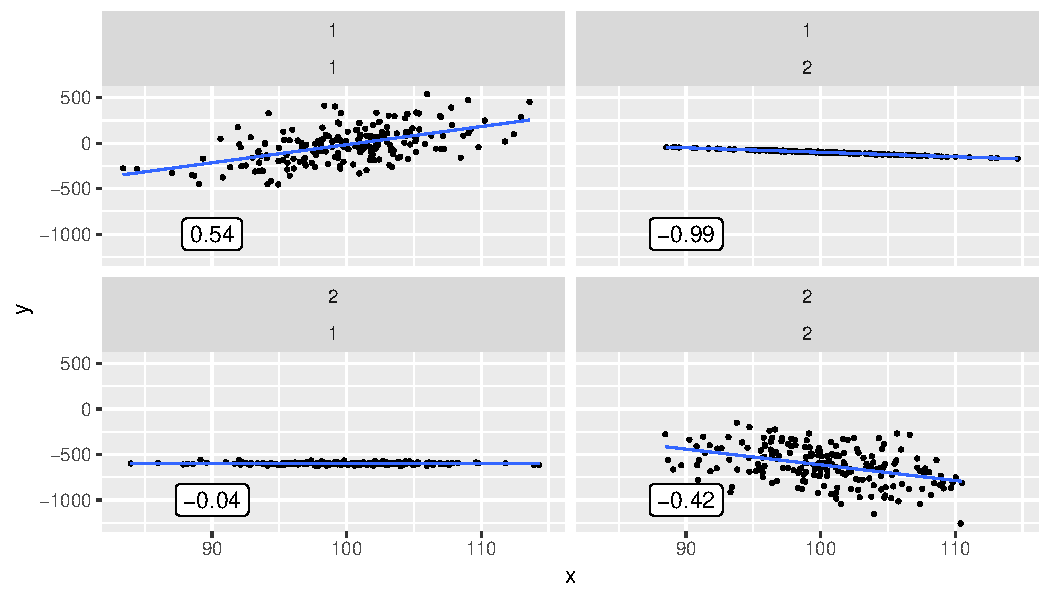
\includegraphics[width=\maxwidth]{figure/lm_20-1} 

}

\caption[Various plots showing different correlations between variables x and y]{Various plots showing different correlations between variables x and y.}\label{fig:lm_20}
\end{figure}


\end{knitrout}


Figure \ref{fig:lm_20} shows a number of scatterplots of $x$ and $y$ with different correlations. Note that if dots are very close to the regression line, the correlation can still be close to 0. If the slope is 0 (bottom-left panel), then one variable cannot be predicted from the other variable, hence the correlation is 0, too.

In summary, the correlation coefficient indicates how well one variable can be predicted from the other variable. It is the slope of the regression line if both variables are standardized. If prediction is not possible (when the regression slope is 0), the correlation is 0, too. If the prediction is perfect, without errors (no residuals) and with a slope unequal to 0, then the correlation is either -1 or +1, depending on the sign of the slope.

\section{Covariance}

The correlation is a standardized measure for how much two variables co-relate. There exists also an unstandardized measure for how much two variables co-relate: the \textit{covariance}. The correlation is the slope when two variables have each variance 1. When you multiply the correlation by a number indicating the variances of the two variables, you get the covariance. This number is the product of the two respective standard deviations.

The covariance between variables $x$ and $y$, Cov(x,y) can be computed as:


\begin{equation}
Cov(x,y)= Cor(x,y) \times \sigma_x \sigma_y
\end{equation}

For example, if the variance of $x$ equals 49 and the variance of $y$ equals 25, then the respective standard deviations are 7 and 5. If the correlation between $x$ and $y$ equals 0.5, then the covariance between $x$ and $y$ is equal to $0.5 \times 7 \times 5 = 17.5$.

Similar to correlation, the covariance of two variables indicates by how much they co-vary. For instance, if the variance of $x$ is 3 and the variance of $y$ is 5, then a covariance of 2 indicates that $x$ and $y$ co-vary: if $x$ increases by a certain amount, $y$ also increases. If you want to know how many standard deviations $y$ increases if $x$ increases with one standard deviation, you can turn the covariance into a correlation by dividing the covariance by the respective standard deviations.

\begin{equation}
Cor(x,y)= \frac{Cov(x,y)} { \sigma_x \sigma_y}= \frac{2} { \sqrt{3} \sqrt{5}}=0.52
\end{equation}

Similar to correlations and slopes, covariances can also be negative.


\subsection{Exercises}

\begin{enumerate}

\item The correlation between brain size and intelligence in 9-year old children equals 0.30. Suppose the variance in brain size equals 45 and the variance in intelligence 225. Compute the covariance.



\item The covariance between intelligence and extraversion equals 1. The variance of intelligence is 225 and the variance of extraversion is 9. What is the correlation?




\item Suppose the correlation between intelligence and extraversion is 0.10. What does this mean?



\item Suppose the correlation between intelligence and extraversion is -0.05. What does this mean?




\item Suppose the correlation between intelligence and extraversion is 0.30. What is the regression slope if the variance of intelligence is 225 and the variance of extraversion is 9?



\end{enumerate}

\subsection{Answers}

\begin{enumerate}

\item

\begin{equation}
Cov(x,y)= Cor(x,y) \times \sigma_x \sigma_y= 0.30 \times \sqrt{45}\times \sqrt{225}=30
\end{equation}



\item

\begin{equation}
Cor(x,y)= \frac{Cov(x,y)} { \sigma_x \sigma_y}= \frac{1} { \sqrt{225} \sqrt{9}}=0.02
\end{equation}

\item
If you increase intelligence by 1 standard deviation, then extraversion increases with a tenth of a standard deviation.

\item
If you increase intelligence by 1 standard deviation, then extraversion increases with 0.05 standard deviations.

\item
The correlation is 0.30, so if you increase intelligence by one standard deviation (which is $\sqrt{225}=15$), extraversion increases by 0.30 standard deviations (which equals $0.30 \times \sqrt{9}=0.90$). Therefore, if you increase intelligence by 15 points, you increase extraversion by 0.90 points. Thus if you increase intelligence by 1 point, you increase extraversion by $0.90/15=0.06$ points. The slope for the regression of extraversion on intelligence is therefore 0.06.


\end{enumerate}


\section{Regression using SPSS}

\begin{knitrout}
\definecolor{shadecolor}{rgb}{0.969, 0.969, 0.969}\color{fgcolor}\begin{figure}

{\centering 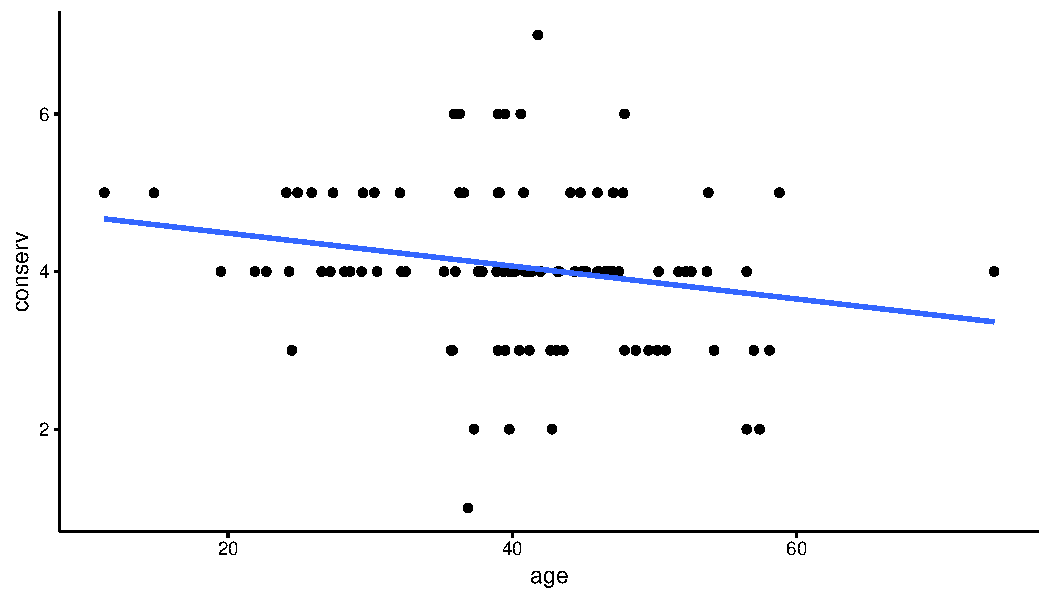
\includegraphics[width=\maxwidth]{figure/lm_22-1} 

}

\caption[Imaginary data set on age and conservatism scores in 102 men]{Imaginary data set on age and conservatism scores in 102 men.}\label{fig:lm_22}
\end{figure}


\end{knitrout}

Figure \ref{fig:lm_22} shows an imaginary data set on age and conservatism scores on a 7-point scale in 102 men. The blue line is the least squares regression line. This line can be found with SPSS using the following UNIANOVA syntax:

\begin{verbatim}
UNIANOVA conserv WITH age
/PRINT parameter.
\end{verbatim}

In the syntax we first indicate the dependent variable (the one that we want to explain, which is in this case \textbf{conserv}), and then we indicate that we want to explain this variable with the independent variable \textbf{age}. In the next line we indicate that we want to see the intercept and slope parameters in the output.

SPSS will then show two tables. The first table will be discussed in later chapters. For now, we only look for the table with the Parameter Estimates. Figure \ref{fig:simple} shows that table. It shows that the dependent variable is indeed \textbf{conserv}, and that there are two parameters in our regression model: an intercept and a slope parameter for the variable \textbf{age}. In the column with $B$ we find the values for these parameters. The intercept has the value 4.904 (when rounded to 3 decimals) and the slope has the value -0.021. Thus, with this output, the linear equation for the regression line can be filled in:

\begin{equation}
conserv = 4.904 - 0.021 \times age + e
\end{equation}

With this equation we can predict values for conservatism for ages that are not even in the data set displayed in Figure \ref{fig:lm_22}. For instance, that plot does not show a man of age 70, but on the basis of the linear equation, the best bet would be that such a man would have a conservatism score of $4.904 - 0.021 \times 70= 3.434$.


\begin{figure}[h]
    \begin{center}
       \includegraphics[scale=0.8, trim={0cm 26cm 0cm 0cm}]{/Users/stephanievandenberg/Dropbox/Statistiek_Onderwijs/Data" "Analysis/spss" "examples"  "linear" "model/simple.pdf}
    \end{center}
    \caption{SPSS output of a simple regression.}
    \label{fig:simple}
\end{figure}




\section{Linear models}

By performing a regression analysis of $y$ on $x$, we try to predict the $y$-value from a given $x$-value on the basis of a linear equation. We try to find an intercept and a slope for that linear equation such that our prediction is 'best'. We define 'best' as the linear equation for wich we see the lowest possible value for the sum of the squared residuals (least squares principle).

Thus, the predicted value of $y$ ($\hat{y}$) can be computed by the linear equation

\begin{equation}
\hat{y}= b_0 + b_1 x
\end{equation}

In reality, the predicted values of $y$ always deviate from the observed values of $y$. So, there is always an error $e$ that is the difference between $\hat{y}$ and $y$. Thus we have for the observed values of $y$

\begin{equation}
y = \hat{y} + e = b_0 + b_1 x + e
\end{equation}

Typically, we assume that the residuals $e$ have a normal distribution with a mean of 0 and a variance of that is often unknown but that we denote by $\sigma^2_e$. Such a normal distribution is denoted by $N(\mu,\sigma^2)$. Taking the linear equation and the normally distributed residuals together, we have \textit{a linear model} for the two variables $x$ and $y$.


\begin{eqnarray}
y = b_0 + b_1 x + e \\
e \sim N(0,\sigma^2_e)
\end{eqnarray}


The linear model that we see here is generally known as the simple regression model: a linear model for one dependent variable, an intercept, only one slope for one (hence 'simple')  independent variable,  and normally distributed residuals. In the remainder of this book, we will see a great variety of linear models: with one or more independent variables, with numeric or with categorical independent variables, and with numeric or with categorical dependent variables. All these models can be seen as extensions of this basic linear regression model. They all aim to predict as best as possible one dependent variable from one or more independent variables. % simple regression





\chapter{Inference I: random samples, standard errors and confidence intervals}\label{chap:confidence}

In Chapter \ref{chap:simple} on simple regression we saw how a linear equation can describe a data set: the linear equation describes the behaviour of one variable, the dependent variable, on the basis of one other variable, the independent variable. Sometimes we are indeed interested in the relationship between two variables in one given data set. For instance, a teacher wants to know whether her exam gradings in her class of last year predict how well her students do in a second course a year later.

\begin{knitrout}
\definecolor{shadecolor}{rgb}{0.969, 0.969, 0.969}\color{fgcolor}\begin{figure}

{\centering 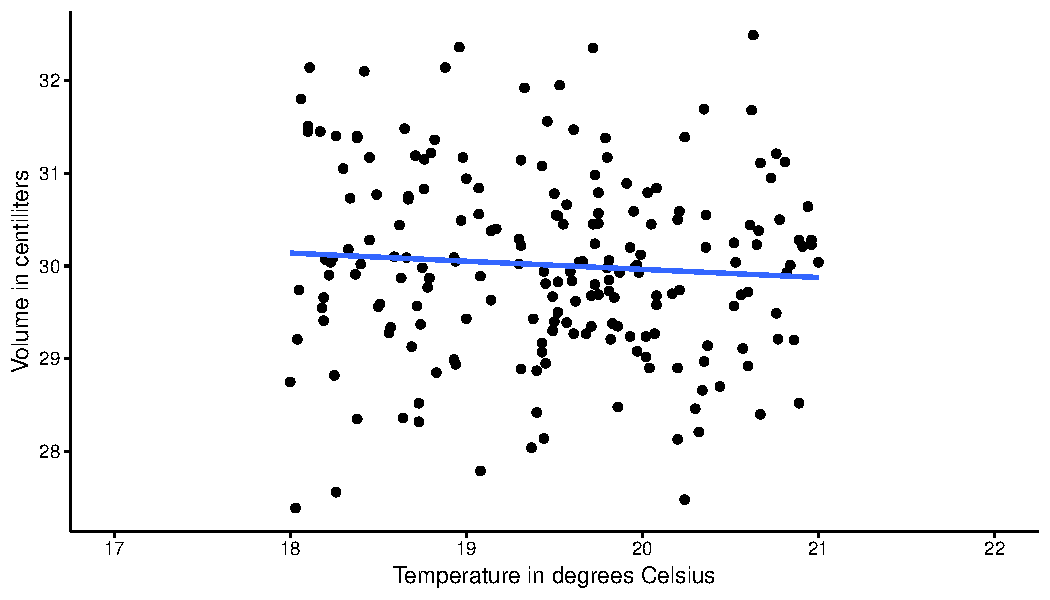
\includegraphics[width=\maxwidth]{figure/inf_0-1} 

}

\caption[The relationship between temperature and volume in a sample of 200 bottles]{The relationship between temperature and volume in a sample of 200 bottles.}\label{fig:inf_0}
\end{figure}


\end{knitrout}


But very often, researchers are not interested in the relationships between variables in one data set, but interested in the relationship between variables in general, not limited to only the observed data. For example, a researcher would like to know what the relationship is between the temperature in a brewery and the volume of beer that goes into the beer bottles. In order to study the effect of temperature on volume, the researcher measures the volume of beer in a limited collection of 200 bottles at 20 degrees Celsius and determines from log files the temperature in the factory during production for each measured bottle. The linear equation might be $volume = 31.72 -0.088 \times temp + e$, see Figure \ref{fig:inf_0}. But the question is what the equation would be if the researcher had used information about \textit{all} bottles produced in the same factory.



In other words, we may know about the linear relationship between temperature and volume in a \textit{sample} of bottles, but we might really be interested to know what the relationship would look like \textit{had we been able to measure the volume in all bottles}.


\section{Population data and sample data}

In the beer bottle example above, the volume of beer was measured in a total of 200 bottles. Let's do a thought experiment. Suppose we could have access to volume data about all bottles of beer on all days where the factory was operating, including information about the temperature for each day of production. Suppose that the total number of bottles produced is 80,000 bottles. When we plot the volume of each bottle against the temperature of the factory we get the scatterplot in Figure \ref{fig:inf_1}.


\begin{knitrout}
\definecolor{shadecolor}{rgb}{0.969, 0.969, 0.969}\color{fgcolor}\begin{figure}

{\centering 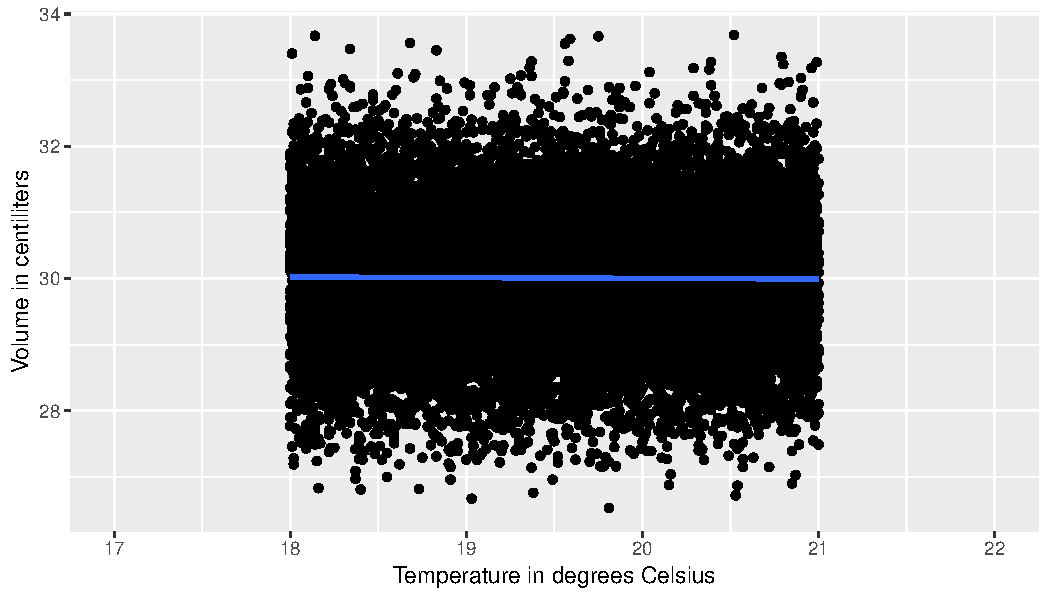
\includegraphics[width=\maxwidth]{figure/inf_1-1} 

}

\caption[The relationship between temperature and volume in all 80,000 bottles]{The relationship between temperature and volume in all 80,000 bottles.}\label{fig:inf_1}
\end{figure}


\end{knitrout}


In our thought experiment, we could determine the regression equation using all bottles that were produced: all 80,000 of them. We then find the blue regression line displayed in Figure \ref{fig:inf_1}. Its equation is $Volume = 29.98 + 0.001 \times temp$.


In the data example above, data was only collected on 200 bottles. These bottles were randomly selected\footnote{Random selection means that each of the 80,000 bottles had an equal probability to end up in this sample of 200 bottles.}: there were many more bottles but we could measure only a limited number of them. This explains why the regression equation based on the sample differed from the regression equation based on all bottles: we only see part of the data.

Here we see a discrepency between the regression equation based on the sample, and the regresssion equation based on the population. Here, the \textit{population} is the collection of all bottles produced in the factory. The \textit{sample} is the collection of 200 randomly selected bottles. Here we have a slope of 0.001 in the population, and we see a slope of -0.088 in the sample. Also the intercepts differ. To distinguish between the coefficients of the population and coefficients of the sample, the population coefficient is often denoted by the Greek letter $\beta$ and the sample coefficient by the Roman letter $b$.



\begin{eqnarray}
Population: Volume &=& 29.98 + 0.001 \times temp  \nonumber\\
Sample: Volume &=&  31.72  -0.088 \times temp \nonumber
\end{eqnarray}

The discrepency between the two equations is simply the result of chance: had we selected another sample of 200 bottles, we probably would have found a different sample equation with a different slope and a different intercept. The intercept and slope based on sample data, are the result of chance and therefore vary from sample to sample. The population intercept and slope (the true ones) are fixed, but unknown. If we want to know something about the population intercept and slope, we only have the sample equation to go on. Our best guess for the population equation is the sample equation, but how certain can we be about how close the sample intercept and slope are to the population intercept and slope?


\section{Random sampling and the standard error}


In order to know how close the intercept and slope in a sample are to their values in the population, we do another thought experiment. Let's see what happens if we take more than one random sample of 200 bottles. 

We put the 200 bottles that we selected earlier back into the population and we again blindly pick a new collection of 200 bottles. We then measure for each bottle the volume of beer it contains and we determine the temperature in the factory on the day of its production. We then apply a regression analysis and determine the intercept and the slope. Next, we put these bottles back into the population and draw a next random sample of 200 bottles.

You can probably imagine that if we repeat this procedure of randomly picking 200 bottles from a large population of 80,000, each time we find a different intercept and a different slope. Let's carry out this procedure 100 times by a computer. Table \ref{tab:inf_3a} shows the first 10 regression equations, each based on a random sample of 200 bottles. If we then plot the histograms of all 100 sample intercepts and sample slopes we get Figure \ref{fig:inf_3b}. We see a large variation in the intercepts, and a smaller variation in the slopes (i.e., all values very close to another). The distributions that we get for the intercept and the slope are called \textit{sampling distributions}. A sampling distribution is the distribution that we get when we repeatedly draw random samples from the same population and we determine a parameter (for instance the intercept). So in Figure \ref{fig:inf_3b} we see the sampling distribution for the intercept and the sampling distribution for the slope. 




% latex table generated in R 3.5.0 by xtable 1.8-2 package
% Mon Jan 21 16:42:26 2019
\begin{table}[ht]
\centering
\caption{Ten different sample equations based on ten different random samples from the population of bottles.} 
\label{tab:inf_3a}
\begin{tabular}{rl}
  \hline
sample & equation \\ 
  \hline
1 & volume =  29.08  +  0.05 * temperature + e \\ 
  2 & volume =  29.43  +  0.03 * temperature + e \\ 
  3 & volume =  26.41  +  0.18 * temperature + e \\ 
  4 & volume =  32.57  --  0.13 * temperature + e \\ 
  5 & volume =  30.67  --  0.03 * temperature + e \\ 
  6 & volume =  27.86  +  0.11 * temperature + e \\ 
  7 & volume =  32.37  --  0.12 * temperature + e \\ 
  8 & volume =  25.85  +  0.21 * temperature + e \\ 
  9 & volume =  29.98  +  0.00 * temperature + e \\ 
  10 & volume =  31.15  --  0.06 * temperature + e \\ 
   \hline
\end{tabular}
\end{table}






\begin{knitrout}
\definecolor{shadecolor}{rgb}{0.969, 0.969, 0.969}\color{fgcolor}\begin{figure}

{\centering 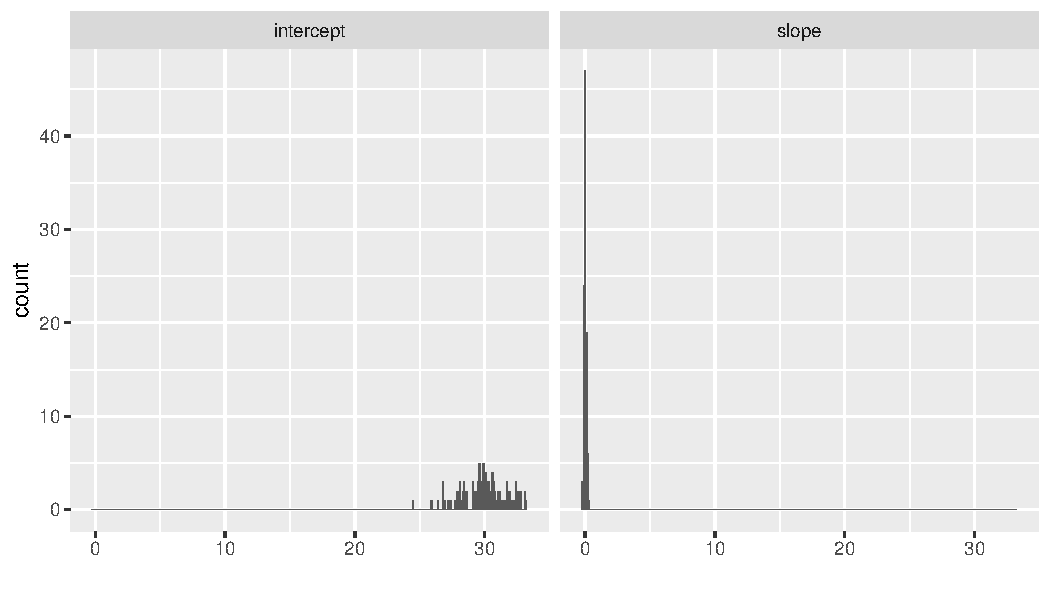
\includegraphics[width=\maxwidth]{figure/inf_3b-1} 

}

\caption[Distribution of the 100 sample intercepts and 100 sample slope]{Distribution of the 100 sample intercepts and 100 sample slope.}\label{fig:inf_3b}
\end{figure}


\end{knitrout}




\begin{knitrout}
\definecolor{shadecolor}{rgb}{0.969, 0.969, 0.969}\color{fgcolor}\begin{figure}

{\centering 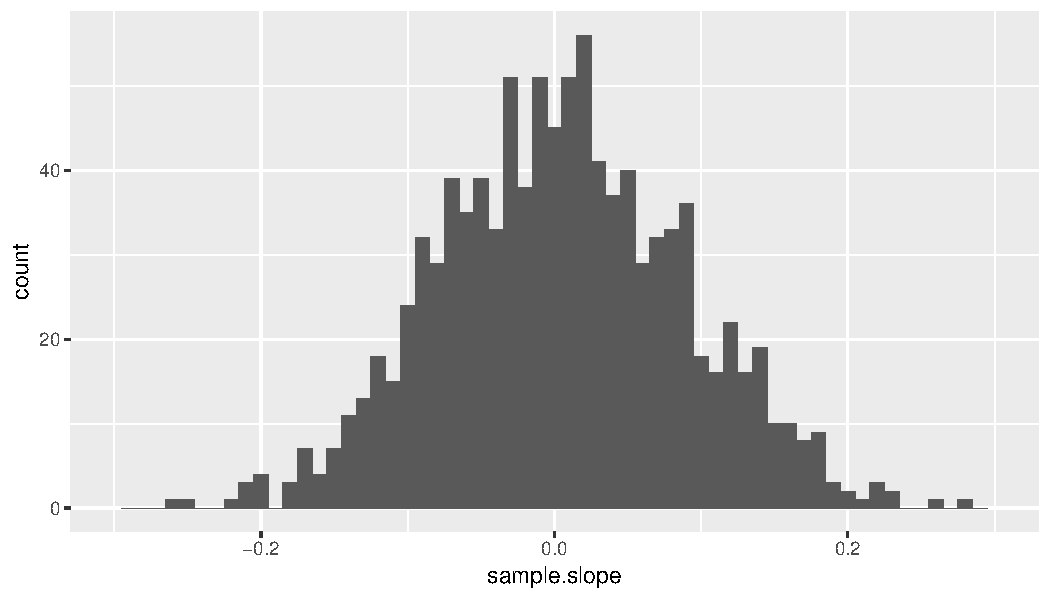
\includegraphics[width=\maxwidth]{figure/inf_5-1} 

}

\caption[Distribution of 1000 sample slopes]{Distribution of 1000 sample slopes.}\label{fig:inf_5}
\end{figure}


\end{knitrout}

For now, let's focus on the slope; this because we are mostly interested in the linear relationship between volume and temperature. However, everything that follows also applies to the intercept. In Figure \ref{fig:inf_5} we see the histogram of the slopes if we carry out the random sampling 1000 times. We see that on average the sample slope is around $0.001$, which is the population slope (the slope if we analyze all bottles). But there is variation around that mean of $0.001$: the standard deviation of all 1000 sample slopes turns out to be 0.084.


The standard deviation of the sample slopes is called the \textit{standard error}. Had the population slope been 110 or -40, the sample slopes would cluster around 110 or -40, but the standard deviation of the sample slopes, the standard error, would be the same.

The standard error for a sample slope represents the uncertainty about the population slope. If the standard error is large, it means that if we would draw many different random samples from the same population data, we would get very different sample slopes. If the standard error is small, it means that if we would draw many different random samples from the same population data, we would get sample slopes that are very close to one another, and very close to the population slope.\footnote{Because sample slopes cluster around the population slope, the sample slope is very close to the population slope when the standard error is small.}


\subsection{Standard error and sample size}\label{sec:sampsizese}

The standard error for a sample slope depends on many things, but the most important factor is the \textit{sample size}: how many bottles there are in each random sample. The larger the sample size, the smaller the standard error, the more certain we are about the population slope. In the above example, the sample size is 200 bottles.

% In the above bottle example, the standard deviation of all 80,000 volumes was sd(bottles$volume), where most of the volumes (roughly 95\%) lie between 28 and 32 cl. The variance is the square of the standard deviation so the variance is var(bottles$volume). Now imagine that we have another population, say bottles from a different brand, where we see a much smaller variation in volumes: suppose the average volume is also 30, but the standard deviation is 0.5, so that roughly 95\% of the scores lie between 29 and 31. If we then take 1000 samples from this distribution of bottles from this other brand, we get the distribution in Figure \ref{fig:inf_6}.

% <<inf_6 ,fig.height=4, echo=FALSE, fig.align='center', fig.cap='Distribution of the sample mean when population variance is 25 and sample size equals 200.'>>=
% set.seed(1234)
% bottles <- data.frame(ID=1:800000,
%                       volume= round(rnorm(800000, 30, 0.5 ),2),
%                       temperature=  round(runif(800000, 18,21 ),2)                 )
% sample.intercept <- c()
% sample.slope <- c()
% for (i in 1:1000)
% {
%         sample <- bottles[sample(1:80000,200),]
%         out <- lm(volume~temperature, sample)
%         sample.intercept[i] <- out$coef[1]
%         sample.slope[i] <- out$coef[2]
% }
% data.frame(sample.slope) %>% ggplot(aes(x=sample.slope)) +geom_histogram(binwidth = 0.01) +  xlim(c(-0.3,0.3))
% @

% Now we see that the sample slopes cluster much closer around the value of 0. The standard deviation of this distribution, that is, the standard error, is now much smaller: sd(sample.slope). This makes sense: the larger the variation at population level, the higher the probability that you find extreme values in your sample that influence the sample slope upwards or downwards. The smaller the variation at population level, the higher the proportion of data points in your sample that are very close to the population slope, so that the sample intercept will be very close to the population slope In sum: the higher the population variance, the larger the standard error, the larger the uncertainty about the population slope.

Imagine that you draw only 2 bottles from the population of 80,000 bottles. Then there is quite some probability that by sheer luck you find one bottle with a low temperature and a small volume, and another bottle with a high temperature and a large volume. This would yield a sample slope that is quite large and positive. But there is an equally high probability that you get one bottle with a low temperature with a large volume, and another bottle with a high temperature and a small volume. Then based on these two other bottles, the sample slope will be large and negative. In case of a sample size of only 2, you see that there will be quite a lot of variation in the sample slope if we draw various random samples. This large variation in sample slopes is then captured by the standard error, that will be large. With only 2 bottles per sample, the uncertainty about the population slope will then also be large. The left panel of Figure \ref{fig:inf_7} shows the distribution of the sample slope where the sample size is 2. You see that for quite a number of samples, the slope is larger than 10, even if the population slope is 0.001.

Now imagine that your sample size is 20. Then the probability that the 20 bottles will result in a large variation of slopes will be smaller: it would be very unlikely that \textit{all} 20 bottles have either a high volume and a high temperature, or a low volume and a low temperature. If there happen to be a few of such bottles in the sample, the other bottles will average these effects out. Take a look at Table \ref{tab:samplesize20}. There we see measurements on a random sample of 20 bottles. The first bottle shows a relatively low volume and a relatively low temperature measure. The second bottle shows the opposite: a relatively large volume and a relatively high temperature. This is also depicted in Figure \ref{fig:fig_samplesize20}. Had our sample size been only 2, then on the basis of these two bottles we would have found a highly positive slope coefficient (a high correlation). However, since our sample size is 20, there are many other bottles in our sample, including bottles that have relatively high volumes but relatively low temperatures measures, and vice versa: bottles with relatively low volumes and relatively high volumes, see Figure \ref{fig:fig_samplesize20}. Combined with all the other bottles, we would not find a very strong positive slope coefficient, because in the population of 80,000 bottles there is no such strong slope. The fact that we found one with the two bottles was just sheer coincidence. With large numbers of observations, you are less prone to chance observations. With large sample sizes, your results from a regression analysis become less dependent on chance, become more stable, and therefore more reliable. 

% latex table generated in R 3.5.0 by xtable 1.8-2 package
% Mon Jan 21 16:42:28 2019
\begin{table}[ht]
\centering
\caption{A random sample of 20 bottles with their beer volumes and their logged temperature.} 
\label{tab:samplesize20}
\begin{tabular}{rrr}
  \hline
bottle & volume & temperature \\ 
  \hline
 1 & 28.0 & 18 \\ 
   2 & 32.0 & 21 \\ 
   3 & 29.2 & 20 \\ 
   4 & 30.3 & 21 \\ 
   5 & 30.2 & 20 \\ 
   6 & 31.3 & 19 \\ 
   7 & 28.9 & 19 \\ 
   8 & 28.6 & 20 \\ 
   9 & 30.0 & 19 \\ 
  10 & 28.5 & 20 \\ 
  11 & 30.4 & 21 \\ 
  12 & 31.7 & 19 \\ 
  13 & 31.5 & 20 \\ 
  14 & 30.4 & 19 \\ 
  15 & 27.9 & 20 \\ 
  16 & 29.5 & 18 \\ 
  17 & 29.9 & 19 \\ 
  18 & 30.7 & 19 \\ 
  19 & 30.9 & 18 \\ 
  20 & 28.8 & 18 \\ 
   \hline
\end{tabular}
\end{table}


\begin{figure}

{\centering 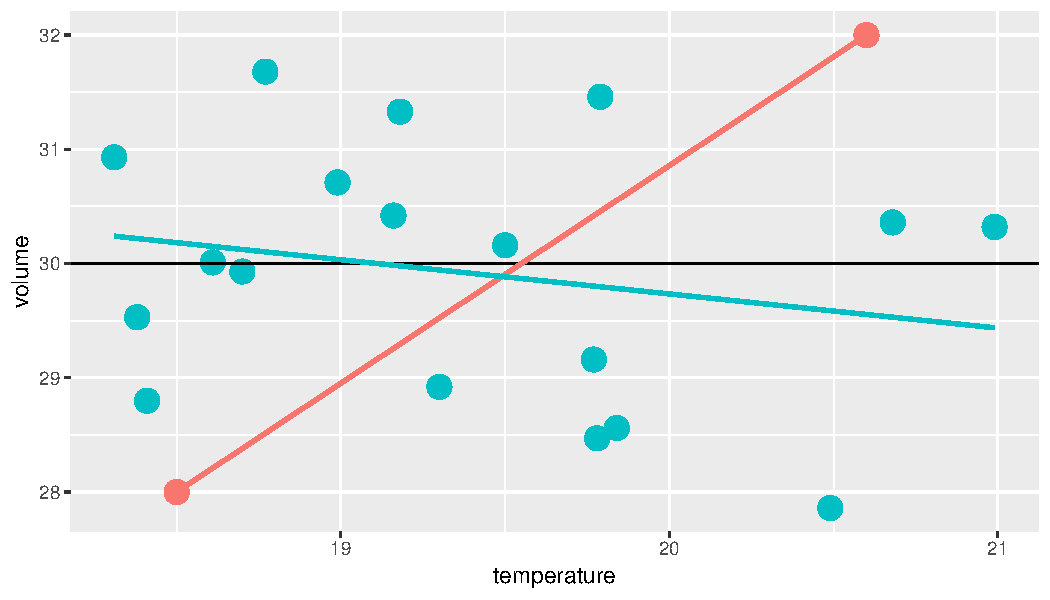
\includegraphics[width=\maxwidth]{figure/fig_samplesize20-1} 

}

\caption[The averaging effect of increasing sample size]{The averaging effect of increasing sample size. The figure shows the relationship between temperature and volume for a random sample of 20 bottles; the first two bottles are marked in red. The red line would be the sample slope based on the first two bottles, the blue line is the sample slope based on all 20 bottles, and the black line represents the population slope, based on all 80,000 bottles.}\label{fig:fig_samplesize20}
\end{figure}




Because of this averaging effect, the slope based on 20 bottles will then be closer to the population slope. The standard error therefore decreases with increasing sample size. With a sample size of 20, most slopes are between -0.6 and 0.6.

In Figure \ref{fig:inf_7} we see the distributions of the sample slope where the sample size is either 2 (left panel) or 20 (right panel). We see quite a lot of variation in sample slopes with sample size equal to 2, and considerably less variation in sample slopes if sample size is 20. This shows that the larger the sample size, the smaller the standard error, the larger the certainty about the population slope. 




\begin{knitrout}
\definecolor{shadecolor}{rgb}{0.969, 0.969, 0.969}\color{fgcolor}\begin{figure}

{\centering 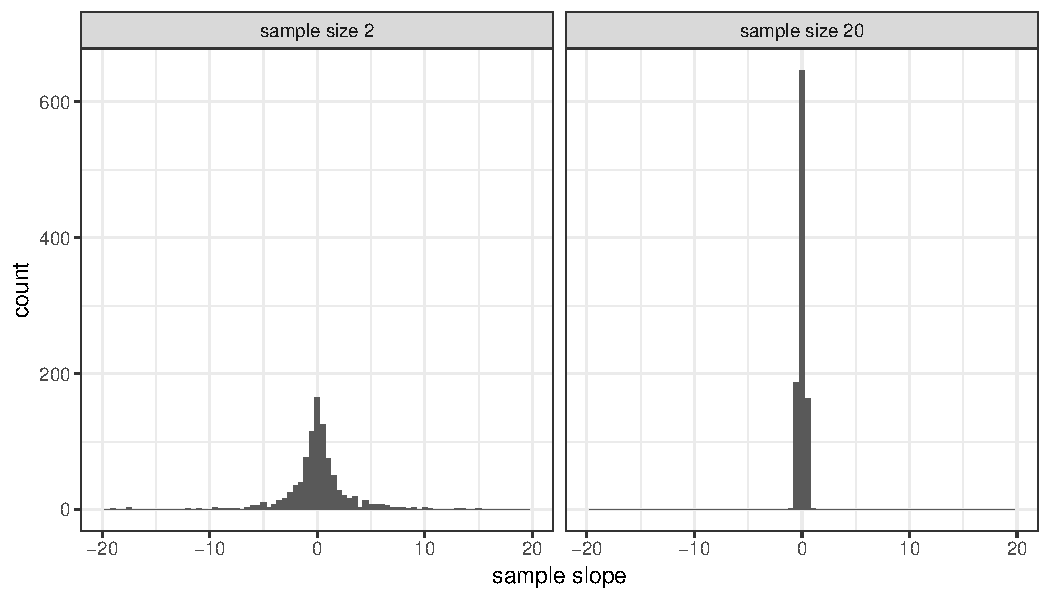
\includegraphics[width=\maxwidth]{figure/inf_7-1} 

}

\caption[Distribution of the sample slope when sample size is 2 (left panel) and when sample size is 20 (right panel)]{Distribution of the sample slope when sample size is 2 (left panel) and when sample size is 20 (right panel).}\label{fig:inf_7}
\end{figure}


\end{knitrout}


\subsection{From sample slope to population slope}

In the previous section we saw that if we have a small standard error, we can be relatively certain that our sample slope is close to the population slope. We did a thought experiment where we knew everything about the population intercept and slope, and we drew many samples from this population. In reality, we don't know anything about the population: we only have one sample of data. So suppose we draw a sample of 200 from an unknown population of bottles, and we find a slope of 1, we have to look at the standard error to know how close that sample slope is to the population slope.

For example, suppose we find a sample slope of 1 and the standard error is equal to 0.1. Then we know that the population slope is more likely to be in the neighbourhood of values like 0.9, 1.0, or 1.1 than in the neighbourhood of 10 or -10.

Now suppose we find a sample slope of 1 and the standard error is equal to 10. Then we know that the sample slope is more likely to be somewhere in the neighbourhood of values like -9, 1 or 11, than around values in the neighbourhood of -100 or +100. However, values like -9, 1 and 11 are quite far apart, so actually we have no idea what the population slope is; we don't even know whether the population slope is positive or negative! The standard error is simply too large.

As we have seen, the standard error depends very much on sample size. Apart from sample size, the standard error for a slope also depends on the variance of the independent variable, the variance of the dependent variable, and the correlations between the independent variable and other independent variables in the equation (in case of multiple regression and other linear models, see later chapters). We will not bore you with the complicated formula for the standard error for regression coefficients \footnote{See https://www3.nd.edu/~rwilliam/stats1/x91.pdf for the formula. In this pdf, 'IV' means independent variable}. Instead, we look at the standard error that SPSS or other computer packages compute for us.



% % \begin{equation}
% % \sigma_{\bar{y}} = \frac{\sigma}{\sqrt{n}}
% % \end{equation}
% %
% % where $\sigma$ is the population standard deviation and $n$ is sample size. Sample size we know, this is 100, but how about the population standard deviation? We don't know anything about the population, that's the whole reason that we took a sample. But we do know the standard deviation in the sample data. It turns out the \textit{sample standard deviation} $s$ is a rough approximation of the population variance. Therefore we often see the following formula for a standard error
% %
% % \begin{equation}
% % \sigma_{\bar{y}} = \frac{s}{\sqrt{n}}
% % \end{equation}
% %
% %
% % where $s$ represents an approximation of the population standard deviation using the sample data, more specifically the sums of squares (SS, see Chapter 1).
% % \begin{equation}
% % s = \sqrt{\frac{SS}{n-1}}
% % \end{equation}
% %
% % Note the similarity between the standard deviation of a particular set of values, $\sigma=\sqrt{\frac{SS}{n}}$ and the formula for $s$: if you're interested in the standard deviation for a specific set of values, then you use $\sigma=\sqrt{\frac{SS}{n}}$, if you're interested in the standard deviation of the population that a set of numbers is a random sample of, then you use $s=\sqrt{\frac{SS}{n-1}}$.\footnote{Confusingly, $s$ is often called the $sample standard deviation$, while it is really an approximation of the population standard deviation based on the sample data.}
% %
% % Suppose in the Paris data we find an $s$ of 12, then we know that the standard error is equal to $\frac{12}{\sqrt{100}}=12/10$.



\section{$t$-distributions}

Above we saw that if there is a large collection of data points (population) with a particular slope that describes the relationship between two variables, and if you then take random samples out of this collection, each time you find a different value for the slope in the sample, the sample slope. We saw that the standard deviation of the distribution of all such slopes is called the standard error. The standard error gives us information about how certain we can be that the slope in the sample is close to the slope in the population. The smaller the standard error, the more certain we can be that the population slope has a value in the neighbourhood of the value for the sample slope.



\begin{knitrout}
\definecolor{shadecolor}{rgb}{0.969, 0.969, 0.969}\color{fgcolor}\begin{figure}

{\centering 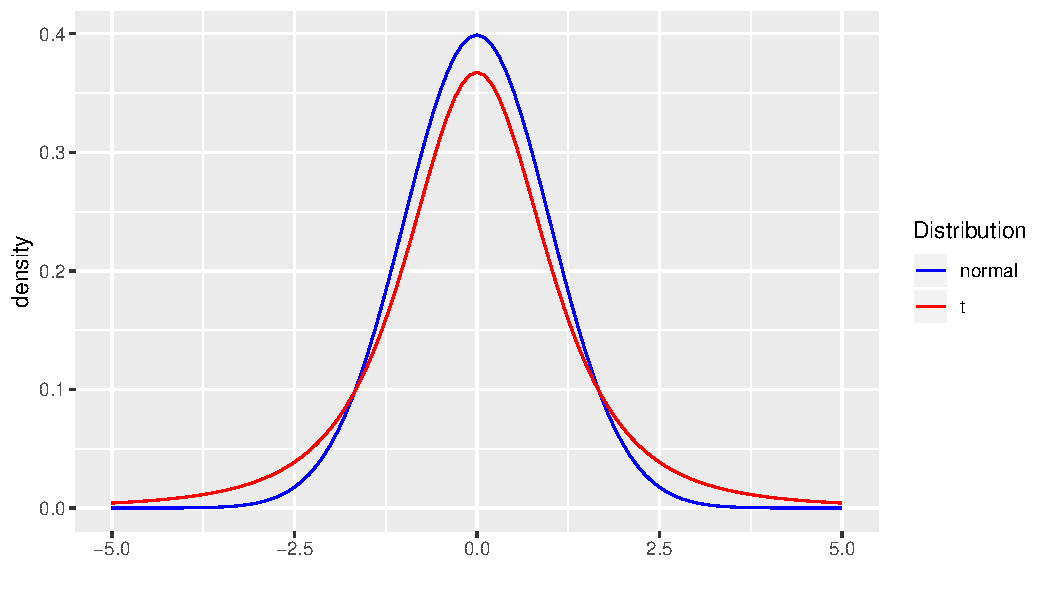
\includegraphics[width=\maxwidth]{figure/inf_8-1} 

}

\caption[Difference in the shapes of a normal distribution and a t-distribution]{Difference in the shapes of a normal distribution and a t-distribution}\label{fig:inf_8}
\end{figure}


\end{knitrout}



When we look at the distribution of the sample slope, for instance in Figure \ref{fig:inf_5}, we notice that the distribution looks very much like a normal distribution. Well, actually it isn't quite a normal distribution. In reality it has the shape of a $t$-distribution. Figure \ref{fig:inf_8} shows the difference between a $t$-distribution (in red) and a normal distribution (in blue). In this figure, the means are equal (0) and the areas under the curve are equal (1), but the shapes are clearly different. Compared to the $t$-distribution, the normal distribution has more observed values close to the mean (the distribution is more peaked). The $t$-distribution has relatively more observations in the tails of the distribution (heavy tails).



Actually, the shape of the distribution of sample slopes depends on the size of the samples, the sample size. In Figure \ref{fig:inf_9} we see what the distribution of sample slopes would look like if all samples would be of size 4 (the red line) and what the distribution would look like if sample size would be 200 (the blue line). If we compare the blue lines in Figures \ref{fig:inf_8} and \ref{fig:inf_9} we see that the shape of the $t$-distribution for a sample size of 200 looks extremely close to the normal distribution. Remember: we are talking here only about the \textit{shape} of the distribution.\footnote{The variance (i.e., the square of the standard error) will be smaller for larger samples sizes.} 


In summary, when we draw many samples from a population, the standard deviation of the sample slopes (the standard error) will be smaller for a large sample size than for a small sample size. In addition, the \textit{shape} of the distribution of sample slopes is that of a $t$-distribution. The shape of the $t$-distribution also depends on sample size. The larger the sample size, the more the shape of the $t$-distribution looks like a normal distribution. Thus, for large sample sizes, the distribution of sample slopes shows very little variance with a shape closely resembling a normal distribution.


\begin{knitrout}
\definecolor{shadecolor}{rgb}{0.969, 0.969, 0.969}\color{fgcolor}\begin{figure}

{\centering 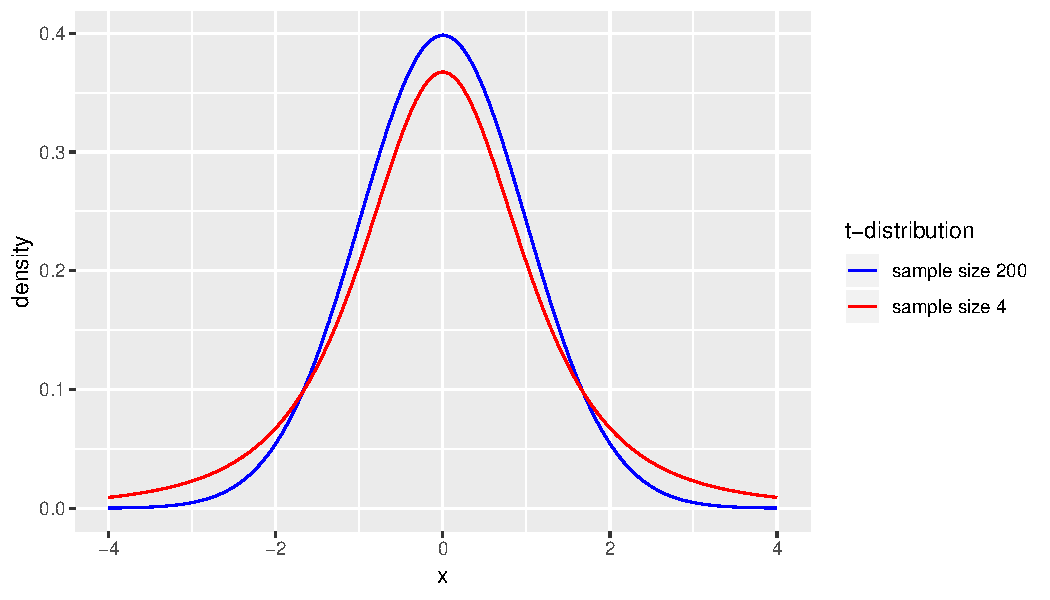
\includegraphics[width=\maxwidth]{figure/inf_9-1} 

}

\caption[The shape of the distribution of sample slopes depends on sample size]{The shape of the distribution of sample slopes depends on sample size.}\label{fig:inf_9}
\end{figure}


\end{knitrout}





\section{$T$-statistics}


Above we saw that sample slopes have a $t$-distribution, and that if sample size is large, say larger than 200, the $t$-distribution looks very much like a normal distribution. From the normal distribution, we know that if we standardize the scores by computing $Z$-scores, that is, if we subtract the mean and then divide by the standard deviation, $Z= \frac{x-\bar{x}}{\sigma}$, then 2.5\% of the $Z$-values is smaller than -1.96 and 2.5\% of the $z$-values is larger than +1.96.


Therefore, if for large sample sizes the $t$-distribution is practically indistinguishable from the normal distribution, we know that if we standardize the sample slope values, we get a similar result. Instead of looking at the actual slope value, we can compute a standardized slope. Let's call that standardized result $T$. Then we get:


\begin{equation}
T = \frac{b-\bar{b}}{se}
\end{equation}

In words: we take a particular sample slope $b$ and we subtract the mean from all sample slopes. The result we divide by the standard deviation of the sample slopes, which is callled the standard error $se$.

But what is the mean sample slope? Since the sample slopes cluster around the population slope $\beta$, the average of all possible samples slopes is equal to $\beta$. Thus we have:

\begin{equation}
T = \frac{b-\beta}{se}
\end{equation}


Let's go back to the example of the beer bottles. In our first random sample of 200 bottles, we found a sample slope of -0.088. We also happened to know the population slope, which was 0.001. From our computer experiment, we saw that the standard deviation of the sample slopes with sample size 200 was equal to 0.084. Thus, if we fill in the formula for the standardized slope $T$, we get for this particular sample


\begin{equation}
T = \frac{-0.088-0.001}{0.084}= -1.06
\end{equation}


Notice that we distinguish between a variable $t$ that has a $t$-distribution, and a $T$-statistic that is based on a computation.


Now, what can we say about this $T$-value? Since with a sample size of 200 the distribution of sample slopes closely resembles a normal distribution, we can use normal tables published online or in computer packages to see how likely a value of $T=-1.06$ actually is. In normal tables we find that a $Z$-value of $-1.06$ is not that strange: in the standard normal distribution, $14.457$\% of the values is smaller than $-1.06$. The area is shown in Figure \ref{fig:inf_9b}.


\begin{knitrout}
\definecolor{shadecolor}{rgb}{0.969, 0.969, 0.969}\color{fgcolor}\begin{figure}

{\centering \includegraphics[width=\maxwidth]{figure/inf_9b-1} 

}

\caption[The standard normal distribution and the probability of a Z-score lower than -1.06]{The standard normal distribution and the probability of a Z-score lower than -1.06}\label{fig:inf_9b}
\end{figure}


\end{knitrout}


When would we say that a certain $T$-value would cause concern? Well, perhaps we could say that if the $T$-value were 3 standard deviations away from the population value, either 3 standard deviations above the population value or 3 standard deviations below the population value. From the normal tables, we know that that happens only $0.27$\% of the time.

Alternatively, we could say that we would perhaps also be worried if the sample slope were 2 standard deviations away from the population slope, corresponding to $T$-value of 2 or -2. We know that the probabilty that that happens is around 5\%, small enough perhaps to raise concern about our knowledge about the population slope.

In this section, when discussing $T$-statistics, we assumed we knew the population slope $\beta$, that is, the slope of the linear equation based on all 80,000 bottles. In reality, we never know the population slope: the whole reason to look at the sample slope is to have an idea about the population slope. Let's look at some hypothetical population slopes.





\section{Hypothetical population slopes}


Since we don't know the actual value of the population slope $\beta$, we could ask the personnel in the beer factory what they think is a likely value for the slope. Suppose Mark says he believes that a slope of 2 could be true. Well, let's find out whether that is a reasonable guess. Now we \textit{assume} that the population slope $\beta$ is 2, and we compute the $T$-statistic for our sample slope:



\begin{equation}
T = \frac{-0.088-2}{0.084}= -24.8
\end{equation}

From the normal distribution, we know that such a $T$-value is very unlikely: the probability of finding a sample slope -24.8 standard deviations away form a population slope of 2 is less than 0.00000000000000000000000000000000001. Because we know that such a $T$-value of -24.8 is unlikely, we know that a sample slope of -0.0879535 is unlikely \textit{if the population slope is equal to 2}. Therefore, we feel 2 is not a realistic value for the population slope.


Now let's ask Martha. She thinks a reasonable value for the population slope is 0, as she doesn't believe there is a linear relationship between temperature and volume. She feels that the fact that we found a sample slope that was not 0 was a pure coincidence. Based on that hypothesis, we compute $T$ again and find:


\begin{equation}
T = \frac{-0.088-0}{0.084}= -1.046
\end{equation}

In other words, if we believe Martha, our sample slope is only about 1 standard deviation away from her hypothesized value. That's not a very bad idea, since from the normal distribution we know that the probability of finding a value more than 1.05 standard deviations away from the mean (above or below) is $29.54$\% (you can see that more or less from Figure \ref{fig:inf_9b}). In other words, if the population slope is truly 0, then our sample slope of $-0.088$ is quite a reasonable finding. If we reverse this line of reasoning: if our sample slope is $-0.088$, with a standard error of $0.084$, then a population slope of 0 is quite a reasonable guess! It is reasonable, since the difference between the sample slope and the hypothesised value is only $-1.046$ standard errors.

So when do we no longer feel that a person's guess of the population slope is reasonable? Perhaps if the probability of finding a sample slope of at least a certain size given a hypothesised population slope is so small that we no longer believe that the hypothesised value is reasonable. We might for example choose a small probability like 1\%. We know from the normal distribution that 1\% of the values lie at least $2.58$ standard deviations above and below the mean. This is shown in Figure \ref{fig:normal_2z}. So if our sample slope is more than $2.58$ standard errors away from the hypothesised population slope, then that population slope is \textit{not} a reasonable guess. In other words, if the \textit{distance} between the sample slope and the hypothesised population slope is more than 2.58 standard errors, then the hypothesised population slope is no longer reasonable.

\begin{knitrout}
\definecolor{shadecolor}{rgb}{0.969, 0.969, 0.969}\color{fgcolor}\begin{figure}

{\centering \includegraphics[width=\maxwidth]{figure/normal_2z-1} 

}

\caption[The standard normal distribution]{The standard normal distribution.}\label{fig:normal_2z}
\end{figure}


\end{knitrout}

\begin{knitrout}
\definecolor{shadecolor}{rgb}{0.969, 0.969, 0.969}\color{fgcolor}\begin{figure}

{\centering \includegraphics[width=\maxwidth]{figure/normal_2z2-1} 

}

\caption[The standard normal distribution]{The standard normal distribution.}\label{fig:normal_2z2}
\end{figure}


\end{knitrout}

This implies that \textit{any} value closer than $2.58$ standard errors from the sample slope is a collection of reasonable values for the population slope.

Thus, in our example of the 200 bottles with a sample slope of $-0.088$ and a standard error of $0.084$, the interval from $-0.088- 2.58 \times 0.084$ to $-0.088+ 2.58 \times 0.084$ contains reasonable values for the population slope. If we do the calculation, we get the interval from $-0.3$ to $0.13$. This is plotted in Figure \ref{fig:normal_2z2}. If we would have to guess the value for the population slope, our guess would be that it would lie somewhere between between -0.30 and $0.13$, \textit{if we feel that 1\% is a small enough probability}.

In data analysis, such an interval that contains reasonable values for the population value, if we only know the sample value, is called a \textit{confidence interval}. Here we've chosen to use $2.58$ standard errrors as our cut-off point, because we felt that 1\% would be a small enough probability to dismiss the real population value as a reasonable candidate. Such a confidence interval based on this 1\% cut-off point is called a 99\% confidence interval.

One often also sees 95\% confidence intervals, particularly in social and behavioural sciences. Because with the normal distribution, 5\% of the observations lie more than 1.96 standard deviations away from the mean, the 95\% confidence interval is constructed by subtracting/addding 1.96 standard errors from/to the sample value. Thus, in the case of our bottle sample, the 95\% confidence interval for the population slope is from $-0.088- 1.96* 0.084$ to $-0.088+ 1.96* 0.084$, so reasonable values for the population slope are those values between $-0.25$ and $0.08$. Luckily, this corresponds to the truth, because we happen to know that the population slope is equal to 0.001. In real life, we don't know the population slope and of course it might happen that the true population value is not within the 95\% confidence interval. If you want to make the probability of this being the case smaller, then you can use a 99\%, a 99.9\% or an even larger confidence interval.


\section{Confidence intervals for smaller sample sizes}

In the previous section we used the normal distribution to come up with 95\% and 99\% confidence intervals for the slope coefficient. These were constructed using 1.96 and $2.58$ times the standard error, respectively. However, these numbers 1.96 and $2.58$ can only be used when the sample size is large enough to say that the distribution of the sample slope is very close to a normal distribution. Earlier, we saw that the distribution of the sample slope is actually a $t$-distribution, that doesn't look normal at all for small sample sizes. Therefore, for small sample sizes, we need to know the cut-off points that correspond to 5\% and 1\% probabilities for the $t$-distribution.








% In data analysis, one often uses a \textit{confidence interval} to indicate a range of reasonable values for the population value. Here we found a sample slope of 112. Now imagine that 112 were also the population slope. Then if we would draw many random samples of size 100, we know from the computed standard error of 12/10 that roughly 95\% of the sample means would lie between $112 - 2 \times 12/10 = 109.6$ and $112 + 2 \times 12/10 = 114.4$.

% Now suppose that the true population mean were not 112 but 114.4. In that case, if we draw many samples of size 100, we could reasonably find a value of 112, since 95\% of the sample mean would then lie between $114.4 - 2 \times 12/10 = 112$ and $114.4 + 2 \times 12/10 = 116.8$. So even if the true population mean were 112.4, it's very possible that we could find a sample slope of ?. We cannot neglect the possiblity that the true slope is 114.4. Similarly, we cannot neglect the possibility that the true slope is 109.6, because if the true mean were 109.6, 95\% of the sample means of size 100 would lie between $109.6 - 2 \times 12/10 = 107.2$ and $109.6 + 2 \times 12/10 = 112$. So our range of reasonable values for the population slope would be somewhere between 107.2 and 114.4. This range is referred to as the \textit{95\% confidence interval}. The 95\% confidence interval can be computed by subtracting and adding twice the standard error of the mean to the sample mean.


% For large sample sizes we can approximate the $t$-distribution by a normal distribution so that we know that 95\% of the observations lie between -1.96 and +1.96 times the standard deviation. For small sample sizes we have to use a $t$-distribution to construct confidence intervals. For small sample sizes, we need to know the particular shape of the distribution to find out where the middle 95\% of the sample means lie.

\begin{knitrout}
\definecolor{shadecolor}{rgb}{0.969, 0.969, 0.969}\color{fgcolor}\begin{figure}

{\centering \includegraphics[width=\maxwidth]{figure/inf_10-1} 

}

\caption[Two t-distributions when sample size is 4 or 200, with corresponding 95 percent intervals]{Two t-distributions when sample size is 4 or 200, with corresponding 95 percent intervals.}\label{fig:inf_10}
\end{figure}


\end{knitrout}



Figure \ref{fig:inf_10} shows the case for the situation where the population slope is 0 and the sample size is 4. Suppose the standard error is equal to 1. Then this figure shows that roughly 95\% of the sample slopes lie between $\pm$ 4.30 standard errors below and above the mean (the red lines). In the same figure we also see that if sample size is 200, 95\% of the sample means lie between $\pm$ 1.97 standard errors below and above the mean (the blue line). This is almost the same as for the normal distribution, where 95\% of the observations lie between $\pm$ 1.96 standard deviations below and above the mean.

Because for every sample size, the middle region where 95\% of the observations lie is different, there are tables available where these values can be found. However, these tables are built-in in every statistical package, so it is far easier to let SPSS construct the 95\% confidence intervals for us.


% latex table generated in R 3.5.0 by xtable 1.8-2 package
% Mon Jan 21 16:42:32 2019
\begin{table}[ht]
\centering
\caption{Quantiles for the standard normal and several t-distributions.} 
\label{tab:table_1}
\begin{tabular}{rrrrrrr}
  \hline
probs & norm & t198 & t100 & t50 & t10 & t2 \\ 
  \hline
0.0005 & -3.29 & -3.34 & -3.39 & -3.50 & -4.59 & -31.60 \\ 
  0.0010 & -3.09 & -3.13 & -3.17 & -3.26 & -4.14 & -22.33 \\ 
  0.0050 & -2.58 & -2.60 & -2.63 & -2.68 & -3.17 & -9.92 \\ 
  0.0100 & -2.33 & -2.35 & -2.36 & -2.40 & -2.76 & -6.96 \\ 
  0.0250 & -1.96 & -1.97 & -1.98 & -2.01 & -2.23 & -4.30 \\ 
  0.0500 & -1.64 & -1.65 & -1.66 & -1.68 & -1.81 & -2.92 \\ 
  0.1000 & -1.28 & -1.29 & -1.29 & -1.30 & -1.37 & -1.89 \\ 
  0.9000 & 1.28 & 1.29 & 1.29 & 1.30 & 1.37 & 1.89 \\ 
  0.9500 & 1.64 & 1.65 & 1.66 & 1.68 & 1.81 & 2.92 \\ 
  0.9750 & 1.96 & 1.97 & 1.98 & 2.01 & 2.23 & 4.30 \\ 
  0.9900 & 2.33 & 2.35 & 2.36 & 2.40 & 2.76 & 6.96 \\ 
  0.9950 & 2.58 & 2.60 & 2.63 & 2.68 & 3.17 & 9.92 \\ 
  0.9990 & 3.09 & 3.13 & 3.17 & 3.26 & 4.14 & 22.33 \\ 
  0.9995 & 3.29 & 3.34 & 3.39 & 3.50 & 4.59 & 31.60 \\ 
   \hline
\end{tabular}
\end{table}

But let us look at a few regularities. For several probabilities, the corresponding quantiles are presented in Table \ref{tab:table_1} for the standard normal distribution and several $t$-distributions.

The shape of the $t$-distribution is indicated by its \textit{degrees of freedom}. The shape of the distribution of sample slopes when sample size is 200, is a $t$-distribution with 198 degrees of freedom. The shape of the distribution of sample slopes when sample size is 4, is a $t$-distribution with 2 degrees of freedom. In general, the shape of the distribution of sample slopes for sample size $n$, is a $t$-distribution with $n-2$ degrees of freedom. The higher the degrees of freedom, the more the corresponding $t$-distribution looks like a normal distribution. We will come back to degrees of freedom and the $n-2$ rule in the next section.

Table \ref{tab:table_1} shows for instance the cut-off points for 2.5\% and 97.5\% for the standard normal distribution (the 0.025 and 0.975 quantiles, respectively) and the $t$-distribution with 198 degrees of freedom: 1.96 and 1.97 standard deviations (standard errors) respectively. For the $t$-distribution with 100 degrees of freedom, the cut-off point is 1.98 standard errors. This would be the appropriate $t$-distribution for a sample size of 102. But for smaller sample sizes, the increase in number of standard errors goes up quickly: with 50 degrees of freedom (sample size 52), the cutoff is 2.01, for 10 degrees of freedom it is 2.23 and for 2 degrees of freedom it becomes even 4.30 standard errors. Thus, if we have a sample size of 4, we construct a 95\% confidence interval of 4.30 standard errors below the sample slope and 4.30 standard errors above the sample slope.

If you want to have the 99\% confidence interval, you look at the cut-off points for 0.005 and 0.995 which are -2.58 and +2.58, respectively, for the normal distribution, but -9.92 and +9.92 for a $t$-distribution with 2 degrees of freedom. Suppose we sample 4 bottles and find a sample slope of 5 with a standard error of 4, then the 99\% confidence for the slope is from $5-9.92\times 4$ to $5+9.92\times 4$, so from -34.68 to 44.68, which is of course a huge interval. On the other hand, a sample of only 4 bottles is of course very small. It makes intuitive sense that if you have only 4 bottles to go on, you are very uncertain about the population slope: it could be anything!

In short, we can look up the cut-off points for 95\%, 99\% and other intervals from tables online, in books, or in statistical packages. Generally, the smaller the sample size, the lower the degrees of freedom, the larger the number of standard errors you need to construct your confidence intervals.






\subsection{Exercises}

\begin{enumerate}


\item Suppose we randomly pick 102 students from the University of Twente and determine the linear equation between age in years (independent variable) and height in cms (dependent variable). Suppose we find a slope coefficient of 0.010, with a standard error of 0.009. 

\subitem Construct the 95\% confidence interval for the slope in the entire population in UT students using table \ref{tab:nonparmixed_4}.

\subitem What can we say about values within this constructed confidence interval?

\subitem Suppose a professor believes the true slope is equal to 0: is that a reasonable belief given the finding of a sample slope of 0.010? Motivate your answer using the 95\% confidence interval.


\item Suppose we randomly pick 52 adult inhabitants of Tuvalu and determine the linear equation between age in years (independent variable) and height in cms (dependent variable). 

\subitem Suppose we find an intercept of 168, with a standard error of 0.07. Construct the 99\% confidence interval for the intercept in the entire population of adult inhabitants of Tuvalu using Table \ref{tab:table_1}.

\subitem What can we say about values within this constructed confidence interval?

\subitem Suppose a Swedish diplomat stationed in Tuvalu believes the population intercept is equal to 169 cm: is that a reasonable belief given the finding of a sample intercept of 168? Motivate your answer using the 99\% confidence interval.




\end{enumerate}


Answers:

\begin{enumerate}

\item Sample size is 102, so degrees of freedom for the sample slope is 100. For a 95\% interval, 2.5\% of the observations should be on the left, and 2.5\% of the observations should be on the right. The cut-off quantiles should therefore be 0.025 and 0.975. These cut-off values for the $t$-distribution with 100 degrees of freedom are -1.98 and 1.98. Therefore the 95\% interval ranges from $0.010 - 1.98 \times 0.009$ to $0.010 + 1.98 \times 0.009$, so from -0.008 to 0.028.

\subitem These values are all reasonable values for the slope in the population of University of Twente students.

\subitem Yes, the value of 0 lies within the range from -0.008 to 0.028, so 0 is a reasonable value for the population slope.

\item Sample size is 52, so degrees of freedom for the sample slope is 50. For a 99\% interval, 0.5\% of the observations should be on the left, and 0.5\% of the observations should be on the right. The cut-off quantiles should therefore be 0.005 and 0.995. The 99\% cut-off values for the $t$-distribution with 100 degrees of freedom are therefore -2.68 and 2.68. Thus, the 99\% interval ranges from $168 - 2.68 \times 0.07$ to $168 + 2.68 \times 0.07$, so from 167.8124 to 168.1876.

\subitem These values are all reasonable values for the slope in the population of all adult inhabitants of Tuvalu.

\subitem No, the value of 169 does not lie within the range from 167.8124 to 168.1876, so 169 is not a reasonable value for the population intercept.


\end{enumerate}


\section{Degrees of freedom}


What does the term, "degrees of freedom" mean? It refers to the number of independent pieces of information in a sample of data.

Suppose that we have a sample with four values: {4, 2, 6, 8}. There are four separate pieces of information here. There is no particular connection between these values. They are free to take any values, in principle. We could say that there are “four degrees of freedom” associated with this sample of data.

Now, suppose that I tell you that three of the values in the sample are 4, 2, and 6; and I also tell you that the sample average is 5. You can immediately deduce that the fourth value has to be 8. For any other value, the average would not be 5. 

Once I tell you that the sample average is 5, I am effectively introducing a \textit{constraint}. The value of the unknown fourth sample value is implicitly being determined from the other three values plus the constraint. That is, once the constraint is introduced, there are only three logically independent pieces of information in the sample. That is to say, there are only three "degrees of freedom", once the sample average is revealed.

Let's carry this example to regression analysis. Suppose I have four observations of variables $x$ and $y$, where the values for $x$ are 1, 2, 3 and 4. Each value of $y$ is one piece of information. These $y$-values could be anything, so we say that we have 4 degrees of freedom. Now suppose I use a linear equation for these data points, and suppose I only use an intercept. Let the intercept be 5 so that we have $y=5+e$. Now the first bit of information for $x=1$, $y$ could be anything, say 2. The second and third bits of information for $x=2$ and $x=4$ could also be anything, say 6 and 2. Figure \ref{fig:inf_11} shows these bits of information as dots in a scatterplot. Since we know that the intercept is equal to 5, with no slope (slope=0), we can also draw the regression line.

\begin{knitrout}
\definecolor{shadecolor}{rgb}{0.969, 0.969, 0.969}\color{fgcolor}\begin{figure}

{\centering \includegraphics[width=\maxwidth]{figure/inf_11-1} 

}

\caption[Distribution of the sample mean when sample size is 4 or 200]{Distribution of the sample mean when sample size is 4 or 200}\label{fig:inf_11}
\end{figure}


\end{knitrout}

Before we continue, you must know that if we talk about degrees of freedom in regression analysis, we generally talk about \textit{residual degrees of freedom}. We therefore look at residuals. If we compute the residuals, we have residuals -3, 1 and -3 for these data points. When we sum them we get -5. Since we know that all residuals should sum to 0 in a regression analysis (see previous chapter), we can derive the fourth residual to be +5, since only then the residuals sum to 0. Therefore, the $y$-value for the fourth data point (for $x=3$) has to be 10, since then the residual is equal to $10-5=5$.

In short, when we do a regression analysis with only an intercept, the degrees of freedom is equal to the number of data points (combinations of $x$ and $y$) minus 1, or in short notation: $n-1$, where $n$ stans for sample size.

Now let's look at the situation where we do a regression analysis with both an intercept and a slope: suppose the intercept is equal to 3 and the slope is equal to 1: $y=3+1 x+e$. Then suppose we have the same $x$-values as the example above: 1, 2 and 4. When we give these $x$-values corresponding $y$-values, 2, 6, and 3, we get the plot in Figure \ref{fig:inf_12}.

\begin{knitrout}
\definecolor{shadecolor}{rgb}{0.969, 0.969, 0.969}\color{fgcolor}\begin{figure}

{\centering \includegraphics[width=\maxwidth]{figure/inf_12-1} 

}

\caption[Distribution of the sample mean when sample size is 4 or 200]{Distribution of the sample mean when sample size is 4 or 200}\label{fig:inf_12}
\end{figure}


\end{knitrout}

The black line is the regression line that should be appropriate for these data set of four points. The blue line is the regression line based on only the three visible data points. Now the question is, is it possible for a fourth data point with $x=3$, to think of a $y$-value such that the regression line based on these four data points is equal to $y=3+1x$? In other words, can we choose a $y$-value such that the blue line exactly overlaps with the black line?

Figure \ref{fig:inf_13} shows a number of possibilities for the value of $y$ if $x=3$. It can be seen, that it is impossible to pick a value for $y$ such that we get a regression equation $y=3+1x$. The blue line for instance comes closest to the black line. This is the regression line when $y=11$. However, it does not exactly overlap the black line. If you lower values for $y$ such as 9.5 (green line) or 8 (red line), the regression lines still not overlap, nor for a higher value of $y$ such as 12 (purple line).

\begin{knitrout}
\definecolor{shadecolor}{rgb}{0.969, 0.969, 0.969}\color{fgcolor}\begin{figure}

{\centering \includegraphics[width=\maxwidth]{figure/inf_13-1} 

}

\caption[Different regression lines for different values of y if x=3]{Different regression lines for different values of y if x=3.}\label{fig:inf_13}
\end{figure}


\end{knitrout}

So, with 4 data points, we can never freely choose 3 residuals in order to satisfy the constraint that a particular regression equation holds. We have less then 3 degrees of freedom because it is impossible to think of a fitting fourth value. It turns out, that in this case we can only choose 2 residuals freely, and the remaining residuals are then already determined. To prove this requires matrix algebra, but the gist of it is that if you have a regression equation with both an intercept and a slope, the degrees of freedom is equal to the number of data points (sample size) minus 2: $n-2$.

Generally, these degrees of freedom based on the number of residuals that could be freely chosen, given the constraints of the model, are termed \textit{residual degrees of freedom}. When using regression models, one usually only reports these residual degrees of freedom. Later on in this book, we will see instances where one also should use \textit{model degrees of freedom}. For now, it suffices to know what is meant by residual degrees of freedom.




\chapter{Inference II: hypothesis testing, $p$-values and beyond}\label{chap:hypothesis}

\section{The null-hypothesis}

Often, data analysis is about finding an answer to the question whether there is a relationship between two variables. In most cases, the question pertains to the population: is there a relationship between variable $y$ and variable $x$ in the population? In many cases, one looks for a linear relationship between two variables.

One common method to answer this question is to analyse a sample of data, apply a linear model, and look at the slope. However, one then knows the slope in the sample, but not the slope in the population. We have seen that the slope in the sample can be very different from the slope in the population. Suppose we find a slope of 1: does that mean there is a slope in the population or that there is no slope in the population?

In inferential data analysis, one often works with two hypotheses: the \textit{null-hypothesis} and the \textit{alternative hypothesis}. The null-hypothesis states that the population slope is equal to 0 and the alternative hypothesis states that there is a slope that is different from 0. Remember that if the population slope is equal to 0, that is saying that there is no linear relationship between $x$ and $y$ (that is, you cannot predict one variable on the basis of the other variable). Therefore, the null-hypothesis states there is no linear relationship between $x$ and $y$ in the population. If there is a slope, whether positive or negative, is the same as saying there is a linear relationship, so the alternative hypothesis states that there is a linear relationship between $x$ and $y$ in the population.

The null-hypothesis is often denoted as $H_0$ and the alternative hypothesis is often denoted as $H_A$. In formula form, we have


\begin{eqnarray}
H_0: \beta_{slope}=0 \\
H_A: \beta_{slope} \neq 0
\end{eqnarray}

The population slope, $\beta_{slope}$, is either 0 or it is not. Our data analysis is then aimed at determining which of these two hypotheses is true. Key is that we do a thought experiment on the null-hypothesis: we wonder what would happen if the population slope would be really 0. In our imagination we draw many samples of a certain size, say 40 data points, and then determine the slope for each sample. Earlier we learned that the many sample slopes would form a histogram in the shape of a $t$-distribution with $n-2=38$ degrees of freedom. For example, suppose we would draw 1000 samples of size 40, then the histogram of the 1000 slopes would be like depicted in Figure \ref{fig:inf_14}

\begin{knitrout}
\definecolor{shadecolor}{rgb}{0.969, 0.969, 0.969}\color{fgcolor}\begin{figure}

{\centering \includegraphics[width=\maxwidth]{figure/inf_14-1} 

}

\caption[Distribution of the sample slope when the population slope is 0 and sample size equals 40]{Distribution of the sample slope when the population slope is 0 and sample size equals 40.}\label{fig:inf_14}
\end{figure}


\end{knitrout}

From this histogram we see that all observed sample slopes are well between -0.8 and 0.8. This gives us the information we need. Of course, we have only one sample of data, and we don't know anything about the population data. But we \textit{do} know that \textit{if the population slope is equal to 0}, then it is very unlikely to find a sample slope of say 1 or -1. Thus, if we happen to find a sample slope of say -1, we know that this finding is very unlikely \textit{if we hold the null-hypothesis to be true}. In other words, if the population slope is equal to 0, it would be quite improbable to find a sample slope of -1 or smaller. Therefore, we regard the null-hypothesis to be false, since it does not provide a good explanation of why we found a sample slope of -1. In that case, we say that \textit{we reject the null-hypothesis}.

% \section{$T$-statistics}
%
% In previous sections we looked at the distribution of the slope based on sample data, if you draw many random samples from a population of data points. We saw that nearly always, the slope based on your sample data is different from the slope in the population data. We learned that the shape of the distribution is that of a $t$-distribution. The particular shape of the distribution depends on the degrees of freedom, and we learned that the degrees of freedom is equal to the number of data points in your sample (sample size $n$) minus the number of parameters/coefficients in your linear equation.
%
% We said that the distribution of the regression slope has the \textit{shape} of a $t$-distribution. In order to get a $t$-distribution, you have to standardize the scores. Similar to standardizing other scores to z-scores, by subtracting the mean and dividing by the standard deviation, we too standardize slope estimates into T-scores.
%
% Similar to the normal distribution. If you know a value is 2, then you know nothing, but if you know that a value is 20 standard deviations away from the mean, that is, a $z$-score of 20, then you know that such a value is rather unlikely.
%
% The same is true for the distribution of sample slopes. Only knowing that the sample slope is 1, says nothing, but that the slope is 30 standard errors away from a particular value is saying that such a value is unlikely.
%
% So similar to $z$-scores, we subtract the mean from the sample slope and divide by the standard deviation. If the null-hypothesis is true, the mean of the sample slopes is 0. We also know that the standard deviation of the sample slopes is the standard error.
%
% This standardized slope is called a $T$-statistic. A statistic is a quantity that is based on a calculation using your sample data. For example, using least squares, you determine the slope parameter $b_{slope}$, and you determine the standard error $se$. Next, you compute the $T$-statistic:
%
% \begin{equation}
% T = \frac{b_{slope}-0}{se} = \frac{b_{slope}}{se}
% \end{equation}
%
%
% Figure \ref{fig:inf_15} shows the $t$-distribution with $40-2=38$ degrees of freedom. This is the distribution for the $T$-statistic if our sample size is equal to 40 and the true population slope is equal to 0.
%
%
% <<inf_15,fig.height=4, echo=FALSE, fig.align='center', fig.cap='Different regression lines for different values of y if x=3.'>>=
% data.frame(x)  %>%  ggplot(aes(x=x)) +
%   stat_function(fun = dt, args = list(df=38))  +
%         ylab("density") + xlim(c(-4,4)) + xlab("T")
% @
%
% Suppose the true value of the slope (the slope in the population data) is equal to exactly 0. Then if you analyse a sample of 40 data points, you might find a slope of $b_{slope}=1$, and the standard error turns out to be 2. If we then compute $T$, we get $T=\frac{b_{slope}}{se}=1/2=0.5$. In other words, our slope is half a standard error away from the hypothesised value of 0. Whether this is a lot, depends on the shape of the distribution. For this $T$ we know that it has a $t$-distribution with 38 degrees of freedom. Figure \ref{fig:inf_16} shows this distribution. The tails that each contain 2.5\% are shaded. Thus, if the true slope is 0, and if we would draw a lot of samples and for each sample determine the slope, then 95\% of those slopes will lie within the non-shaded area. The figure also indicates the value for our T-statistic, 0.5. It can be clearly seen that a value of 0.5 lies well within the middle 95\% of the distribution, in other words, a value of 0.5 is not that strange for a $t$-distribution with 38 degrees of freedom.
%
%
% <<inf_16,fig.height=4, echo=FALSE, fig.align='center', fig.cap='Different regression lines for different values of y if x=3.'>>=
%
% df = 38; ncp = 0; limits = c(-5,5)
% lb=-20; ub=qt(0.025, df=df, ncp=ncp)
%     x <- seq(limits[1], limits[2], length.out = 100)
%     xmin <- max(lb, limits[1])
%     xmax <- min(ub, limits[2])
%     areax <- seq(xmin, xmax, length.out = 100)
%     area <- data.frame(x = areax, ymin = 0, ymax = dt(areax, df=df, ncp=ncp))
%     (ggplot()
%      + geom_line(data.frame(x = x, y = dt(x, df=df, ncp=ncp)),
%                  mapping = aes(x = x, y = y))
%      + geom_area(data = area, mapping = aes(x = x,  y = ymax))
%      + scale_x_continuous(limits = limits, breaks=seq(-5,5,1))
%      + geom_area(data = area, mapping = aes(x = seq(qt(0.975, df=df, ncp=ncp), 5, length.out = 100),  y = dt(seq(qt(0.975, df=df, ncp=ncp), 5, length.out = 100), df=df, ncp=ncp)))
%             + geom_vline(xintercept = 0.5)  + xlab("T") )
% @
%
%
%
%
%
%
%
%
%
% Based on our reasoning in the section on confidence intervals, we can construct an interval of reasonable values for the population $T$ by taking the middle 95\% of the distribution.

\section{The $p$-value}

The $p$-value is a probability. It represents the probability of observing certain events, given that the null-hypothesis is true.

In the previous section we saw that if the population slope is 0, and we drew 1000 samples of size 40, we did not observe a sample slope of -1 or smaller. In other words, the frequency of observing a slope of -1 or smaller was 0. If we would draw more samples, we theoretically could observe a sample slope of -1, but the probability that that happens for any new sample we can estimate at less than 1 in a 1000, so less than 0.001.

This estimate of the $p$-value was based on 1000 randomly drawn samples of size 40 and then looking at the frequency of certain values in that data set. But there is a short-cut, for we know that the distribution of sample slopes has a $t$-distribution if we standardize the sample slopes. Therefore we do not have to take 1000 samples and estimate probabilities, but we can look at the $t$-distribution directly, using tables online or in statistical packages.

Figure \ref{fig:inf_117} shows the $t$-distribution that is the theoretical distribution corresponding to the histogram in Figure \ref{fig:inf_14}. If the standard error is equal to 0.19, and the hypothetical population slope is 0, then the $T$-statistic associated with a slope of -1 is equal to $\frac{-1-0}{0.19}=-5.26$. With this value, we can look up in the tables, how often such a value of -5.26 \textit{or smaller} occurs in a $t$-distribution with 38 degrees of freedom (see Chapter \ref{chap:confidence}). In the tables we find that the probability that this occurs is 0.00000294. So, the fact that the $T$-statistic has a $t$-distribution gives us the opportunity to exactly determine certain probabilities, including the $p$-value.

\begin{knitrout}
\definecolor{shadecolor}{rgb}{0.969, 0.969, 0.969}\color{fgcolor}\begin{figure}

{\centering \includegraphics[width=\maxwidth]{figure/inf_117-1} 

}

\caption[The histogram of 1000 sample slopes and its corresponding theoretical t-distribution with 38 degrees of freedom]{The histogram of 1000 sample slopes and its corresponding theoretical t-distribution with 38 degrees of freedom. The vertical line represents the T-value of -5.56.}\label{fig:inf_117}
\end{figure}


\end{knitrout}

Now let's suppose we have only one sample of 40 bottles, and we find a slope of 0.1 with a standard error of 0.19. Then this value of 0.1 is $(0.1-0)/0.19=0.53$ standard errors away from 0. Thus, the $T$-statistic is 0.53. We then look at the $t$-distribution with 38 degrees of freedom, and see that such a $T$-value of 0.53 is not very strange: it lies well within the middle 95\% of the $t$-distribution (see Figure \ref{fig:inf_117}).

Let's determine the $p$-value again for this slope of 0.1: we determine the probability that we obtain such a $T$-value of 0.53 or larger. Figure \ref{fig:inf_17} shows the area under the curve for values of $T$ that are larger than 0.53. This area under the curve can be seen as a probability. The total area under the curve of the $t$-distribution amounts to 1. If we know the area of the shaded part of the total area, we can compute the probability of finding $T$-values larger than 0.53.

\begin{knitrout}
\definecolor{shadecolor}{rgb}{0.969, 0.969, 0.969}\color{fgcolor}\begin{figure}

{\centering \includegraphics[width=\maxwidth]{figure/inf_17-1} 

}

\caption[Probability of a T-value larger than 0.53]{Probability of a T-value larger than 0.53.}\label{fig:inf_17}
\end{figure}


\end{knitrout}

In tables online, in books, or available in statistical packages, we can look up how large this area is. It turns out to be 0.3. So, if the population slope is equal to 0 and we draw an infinite number of samples of size 40 and compute the sample slopes, then 30\% of them will be larger than our sample slope of 0.1. The proportion of the shaded area is what we call a \textit{one-sided} $p$-value. We call it one-sided, because we only look at one side of the $t$-distribution: we only look at values that are larger than our $T$-value of 0.53.

We conclude that a slope value of 0.1 is not that strange to find if the population slope is 0. By the same token, it would also have been probable to find a slope of -0.1, corresponding to a $T$-value of -0.53. Since the $t$-distribution is symmetrical, the probability of finding a $T$-value of less than -0.53 is depicted in Figure \ref{fig:inf_18}, and of course this probability is also 0.3.

\begin{knitrout}
\definecolor{shadecolor}{rgb}{0.969, 0.969, 0.969}\color{fgcolor}\begin{figure}

{\centering \includegraphics[width=\maxwidth]{figure/inf_18-1} 

}

\caption[Probability of finding a T-value smaller than -0.53]{Probability of finding a T-value smaller than -0.53.}\label{fig:inf_18}
\end{figure}


\end{knitrout}

Remember that the null-hypothesis is that the population slope is 0, and the alternative hypothesis is that the population slope is \textit{not} 0. We should therefore conclude that if we find a very large positive \textit{or} negative slope, large in the sense of the number of standard errors away from 0, that the null-hypothesis is unlikely to be true. Therefore, if we find a slope of 0.1 or -0.1, then we should determine the probability of finding a $T$-value that is larger than 0.53 or smaller than -0.53. This probability is depicted in Figure \ref{fig:inf_19} and is equal to twice the one-side $p$-value, $2 \times 0.2995977=0.5991953$.

\begin{knitrout}
\definecolor{shadecolor}{rgb}{0.969, 0.969, 0.969}\color{fgcolor}\begin{figure}

{\centering \includegraphics[width=\maxwidth]{figure/inf_19-1} 

}

\caption[The vertical line represents a T-value of 0.53]{The vertical line represents a T-value of 0.53. The shaded area represents the two-sided p-value: the probability of obtaining a T-value smaller than -0.53 or larger than 0.53.}\label{fig:inf_19}
\end{figure}


\end{knitrout}

This probability is called the \textit{two-sided} $p$-value. This is the one that should always be used, since the alternative hypothesis is also two-sided: the population slope can be positive or negative. The question now is: is a sample slope of 0.1 enough evidence to reject the null-hypothesis? To determine that, we determine how many standard errors away from 0 the sample slope is and we look up in tables how often that happens. Thus in our case, we found a slope that is 0.53 standard errors away from 0 and the tables told us that the probability of finding a slope that is at least 0.53 standard deviations away from 0 (positive or negative) is equal to 0.5991953. We find this probability rather large, so we decide that we \textit{do not reject the null-hypothesis}.


\section{Hypothesis testing}

In the previous section, we found a one-sided $p$-value of 0.00000294 for a sample slope of -1 and more or less concluded that this probability was rather small. The two-sided $p$-value would be twice this value, so 0.00000588, which is still very small. Next we determined the $p$-value associated with a slope of 0.1 and found a $p$-value of 0.60. This probability we found was rather large, and we decided not to reject the null-hypothesis. In other words, the probability was so large that we thought that the hypothesis that the population slope is 0 should not be rejected based on our findings.

When should we think the $p$-value is small enough to conclude that the null-hypothesis can be rejected? When can we conclude that the hypothesis that the population slope is 0 is not supported by our sample data? This was a question posed to the founding father of statistical hypothesis testing, Sir Ronald Fischer. In his book \textit{Statistical Methods for Research Workers} (1925), Fisher proposed a probability of 5\%. He advocated 5\% as a standard level for concluding that there is evidence against the null-hypothesis. However, he did not see it as an absolute rule: "If P is between .1 and .9 there is certainly no reason to suspect the hypothesis tested. If it is below .02 it is strongly indicated that the hypothesis fails to account for the whole of the facts. We shall not often be astray if we draw a conventional line at .05...". So Fisher saw the $p$-value as an informal index to be used as a measure of discrepancy between the data and the null-hypothesis: The null-hypothesis is never proved, but is possibly disproved.


Later, Jerzy Neyman and Egon Pearson saw the $p$-value as an instrument in decision making: is the null-hypothesis true, or is the alternative hypothesis true? You either reject the null-hypothesis or you don't, there is nothing in between. A slightly milder view is that you either decide that there is enough empirical evidence to reject the null-hypothesis, or there is not enough empirical evidence to reject the null-hypothesis (not necessarily accepting $H_0$ as true!). This view to data-analysis is rather popular in the social and behavioural sciences, but also in particle physics. In order to make such black-and-white decisions, you decide before-hand, that is, before collecting data, what \textit{level of significance} you choose for your $p$-value to decide whether to reject the null-hypothesis. For example, as your significance level, you might want to choose 1\%. Let's call this chosen significance level $\alpha$. Then you collect your data, you apply your linear model to the data, and find that the $p$-value associated with the slope equals $p$. If this $p$ is smaller than or equal to $\alpha$ you \textit{reject the null-hypothesis}, and if $p$ is larger than $\alpha$ then you \textit{do not reject the null-hypothesis}. A slope with a $p \leq \alpha$ is said to be \textit{significant}, and a slope with a $p > \alpha$ is said to be \textit{non-significant}. If the slope is significant, then one should reject the null-hypothesis and say there is a slope in the population different from zero. If the slope is not significant, then one should not reject the null-hypothesis and say there is no slope in the population (i.e., the slope is 0). Alternatively, one could say there is no empirical evidence for the existence of a slope (this leaves the possibility that there is a slope in the population but that our method of research failed to find one).



\subsection{Exercises}

\begin{enumerate}

\item Suppose you test the null-hypothesis that in a linear equation describing the relationship between the mass of a planet and its volume, the slope equals 0:

\begin{equation}
mass = \beta_0 + \beta_1 volume + \epsilon
\end{equation}

State the null-hypothesis.


\item You set your significance level to 1\%, so $\alpha=0.01$. Next, you measure 52 planets and you find a sample slope of $b_1=6$, with a standard error of 2.24. Determine the $T$-statistic with which you test the null-hypothesis.

\item Determine the two-sided $p$-value on the basis of Table \ref{tab:nonparmixed_4}.

\item What does this $p$-value represent? 

\item Do you reject or do you not reject the null-hypothesis? What does this mean?

\item A car manufacturer wants to build safe cars. One of the engineers conducts collision experiments: cars with a certain velocity are directed towards a parked car. Both the velocity and the deepness of the dent in the parked car is measured. She expects to see that high velocity creates deeper dents and she applies a regression model.

\begin{equation}
deepness = \beta_0 + \beta_1 velocity + \epsilon
\end{equation}

State the null-hypothesis.

\item The engineer sets her significance level to 5\%, so $\alpha=0.05$. Next, she measures 4 cars with speeds between 90 mph and 92 mph and she finds a sample slope of $b_1=2$, with a standard error of 1.5. Determine the $T$-statistic with which you test the null-hypothesis.

\item For her $T$-statistic with 2 degrees of freedom, she finds a two-sided $p$-value of $0.3140057$. Is the effect of velocity on deepness of the dent significant?

\item Should the engineer reject or not reject the null-hypothesis? What does this mean?

\item Could you think of possible reasons why the engineer does not find an effect of velocity on the deepness of the dent?

\end{enumerate}


\subsection{Answers}

\begin{enumerate}

\item

\begin{equation}
H_0: \beta_1 = 0
\end{equation}



\item $T= \frac{6 - 0}{2.24}= 2.68 $

\item

Degrees of freedom is $52-2=50$. From the table for a $t$-distribution with 50 degrees of freedom, we see that a $T$-value of 2.68 is the 0.995th quantile. Thus, half a percent of the $T$-values are larger than 2.68. Because of symmetry, half a percent of the $T$-values is smaller than -2.68. So in total, 1\% of the $T$-values are at least 2.68 away from the mean (both directions). Therefore, the two-sided $p$-value is 0.01.

\item This is the probability that, given that the null-hypothesis is true, we find a sample slope of 6 or larger or a sample slope of -6 or smaller.

\item Our $p$-value of 0.01 is equal to our $\alpha$ and we therefore reject the null-hypothesis. This means that we conclude that the slope coefficient in all planets in the universe is not 0. There is a relationship between the volume of a planet and its mass.

\item

\begin{equation}
H_0: \beta_1= 0
\end{equation}

\item
$T= (2-0)/1.5=2/1.5=1.33$

\item
The $p$-value $0.3140057$ is larger than her $\alpha$, so the effect of velocity is not significant.

\item
 The effect is not significant so she should not reject the null-hypothesis. This means that the conclusion is that there is no relationship between the velocity of the incoming car and the deepness of the dent in the receiving car.

\item First of all, there were only 4 cars tested. A small sample size results in a relatively large standard error, so a relatively small $T$-statistic. The higher the $T$-value the lower the $p$-value. Second, there was hardly any variation in the speed of the incoming car: if you want to find an effect, there should be cars with both high and low velocities, otherwise you won't see any differences in the dents.

\end{enumerate}







\section{Type I and Type II errors in decision making}


Since data-analysis is about probabilities, there is always a chance that you make the wrong decision: you can wrongfully reject the null-hypothesis, or you can wrongfully fail to reject the null-hypothesis. Pearson and Neyman distinguished between two kinds of error: one could reject the null-hypothesis while it is actually true (error of the first kind, or type I error) and one could accept the null-hypothesis while it is not true (error of the second kind, or type II error). Table \ref{tab:typeIandII} gives an overview.


\begin{table}[ht]
\caption{Four different scenarios for hypothesis tests.}
\centering
\begin{tabular}{l l c c}
& & \multicolumn{2}{c}{\textbf{Test conclusion}} \\
  \cline{3-4}
\vspace{-3.7mm} \\
& & do not reject $H_0$ &  reject $H_0$\\
  \cline{2-4}
\vspace{-3.7mm} \\
& $H_0$ true & OK &  Type~I Error \\
\raisebox{1.5ex}{\textbf{Truth}} & $H_A$ true & Type~II Error & OK \\
  \cline{2-4}
\end{tabular}
\label{tab:typeIandII}
\end{table}

To illustrate the difference between type I and type II errors, let's recall the famous fable by Aesop about the boy who cried wolf. The tale concerns a shepherd boy who repeatedly tricks other people into thinking a wolf is attacking his flock of sheep. The first time he cries "There is a wolf!", the men working in an adjoining field come to help him. But when they repeatedly find there is no wolf to be seen, they realise they are being fooled by the boy. One day, when a wolf \textit{does} appear and the boy again calls for help, the men believe that it is another false alarm and the sheep are eaten by the wolf.

In this fable, we can think of the null-hypothesis as the hypothesis that there is no wolf. The alternative hypothesis is that there is a wolf. Now, when the boy cries wolf the first time, there is in fact no wolf. The men from the adjoining field make a type I error: they think there is a wolf while there isn't. Later, when they are fed up with the annoying shepherd boy, they don't react when the boy cries "There is a wolf!". Now they make a type II error: they think there is no wolf, while there actually is a wolf. See Table \ref{fig:Aesop} for the overview.

\begin{table}[ht]
\centering
\begin{tabular}{l l c c}
& & \multicolumn{2}{c}{\textbf{Men in the field}} \\
  \cline{3-4}
\vspace{-3.7mm} \\
& & Think there is no wolf  &  Think there is a wolf \\
  \cline{2-4}
\vspace{-3.7mm} \\
& There is no wolf & OK &  waste of time and energy \\
\raisebox{1.5ex}{\textbf{Truth}} & There is a wolf & devoured sheep & OK \\
  \cline{2-4}
\end{tabular}
\caption{Four different scenarios for wolves and men working in the field.}
\label{fig:Aesop}
\end{table}





Let's return to regression analysis. Suppose you want to determine the slope for the effect of age on height in children. Let the slope now stand for the slope: either there is no slope (no wolf, $H_0$) or there is a slope (wolf, $H_A$). The null-hypothesis is that the slope is 0 in the population of all children (a slope of 0 means there is no slope) and the alternative hypothesis that the slope is not 0, so there is a slope. You might study a sample of children and you might find a certain slope. You might decide that if the $p$-value is lower than a critical value you conclude that the null-hypothesis is not true. Suppose you think a probability of 10\% is small enough to reject the null-hypothesis as true. In other words, if $p \leq 0.10$ then we no longer think 0 is a reasonable value for the population slope. In this case, we have fixed our $\alpha$ or type I error rate to be $\alpha=0.10$. This means that if we study a random sample of children, we look at the slope and find a $p$-value of 0.11, then we do not reject the null-hypothesis. If we find a $p$-value of 0.10, then we reject the null-hypothesis.


Note that the probability of a type I error is the same as our $\alpha$ for the significance level. Suppose we set our $\alpha=0.05$. Then for any $p$-value equal or smaller than 0.05, we reject the null-hypothesis. Suppose the null-hypothesis is true, how often do we then find a $p$-value smaller than 0.05? We find a $p$-value smaller than 0.05 if we find a $T$-value that is above a certain threshold. For instance, for the $t$-distribution with 198 degrees of freedom, the critical value is $\pm 1.97$, \textit{because only in 5\% of the cases we find a $T$-value of $\pm 1.97$ or more if the null-hypothesis is true}! Thus, if the null-hypothesis is true, we see a $T$-value of at least $\pm 1.97$ in 5\% of the cases. Therefore, we see a significant $p$-value in 5\% of the cases if the null-hypothesis is true. This is exactly the definition of a Type I error: the probability that we reject the null-hypothesis (finding a significant $p$-value), given that the null-hypothesis is true. So we call our $\alpha$-value the type I error rate.




Suppose 100 researchers are studying a particular slope. Unbeknownst to them, the population slope is exactly 0. They each draw a random sample from the population and test whether their sample slope is significantly different from 0. Suppose they all use different sample sizes, but they all use the same $\alpha$ of 0.05. Then we can expect that about 5 researchers will reject the null-hypothesis (finding a $p$-value less than or smaller than 0.05) and about 95 will not reject the null-hypothesis (finding a $p$-value of more than 0.05).

Fixing the type I error rate should always be done \textit{before} data collection. How willing are you to take a risk of a type I error? You are free to make a choice about $\alpha$, as long as you report it.

If $\alpha$ represents the probability of making a type I error, then we can use $\beta$ to represent the probability of not rejecting the null-hypothesis while it is not true (type II error, thinking there is no wolf while there is). However, setting the $\beta$ value prior to data collection is a bit trickier than choosing your $\alpha$. It is not possible to compute the probability that we find a non-significant effect $(p > \alpha)$, given that the alternative hypothesis is true, because the alternative hypothesis is only saying that the slope is not equal to 0. In order to compute $\beta$, we need to think first of a reasonable size of the slope that we expect. For example, suppose we believe that a slope of 1 is quite reasonable, given what we know about growth in children. Let that be our alternative hypothesis:


\begin{eqnarray}
H_0: \beta_1 =0 \nonumber \\
H_A: \beta_1 = 1\nonumber
\end{eqnarray}


Next, we determine the distribution of sample slopes under the assumption that the population slope is 1. We know that this distribution has a mean of 1 and a standard deviation equal to the standard error. We also know it has the shape of a $t$-distribution, see Chapter \ref{chap:confidence}. Let sample size be equal to 102 and the standard error 2. If we standardize the slopes by dividing by the standard error, we get the two $t$-distributions in Figure \ref{fig:inf_20}: one distribution of $T$-values if the population slope is 0 (centered around T=0), and one distribution of $T$-values if the population slope is 1 (centered around $T=1/2=0.5$.

Let's fix $\alpha$ to 10\%. The shaded areas represent the area where $p \leq \alpha$: for all values of $T$ smaller than $-1.6859545$ and larger than $1.6859545$, we reject the null-hypothesis. The probability that this happens, \textit{if the null-hypothesis is true}, is equal to $\alpha$ which is 0.10 in this example. The probability that this happens \textit{if the alternative hypothesis is true} (i.e., population slope is 1), is depicted in Figure \ref{fig:inf_21}.


\begin{knitrout}
\definecolor{shadecolor}{rgb}{0.969, 0.969, 0.969}\color{fgcolor}\begin{figure}

{\centering \includegraphics[width=\maxwidth]{figure/inf_20-1} 

}

\caption[Different t-distributions of the sample slope if the population slope equals 0 (left curve in blue), and if the population slope equals 1 (right curve in red)]{Different t-distributions of the sample slope if the population slope equals 0 (left curve in blue), and if the population slope equals 1 (right curve in red). Blue area depicts the probability that we find a p-value value smaller than 0.10 if the population slope is 0 (alpha).}\label{fig:inf_20}
\end{figure}


\end{knitrout}

\begin{knitrout}
\definecolor{shadecolor}{rgb}{0.969, 0.969, 0.969}\color{fgcolor}\begin{figure}

{\centering \includegraphics[width=\maxwidth]{figure/inf_21-1} 

}

\caption[Different t-distributions of the sample slope if the population slope equals 0 (left curve in blue), and if the population slope equals 1 (right curve in red)]{Different t-distributions of the sample slope if the population slope equals 0 (left curve in blue), and if the population slope equals 1 (right curve in red). Shaded area depicts the probability that we find a p-value value smaller than 0.10 if the population slope is 1 (1-beta).}\label{fig:inf_21}
\end{figure}


\end{knitrout}

The shaded area in Figure \ref{fig:inf_21} turns out to be $0.1415543$. This represents the probability that we find a significant effect, \textit{if the population slope is 1}. This is actually the \textit{complement}\footnote{Explaination complement.....} of the probability to find a \textit{non}-significant effect, \textit{if the population slope is 1}, which is defined as $\beta$. Therefore, the shaded area in Figure \ref{fig:inf_21} represents $1- \beta$: the probability of finding a significant $p$-value, if the population slope is 1. In this example, $1-\beta$ is equal to $0.1415543$, so $\beta$ is equal to its complement, $1- 0.1415543 = 0.8584457$.

In sum, in this example with an $\alpha$ of 0.10 and assuming a population slope of 1, we find that the probability of a type II error is 0.86: if there is a slope of 1, then we have a 86\% chance of wrongly concluding that the slope is 0.

Type I and II error rates $\alpha$ and $\beta$ are closely related. If we feel that a significance level of $\alpha=0.10$ is too high, we could choose a level of 0.01. This ensures that we are less likely to reject the null-hypothesis when it is true. The critical value for our $T$-statistic is then equal to $\pm  2.6258905$, see Figure \ref{fig:inf_22}. In Figure \ref{fig:inf_23} we see that if we change $\alpha$, we also get a different value for $1-\beta$, in this case $0.0196567$.

Table \ref{fig:probs} gives an overview of how $\alpha$ and $\beta$ are related to type I and type II error rates. If a $p$-value for a statistical test is equal to or smaller than a pre-chosen significance level $\alpha$, the probability of a type I error equals $\alpha$. The probability of a type II error rate is equal to $\beta$. 

\begin{table}[ht]
\centering
\begin{tabular}{l l c c}
& & \multicolumn{2}{c}{\textbf{Statistical outcome}} \\
  \cline{3-4}
\vspace{-3.7mm} \\
& & $p > \alpha$  &  $p \leq \alpha$ \\
  \cline{2-4}
\vspace{-3.7mm} \\
& $H_0$ & $1-\alpha$ &  $\alpha$ \\
\raisebox{1.5ex}{\textbf{Truth}} & $H_A$  & $\beta$ & $1-\beta$ \\
  \cline{2-4}
\end{tabular}
\caption{The probabilities of a statistical outcome under the null-hypothesis and the alternative hypothesis.}
\label{fig:probs}
\end{table}


Thus, if we use smaller values for $\alpha$, we get smaller values for $1-\beta$, so we get larger values for $\beta$. This means that if we lower the probability of rejecting the null-hypothesis given that it is true (type I error) by choosing a lower value for $\alpha$, we inadvertently increase the probability of failing to reject the null-hypothesis given that it is not true (type II error). 

Think again about the problem of the sheep and the wolf. Instead of the boy, the men could choose to put a very nervous person on watch, someone very scared of wolves. With the faintest hint of a wolf's presence, the man will call out "Wolf!". However, this will lead to many false alarms (type I errors), but the men will be very sure that when there actually is a wolf, they will be warned. Alternatively, they could choose to put a man on watch that is very laid back, very relaxed, but perhaps prone to nod off. This will lower the risk of false alarms immensely (no more type I errors) but it will dramatically increase the risk of a type II error!

One should therefore always strike a balance between the two types of errors. One should consider how bad it is to think that the slope is not 0 while it is, and how bad it is to think that the slope is 0, while it is not. If you feel that the first mistake is worse than the second one, then make sure $\alpha$ is really small, and if you feel that the second mistake is worse, then make $\alpha$ not too small. Another option, and a better one, to avoid type II errors, is to increase sample size, as we will see in the next section.

\begin{knitrout}
\definecolor{shadecolor}{rgb}{0.969, 0.969, 0.969}\color{fgcolor}\begin{figure}

{\centering \includegraphics[width=\maxwidth]{figure/inf_22-1} 

}

\caption[Different t-distributions of the sample slope if the population slope equals 0 (left curve), and if the population slope equals 1 (right curve)]{Different t-distributions of the sample slope if the population slope equals 0 (left curve), and if the population slope equals 1 (right curve). Grey area depicts the probability that we find a p-value value smaller than 0.01 if the population slope is 0.}\label{fig:inf_22}
\end{figure}


\end{knitrout}

\begin{knitrout}
\definecolor{shadecolor}{rgb}{0.969, 0.969, 0.969}\color{fgcolor}\begin{figure}

{\centering \includegraphics[width=\maxwidth]{figure/inf_23-1} 

}

\caption[Different t-distributions of the sample slope if the population slope equals 0 (left curve in blue), and if the population slope equals 1 (right curve in red)]{Different t-distributions of the sample slope if the population slope equals 0 (left curve in blue), and if the population slope equals 1 (right curve in red). Red area depicts the probability that we find a p-value value smaller than 0.01 if the population slope is 1: 1-beta=.}\label{fig:inf_23}
\end{figure}


\end{knitrout}


\subsection{Exercises}

\begin{enumerate}

\item When we talk about decision making in data analysis, what do we mean by $\beta$?

\item What do we mean by $1-\beta$?

\item What doe we mean by $\alpha$?

\item What do we mean by making a type I error?

\item What do we mean by making a type II error?

\item What do we mean by $1-\alpha$?


\end{enumerate}



Answers:

\begin{enumerate}

\item The type II error rate, or the probability of not rejecting the null-hypothesis while the null-hypothesis is not true.

\item The probability of finding a significant effect if the alternative hypothesis is true.

\item The type I error rate, or the probability of rejecting while the null-hypothesis is true

\item Wrongly concluding that the null-hypothesis is not true.

\item Wrongly concluding that the null-hypothesis is true.

\item The probability of not rejecting the null-hypothesis while the null-hypothesis is true.


\end{enumerate}


\section{Statistical power}

Null-hypothesis testing only involves the null-hypothesis: we look at the sample slope, compute the $T$-statistic and then see how often such a $T$-value and larger values occur given that the population slope is 0. Then we look at the $p$-value and if that $p$-value is smaller than or equal to $\alpha$, we reject the null-hypothesis. Therefore, null-hypothesis testing does not involve testing the alternative hypothesis. We can decide what value we choose for our $\alpha$, but not our $\beta$. The $\beta$ is dependent on what the actual population slope is, and we simply don't know that.

As stated in the previous section, we can compute $\beta$ only if we have a more specific idea of an alternative value for the population slope. We saw that we needed to think of a reasonable value for the population slope that we might be interested in. Suppose we have the intuition that a slope of 1 could well be the case. Then, we would like to find a $p$-value of less than $\alpha$ if indeed the slope were 1. We hope that the probability that this happens is very high: the conditional probability that we find a $T$-value large enough to reject the null-hypothesis, given that the population slope is 1. This probability is actually the \textit{complement} of $\beta$, $1-\beta$: the probability that we reject the null-hypothesis, given that the alternative hypothesis is true. This $1-\beta$ is often called the \textit{statistical power} of a null-hypothesis test. When we think again about the boy who cried wolf: the power is the probability that the men think there is a wolf if there is indeed a wolf. The power of a test should always be high: if there is a population slope that is not 0, then of course you would like to detect it by finding a significant $T$-value!

In order to get a large value for $1-\beta$, we should have large $T$-values in our data-analysis. There are two ways in which we can increase the value of the $T$-statistic. Since with null-hypothesis testing $T=(b-0)/se=b/se$, we can get large values for $T$ if 1) we have a small standard error, $se$, or 2) if we have a large value for $b$. 


Let's first look at the first option: a small standard error. We get a small standard error if we have a large sample size, see Section \ref{sec:sampsizese}. If we go back to the example of the previous section where we had a sample size of 102 children and our alternative hypothesis was that the population slope was 1, we found that the $t$-distribution for the alternative hypothesis was centered around 0.5, because the standard error was 2. Suppose that we would increase sample size to 1200 children, then our standard error might be 0.2. Then our $t$-distribution for the alternative hypothesis is centerd at 5. This is shown in Figure \ref{fig:inf_24}.




\begin{knitrout}
\definecolor{shadecolor}{rgb}{0.969, 0.969, 0.969}\color{fgcolor}\begin{figure}

{\centering \includegraphics[width=\maxwidth]{figure/inf_24-1} 

}

\caption[Different t-distributions of the sample slope if the population slope equals 0 (left curve in blue), and if the population slope equals 1 (right curve in red)]{Different t-distributions of the sample slope if the population slope equals 0 (left curve in blue), and if the population slope equals 1 (right curve in red). Now for a larger sample size. Shaded area depicts the probability that we find a p-value value smaller than 0.01 if the population slope is 1.}\label{fig:inf_24}
\end{figure}


\end{knitrout}


We see from the shaded area that if the population slope is really 1, there is a very high chance that the $T$-value for the sample slope will be larger than 2.58, the cutoff point for an $\alpha$ of 0.01 and 1198 degrees of freedom. The probability of rejecting the null-hypothesis while it is not true, is therefore very large. This is our $1-\beta$ and we call this the power of the null-hypothesis test. We see that with increasing sample size, the power to find a significant $T$-value increases too.

Now let us look at the second option, a large value of $b$. Sample slope $b$ depends of course on the population slope $\beta$. The power becomes larger when the population slope is further away from zero. If the population slope were 10, and we only had a sample of 102 children (resulting in a standard error of 2), the $t$-distribution for the alternative hypothesis that the population slope is centered around $B/se=10/2=5$, resulting in the same plot as in Figure \ref{fig:inf_24}, with a large value for $1-\beta$. Unfortunately, the population slope is beyond our control: the population slope is a given fact that we cannot change. The only thing we can change most of the times is sample size. 

In sum: the statistical power of a test is the probability that the null-hypothesis is rejected, given that it is not true. This probability is equal to $1-\beta$. The statistical power of a test increases with sample size, and depends on the actual population slope. The further away the population slope is from 0 (positive or negative), the larger the statistical power. Earlier we also saw that $1-\beta$ decreases with increasing $\alpha$: the smaller $\alpha$, the lower the power.


\subsection{Exercises}


\begin{enumerate}

\item Prior to an experiment with 100 participants, a researcher fixes $\alpha$ to 0.05. She expects to find a slope of at least 2. She then computes the power of the test and finds 0.50. What does this mean?

\item She would like to increase the power of her test, but is unable to increase sample size due to financial constraints. What can she do?


\end{enumerate}


Answers:

\begin{enumerate}

\item A power of 0.50 means that if the alternative hypothesis is true (i.e. the slope is 2), then the probability of finding a significant $p$-value ($p \leq 0.05$) is 0.50.

\item She can't change sample size, nor can she change the population slope. She can only change her $\alpha$. The lower the $\alpha$, the lower the power. She could therefore use a higher $\alpha$, for instance 0.10. However, this of course raises the probability of a type I error.


\end{enumerate}


\section{Power analysis}
Because of these relationships between statistical power, $\alpha$, sample size and the actual population slope, we can compute the statistical power for any combination of $\alpha$, sample size and hypothetical population slope.


If you really care about the quality of your research, you carry out a \textit{power analysis} prior to collecting data. With such an analysis you can find out how large your sample size should be. You can find many tools online that can help you with that.

Suppose you want to minimize the probability of a type I error, so you choose an $\alpha=0.01$. Next, you think of what kind of population slope you would like to find, if it indeed has that value. You could perhaps base this expectation on earlier research. Suppose that you feel that if the population slope is 0.15, you would really like to find a significant $T$-value so that you can reject the null-hypothesis. Next, you have to specify how badly you want to reject the null-hypothesis if indeed the population slope is 0.15. If the population slope is really 0.15, then you would like to have a high probability to find a $T$-value large enough to reject the null-hypothesis. This is of course the power of the test, $1-\beta$. Let's say you want to have a power of 0.90. Now you have enough information to calculate how large your sample size should be.

Let's look at G*power\footnote{http://www.gpower.hhu.de/}, an application that can be downloaded from the web. If we start the app, we can ask for the sample size required for a slope of 0.15, an $\alpha$ of 0.01, a power ($1-\beta$) of 0.90. Let the standard deviation of our dependent variable (y=height) be 3 and the standard deviation of our independent variable (x=age) be 2. Then we get the input as displayed in Figure \ref{fig:gpower}. Note that you should use two-sided $p$-values, so tails=two. From the output we see that the required sample size is 1477 children.


\begin{figure}[h]
    \begin{center}
       \includegraphics[scale=0.4,trim={0cm 0cm 0cm 1cm}, clip]{"/Users/stephanievandenberg/SURFdrive/Werk/Onderwijs/statistiek/book/linear models/book/gpower".png}
    \end{center}
    \caption{G*power output for a simple regression analysis.}
    \label{fig:gpower}
\end{figure}



\subsection{Exercises}


\begin{enumerate}

\item You want to predict height by age in children. Use G*power to find out how large sample size should be if you want to find a slope of 0.15 with a type I error rate of 0.01, and a power of 80\%. Suppose the standard deviation of height is about 3 and the standard deviation of age is about 2.

\item A teacher friend says you can use her children, all having the age of 9. The standard deviation for age in a classroom of 9-year-olds is about 0.5, and their heights have a standard deviation of about 1. How many children of age 9 would you need in order to get your power of 80\%?

\item A hockey friend says you can use children from his hockey club. They have ages between 5 and 15, and the standard deviation is about 2. The standard deviation of their heights is about 0.5. How many hockey club children would you need for your power of 80\%?

\item Explain why you need so many children from age 9, and fewer children with ages between 5 and 15. Sketch a scatterplot, if that helps you.


\end{enumerate}


Answers:
\begin{enumerate}

\item 1160 children.

\item 2068 children.

\item 25 children.


\item See Figure \ref{fig:bla}. In order to see a relationship between variation in variable $x$ and variable $y$, there should at least be variation in one of them. So if you want to see an effect, make sure you see a lot of variation in one the two variables, for instance use a sample with a large spread in age.

\begin{knitrout}
\definecolor{shadecolor}{rgb}{0.969, 0.969, 0.969}\color{fgcolor}\begin{figure}

{\centering \includegraphics[width=\maxwidth]{figure/bla-1} 

}

\caption[Illustration of exercise]{Illustration of exercise: the relation between age and height in children.}\label{fig:bla}
\end{figure}


\end{knitrout}




\end{enumerate}


\section{Criticism on null-hypothesis testing and $p$-values}

The practice of null-hypothesis significance testing (NHST) is widespread. However, from the beginning it has received much criticism. One of the first to critize the approach was the inventor of the $p$-value, Sir Ronald Fisher himself. Fisher explicitly contrasted the use of the $p$-value for statistical inference in science with the Pearson-Neyman approach, which he termed "Acceptance Procedures". Whereas in the Pearson-Neyman approach the only relevance of the $p$-value is whether it is smaller or larger than the fixed significance level $\alpha$, Fisher emphasized that the exact $p$-value should be reported to indicate the strength of evidence against the null-hypothesis. He emphasized that no single $p$-value can refute a hypothesis, since chance always allows for type I and type II errors. Conclusions can and will be revised with further experimentation; science requires more than one study to reach solid conclusions. Decision procedures with clear-cut decisions based on one study only hamper science and lead to tunnel-vision.

Apart from these science-theoretical considerations of the NHST, there are also practical reasons why pure NHST should be avoided. In at least a number of research fields, the $p$-value has become more than just the criterion for finding an effect or not: it has become the criterion of whether the research is publishable or not. Editors and reviewers of scientific journals have increasingly interpreted a study with a significant effect to be more interesting than a study with a non-significant effect. For that reason, in scientific journals you will find mostly studies reported with a significant effect. This has led to \textit{the file-drawer problem}: the literature reports significant effects for a particular phenomenon, but there can be many unpublished studies with non-significant effects for the same phenomenon. These unpublished studies remain unseen in file-drawers (or these days on hard-drives). So based on the literature there might seem to exist a particular phenomenon, but if you would put all the results together, including the unpublished studies, the effect might disappear completely.

Remember that if the null-hypothesis is true and everyone uses an $\alpha$ of 0.05, then out of 100 studies of the same phenomenon, only 5 studies will be significant and are likely to be published. The remaining 95 studies with insignificant effects are more likely to remain invisible. 

As a result of this bias in publication, scientists who want to publish their results are tempted to fiddle around a bit more with their data in order to get a significant result. Or if they obtain a $p$-value of 0.07, they decide to increase their sample size, and perhaps stop as soon as the $p$-value is 0.05 or less. This horrible malpractice is called \textit{$p$-hacking} and is extremely harmful to science. As we saw earlier, if you want to find an effect and not miss it, you should carry out a power analysis \textit{before} you collect the data and make sure that your sample size is large enough to obtain the power you want to have. Increasing sample size \textit{after} you have found a non-significant  increases your type I error rate dramatically: if you stop collecting data \textit{until} you find a significant $p$-value, the type I error rate is equal to 1!

There have been wide discussions the last few years about the use and interpretation of $p$-values. In a formal statement, the American Statistical Association published six principles that should be well understood by anyone, including you, who uses them.


The six principles are:

\begin{enumerate}

\item
$P$-values can indicate how incompatible the data are with a specified statistical model (usually the null-hypothesis).
\item
$P$-values \textit{do not} measure the probability that the studied hypothesis is true, or the probability that the data were produced by random chance alone. Instead, they measure how likely it is to find a sample slope of at least the size that you found, given that the population slope is 0.
\item
Scientific conclusions and business or policy decisions should not be based only on whether a $p$-value passes a specific threshold. For instance, also look at the size of the effect: is the slope large enough to make policy changes worth the effort? Have other studies found effects of similar sizes?
\item
Proper inference requires full reporting and transparency. Always report your sample slope, the standard error, the $T$-statistic, the degrees of freedom, and the $p$-value. Only report about null-hypotheses that your study was designed to test.
\item
A $p$-value or statistical significance \textit{does not} measure the size of an effect or the importance of a result. (See principle 1)
\item
By itself, a $p$-value does not provide a good measure of evidence regarding a model or hypothesis. At least as important is the design of the study.
\end{enumerate}

These six principles are further explained in the statement online{\footnote{https://amstat.tandfonline.com/doi/abs/10.1080/00031305.2016.1154108}}. The bottom line is, $p$-values have worth but only when used and interpreted in a proper way, although some disagree. The philosopher of science William Rozeboom once called NHST “surely the most bone-headedly misguided procedure ever institutionalized in the rote training of science students.” The scientific journal \textit{Basic and Applied Social Psychology} even banned NHST altogether: $T$-values and $p$-values are not allowed if you want to publish your research in that journal.

Most researchers now realize that reporting confidence intervals is often a lot more meaningful than reporting whether a $p$-value is significant or not. A $p$-value only says something about evidence against the hypothesis that the slope is 0. In contrast, a confidence interval gives a whole range of reasonable values for the population slope. If 0 lies within the confidence interval, then 0 is a reasonable value; if it is not, then 0 is not a reasonable value so that we can reject the null-hypothesis.

Using confidence intervals also counters one fundamental problem of null-hypotheses: nobody believes in them! Remember that the null-hypothesis states that a particular effect (a slope) is exactly 0: not 0.0000001, not -0.000201, but exactly 0.000000000000000000000.

Sometimes a null-hypothesis doesn't make sense at all. Suppose we are interested to know what the relationship is between age and height in children. Nobody believes that the effect of age on height is 0. Why then test this hypothesis? More interesting would be to know \textit{how large} the population slope is. A confidence interval would then be much more informative than a simple rejection of the null-hypothesis.

In some cases, a null-hypothesis can be slightly more meaningful: suppose you are interested in the effect of cognitive behavioural therapy on depression. You hope that the number of therapy sessions has a negative effect on the severity of the depression, but it is entirely possible that the effect is very close to nonexisting. Of course you can only look at a sample of patients and determine the sample slope. But think now about the population slope: think about all patients in the world with depression that theoretically could partake in the research. Some of them have 0 sessions, some have 1 session, and so on. Now imagine that there are 1 million of such people. How likely is it that in the population, the slope for the regression is exactly 0? Not 0.00000001, not -0.0000000002, but exactly 0.0000000000. Of course, this is extremely unlikely. The really interesting question in such research is whether there is a \textit{meaningful} effect of therapy. For instance, an effect of at least half a point decrease on the Hamilton depression scale for 5 sessions. Also in this case, a confidence interval for the effect of therapy on depression would be more helpful than a simple $p$-value. A confidence interval of -2.30 to -0.01 says that a small population effect of -0.01 might be there, but that an effect of -0.0001 or 0.0000 is rather unlikely. The $p$-value less than $\alpha$ only tells you only that a value of exactly 0.0000 is not realistic.


% In its turn, the $p$-value, as we have seen, depends on the $T$-statistic and the degrees of freedom. The degrees of freedom in turn depends on sample size. The $T$-statistic also depends on sample size, as it is partly based on the standard error.
%
% If the alternative hypothesis is true, that is, if the population slope is not 0, then the probability of getting a $p$-value larger than 0.1, is equal to $\beta$. This is because by definition $\beta$ is the probablity of a type II error: the error that we \textit{do not reject the null-hypothesis, while the null-hypothesis is not true}. For example, suppose the population slope is 0.01. In a sample we find a slope of 1, with a $T$-statistic of 2.50 with 45 degrees of freedom. The associated $p$-value is equal to $round(2*pt(-2.5,45),3)$. If $\alpha=0.01$ then we conclude that this slope of 1 is not significantly different from zero. However, since the population slope is actually different from 0, namely 0.01, we draw the wrong conclusion. The conditional probability\footnote{$\alpha$, $\beta$ and the $p$-value are conditional probabilities. For the distinction between a probability and a conditional probability, see \dots. In short, suppose that in the whole world, 51\% of the people are at most 17 years old. However, suppose that in the Netherlands that proportion is only 20\%. Then if we pick a random person, the probability that that person is at most 17 years old is 0.51. However, if we happen to know that the person was picked from the Dutch population, then we know better: we know that the probability has decreased to 20\%. Thus the conditional probablity that a person is under age, given that the person is Dutch, equals 0.20. The conditional probabiilty that a person is under age, given that the person is \textit{not} Dutch, equals more than 0.51.} that we find a non-significant slope (we reject the null-hypothesis), given that the population slope differs from 0 (the null-hypothesis is not true) is equal to $\beta$.
%
%
% Of course we'd like to have a small $\beta$: we don't like making mistakes. So if indeed the null-hypothesis is false, we want the probability that we reject the null-hypothesis as large as possible. In order to achieve that, we need to have a $T$-value as large as possible. Since $T=b/se$, this can be achieved by having a standard error as small as possible, and this happens when our sample size is as large as possible.
%


%%%%%%%%%%



So, instead of asking research questions like "Is there a linear relationship between x and y?" you might ask: "How large is the linear effect of x on y?" Instead of a question like "Is there an effect of the intervention?" it might be more interesting to ask: "How large is the effect of the intervention?"

Summarizing, remember the following principles when doing your own research or evaluating the research done by others:

\begin{itemize}

\item Inference about a population slope or intercept can be made on the basis of sample data, but only in probabilistic terms. This means that a simple statement like "the value of the population slope is definitely not zero" cannot be made. Only statements like "A population slope of 0 is not very likely given the sample data" can be made.

\item Science is cumulative. No study is definitive. Effects should be replicated by independent researchers.

\item Always report your regression slope or intercept, with the standard error and the sample size. Based on these, the $T$-statistics can be computed with the degrees of freedom. Then if several other researchers have done the same type of research, the results can be combined in a so-called meta-analysis, so that a stronger statement about the population can be made, based on a larger total sample size. The standard error and sample size moreover allow for the construction of confidence intervals. But better is to report confidence intervals yourself.

\end{itemize}



\subsection{Exercise}

Why is it that the type I error rate becomes 1 if you keep increasing your sample size until the $p$-value is smaller than $\alpha$?


\section{Relationship between $p$-values and confidence intervals}
% We could have also come to the same conclusion using the 95\% confidence interval. If we find a sample slope of 1, and we know that the standard error is equal to 2, then we can find the 95\% confidence interval for the $T$-statistic (0.5) if we use a $t$-distribution with 38 degrees of freedom. From tables we can deduce that with a $t$-distribution of 38 degrees of freeedom, 2.5\% of the area is left of qt(0.025, df=38) and 2.5\% of the area is right of qt(0.975, df=38). This way we know that the confidence interval for the $T$-value is from $1  qt(0.025, df=38)\times 2$ to $1 + qt(0.975, df=38)\times 2$, so from $1+2*qt(0.025, df=38)$ to 1-qt(0.025, df=38)*2.
%
% We see that the value 0 is within this range, so 0 is a reasonable value for the population slope. From this we know that the $p$-value for the null-hypothesis is less than 5\%.
%
% In Figure \ref{fig:inf_25} we see a $T$-value of 0.5 (black line). This $T$-value of 0.5 is not significant at an $\alpha$ of 5\%, because it is not in the shaded tails of the $t$-distribution. These shaded tails represent the most extreme 5\% of the possible $T$-values. These shaded tails start at qt(0.025, df=38) and qt(0.975, df=38). The red lines represent the 95\% confidence interval for the population $T$-value (the standardized population slope, i.e. $\beta/se$). This confidence interval stretches from $0.5  qt(0.025, df=38)\times 1$ to $0.5 + qt(0.975, df=38)\times 1$ (remember that we're looking at T-values so standardized slopes; therefore the standard deviation is 1). Thus, the confidence interval ranges from $0.5 + qt(0.025, df=38)$ to $0.5 + qt(0.975, df=38)$. The value 0 lies within this interval. It is therefore one of the values that could be the $T$-value of the population slope. If the T-value is 0, then the population slope itself is also zero: $T=0=\beta/se; \beta=0$. Thus, 0 is a realistic value for the population slope.
%
% In Figure \ref{fig:inf_26} we see a $T$-value of qt(0.98, df=38) (black line). This $T$-value of qt(0.98, df=38) is just significant at an $\alpha$ of 5\%, because it is just within one of the shaded tails of the $t$-distribution. These shaded tails start at qt(0.025, df=38) and qt(0.975, df=38). The red lines represent the 95\% confidence interval for the population $T$-value (the standardized population slope, i.e. $\beta/se$). This confidence interval stretches from $qt(0.98, df=38)  qt(0.025, df=38)\times 1$ to $qt(0.98, df=38) + qt(0.975, df=38)\times 1$ (remember that we're looking at T-values so standardized slopes; therefore the standard deviation is 1). Thus, the confidence interval ranges from $qt(0.98, df=38) + qt(0.025, df=38)$ to $qt(0.98, df=38) + qt(0.975, df=38)$. The value 0 lies just outside this interval. It is therefore one of the values that could not be the $T$-value of the population slope. If the T-value is 0, then the population slope itself is also zero: $T=0=\beta/se; \beta=0$. Thus, 0 is not a realistic value for the population slope.
%
% In Figure \ref{fig:inf_27} we see a $T$-value of 0 (black line). This $T$-value of 0 is not significant at an $\alpha$ of 5\%, because it is outside of the shaded tails of the $t$-distribution. The red lines represent the 95\% confidence interval for the population $T$-value (the standardized population slope, i.e. $\beta/se$). This confidence interval stretches from $qt(0.025, df=38)\times 1$ to $qt(0.975, df=38)\times 1$ (remember that we're looking at T-values so standardized slopes; therefore the standard deviation is 1). Thus, the confidence interval ranges from $qt(0.025, df=38)$ to $ qt(0.975, df=38)$. The value 0 lies within this interval. It is therefore one of the values that could not be the $T$-value of the population slope. If the T-value is 0, then the population slope itself is also zero: $T=0=\beta/se; \beta=0$. Thus, 0 is not a realistic value for the population slope.
%
%
%
% <<inf_25,fig.height=4, echo=FALSE, fig.align='center', fig.cap='Relationship between a non-significant T-value (black line) and its confidence interval (red lines).'>>=
%
% df = 38; ncp = 0; limits = c(-5,5)
% lb=-20; ub=-2.02
%     x <- seq(limits[1], limits[2], length.out = 100)
%     xmin <- max(lb, limits[1])
%     xmax <- min(ub, limits[2])
%     areax <- seq(xmin, xmax, length.out = 100)
%     area <- data.frame(x = areax, ymin = 0, ymax = dt(areax, df=df, ncp=ncp))
%     (ggplot()
%      + geom_line(data.frame(x = x, y = dt(x, df=df, ncp=ncp)),
%                  mapping = aes(x = x, y = y))
%      + geom_area(data = area, mapping = aes(x = x,  y = ymax))
%      + scale_x_continuous(limits = limits, breaks=seq(-5,5,1))
%      + geom_area(data = area, mapping = aes(x = seq(2.02, 5, length.out = 100),  y = dt(seq(2.02, 5, length.out = 100), df=df, ncp=ncp)))
%             + geom_vline(xintercept = 0.5)  + xlab("T")
%             +geom_vline(xintercept=(0.5-2.02), col=2) + geom_vline(xintercept=(0.5+2.02), col=2) +ylab("density"))
% @
%
%
% <<inf_26,fig.height=4, echo=FALSE, fig.align='center', fig.cap='Relationship between a significant T-value (black line) and its confidence interval (red lines).'>>=
%
% df = 38; ncp = 0; limits = c(-5,5)
% lb=-20; ub=-2.02
%     x <- seq(limits[1], limits[2], length.out = 100)
%     xmin <- max(lb, limits[1])
%     xmax <- min(ub, limits[2])
%     areax <- seq(xmin, xmax, length.out = 100)
%     area <- data.frame(x = areax, ymin = 0, ymax = dt(areax, df=df, ncp=ncp))
%     (ggplot()
%      + geom_line(data.frame(x = x, y = dt(x, df=df, ncp=ncp)),
%                  mapping = aes(x = x, y = y))
%      + geom_area(data = area, mapping = aes(x = x,  y = ymax))
%      + scale_x_continuous(limits = limits, breaks=seq(-5,5,1))
%      + geom_area(data = area, mapping = aes(x = seq(2.02, 5, length.out = 100),  y = dt(seq(2.02, 5, length.out = 100), df=df, ncp=ncp)))
%             + geom_vline(xintercept = qt(0.98, df=38))  + xlab("T")
%             +geom_vline(xintercept=(qt(0.98, df=38)-2.02), col=2) + geom_vline(xintercept=(qt(0.98, df=38)+2.02), col=2)+ylab("density"))
% @
%
% <<inf_27,fig.height=4, echo=FALSE, fig.align='center', fig.cap='Relationship between a  T-value of 0 (black line) and its confidence interval (red lines).'>>=
%
% df = 38; ncp = 0; limits = c(-5,5)
% lb=-20; ub=-2.02
%     x <- seq(limits[1], limits[2], length.out = 100)
%     xmin <- max(lb, limits[1])
%     xmax <- min(ub, limits[2])
%     areax <- seq(xmin, xmax, length.out = 100)
%     area <- data.frame(x = areax, ymin = 0, ymax = dt(areax, df=df, ncp=ncp))
%     (ggplot()
%      + geom_line(data.frame(x = x, y = dt(x, df=df, ncp=ncp)),
%                  mapping = aes(x = x, y = y))
%      + geom_area(data = area, mapping = aes(x = x,  y = ymax))
%      + scale_x_continuous(limits = limits, breaks=seq(-5,5,1))
%      + geom_area(data = area, mapping = aes(x = seq(2.02, 5, length.out = 100),  y = dt(seq(2.02, 5, length.out = 100), df=df, ncp=ncp)))
%             + geom_vline(xintercept = 0)  + xlab("T")
%             +geom_vline(xintercept=(-2.02), col=2) + geom_vline(xintercept=2.02, col=2)+ylab("density"))
% @
%


In previous sections we stated that if the value 0 lies within a confidence interval, it is a reasonable value for the population slope. If 0 is not within the interval, 0 is not a reasonable value for the population slope, so we have to reject the null-hypothesis. Here we will elaborate a little on this theme.

Both the confidence interval and the $p$-value are based on the same $t$-distribution. Suppose we set our $\alpha$ to 0.05, and our sample size is 102. This means that if we find a $p$-value $p \leq 0.05$ we reject the null-hypothesis that the slope is 0. The $p$-value depends on how many standard deviations our sample slope deviates from 0. We calculate this by computing a standardized slope. For example, for a sample slope of 1 and a standard error of 0.5, our standardized slope is $T=(1-0)/0.5=2$. In other words, our sample slope of 1 is 2 standard errors away from 0. From $t$-tables, we know that with 100 degrees of freedom, the 2.5th and 97.5th percentiles are -1.98 and 1.98, respectively (see Table \ref{tab:table_1}). Therefore, the $p$-value depends on the size of the $T$-statistic. If it is equal to -1.98 or 1.98, the $p$-value is exactly 0.05. If the $T$-statistic is smaller than -1.98 or larger than 1.98, the $p$-value is smaller than 0.05.

The values -1.98 and 1.98 are also used for the construction of the 95\% confidence interval. The lower bound lies at 1.98 times the standard error below the sample slope, and the upper bound lies at 1.98 times above the sample slope. Therefore, if 0 lies more than 1.98 standard erros away from the mean, it lies outside the confidence interval. But if 0 lies more than 1.98 standard erros away from the mean, this implies that the sample slope lies more than -1.98 standard erros away from 0, which corresponds to a $T$-statistic of more than $\pm 1.98$. Thus, if 0 is not within the 95\% confidence interval, we know that the $p$-value is smaller than 0.05.

Using the same reasoning as above, we also know that if 0 is not within the 99\% confidence interval, we know that the $p$-value is smaller than 0.01, and if 0 is not within the 99.9\% confidence interval, we know that the $p$-value is smaller than 0.001, etcetera.

A 95\% confidence interval can therefore also be seen as the range of possible values for the null-hypothesis that cannot be rejected with an $\alpha$ of 5\%. By the same token, a 99\% confidence interval can be seen as the range of possible values for the null-hypothesis that cannot be rejected with an $\alpha$ of 1\%, etcetera.



\section{Inference using SPSS}

Figure \ref{fig:inf_28} shows an example of a regression analysis on 102 datapoints. The dependent variable is $y$ and the independent variable is $x$. The black line represents the linear equation in the population, whereas the blue line represents the sample equation:



\begin{knitrout}
\definecolor{shadecolor}{rgb}{0.969, 0.969, 0.969}\color{fgcolor}\begin{figure}

{\centering \includegraphics[width=\maxwidth]{figure/inf_28-1} 

}

\caption[Regression of y on x, with the population line in black and the sample line in blue]{Regression of y on x, with the population line in black and the sample line in blue.}\label{fig:inf_28}
\end{figure}


\end{knitrout}

\begin{eqnarray}
Population: &y&= 0 + 0.2 \times x + \epsilon\\
Sample: &y&= 0.15 + 0.18\times x + e
\end{eqnarray}

The syntax that we can use for these sampe data is

\begin{verbatim}
UNIANOVA y WITH x
  /DESIGN=x
  /PRINT=PARAMETER
  /CRITERIA=ALPHA(.01).
\end{verbatim}


Note that we have set the significance level $\alpha$ to 0.01 with the statement \texttt{CRITERIA=ALPHA(0.01)}. Figure \ref{fig:inf_29} shows the SPSS output. Look at the Parameter Estimates table. It shows the intercept, with a standard error of 0.111. The $t$-value in the output is the $T$-statistic for the null-hypothesis, and is equal to $(B-0)/SE=0.15/0.111=1.355$. We had 102 data points, so the degrees of freedom is equal to $102-2=100$. \footnote{Note that this is not shown in the Parameter Estimates table, but in the Tests of Between-Subjects Effects table in the row for Error (error is another word for residual). In that row we see the error degrees of freedom (df) of 100.} From online tables it is known that with 100 degrees of freedom, 0.089 of $t$-values are larger than 1.355 and 0.089 of $t$-values are smaller than -1.355. SPSS knows this and automatically calculates the two-sided $p$-value. Therefore, the two-sided $p$-value for a $T$-statistic of 1.355 with 100 degrees of freedom is equal to $2 \times 0.089 = 0.178$. Since $p > 0.01$, we cannot reject the null-hypothesis that the intercept in the population data is equal to 0. SPSS also shows the 99\% confidence interval that runs from -0.141 to 0.441. All these values in this interval are reasonable values for the population intercept.

Let's now turn to the output for the effect of $x$. The table shows a slope of 0.18 with a standard error of 0.019. Therefore, the $T$-value for the null-hypothesis equals $(0.18-0)/0.02=9.515$. With 100 degrees of freedom, a proportion of 0 of the $t$-values is larger than 9.515 and 0 of the $t$-values is smaller than -9.515. Therefore, the associated $p$-value is 0. Since $p \leq 0.01$, we reject the null-hypothesis that the population slope is 0. The 99\% confidence interval for the population slope is from 0.13 to 0.23.

\begin{figure}[h!]
    \begin{center}
       \includegraphics[scale=0.8,trim={0cm 19cm 0cm 0cm}, clip]{"/Users/stephanievandenberg/Dropbox/Statistiek_Onderwijs/Data Analysis/spss examples linear model/simple regression/inference1a".pdf}
    \end{center}
    \caption{Output for a simple regression analysis.}
    \label{fig:inf_29}
\end{figure}


\subsection{Exercises}

\begin{enumerate}
\item Suppose you want to predict the personality trait aggressiveness on the basis of yearly income in Euros. The variable that measures aggressiveness is \textbf{aggr} and the variable that measures income is \textbf{yearincome}. Give the linear equation for the relationship between these two variables in the population.

\item You want to know whether there is a relationship between income and aggressiveness. State the null-hypothesis in terms of the linear equation you gave.

\item Suppose you want to test this null-hypothesis using a type I error rate of 0.05. Provide the SPSS syntax that is needed to perform this test.

\item Suppose someone else has done the analysis for you using a different software package and gives you the output in Figure \ref{fig:inf_29}. See if you can find the 95\% confidence interval for the effect of yearly income on aggressiveness.

\begin{knitrout}
\definecolor{shadecolor}{rgb}{0.969, 0.969, 0.969}\color{fgcolor}\begin{kframe}
\begin{verbatim}
## 
## Call:
## lm(formula = aggr ~ yearincome)
## 
## Residuals:
##    Min     1Q Median     3Q    Max 
## -3.847 -1.215 -0.142  0.898  4.050 
## 
## Coefficients:
##             Estimate Std. Error t value Pr(>|t|)  
## (Intercept)  -0.1382     0.3224   -0.43    0.669  
## yearincome   -0.1557     0.0653   -2.38    0.019 *
## ---
## Signif. codes:  0 '***' 0.001 '**' 0.01 '*' 0.05 '.' 0.1 ' ' 1
## 
## Residual standard error: 1.69 on 100 degrees of freedom
## Multiple R-squared:  0.0537,	Adjusted R-squared:  0.0443 
## F-statistic: 5.68 on 1 and 100 DF,  p-value: 0.019
##              2.5 % 97.5 %
## (Intercept) -0.778  0.501
##             2.5 % 97.5 %
## yearincome -0.285 -0.026
\end{verbatim}
\end{kframe}
\end{knitrout}


\item On the basis of this confidence interval, is there a significant effect of income on aggressiveness? Explain your answer.

\item See if you can find the $T$-statistic and its $p$-value for the effect of yearly income on aggressiveness.

\item What does this $p$-value represent?

\item On the basis of the $T$-statistic and its $p$-value, is there a significant effect of income on aggressiveness? Explain your answer.


\end{enumerate}

Answers:

\begin{enumerate}
\item

\begin{equation}
aggr = \beta_0 + \beta_1 \times yearincome + \epsilon
\end{equation}

\item
\begin{equation}
H_0 : \beta_1 = 0
\end{equation}


\item
\begin{verbatim}
UNIANOVA aggr WITH yearincome
  /DESIGN=yearincome
  /PRINT=PARAMETER
  /CRITERIA=ALPHA(.05).
\end{verbatim}




\item

 -0.285, -0.026



\item The 95\% confidence interval for the slope does not contain 0, so we can reject the null-hypothesis. We therefore call the effect of income on aggressiveness significant.

\item The $T$-statistic equals -2.383, and its associated $p$-value equals -2.383.

\item This $p$-value represents the probability to find a slope of -0.156 or smaller, or a slope of 0.156 or larger, if in reality there is no effect relationship between aggressiveness and yearly income.

\item The $p$-value associated with the $t$-value for the slope is smaller than 0.05. Therefore, we can reject the null-hypothesis. We  call the effect of income on aggressiveness significant.


\end{enumerate}





\chapter{Multiple regression}\label{chap:multip}


\section{Explained and unexplained variance}

In the previous chapters we have seen relationships between two variables: one dependent variable and one independent variable. The dependent variable we usually denote as $y$, and the indepedent variable we denote by $x$. The relationship was modelled by a linear equation: an equation with an intercept $b_0$ and a slope parameter $b_1$:


\begin{equation}
y = b_0 + b_1 x
\end{equation}

Further, we argued that in most cases, the relationship between $x$ and $y$ cannot be completely described by a straight line. Not all of the variation in $y$ can be explained by the variation in $x$. Therefore, we have \textit{residuals} $e$: the difference between the $y$-values that are predicted by the straight line, (denoted by $\hat{y}$), and the observed $y$-value:

\begin{equation}
e = \hat{y} - y
\end{equation}

Therefore, the relationship between $x$ and $y$ is denoted by a regression equation, where the relationship is approached by a linear equation, plus a residual part $e$:

\begin{equation}
y = b_0 + b_1 x + e
\end{equation}

The linear equation only gives us only the expected $y$-value, $\hat{y}$:


\begin{equation}
\hat{y} = b_0 + b_1 x
\end{equation}


We've also seen that the residual $e$ is assumed to have a normal distribution, with mean 0 and variance $\sigma^2$:


\begin{equation}
e \sim N(0,\sigma^2)
\end{equation}

Remember that linear models are used to explain (or predict) the variation in $y$: why are there both high values of $y$ and some low values? Where does the variance in $y$ come from? Well, the linear model tells us that the variation is in part explained by the variation in $x$. If $b_1$ is positive, we predict a relatively high value for $y$ for a high value of $x$, and we predict a relatively low value for $y$ if we have a low value for $x$. If $b_1$ is negative, it is of course in the opposite direction. Thus, the variance in $y$ is in part explained by the variance in $x$, and the rest of the variance can only be explained by the residuals $e$.



\begin{equation}
Var(y) = Var(\hat{y}) + Var(e) = Var(b_0 + b_1 x) + \sigma^2
\end{equation}


Because the residuals do not explain anything (we don't know where these residuals come from), we say that the \textit{explained} variance of $y$ is only that part of the variance that is explained by independent variable $x$: $Var(b_0 + b_1 x)$. The \textit{unexplained} variance of $y$ is the variance of the residuals, $\sigma^2$. The explained variance is often denoted by a ratio: the explained variance divided by the total variance of $y$:


\begin{equation}
Var_{explained} = \frac{Var(b_0+b_1 x)}{Var(y)} = \frac{Var(b_0+b_1 x)}{Var(b_0+b_1 x) + \sigma^2}
\end{equation}

From this equation we see that if the variance of the residuals is large, then the explained variance is small. If the variance of the residuals is small, the variance explained is large.


\section{More than one predictor}

In regression analysis, and in linear models in general, we try to make the explained variance as large as possible. In other words, we try to minimize the residual variance, $\sigma^2$.

One way to do that is to use a second independent variable. If not all of the variance in $y$ is explained by $x$, then why not try an extra independent variable?


Let's use an example with data on the weight of books, the size of books (area), and the volume of books. Let's try first to predict the weight of a book, $weight$, on the basis of the volume of the book, $volume$. Suppose we find the following regression equation and a value for $\sigma^2$:






\begin{eqnarray}
weight = 107.7 + 0.71 \times  volume + e \\
e \sim N(0, 15362)
\end{eqnarray}


In the data set, we see that the variance of the weight, $Var(weight)$ is equal to 72274. Since we also know the variance of the residuals, we can solve for the variance explained by \textbf{volume}:


\begin{eqnarray}
Var(weight) =  72274=   Var(107.7 + 0.7 \times  volume) + 15362 \nonumber\\
Var(107.7 + 0.7 \times  volume) = 72274- 15362= 56912\nonumber
\end{eqnarray}

So the proportion of explained variance is equal to $ \frac{56912}{72274}=0.787$. This is quite a high proportion: nearly all of the variation in the number of houses per city is explained by how many inhabitants a city has.
\\
\\
But let's see if we can explain even more variance if we add an extra independent variable. Suppose we know the area of each book. We expect that books with a large area weigh more. Our linear equation might look like this:


\begin{eqnarray}
weight = 22.4 + 0.71 \times volume + 0.5 \times  area + e \\
e \sim N(0, 6031)
\end{eqnarray}

How much of the variance in weight does this equation explain? The proportion of explained variance is equal to $ \frac{66243}{72274}=0.917$. So the proportion of explained variance has increased!

Note that the variance of the residuals has decreased; this is the main reason why the proportion of explained variance has increased. By adding the extra independent variable, we can explain some of the variance that without this variable could not be explained! In summary, by adding independent variables to a regression equation, we can explain more of the variance of the dependent variable. A regression analysis with more than one independent variable we call \textit{multiple regression}. Regression with only one independent variable is often called \textit{simple regression}.







\section{R-squared}

With regression analysis, we try to explain variance of the dependent variable. With multiple regression, we use more than one independent variable to try to explain this variance. In regression analysis, we use the term R-squared to refer to the proportion of explained variance, usually with the symbol $R^2$. The unexplained variance is of course the variance of the residuals, $Var(e)$, usually denoted as $\sigma_e^2$. So suppose the variance of dependent variable $y$ equals 100, and the residual variance in a regression equation equals say 80, then $R^2$ or the proportion of explained variance is $(100-80)/100=0.20$.

\begin{eqnarray}
R^2 = \sigma^2_{explained}/ \sigma^2_y = (1-\sigma^2_{unexplained})/\sigma^2_y = (1-\sigma^2_e)/\sigma^2_y
\end{eqnarray}

This is the defintion of R-squared at the population level, where we know the exact values of the variances. However, regression analysis is most often based on a random sample of the population, and we don't know the values exactly, we can only try to estimate them.

For $\sigma_y^2$ we take as an adjusted estimate the variance of $y$ in our sample data, Var($y$), which is calculated by


\begin{eqnarray}
\widehat{\sigma_y^2} =  \frac{  \Sigma (y-\bar{y})^2  }{n-1}
\end{eqnarray}

where $n$ is sample size. We divide by $n-1$ and not by $n$, because we want to estimate the variance of $y$ in the population data.

For $\sigma_e^2$ we take as an adjusted estimate the variance of the residuals $e$ in our sample data, Var($e$), which is calculated by


\begin{eqnarray}
\widehat{\sigma_e^2} =  \frac{  \Sigma e^2  }{n-1}
\end{eqnarray}

Here we do not have to subtract the mean of the residuals, because this is 0 by definition.

So our estimate for $R^2$ in the population is then


\begin{eqnarray}
\widehat{R^2} &=&  \frac   { \frac{  \Sigma (y-\bar{y})^2  }{n-1}- \frac{  \Sigma e^2  }{n-1}}{\frac{  \Sigma (y-\bar{y})^2  }{n-1}} \nonumber\\
&=& \frac{ \Sigma (y-\bar{y})^2 - \Sigma e^2}{\Sigma (y-\bar{y})^2} = 1 - \frac{SSE}{SST}
\end{eqnarray}

where SST refers to the total sum of squares.

As we saw previously, in a regression analysis, the intercept and slope parameters are found by minimizing the sum of squares of the residuals, $SSE$. Since the variance of the residuals is based on this sum of squares, in any regression analysis, the variance of the residuals is always as small as possible. The values of the parameters for which the $SSE$ (and by consequence the variance) is smallest, are the least squares regression parameters. And if the variance of the residuals is always minimized in a regression analysis, the explained variance is always maximized!

Because in any least squares regression analysis based on a sample of data, the explained variance is always maximized, we may overestimate the variance explained in the population data. Therefore very often in regression analysis we use an \textit{adjusted R-squared} that takes this possible overestimation (\textit{inflation}) into account. The adjustment is based on the number of independent variables and sample size.

The formula is


\begin{eqnarray}
R^2_{adj}= 1 - (1-R^2)\frac{n-1}{n-p-1} \nonumber
\end{eqnarray}

where $n$ is sample size and $p$ is the number of independent variables. For example, if $R^2$ equals 0.10 and we have a sample size of 100 and 2 independent variables, the adjusted $R^2$ is equal to $1 - (1-0.10)\frac{100-1}{100-2-1}= 1 - (0.90)\frac{99}{97}=0.08$. Thus the estimated proportion of variance explained at population level equals 0.08. Remember that the adjusted R-squared is \textit{never larger} than the unadjusted R-squared.




\section{Multicollinearity}

In general, if you add independent variables to a regression equation, the proportion explained variance, $R^2$, increases. Suppose you have the following three regression equations:

\begin{eqnarray}
weight = b_0 + b_1 \times  volume + e \\
weight = b_0 + b_1 \times  area + e \\
weight = b_0 + b_1 \times  volume + b_2 \times  area + e
\end{eqnarray}

If we carry out these three analyses, we obtain an $R^2$ of 0.803 if we only use \textbf{volume} as predictor, and an $R^2$ of 0.127 if we only use \textbf{area} as predictor. So perhaps you'd think that if we take both \textbf{volume} and \textbf{area} as predictors in the model, we would get an $R^2$ of $0.803+0.127= 0.929$. However, if we carry out the multiple regression with \textbf{volume} and \textbf{area}, we obtain an $R^2$ of 0.928, which is slightly less! This is not a rounding error, but the result of the fact that there is a correlation between the volume of a book and the area of a book. Here it is a tiny correlation of 0.002, but nevertheless it affects the proportion of variance explained when you use both these variables.


Let's look at what happens when indendent variables are strongly correlated. Table \ref{tab:multi_2} shows measurements on a breed of seals (only measurements on the first 6 seals are shown). Often, the age of an animal is gaged from its weight: we assume that heavier seals are older than lighter seals. If we carry out a simple regression analysis, we get the following equation:


% latex table generated in R 3.5.0 by xtable 1.8-2 package
% Mon Jan 21 16:42:36 2019
\begin{table}[ht]
\centering
\caption{Part of Cape Fur Seal Data.} 
\label{tab:multi_2}
\begin{tabular}{rrr}
  \hline
age & weight & heart \\ 
  \hline
33.00 & 27.50 & 127.70 \\ 
  10.00 & 24.30 & 93.20 \\ 
  10.00 & 22.00 & 84.50 \\ 
  10.00 & 18.50 & 85.40 \\ 
  12.00 & 28.00 & 182.00 \\ 
  18.00 & 23.80 & 130.00 \\ 
   \hline
\end{tabular}
\end{table}



% latex table generated in R 3.5.0 by xtable 1.8-2 package
% Mon Jan 21 16:42:37 2019
\begin{table}[ht]
\centering
\caption{Regression table for predicting age from height.} 
\label{tab:multi_2a}
\begin{tabular}{rrrrr}
  \hline
 & Estimate & Std. Error & t value & Pr($>$$|$t$|$) \\ 
  \hline
(Intercept) & 11.4419 & 4.6974 & 2.44 & 0.0215 \\ 
  weight & 0.8169 & 0.0716 & 11.41 & 0.0000 \\ 
   \hline
\end{tabular}
\end{table}



\begin{eqnarray}
age = 11.4 + 0.82 \times  weight + e \\
e \sim N(0, 200)
\end{eqnarray}





From the data we calculate the variance of age, and we find that it is 1090.855. The variance of the residuals is 200, so that the proportion of explained variance is $(1090.855-200)/1090.855  = 0.817$.

Since we also have data on the weight of the heart alone, we could try to predict the age from the weight of the heart. Then we get:

% latex table generated in R 3.5.0 by xtable 1.8-2 package
% Mon Jan 21 16:42:37 2019
\begin{table}[ht]
\centering
\caption{Regression table for predicting age from heart} 
\label{tab:multi_2b}
\begin{tabular}{rrrrr}
  \hline
 & Estimate & Std. Error & t value & Pr($>$$|$t$|$) \\ 
  \hline
(Intercept) & 20.5818 & 5.2115 & 3.95 & 0.0005 \\ 
  heart & 0.1127 & 0.0130 & 8.66 & 0.0000 \\ 
   \hline
\end{tabular}
\end{table}


\begin{eqnarray}
age = 20.6 + 0.11 \times  heart + e \\
e \sim N(0, 307)
\end{eqnarray}





Here the variance of the residuals is 307, so the proportion of explained variance is $(1090.855-370)/1090.855  = 0.661$.


Now let's see what happens if we include both total weight and weight of the heart into the linear model. This results in the following model equation:


\begin{eqnarray}
age = 10.3 + 0.99 \times  weight  -0.03 \times  heart + e \\
e \sim N(0, 204)
\end{eqnarray}

% latex table generated in R 3.5.0 by xtable 1.8-2 package
% Mon Jan 21 16:42:37 2019
\begin{table}[ht]
\centering
\caption{Regression table for predicting age from heart and weight} 
\label{tab:multi_2c}
\begin{tabular}{rrrrr}
  \hline
 & Estimate & Std. Error & t value & Pr($>$$|$t$|$) \\ 
  \hline
(Intercept) & 10.3066 & 4.9916 & 2.06 & 0.0487 \\ 
  weight & 0.9931 & 0.2542 & 3.91 & 0.0006 \\ 
  heart & -0.0269 & 0.0373 & -0.72 & 0.4761 \\ 
   \hline
\end{tabular}
\end{table}




Here we see that the regression parameter for total weight has increased from 0.82 to 0.99. At the same time, the regression parameter for the weight of the heart has decreased, has even become negative, from 0.11 to -0.03. From this equation we see that there is a strong relationship between the total weight and the age of a seal, but on top of that, for every unit increase in the weight of the heart, there is a very small decrease in the expected age. In fact, we find that the effect of \textbf{heart} is no longer significant, so we could say that on top of the effect of total weight, there is no remaining relationship between the weight of the heart and age. In other words, once we can use the total weight of a seal, there is no more information coming from the weight of the heart.

This is because the total weight of a seal and the weight of its heart are strongly correlated: heavy seals have generally heavy hearts. Here the correlation turns out to be 0.959, almost perfect! If you know the weight of seal, you practically know the weight of the heart. This is logical of course, since the total weight is a composite of all the weights of all the parts of the animal: the total weight variable \textit{includes} the weight of the heart.

Here we have seen, that if we use multiple regression, we should be aware of how strongly the independent variables are correlated. Heavily correlated predictor variables do not add extra predictive power. Worse: they can cause problems in estimating regression parameters because it becomes hard to tell which variable is more important: if they are strongly correlated (positive or negative), than they measure almost the same thing!

When two predictor variables are perfectly correlated, either 1 or -1, estimation is no longer possible, the software stops and you get a warning. We call such a situation \textit{multicollinearity}. But also if the correlation is close to 1 or -1, you should be very careful interpeting the regression parameters. You will then see there are very wide confidence intervals (very large standard errors). If this happens, try to find out what variables are highly correlated, and select the variable that makes most sense.

In our seal data, there is a very high correlation between the variables \textbf{heart} and \textbf{weight} that results in estimation problems and very large standard errors (wide confidence intervals), so a lot of uncertainty. The standard errors were about 3 times as large with the multiple regression than with simple regressions. It makes therefore more sense to use only the total weight variable, since when seals get older, \textit{all} their organs and limbs get larger, not just their heart.



\section{Multiple regression and inference}

In an earlier chapter on inference, we saw that if we want to say something about the population slope on the basis of the sample slope, we can use $t$-distributions. The shape of the $t$-distribtution depends on the degrees freedom and we saw that these depend on sample size. For simple regression (one intercept and one slope), we saw that the number of degrees of freedom, the residual degrees of freedom, was equal to sample size minus 2 ($n-2$).

In the more general case of multiple
regression, with the number of independent variables equal to $K$ and including an intercept, the degrees of freedom for the $t$-distribution of sample slopes is equal to $n-K-1$. One could also say, the degrees of freedom is equal to sample size minus the number of parameters (coefficients) in your model.

For example, suppose you have 200 data points and 4 independent variables. Then you have 4 slope parameters and 1 intercept parameter in your model, so 5 parameters in total. The (residual) degrees of freedom is in that case $n-5=195$.




\section{Multiple regression in SPSS}

Let's use the book data and run the multiple regression in SPSS. The syntax looks very similar to simple regression, except that we now specify two independent variables, volume and area, instead of one.

\begin{verbatim}
UNIANOVA weight WITH volume area
  /DESIGN = volume area
  /PRINT = PARAMETER R-Squared.
\end{verbatim}


\begin{figure}[h]
    \begin{center}
       \includegraphics[scale=0.7, trim={0cm 18cm 0cm 0cm}]{/Users/stephanievandenberg/Dropbox/Statistiek_Onderwijs/Data" "Analysis/spss" "examples" "linear" "model/multiple" "regression/multi1.pdf}
    \end{center}
     \caption{SPSS output of a linear model (multiple regression) for predicting the weight of books.}
    \label{fig:multi1}
\end{figure}


Figure \ref{fig:multi1} shows the output. There we see an intercept, a slope parameter for volume and a slope parameter for area. These numbers tell us that the expected or predicted weight of a book that has a volume of 0 and an area of 0 is 22.413. For every unit increase in volume, the predicted weight increases by 0.708, and for every unit increase in area, the predicted weight increases by 0.468.

So the linear model looks like:


\begin{eqnarray}
weight =  22.413 + 0.708 \times volume + 0.468 \times area + e
\end{eqnarray}

Thus, the predicted weight of a book that has a volume of 10 and an area of 5, the expected weight is equal to $22.413 + 0.708 \times 10 + 0.468 \times 5 = 31.833$.

In the output, there is also another table, and there we see the R-squared and the Adjusted R-squared. In Figure \ref{fig:multi1} we see that the R squared is equal to 0.928. As seen earlier, this value can be computed from the sums of squares: $(SST-SSE)/SST$. From the table we see that the SST is 8502500 (corrected total sum of squares)\footnote{In SPSS, the total sum of squares reports the sum of the squared deviations from 0, whereas the \textit{corrected} total sum of squares reports the squared deviations from the mean of the dependent variable, $\bar{y}$}, and the SSE is 72372.626. If we do the math, we see that we get $(1011833-72372.626)/1011833= 0.928$.



\section{Simpson's paradox}

With multiple regression, you may uncover very surprising relationships between two variables, that can never be found using simple regression. Here's an example from Paul van der Laken\footnote{https://paulvanderlaken.com/2017/09/27/simpsons-paradox-two-hr-examples-with-r-code/}, who simulated a data set on the topic of Human Resources (HR).

Assume you run a company of 1000 employees and you have asked all of them to fill out a Big Five personality survey. Per individual, you therefore have a score depicting his/her personality characteristic Neuroticism, which can run from 0 (not at all neurotic) to 7 (very neurotic). Now you are interested in the extent to which this \textbf{Neuroticism} of employees relates to their \textbf{salary} (measured in Euro’s per year).


We carry out a simple regression, with salary as our dependent variable and Neuroticism as our independent variable. We then find the following regression equation:







\begin{equation}
salary = 44857 + 4912 \times Neuroticism + e
\end{equation}


Figure \ref{fig:multi_4} shows the data and the regression line. From this visualizations it would look like Neuroticism relates significantly and \textit{positively} to their yearly salary: the more neurotic people earn more salary than less neurotic people.



\begin{knitrout}
\definecolor{shadecolor}{rgb}{0.969, 0.969, 0.969}\color{fgcolor}\begin{figure}

{\centering \includegraphics[width=\maxwidth]{figure/multi_4-1} 

}

\caption[Simulated HR data set]{Simulated HR data set.}\label{fig:multi_4}
\end{figure}


\end{knitrout}

Now we run a multiple regression analysis. We assume that one very important cause of how much people earn is their educational background. If we include both Education and Neuroticism as independent variables and run the analysis, we obtain the following regression equation:

\begin{equation}
salary = 50249  -3176 \times Neuroticism + 20979 \times Education + e
\end{equation}

Note that we now find a \textit{negative} slope parameter for the effect of Neuroticism! This implies there is a relationship in the data where neurotic employees earn \textit{less} than their less neurotic colleagues! How can we reconcile this seeming paradox: which result should we trust: the one from the simple regression, or the one from the multiple regression?

The answer is: neither. Or perhaps: both! Both analyses give us different information.

Let's look at the last equation more closely. Suppose we make a prediction for a person with a low educational background (Education=0). Then the equation tells us that the expected salary of a person with neuroticism score of 0 is around 50249, and of a person with a neuroticism score of 7 is around 28019. So for employees with low education, the more neurotic employees earn less! If we do the same exercise for average ecudation and high education employees, we find exactly the same pattern: for each unit increase in neuroticism, the yearly salary drops by 3176 Euros.


It is true that in this company, the more neurotic persons generally earn a higher salary. But if we take into account educational background, the relationship flips around. This can be seen from Figure \ref{fig:multi_5}: looking only at the people with a low educational background (Education=0), then the more neurotic people earn less than they less neurotic colleagues with a similar educational background. And the same is true for people with an average education (Education=1) and a high education (Education=3). Only when you put all employees together in one group, you see a positive relationship between Neuroticism and salary.


\begin{knitrout}
\definecolor{shadecolor}{rgb}{0.969, 0.969, 0.969}\color{fgcolor}\begin{figure}

{\centering \includegraphics[width=\maxwidth]{figure/multi_5-1} 

}

\caption[Same HR data, now with markers for different education levels]{Same HR data, now with markers for different education levels.}\label{fig:multi_5}
\end{figure}


\end{knitrout}

Simpson's paradox tells us that we should always be careful when interpreting positive and negative correlations between two variables: what might be true at the total group level, might not be true at the level of smaller subgroups. Multiple linear regression helps us investigate correlations more deeply and uncover exciting relationships between multiple variables.


\section{Exercises}


Two neighbours, Elsa and John, are chopping trees in the forest for their respective fireplaces. They pick their trees to chop down, based on the expected volume of wood they can get from that tree. However, Elsa and John disagree on what is the most important aspect of trees for selection. Elsa believes that the tallest tree will give the biggest volume of wood for the fireplace, but John believes that the tree with the largest girth gives the most volume of wood. Luckily there is a data set with three variables: Volume, Girth and Height.


\begin{enumerate}
\item What would the SPSS syntax look like to run a multiple regression, if you want to find out which predictor is most important for the volume of wood that comes from a tree?


\begin{verbatim}
UNIANOVA ....... WITH ........
  /DESIGN = ........
  /PRINT = PARAMETER R-Squared.
\end{verbatim}


\item Suppose you find the output in Table \ref{tab:multi_5}: what would your linear equation look like?

\begin{equation}
\dots \dots = \dots    \dots   \dots \dots \dots \dots+ e
\end{equation}


% latex table generated in R 3.5.0 by xtable 1.8-2 package
% Mon Jan 21 16:42:37 2019
\begin{table}[ht]
\centering
\caption{Regression table for predicting volume from height and girth.} 
\label{tab:multi_5}
\begin{tabular}{rrrrr}
  \hline
 & Estimate & Std. Error & t value & Pr($>$$|$t$|$) \\ 
  \hline
(Intercept) & -57.9877 & 8.6382 & -6.71 & 0.0000 \\ 
  Girth & 4.7082 & 0.2643 & 17.82 & 0.0000 \\ 
  Height & 0.3393 & 0.1302 & 2.61 & 0.0145 \\ 
   \hline
\end{tabular}
\end{table}





\item On the basis of the output, what would be the predicted volume for a tree with a height of 10 and a girth of 5?

\item On the basis of the output, what would be the predicted volume for a tree with a height of 5 and a girth of 10?

\item For each unit increase of height, how much does the volume increase? Give the approximate 95\% confidence interval for this increase.

\item For each unit increase of girth, how much does the volume increase? Give the approximate 95\% confidence interval for this increase.


\item On the basis of the SPSS output, do you think Lisa is right in saying that height is an important predictor of volume? Explain your answer.

\item On the basis of the SPSS output, do you think John is right in saying that girth is an important predictor of volume? Explain your answer.

\item On the basis of the plots in Figures \ref{fig:multi_7} and \ref{fig:multi_8}, which do you think is the most reliable predictor for Volume: Height or Girth? Explain your answer.

\item How large is the proportion of variance explained in volume, by girth and height?

\item How would you summarize this multiple regression analysis in a research report?

\end{enumerate}

\begin{knitrout}
\definecolor{shadecolor}{rgb}{0.969, 0.969, 0.969}\color{fgcolor}\begin{figure}

{\centering \includegraphics[width=\maxwidth]{figure/multi_7-1} 

}

\caption[A scatterplot for the relationship between height and volume of a tree]{A scatterplot for the relationship between height and volume of a tree.}\label{fig:multi_7}
\end{figure}


\end{knitrout}

\begin{knitrout}
\definecolor{shadecolor}{rgb}{0.969, 0.969, 0.969}\color{fgcolor}\begin{figure}

{\centering \includegraphics[width=\maxwidth]{figure/multi_8-1} 

}

\caption[A scatterplot for the relationship between girth and volume of a tree]{A scatterplot for the relationship between girth and volume of a tree.}\label{fig:multi_8}
\end{figure}


\end{knitrout}



 % multiple regression


\chapter{Categorical predictor variables}\label{chap:categorical}



\section{Dummy coding}
As we have seen in Chapter 1, there are largely two different types of variables: numeric variables and categorical variables. Numeric variables say something about \textit{how much} of an attribute is in an object: for instance height (measured by inches) or heat (measured in degrees Kelvin). Categorical variables say something about the quality of an attribute: for instance colour (red, green, yellow) or seating (aisle seat, window seat). We have also seen a third type of variable: ordinal variables. They are somewhat in the middle between numeric variables and categorical variables: they are about quantitative differences between objects (e.g., size) but the values are sharp disjoint categories (small, medium, large).

In the chapters on simple and multiple regression we have seen that both the dependent and the independent variables were all numeric. The linear model used in regression analysis always involves a numeric dependent variable. However, in such analyses it is possible to use categorical independent variables. In this chapter we explain how to do that and how to interpret the results. 

The basic trick that we need is \textit{dummy coding}. Dummy coding involves making one or more new variables, that reflect the different categories of a categorical variable. First we focus on categorical variables with only two categories (dichotomous variables). Later in this chapter, we will explain what to do with categorical variables with more than two categories (nominal variables). 

Imagine we study bus companies and there are two different seatings in buses: aisle seats and window seats. Suppose we ask 5 people, who have travelled from Amsterdam to Paris by bus during the last 12 months, whether they had an aisle seat or a window seat, and how much they payed for the trip. Suppose we have the variables, person, seat and price. Table \ref{tab:dummy_1} shows the anonymized data.

% latex table generated in R 3.5.0 by xtable 1.8-2 package
% Mon Jan 21 16:42:37 2019
\begin{table}[ht]
\centering
\caption{Bus trips to Paris.} 
\label{tab:dummy_1}
\begin{tabular}{llr}
  \hline
person & seat & price \\ 
  \hline
001 & aisle & 57.00 \\ 
  002 & aisle & 59.00 \\ 
  003 & window & 68.00 \\ 
  004 & window & 60.00 \\ 
  005 & aisle & 61.00 \\ 
   \hline
\end{tabular}
\end{table}



With dummy coding, we make a new variable that only has values 0 and 1, and that conveys the same information as the \textbf{seat} variable. The resulting variable is called a \textit{dummy variable}. Let's call this dummy variable \textbf{window} and give it the value 1 for all persons that travelled in a window seat. We give the value 0 for all persons that travelled in an aisle seat. We can also call the new variable \textbf{window} a \textit{boolean variable} with TRUE and FALSE, since in computer science, TRUE is coded by a 1 and FALSE by a 0. Another name that is sometimes used is an \textit{indicator variable}. Whatever you want to call it, the data matrix including the new variable is displayed in Table \ref{tab:dummy_2}.

% latex table generated in R 3.5.0 by xtable 1.8-2 package
% Mon Jan 21 16:42:37 2019
\begin{table}[ht]
\centering
\caption{Bus trips to Paris.} 
\label{tab:dummy_2}
\begin{tabular}{llrr}
  \hline
person & seat & window & price \\ 
  \hline
001 & aisle & 0.00 & 57.00 \\ 
  002 & aisle & 0.00 & 59.00 \\ 
  003 & window & 1.00 & 68.00 \\ 
  004 & window & 1.00 & 60.00 \\ 
  005 & aisle & 0.00 & 61.00 \\ 
   \hline
\end{tabular}
\end{table}


What we have done now is coding the old categorical variable \textbf{seat} into a variable \textbf{window} with values 0 and 1 that looks numeric. Let's see what happens if we use a linear model for the variables price (dependent variable) and window (independent variable). The linear model is:

\begin{eqnarray}
price &=& b_0 + b_1 window + e \\
e &\sim& N(0,\sigma^2_e)
\end{eqnarray}

Let's use the bus trip data and determine the least squares regression line. We find the following linear equation:


\begin{equation}
\widehat{price} = 59 + 5 \times window
\end{equation}

If the variable \textbf{window} has the value 1, then the expected or predicted price of the bus ticket is, according to this equation, $59 + 5\times  1= 64$. What does this mean? Well, all prices paid by persons with a window seat were coded as a 1 on the \textbf{window} variable. Therefore the expected price of a window seat equals 64. By the same token, the expected price of an aisle seat (\textbf{window} = 0) is $59 + 5\times 0= 59$.

You see that by coding a categorical variable into a numeric dummy variable, we can describe the 'linear' relationship between the type of seat and the price of the ticket. Figure \ref{fig:dummy_3} shows the relationship between the numeric variable \textbf{window} and the numeric variable \textbf{price}. 

\begin{knitrout}
\definecolor{shadecolor}{rgb}{0.969, 0.969, 0.969}\color{fgcolor}\begin{figure}

{\centering \includegraphics[width=\maxwidth]{figure/dummy_3-1} 

}

\caption[Relation between dummy variable window and price]{Relation between dummy variable window and price.}\label{fig:dummy_3}
\end{figure}


\end{knitrout}


Note that the blue regression line goes straight through the mean of the prices for window seats (\textbf{window}=1) and the mean of the prices for aisle seats (\textbf{window}=0). In other words, the dummy variable actually models the \textit{group means} of window and aisle seats.

Figure \ref{fig:dummy_4} shows the same regression line but now for the original variable \textbf{seat}. Although the analysis was based on the dummy variable \textbf{window}, it is more readable for others to show the original categorical variable \textbf{seat}.

\begin{knitrout}
\definecolor{shadecolor}{rgb}{0.969, 0.969, 0.969}\color{fgcolor}\begin{figure}

{\centering \includegraphics[width=\maxwidth]{figure/dummy_4-1} 

}

\caption[Relation between type of seat and price]{Relation between type of seat and price.}\label{fig:dummy_4}
\end{figure}


\end{knitrout}



\section{Using regression to describe group means}

In the previous section we saw that if we replace a categorical variable with a numeric dummy variable with values 0 and 1, we can use a linear model to describe the relationship between a categorical independent variable and a numeric dependent variable. We also saw that if we take the least squares regression line, this line goes straight through the averages, the group means. The line goes straight through the group means because then the sum of the squared residuals is then at its smallest value (the least squares principle).  Let's look at the bus trip data again and compute the residuals and the squared residuals, see Table \ref{tab:dummy_5}.

% latex table generated in R 3.5.0 by xtable 1.8-2 package
% Mon Jan 21 16:42:38 2019
\begin{table}[ht]
\centering
\caption{Bus trips to Paris.} 
\label{tab:dummy_5}
\begin{tabular}{llrrrr}
  \hline
person & seat & window & price & e & e\_squared \\ 
  \hline
001 & aisle & 0.00 & 57.00 & -2.00 & 4.00 \\ 
  002 & aisle & 0.00 & 59.00 & 0.00 & 0.00 \\ 
  003 & window & 1.00 & 68.00 & 4.00 & 16.00 \\ 
  004 & window & 1.00 & 60.00 & -4.00 & 16.00 \\ 
  005 & aisle & 0.00 & 61.00 & 2.00 & 4.00 \\ 
   \hline
\end{tabular}
\end{table}




\begin{knitrout}
\definecolor{shadecolor}{rgb}{0.969, 0.969, 0.969}\color{fgcolor}\begin{figure}

{\centering \includegraphics[width=\maxwidth]{figure/dummy_6-1} 

}

\caption[Relation between type of seat and price, with the regression line being not quite the least squares ]{Relation between type of seat and price, with the regression line being not quite the least squares .}\label{fig:dummy_6}
\end{figure}


\end{knitrout}


% latex table generated in R 3.5.0 by xtable 1.8-2 package
% Mon Jan 21 16:42:38 2019
\begin{table}[ht]
\centering
\caption{Bus trips to Paris.} 
\label{tab:dummy_7}
\begin{tabular}{llrrrrr}
  \hline
person & seat & window & price & wrongpredict & e & e\_squared \\ 
  \hline
001 & aisle & 0.00 & 57.00 & 59.10 & -2.10 & 4.41 \\ 
  002 & aisle & 0.00 & 59.00 & 59.10 & -0.10 & 0.01 \\ 
  003 & window & 1.00 & 68.00 & 63.90 & 4.10 & 16.81 \\ 
  004 & window & 1.00 & 60.00 & 63.90 & -3.90 & 15.21 \\ 
  005 & aisle & 0.00 & 61.00 & 59.10 & 1.90 & 3.61 \\ 
   \hline
\end{tabular}
\end{table}


If we take the sum of the squared residuals we obtain 40. Now if we use a slightly different slope, so that we no longer go straight through the average prices for aisle and window seats (see Figure \ref{fig:dummy_6}) and we compute the predicted values, the residuals and the squared residuals (see Table \ref{tab:dummy_7}), we obtain a higher sum: 40.05. 

Only the least squares regression line goes through the average seat prices of aisle and window seats. Thus, we can use the least squares regression equation to describe group means for categorical variables. 

Conversely, when you know the group means, it is very easy to draw the regression line: the intercept is then the mean for the category coded as 0, and the slope is equal to the mean of the category coded as 1 minus the mean of the category coded as 0 (i.e. the intercept). Check Figure \ref{fig:dummy_3} to verify this yourself. But we can also show this for a new data set.


We look at results from an experiment to compare yields (as measured by dried weight of plants) obtained under a control and two different treatment conditions. Let's plot the data first, where we only compare the two experimental conditions (see Figure \ref{fig:dummy_8}).

\begin{knitrout}
\definecolor{shadecolor}{rgb}{0.969, 0.969, 0.969}\color{fgcolor}\begin{figure}

{\centering \includegraphics[width=\maxwidth]{figure/dummy_8-1} 

}

\caption[Data on yield under two experimental conditions]{Data on yield under two experimental conditions: treatment 1 and treatment 2.}\label{fig:dummy_8}
\end{figure}


\end{knitrout}

With treatment 1, the average yield turns out to be 4.661, and with treatment 2, the average yield is 5.526. Suppose we make a new dummy variable \textbf{treatment2} that is 0 for treatment 1, and 1 for treatment 2. Then we have the linear equation:

\begin{equation}
\widehat{weight} = b_0 + b_1 \times treatment2
\end{equation}

If we fill in the dummy variable and the expected weights (the means!), then we have the linear equations:


\begin{eqnarray}
4.661 &=& b_0 + b_1 \times 0 = b_0 \\
5.526 &=& b_0 + b_1 \times 1 = b_0 + b_1
\end{eqnarray}

So from this, we know that intercept $b_0 = 4.661$, and if we fill that in for the second equation above, we get the slope: 

\begin{equation}
b_1 = 5.526-b_0= 5.526 -4.661= 0.865.
\end{equation}

Thus, we get the linear equation 

\begin{equation}
\label{weight}
\widehat{weight} = 4.661 + 0.865\times treatment
\end{equation}

Since this regression line goes straight through the average yield for each treatment, we know that this is the least square regression equation. We could have obtained the exact same result with a regression analysis using SPSS. But this was not necessary: because we knew the group means, we could find the intercept and the slope ourselves by doing the math.  

The interesting thing about a dummy variable is that the slope of the regression line is exactly equal to the differences between the two averages. If we look at Equation \ref{weight}, we see that the slope coefficient is 0.865 and this is exactly equal to the difference in mean weight for treatment 1 and treatment 2. Thus, the slope coefficient for a dummy variable indicates how much the average of the treatment that is coded as 1 differs from the treatment that is coded as 0. Here the slope is positive so that we know that the treatment coded as 1 (trt2), leads to a higher average yield than the treatment coded as 0 (trt1). This makes it possible to test null-hypotheses about differences in group means.

\section{Testing hypotheses about differences in group means}

In the previous section we saw that the slope in a dummy regression is equal to the difference in group means. Suppose researchers are interested in the effects of different treatments on yield. They'd like to know what the difference is in yield between treatments 1 and 2, using a sample of 30 data points. Based on this sample, they'd like to generalize to the population of all yields based on treatments 1 and 2. They adopt a type I error rate of $\alpha=0.05$.


% latex table generated in R 3.5.0 by xtable 1.8-2 package
% Mon Jan 21 16:42:38 2019
\begin{table}[ht]
\centering
\caption{Yield by treatment.} 
\label{tab:dummy_9}
\begin{tabular}{rrrrr}
  \hline
 & Estimate & Std. Error & t value & Pr($>$$|$t$|$) \\ 
  \hline
(Intercept) & 4.6610 & 0.2032 & 22.94 & 0.0000 \\ 
  grouptrt2 & 0.8650 & 0.2874 & 3.01 & 0.0075 \\ 
   \hline
\end{tabular}
\end{table}


The researchers analyze the data and they find the results as displayed in Table \ref{tab:dummy_9}. The 95\% confidence interval for the slope is from 0.26 to 1.47. This means that reasonable values for the \textit{population} difference between the two treatments on yield lie within this interval. All these values are positive, so we reasonably believe that treatment 2 leads to a higher yield. We know that it is treatment 2 that leads to a higher yield, because the slope in the regression equation has been coded as 'grouptr2'. Thus, a dummy variable has been computed, \textbf{grouptrt2}, where trt2 has been coded as 1 (and trt1 consequently coded as 0). In the next section, we will see how to do that in SPSS.

The 95\% confidence interval for the slope does not contain 0, so we can therefore reject the null-hypothesis that there is no difference in group means at an $\alpha$ of 5\%. The exact $p$-value can be read from Table \ref{tab:dummy_9} and is equal to 0.008.

Thus, based on this regression analysis the researchers can write in a report that there is a significant difference between the yield after treatment 1 and the yield after treatment 2, $p=0.01$. Treatment 2 leads to a yield of about 0.87 (SE=0.29) more than treatment 1 (95\% CI: 0.26, 1.47).

\section{Regression analysis using a dummy variable in SPSS}

In SPSS there are two ways in which you can use a linear model with a categorical independent variable. The first and easiest way is to tell SPSS that your variable, for example your variable \textbf{group}, is to be treated plainly as a categorical variable, and you do that by the keyword BY. For instance, for the data set on treatment 1 and 2 and yield, you get the following syntax:

\begin{verbatim}
UNIANOVA weight BY group 
/DESIGN group
/PRINT parameter.
\end{verbatim}

All variables after the BY keyword are automatically turned into dummy variables. Actually, SPSS creates \textit{two} dummy variables, one that codes 1 for all yields that come from treatment 1 and 0 from all other yields (dummy variable \textbf{[group=trt1}]), and another dummy variable that codes 1 for all yields that come from treatment 2 and 0 for all other yields (dummy variable \textbf{[group=trt2}]). We see that in Figure \ref{fig:dummy_10}. Now, as we already saw from the bus company example, in order to model two group means, one dummy variable is already sufficient. We don't need two dummy variables for that. Therefore, one of the two is redundant and SPSS automatically chooses the second dummy variable to be redundant. That leaves us with one dummy variable, the first one called \textbf{[group=trt1]}. 

The output then looks like as displayed in Figure \ref{fig:dummy_10}. Here, we see an intercept of 5.526 , a slope of $-0.865$ for dummy variable \textbf{[group=trt1]} and a slope of 0 for dummy variable \textbf{[group=trt2]}. We have to read the SPSS output table like this: If group = trt1, then the expected weight equals the intercept (5.526) + 1 times the slope for being in the first treatment group, plus 0 times the slope for being in the second treatment group:

\begin{equation}
\widehat{weight}= 5.536 + 1 \times -0.865 + 0 \times 0  = 5.536 - 0.865 = 4.671
\end{equation}

If group = trt2, then the expected weight equals the intercept (5.526) + 0 times the slope for being in the first treatment group, plus 1 times the slope for being in the second treatment group:

\begin{equation}
\widehat{weight}= 5.536 + 0 \times -0.865 + 1 \times 0  = 5.536 
\end{equation}

Because the slope for the second dummy variable is automatically fixed to 0, the trt2 group is automatically chosen as the \textit{reference category}. The reference category is the category that is used for comparison. In the linear model, the intercept equals 5.536 and that is the expected yield for the reference category (treatment group 2). The slope parameter for the \textbf{[group=trt2]} dummy variable equals -0.865 and this is the difference in yield for the treatment 1 group \textit{compared to the reference group}. Therefore, the expected yield is the treatment 1 group is 0.865 \textit{less} than in the treatment 2 group (the slope parameter is negative). 

\begin{figure}[h]
    \begin{center}
       \includegraphics[scale=0.7, trim={0cm 25cm 0cm 0cm}]{/Users/stephanievandenberg/Dropbox/Statistiek_Onderwijs/Data" "Analysis/spss" "examples" "dummy/yield1.pdf}
    \end{center}
 \caption{SPSS output of a regression analysis of weight on treatment.}
 \label{fig:dummy_10}
\end{figure}

Sometimes, the automatic choice of the reference category by software is something you don't want. Suppose that you'd like to compare two treatments: the old treatment 1, and a new treatment 2 that avoids all the insecticides that are so bad for bees and bumblebees. Here, the most interesting question is how the new treatment differs from the old one. So you'd like to use the \textit{old} treatment as the reference category (coded as 0) to which you want to compare the yield of the new treatment.

In order to choose your own way of dummy coding, and thereby choosing your own reference category, you can use the syntax below to create a new variable, the dummy variable \textbf{treatment2}. All yields associated with trt2 are coded as a 1, and all others are coded as a 0.

\begin{verbatim}
RECODE group ('trt2'=1) (ELSE=0) INTO treatment2.
EXECUTE.
\end{verbatim}

Then you use a slightly altered syntax. First, you now use the new variable \textbf{treatment2}. Second, you use the keyword WITH instead of BY, to indicate that you want to treat the variable as any \textit{numeric} variable.

\begin{verbatim}
UNIANOVA weight WITH treatment2 
/DESIGN treatment2
/PRINT parameter.
\end{verbatim}

With the keyword BY, SPSS treats the variable as a categorical variable and subsequently chooses its own reference category. With the keyword WITH, you treat the new variable treatment2 as a numerical variable and hence SPSS sees no need to make dummy variables. The result is the output in Figure \ref{fig:dummy_11}.


\begin{figure}[h]
    \begin{center}
       \includegraphics[scale=0.7, trim={0cm 26cm 0cm 0cm}]{/Users/stephanievandenberg/Dropbox/Statistiek_Onderwijs/Data" "Analysis/spss" "examples" "dummy/yield2.pdf}
    \end{center}
 \caption{SPSS output of a regression analysis of weight on treatment.}
 \label{fig:dummy_11}
\end{figure}

Because you now use your own dummy variable and use it as any numerical variable, the output looks a lot simpler (compare it with Figure \ref{fig:dummy_10}). You see an intercept of 4.661 and a slope of 0.865 for the \textbf{treatment2} variable. Thus, if this \textbf{treatment2} variable has value 0, the expected weight equals the intercept 4.661, and if this \textbf{treatment2} variable has value 1, the expected weight equals the sum of the intercept and the slope, $4.661 + 0.865 = 5.526$. Notice that by using a different reference category (now trt1), \textit{the sign of the slope has changed}. The intercept has also changed, as the intercept is now the expected weight for the other treatment group. 

In general, we advise to use the BY keyword to indicate you'd like to have an automatically coded dummy variable. If however the output is very hard to interpret, think of the best way to code your own dummy variable. For experimental designs, it makes sense to code control conditions as 0, and experimental conditions as 1. For surveys, if you want to compare how a social minority scores relative to a social majority, it makes sense to code the minority group as 1 and the social majority as 0. In eduational studies, it makes sense to code an old teaching method as 0 and a new method as 1.  

\subsection{Exercise}

\begin{enumerate}

\item Look at the output in Figure \ref{fig:dummy_12}. It describes the comparison between average height in males and females. The variable \textbf{sex} was used. In the syntax, the BY keyword was used. Based on this output: what is the average height in females? And what is the average height in males?

\begin{figure}[h]
    \begin{center}
       \includegraphics[scale=0.7, trim={0cm 25cm 0cm 0cm}]{/Users/stephanievandenberg/Dropbox/Statistiek_Onderwijs/Data" "Analysis/spss" "examples" "dummy/height1.pdf}
    \end{center}
 \caption{SPSS output of a regression analysis of height on sex.}
 \label{fig:dummy_12}
\end{figure}

\item Look at the output in Figure \ref{fig:dummy_13}. It describes the comparison between average height in Ethiopeans and Japanese people. A variable ethnicity was used that equals 1 for Ethiopeans and 0 for Japanese people. The analysis was run using the BY keyword, treating the \textbf{ethnicity} variable as a categorical variable. Based on this output: what is the average height in the Japanese in this data set? And what is the average height in the Ethiopeans?

\begin{figure}[h]
    \begin{center}
       \includegraphics[scale=0.7, trim={0cm 25cm 0cm 0cm}]{/Users/stephanievandenberg/Dropbox/Statistiek_Onderwijs/Data" "Analysis/spss" "examples" "dummy/height2.pdf}
    \end{center}
 \caption{SPSS output of a regression analysis of height on ethnicity.}
 \label{fig:dummy_13}
\end{figure}

\item A study looks into the effects of drinking milk during childhood on adult height. A number of adults are categorized into those that that have been drinking less than 1 liter of milk per month during childhood (coded as milk=0) and into those that have been drinking at least 1 liter of milk per month during childhood (coded as milk=1). A regression analysis treating the \textbf{milk} variable as numeric (using the WITH keyword) yields the output in Figure \ref{fig:dummy_14}.

\begin{figure}[h]
    \begin{center}
       \includegraphics[scale=0.7, trim={0cm 26cm 0cm 0cm}]{/Users/stephanievandenberg/Dropbox/Statistiek_Onderwijs/Data" "Analysis/spss" "examples" "dummy/height3.pdf}
    \end{center}
 \caption{SPSS output of a regression analysis of height on milk.}
 \label{fig:dummy_14}
\end{figure}

What is the average height in adults who drank less than 1 liter of milk per month during childhood? And what is the average height in people who drank at 1 liter of milk or more per month?


\item A study looks into the effect of vitamin B2 (riboflavin) on the frequency of migraine attacks. It compares 100 patients who take a pill containing 50 mg of riboflavin per day for a month and 100 patients who take a pill containing 0 mg of riboflavin per day for a month. Suppose you want to code a dummy variable called \textbf{riboflavin} in order to perform a regression analysis. Which patients would you code as 1, and which patients as 0? Motivate your answer. 

\end{enumerate}

Answers:

\begin{enumerate}
\item The intercept equals 182.4. For sex=female, there is an extra effect of -12.067. For sex=male, the extra effect is fixed to 0. Therefore, the average height in females in this data set is 182.4-12.067=170.333 and the average height in males equals 182.4. 

\item 
The intercept is 167.167. If ethnicity=0, then there is an extra height of 15.233. Since the 
Japanese are coded as 0, the average height in the Japanese people in the data set equals $167.167+15.233= 182.4$. The average height in the Ethiopeans in this data set equals 167.167. 

\item The intercept equals 169.278 and the slope of milk is 10.482. That means that people who score 0 on milk, have an average height of $169.278 + 10.482 \times 0 = 169.278$. The ones that score 0 on the milk variable drank less than 1 liter of milk per month. The ones that score 1 on the milk variable drank at least 1 liter of milk per month, and their average is $169.278 + 10.482 \times 1 = 179.76$.

\item If you're interested in the effect of riboflavin, you'd like to compare the people who took 50 mg to those who took 0 mg. How much more or less frequent are the migraine attacks in people who took riboflavin relative to those that did not take extra riboflavin? Then the natural reference cateogory is the group with 0 mg riboflavin. If you then analyze the output, the effect of \textbf{riboflavin} is then the increase or decrease in migraine frequency in people who took riboflavin. Thus, you code the people with 0 mg as 0 and those with 50 mg as 1.

\end{enumerate}



\section{Dummy coding for more than two groups}

In the previous sections we saw how to code a categorical variable with 2 categories (a dichotomous variable) into 1 dummy variable. In this section, we see how to code a categorical variable with 3 categories into 2 dummy variables, and to code a categorical variable with 4 categories into 3 dummy variables, etcetera. That is, how to code nominal variables into sets of dummy variables.

Take for instance the variable \textbf{Country}, where in your data set, there are three different values for this variable, for instance, Norway, Sweden and Finland, or Zimbabwe, Congo and South-Africa. Let's call these countries A, B and C. Table \ref{tab:countryheight} shows a data example.
 
 \begin{table}
 \caption{Height across three different countries.}
 \begin{tabular}{llr}
 ID & Country &  height\\ \hline
  001 &A & 120\\
  002 &A & 160\\
  003 &B & 121\\
  004 &B & 125\\
  005 &C & 140\\
  \dots & \dots & \dots\\
 \end{tabular} 
 \label{tab:countryheight}
 \end{table}


We can code this \textbf{Country} variable with three categories into two dummy variables in the following way. First, we create a variable \textbf{countryA}. This is a dummy variable, or indicator variable, that indicates whether a person comes from country A or not. Those that do are coded 1, and those that do not are coded 0. Next, we create a dummy variable \textbf{countryB} that indicates whether or not people come from country B. Again, those that do are coded 1 and those that do not are coded 0. The resulting variables are displayed in Table \ref{tab:dummy}
 
 \begin{table}
 \caption{Height across three different countries with dummy variables.}
 \begin{tabular}{llrrr}
 ID & Country &  height & countryA & countryB \\ \hline
  001 &A & 120 & 1 & 0\\
  002 &A & 160 & 1 & 0\\
  003 &B & 121 & 0 & 1\\
  004 &B & 125 & 0 & 1\\
  005 &C & 140 & 0 & 0\\
  \dots & \dots & \dots& \dots & \dots\\
  \label{tab:dummy}
 \end{tabular}
 \end{table}

Note that we have now for every value of \textbf{Country} (A, B, or C) a unique combination of the variables \textbf{countryA} and \textbf{countryB}. All those from country A have a 1 for \textbf{countryA} and a 0 for \textbf{countryB}; all those from country B have a 0 for \textbf{countryA} and a 1 for \textbf{countryB}, and all those from country C have a 0 for \textbf{countryA} and a 0 for \textbf{countryB}. Therefore a third dummy variable \textbf{countryC} is not necessary (i.e., is redundant). 

Remember that with two categories, you only need one dummy variable, where one category gets 1s and another category gets 0s. In this way both categories are uniquely identified. Here with three categories we also have unique codes for every category. Similarly, if you have 4 categories, you can code this with 3 dummy variables. In general, when you have a variable with $K$ categories, you can code them with $K-1$ dummy variables.


\subsection{Exercise}

Table \ref{tab:colours} shows data on the favourite colours named by 10 children. The only colours mentioned are blue, pink, purple, red and green. 

 \begin{table}
 \caption{Favourite colours named by ten children.}
 \begin{tabular}{llrrrrrr}
 ID & Colour &   &&&&&\\ \hline
  001 &purple & &&&&&\\
  002 &green &  &&&&&\\
  003 &red &  &&&&&\\
  004 &blue &  &&&&&\\
  005 &red &  &&&&&\\
  006 &pink &  &&&&&\\
  007 &pink &  &&&&&\\
  008 &green &  &&&&&\\
  009 &blue &  &&&&&\\
  010 &red &  &&&&&\\
 \end{tabular}
 \label{tab:colours}
 \end{table}

How many dummy variables do you need in order to uniquely identify each colour? Construct the dummy variables by hand and add them to the table. Don't forget the variable names. You can start with any colour you'd like.


\subsection{Answer}
You have 5 different colours, so you need $5-1=4$ dummy variables. Table \ref{tab:coloursexample} shows one possible solution. 

\begin{table}
\caption{Favourite colours named by ten children, with dummy variable coding.}
 \begin{tabular}{llrrrrrr}
 ID & Colour &  purple &green&red&blue&&\\ \hline
  001 &purple & 1&0&0&0&\\
  002 &green &  0&1&0&0&\\
  003 &red & 0&0&1&0&\\
  004 &blue &  0&0&0&1&\\
  005 &red & 0&0&1&0&\\
  006 &pink &  0&0&0&0&\\
  007 &pink &  0&0&0&0&\\
  008 &green &  0&1&0&0&\\
  009 &blue &  0&0&0&1&\\
  010 &red &  0&0&1&0&\\
 \end{tabular}
 \label{tab:coloursexample}
 \end{table}





\section{Analyzing categorical predictor variables in SPSS}

Suppose we have data on height based on a sample of thirty people ($N=30$) that come from three different countries. We want to know whether the average height is different for each country, or whether the average height is the same across countries (null-hypothesis). Since we know that applying a linear model to a categorical independent variable is the same as modelling group means, we can test the null-hypothesis that all group means are equal in the population. Let $\mu_A$ be the mean height in the population of country A, $\mu_B$ be the mean height in the population of country B, and $\mu_C$ be the mean height in the population of country C. Then we can specify the null-hypothsis using symbols in the following way:

\begin{equation}
H_0: \mu_A= \mu_B=\mu_C
\end{equation}

If all group means are equal in the population, then all population slopes would be 0. We want to test this null-hypothesis with a linear model in SPSS. Now there are two ways of doing this. The first option is that you can use dummy coding first, and then treat these dummy variables just as any numeric variables. The second option is that you let SPSS do the dummy coding for you, by indicating that you want to treat the original variable as a categorical variable. Let's start with the first option and then discuss the second option. Afterwards we will compare these two options.

\subsection{Treating dummy variables as numeric}


First we create two new dummy variables, and then perform a linear model analysis using these. Note that we actually perform a multiple regression with two dummy variables. We use the keyword WITH to indicate that we want to treat the dummy variables as numeric variables.


\begin{verbatim}
RECODE Country ('A'=1) ('B'=0) ('C'=0) INTO CountryA.
RECODE Country ('A'=0) ('B'=1) ('C'=0) INTO CountryB.
EXECUTE.

UNIANOVA height WITH CountryA CountryB
/ design = CountryA CountryB
/ print = parameter.
\end{verbatim}


\begin{figure}[h]
    \begin{center}
       \includegraphics[scale=0.5]{/Users/stephanievandenberg/Dropbox/Statistiek_Onderwijs/Data" "Analysis/spss" "examples" "mixed" "linear" "model/oneway/onewayquant.png}
    \end{center}
    \caption{Output of a multiple regression analysis on two dummy variables, using the keyword WITH.}
    \label{fig:dummy_21}
\end{figure}


In the Parameter Estimates table in Figure \ref{fig:dummy_21}, we see the effects (the 'slopes') of the two dummy variables. All observations with a 1 for variable \textbf{CountryA} get an extra predicted height of -2.4, and all observations with a 1 for variable \textbf{CountryB} get an extra predicted height of 10.1. So the expected height in country A equals $172.4 - 2.4 = 174.8$, and the expected height in country B equals $172.4+10.1=182.5 $. Observations in country C have a 0 for both variables \textbf{CountryA} and \textbf{CountryB}, so the expected height in country C equals the intercept 172.4.\\

In the Tests of Between-Subjects Effects table, we see other stuff going on. This is not regression output, but output based on a so-called Analysis Of VAriance, or ANOVA for short. This table is usually called an ANOVA table. First note that the significance levels (the $p$-values) for the two effects are exactly the same as those from the regression table. Second, note that the reported values of $F$ are the square of the $t$ values in the regression table: $-.799^2=.619$ and $3.364^2=11.317$. \\


ANOVA is a particular way of presenting a linear model. The $F$-statistic is constructed on the basis of Sums of Squares (SS, see Chapter \ref{chap:intro}). For instance, take a look at the row for the effect of \textbf{CountryA}. The sum of squares is equal to 28.80. This sum of squares is equal to the squared difference in average height in country A from the total average height, times the number of observations in country A \footnote{Suppose the average height across the three different countries equals 170 cms, and the average height in country A equals 171.7, then the squared difference in mean height equals $(171.1-170)^2=1.7^2=2.88$. If there are 10 people in the group from country A, then the Sum of Squares equals $2.88\times 10=28.80$}. If you divide this sum by the degrees of freedom for this dummy effect (which is 1), your get the Mean Square (MS): $28.8/1=28.80$. 

\begin{equation}
MS_{CountryA}=\frac{SS_{CountryA}}{df_{CountryA}}=\frac{28.80}{1}=28.80 \label{eq:MSgroup}
\end{equation}

Now look at the row for Error. The sum of squares equals 1216.90. This is exactly the sum of the squared residuals that is minimized using the Least Squares principle (see Chapter \ref{chap:simple}). Dividing this sum by the corresponding residual degrees of freedom you get the Mean Squared Error (MSE): $1216.90/27=45.07$. 

\begin{equation}
MS_{error}=\frac{SS_{error}}{df_{error}}=\frac{1216.90}{27}=45.07  \label{eq:MSerror}
\end{equation}


You obtain the $F$-statistic by dividing the \textbf{CountryA} Mean Square by the Mean Squared Error: 


\begin{equation}
F=\frac{MS_{CountryA}}{MS_{error}}=\frac{28.80}{45.07}=0.64 \label{eq:F}
\end{equation}

It is not a coincidence that this $F$-value is exactly equal to the square of the corresponding $t$-value (save some rounding errors): $F=t^2$. Remember that the $t$-value is equal to the $B$ parameter divided by the standard error: $t=-2.40/3.00=-.80=\sqrt{0.64}$. To obtain the regression coefficient we minimize the sum of squared residuals. So both the $F$-statistic and the $t$-statistic come from computing sums of squares and are thus based on the same general logic of the linear model.\\

Since ANOVA is a special way of presenting the linear model, we believe that it is not necessary to understand ANOVA fully: if you understand the linear model, that is good enough. Just remember that sometimes you see ANOVAs reported in the literature. Be aware that what the researchers are actually doing is running a linear model, or more specifically, their software \textit{runs} a linear model and then \textit{presents} the results as an analysis of variance table, similar to what SPSS is doing.

Returning back to our null-hypothesis that all group means are equal in the population: if the group means are equal in the population, then the slope parameters for \textbf{countryA} and \textbf{countryB} should consequently be 0 in the population. Looking at the 95\% confidence intervals, we see that 0 is a reasonable value for the difference between country C (the reference category) and country A, but 0 is \textit{not} a reasonable value for the difference between country C and country B. But how can we rigourously test the null-hypothesis that all three group means are the same? Now we have two $p$-values, one for the difference between country A and country C ($p=0.431$) and one of the difference between country B and country C ($p=0.002$), but we actually need one $p$-value for the null-hypothesis of three equal means. Let's see if we can get one $p$-value if we try the second way to perform this analysis.




\subsection{Treating the original variable as a categorical variable}

In the second approach, we let SPSS do the dummy variable coding automatically. In that case we use the original variable \textbf{Country} with its three categories directly, and change the WITH keyword into BY in the following way:

\begin{verbatim}
UNIANOVA height BY Country
/ design = Country
/ print = parameter.
\end{verbatim}

All variables named after BY are treated as categorical variables and automatically coded into dummy variables. The output is given in Figure \ref{fig:dummy_22}. The Parameter Estimates table now looks slightly different: the intercept is the same as in Table \ref{fig:dummy_21}, but the dummy effects are presented in a slightly different way, and there is an extra row for country C where a regression coefficient $B$ of 0 is reported, with no standard error, no $T$-statistic, and no $p$-value. The values for the other effects are exactly the same in with the previous analysis. This means we can interpret these [country=A] and [country=B] effects as the effects of dummy variables: all observations start from an intercept of 172.40 and depending on whether the observations are from country A or country B, you get an extra predicted height of -2.4 or 10.1, respectively. Observations from country C get an extra height of 0, so in effect nothing extra. (SPSS creates an extra dummmy variable for country C, but because this is not necessary, the effect is fixed to 0).

\begin{figure}[h]
    \begin{center}
       \includegraphics[scale=0.5]{/Users/stephanievandenberg/Dropbox/Statistiek_Onderwijs/Data" "Analysis/spss" "examples" "mixed" "linear" "model/oneway/onewayqual.png}
    \end{center}
    \caption{Output of a regression analysis on the original variable, using the keyword BY.}
    \label{fig:dummy_22}
\end{figure}



Also the Tests of Between-Subjects Effects table looks slightly different: instead of two separate effects for two dummy variables, we now see one row for the original variable Country. And in the column df (degrees of freedom): instead of 1 degree of freedom for a specific dichotomous country variable, we see 2 degrees of freedom for the nominal \textbf{Country} variable. So this suggests that \textit{the effects of the two dummy variables are now combined into one effect}, with one particular $F$-value, and one $p$-value that is also different from those of the two separate dummy variables. This is actually the $p$-value test for the null-hypothesis that all 3 means are equal: 

\begin{equation}
H_0: \mu_A= \mu_B=\mu_C
\end{equation}

This hypothesis test is very different from the $t$-tests in the Parameter Estimates table. The $t$-test for the [country=A] effect specifically tests whether the average height in country A is different from the average height in country C (the reference country). The $t$-test for the [country=B] effect specifically tests whether the average height in country B is different from the average height in country C (the reference country). Since these hypotheses do not refer to our original research question regarding \textit{overall} differences across all three countries, we do not report these $t$-tests, but we report the overall $F$-test from the Tests of Between-Subjects Effects table.

In general, the rule is that if you have a specific research question that addresses a particular null-hypothesis, you only report the statistical results regarding that null-hypothesis. All other $p$-values that your software happens to show in its output should be ignored. We will come back to this issue in Chapter \ref{chap:advanced}.






\section{$F$-test for comparing multiple group means}

Here we slightly elaborate on the $F$-test for testing null-hypotheses about group means. Remember that the $T$-statistic was based on the slope divided by its standard error. Above we saw that the $F$-statistic is based on the ratio of mean squared errors, that are in turn based on sums of squares. 

If we go back to Chapter \ref{chap:confidence} on the inference about population slopes, we remember that given that the population slope is 0, and if one draws many random samples, the distribution of $T$-statistics shows a $t$-distribution with a certain degrees of freedom that depends on sample size. Similarly for inference about population group means, given a null-hypothesis that $K$ group means are equal in the population, and if one draws many random samples from this population, the $F$-statistic shows an $F$-distribution with a model degrees of freedom of $K-2$ and an error degrees of freedom that depends on the sample size, $N-2$.

Figure \ref{fig:dummy_23} shows the $F$-distribution with 2 model degrees of freedom and 156 residual degrees of freedom. As an be seen, $F$-values are always positive. This is so because they are based on sums of squares, and squares are always positives. The larger the $F$-value, the less likely it is to be the result of sampling error. Thus, if the $F$-value is very large, it is not likely that the population means are equal. 

When is an $F$-value large enough to think that the null-hypothesis is not true? Similar to $T$-statistics, we can choose our own level of significance, say $\alpha=0.05$, and reject the null-hypothesis when the $F$-value is beyond the critical value for the $\alpha$-level. For this particular $F$-distribution, the critical $F$-value for $\alpha=0.05$ is 3.05. This number can be looked up in tables or is available in software packages like SPSS. Thus, if we find an $F$-value equal to or larger than 3.05, we reject the null-hypothesis. If the $F$-value is less than 3.05, we do not reject the null-hypothesis. 

\begin{knitrout}
\definecolor{shadecolor}{rgb}{0.969, 0.969, 0.969}\color{fgcolor}\begin{figure}

{\centering \includegraphics[width=\maxwidth]{figure/dummy_23-1} 

}

\caption[The F-distribution with 2 model degrees of freedom and 156 error degrees of freedom]{The F-distribution with 2 model degrees of freedom and 156 error degrees of freedom. The shaded area is the upper 5 percent of the distribution. The critical F-value for alpha=0.05 is depicted by the vertical line (3.05).}\label{fig:dummy_23}
\end{figure}


\end{knitrout}




\section{Reporting ANOVA}
In all cases where you have a categorical predictor variable with more than two categories, and where the null-hypothesis is about the equality of all group means, you have to use the BY syntax in SPSS and using the original nominal variable. You then always report the corresponding $F$-statistic from the Tests of Between-Subjects Effects table. 

For this particular example, you report the results of the analysis of variance in the following way:

\begin{quote}
``The null-hypothesis that all 3 population means are equal was tested with a linear model (analysis of variance). The results showed that the null-hypothesis can be rejected: the means in the population are not equal, $F(2, 27) = 9.76, MSE = 45.07 , p = 0.001$.''
\end{quote}

Always check the degrees of freedom for your $F$-statistic carefully. The first number refers to the number of dummy variables that are tested at once: this is the number of categories minus 1 ($K-1$). This is also called the \textit{model degrees of freedom}. The second number refers to the error degrees of freedom: this is the number of observations minus the number of effects in your model. In this model you have 30 data points and you have three effects (parameters): one intercept, one effect for [Country=A], and one effect for [Country=B]. The effect for [Country=C] is not really an effect because it is redundant and therefore fixed to 0. So your residual (error) degrees of freedom is $30-3=27$. Note that this residual degrees of freedom is equal to that of the $t$-statistic for multiple regression.





\section{Relationship between $F$- and $T$-distributions}

We've also stated that the $t$-distribution and the $F$-distribution have much in common. Here we will illustrate this. Suppose that we test the null-hypothesis that a certain population slope is 0. We perform a regression analysis and obtain a $T$-statistic of -2.40. Suppose our sample size was 42, so that our residual degrees of freedom equals $42-2=40$. Figure \ref{fig:dummy_24} shows the theoretical $t$-distribution with 40 degrees of freedom. It also shows our value of -2.40. The shaded area represents the values for $T$ that would be significant at an $\alpha=0.05$.   


\begin{knitrout}
\definecolor{shadecolor}{rgb}{0.969, 0.969, 0.969}\color{fgcolor}\begin{figure}

{\centering \includegraphics[width=\maxwidth]{figure/dummy_24-1} 

}

\caption[The vertical line represents a T-value of -2.40]{The vertical line represents a T-value of -2.40. The shaded area represents the extreme 5 percent of the possible T-values}\label{fig:dummy_24}
\end{figure}


\end{knitrout}


Now look closely at Figure \ref{fig:dummy_24}. The density says something about the probability of drawing certain values. Imagine that you randomly pick numbers from this $T$-distribution. The density plot tells you that values around zero are more probable than values around 2 or -2, and that values around 2 or -2 are more probable than values around 3 or -3. Imagine that you pick a million values for $T$, randomly from this $T$-distribution. Then imagine that you take the square of each value (thus, suppose as the first 3 randomly drawn $T$-values you get -3.12, 0.14, and -1.6, you then square these numbers to get the numbers 9.73, 0.02, and 2.79). If you then make a density plot of these one million squared numbers, you get the density plot in Figure \ref{fig:dummy_25}. It turns out that this density is an $F$-distribution with 1 model degrees of freedom and 40 residuals degrees of freedom. 


\begin{knitrout}
\definecolor{shadecolor}{rgb}{0.969, 0.969, 0.969}\color{fgcolor}\begin{figure}

{\centering \includegraphics[width=\maxwidth]{figure/dummy_25-1} 

}

\caption[The F-distribution with 1 model degrees of freedom and 40 error degrees of freedom]{The F-distribution with 1 model degrees of freedom and 40 error degrees of freedom. The shaded area is the upper 5 percent of the distribution. The vertical line represents the the square of -2.40: 5.76}\label{fig:dummy_25}
\end{figure}


\end{knitrout}


If we also square the observed test statistic $T$-value of -2.40, we obtain an $F$-value of 5.76. From online tables, we know that, with 1 model degrees of freedom and 40 residual degrees of freedom, the proportion of $F$-values larger than 5.76 equals 0.02. The proportion of $T$-values, with 40 (residual) degrees of freedom, larger than 2.40 or smaller than -2.40 is also 0.02. Thus, the two-sided $p$-value associated with a certain $T$-value, is equal to the $p$-value associated with an $F$-value that is the square of the $T$-value. 

This means that if you see a $T$-statistic of say -2.40 reported with a residuals degrees of freedom of 40, $t(40)=-2.40$, you can equally report this as an $F(1,40)=5.76$. Similarly, if you see a reported $F$-value of $F(1,67)=49$, you could without problems turn this into a $t(67)=7$. Note however that this only the case if the \textit{model} degrees of freedom of the $F$-statistic is equal to 1. This means you cannot do this if you are comparing more than two groups means. Next time you look at UNIANOVA output, watch the $t$-statistics and $F$-statistics carefully and check whether the $F$-statistic is the square of the $T$-statistic. Check for instance Figure \ref{fig:dummy_21} again, and see whether the $F$-values associated with the intercept, the \textbf{countryA} effect and the \textbf{countryB} effect reported in the top table are the indeed the square of the respective $T$-values reported in the bottom table. 


\subsection{Exercises}


\begin{enumerate}



\item In Table \ref{tab:anova_1} you see an Analysis of Variance table. It reports the results of a test of the null-hypothesis that the average yield based on three different treatments are the same: the control condition, treatment 1 and treament 2. See if you can plug in the missing values, based on Equations \ref{eq:MSgroup},\ref{eq:MSerror} and \ref{eq:F}.

% latex table generated in R 3.5.0 by xtable 1.8-2 package
% Mon Jan 21 16:42:39 2019
\begin{table}[ht]
\centering
\caption{Analysis of Variance table.} 
\label{tab:anova_1}
\begin{tabular}{rrrlll}
  \hline
 & df & SS & MS & F & p \\ 
  \hline
group &   2 & 3.77 & ? & ? & 0.0159 \\ 
  Residuals &  27 & 10.49 & ? & -- & -- \\ 
   \hline
\end{tabular}
\end{table}


\item Choose as your type I error rate an $\alpha$ of 0.01. Can you reject the null-hypothesis? 

\item Write down your result of your hypothesis testing. 

\item The $F$-distribution and the $t$-distribution are closely related. Is there a way in which you could write down the same result in terms of $T$-statistics? If so, please do. If not, explain why this is not possible. 

\end{enumerate}

\subsection{Answers}

\begin{enumerate}

\item 

Table \ref{tab:anova_1} shows the missing Mean Squares for Group and Error (Residual), as well as the F-statistic which is the ratio of the two the Mean Squares. 

% latex table generated in R 3.5.0 by xtable 1.8-2 package
% Mon Jan 21 16:42:39 2019
\begin{table}[ht]
\centering
\caption{Analysis of Variance table.} 
\label{tab:anova_2}
\begin{tabular}{lrrrrr}
  \hline
 & Df & Sum Sq & Mean Sq & F value & Pr($>$F) \\ 
  \hline
group & 2 & 3.77 & 1.88 & 4.85 & 0.0159 \\ 
  Residuals & 27 & 10.49 & 0.39 &  &  \\ 
   \hline
\end{tabular}
\end{table}


\item The $p$-value associated with the $F$-value for the Group effect is larger than $\alpha$. Therefore, we cannot reject our null-hypothesis of equal group means. 


\item 

\begin{quote}
``The null-hypothesis that all 3 population means are equal was tested with a linear model (analysis of variance) at an $\alpha$ of 0.01. The results showed that the null-hypothesis cannot be rejected, $F(2, 27) = 4.85, MSE = 10.49 , p = 0.02$.''
\end{quote}


\item Yes, the two distributions are related, but the $F$-statistic is only the square of the $T$-statistic if the model degrees of freedom equals 1. Here we have 3 groups and therefore 2 model degrees of freedom. Therefore, we can only use the $F$-statistic to describe our results.



\end{enumerate}






\chapter{Moderation: testing interaction effects}\label{chap:moderation}





\section{Interaction with one numeric and one dichotomous variable}

Suppose there is a linear relationship between age (in years) and vocabulary (the number of words one knows): the older you get, the more words you know. Suppose we have the following linear regression equation for this relationship:


\begin{eqnarray}
\widehat{vocab} = 205 + 500 \times age 
\end{eqnarray}

So according to this equation, the expected number of words for a newborn baby (age=0) equals 205. This may sound silly, but suppose this model is a very good model for vocabulary size in children between 2 and 5 years of age. Then this equation tells us that the expected increase in vocabulary size is 500 words per year.

This model is meant for everybody in the Netherlands. But suppose that one researcher expects that the increase in words is much faster in children from high SES families than in children from low SES families. First he believes that vocabulary will be larger in higher SES children than in low SES children. In other words, he expects an effect of SES, over and above the effect of age:

\begin{eqnarray}
\widehat{vocab} = b_0 + b_1 \times age + b_2 \times SES
\end{eqnarray}

This \textit{main effect} of SES is yet unknown and denoted by $b_2$. Note that this linear equation is an example of multiple regression.


Let's use some numerical example. Suppose age is coded in years, and SES is dummy coded, with a 1 for high SES and a 0 for low SES. Let $b_2$, the effect of SES over and above age, be 10. Then we can write out the linear equation for low SES and high SES separately.


\begin{eqnarray}
low SES: \widehat{vocab} &=& 200 + 500 \times age + 10 \times 0  \\
&=& 200 + 500 \times age \\
high SES: \widehat{vocab} &=& 200 + 500 \times age + 10 \times 1  \\
&=& (200+10) + 500 \times age \\
&=& 210 + 500 \times age
\end{eqnarray}

Figure \ref{fig:summary_plot0} depicts the two regression lines for the high and low SES children separately. So we see that the effect of SES involves a change in the intercept: the intercept equals 200 for low SES children and the intercept for high SES children equals $210$. The difference in intercept is indicated by the coefficient for SES. Note that the two regression lines are parallel: for every age, the difference between the two lines is equal to 10. For every age therefore, the predicted number of words is 10 words more for high SES children than for low SES children.


\begin{knitrout}
\definecolor{shadecolor}{rgb}{0.969, 0.969, 0.969}\color{fgcolor}\begin{figure}
\includegraphics[width=\maxwidth]{figure/summary_plot0-1} \caption[Two regression lines]{Two regression lines: one for low SES children and one for high SES children.}\label{fig:summary_plot0}
\end{figure}


\end{knitrout}

So far, this ordinary multiple regression. But suppose that such a model does not describe the data that we actually have, or does not make the right predictions based on on our theories. Suppose our researcher also expects that the \textit{yearly increase} in vocabulary is a bit lower than 500 words in low SES families, and a little bit higher than 500 words in high SES families. In other words, he believes that SES might \textit{moderate} (affect or change) the slope coefficient for age. Let's call the slope coefficent in this case $b_1$. In the above equation this slope parameter is equal to 500, but let's now let itself have a linear relationship with SES:

\begin{eqnarray}
b_1 = \alpha + b_3 \times SES
\end{eqnarray}

In words: the slope coefficient for the regression of vocabulary on age, is itself linearly related to SES: we predict the slope on the basis of SES. We model that by including a slope $b_3$, but also an intercept $a$. Now we have \textit{two} linear equations for the relationship between vocabulary, age and SES:

\begin{eqnarray}
\widehat{vocab} &=& b_0 + b_1 \times age + b_2 \times SES  \\
b_1 &=& a + b_3 \times SES
\end{eqnarray}

We can rewrite this by plugging the second equation into the first one (substitution):

\begin{eqnarray}
\widehat{vocab} = b_0 + (a + b_3 \times SES)  \times age + b_2 \times SES 
\end{eqnarray}


Multiplying this out gets us:

\begin{eqnarray}
\widehat{vocab} = b_0 + a \times age + b_3 \times SES  \times age + b_2 \times SES
\end{eqnarray}

If we rearrange the terms a bit, we get:

\begin{eqnarray}
\widehat{vocab} = b_0 + a \times age + b_2 \times SES + b_3 \times SES  \times age
\end{eqnarray}

Now this very much looks like a regression equation with one intercept and \textit{three} slope coefficients: one for age ($a$), one for SES ($b_2$) and one for SES$\times$ age ($b_3$).


We might want to change the label $a$ into $b_1$ to get a more familiar looking form:

\begin{eqnarray}
\widehat{vocab} = b_0 + b_1\times age + b_2 \times SES + b_3 \times SES  \times age
\end{eqnarray}

So the first slope coefficient is the increase in vocabulary for every year that age increases ($b_1$), the second slope coefficient is the increase in vocabulary for an increase of 1 on the SES variable ($b_2$), and the third slope coefficient is the increase in vocabulary for every increase of 1 on the \textit{product} of age and SES ($b_3$).
\\
So what does this mean exactly?

% If we look at this equation:
% 
% \begin{eqnarray}
% b_1 = \alpha + b_3 \times SES
% \end{eqnarray}
% 
% we see that a high positive value of $b_3$ increases the size of $b_1$, which is the effect of age on vocabulary.

Suppose we find the following solution for the regression equation:

\begin{eqnarray}
\widehat{vocab} = b_0 + b_1 \times age + b_2 \times SES + b_3 \times SES  \times age  \\
\widehat{vocab} = 200 + 450 \times age + 125 \times SES + 100 \times SES  \times age \\
\widehat{vocab} = 650 \times age + 125 \times SES + 100 \times SES  \times age \label{eq:vocab}
\end{eqnarray}

If we code low SES children as SES=0, and high SES children as SES=1, we can write the above equation into two regression equations, one for low SES children (SES=0) and one for high SES chilrden (SES=1):

\begin{eqnarray}
low SES: \widehat{vocab} &=&  200 + 450 \times age   \\
high SES: \widehat{vocab} &=& 200 + 450 \times age + 125  + 100   \times age\\
&=& (200 + 125) + (450 + 100) \times age \nonumber\\
&=& 325 + 550 \times age \nonumber
\end{eqnarray}

So for low SES children, the intercept is 200 and the regression slope for age is 450, so they learn 450 words per year. For high SES children, we see the same intercept of 200, with an extra 125 (this is the main effect of SES). So effectively their intercept is now 325. For the regression slope, we now have $450 \times age+ 100   \times age$ which is of course equal to $550 \times age$. So we see that the high SES group has both a different intercept, and a different slope: the increase in vocabulary is 550 per year: somewhat steeper than in low SES children. So yes, the researcher was right: vocabulary increase per year is faster in high SES children than in low SES children.

These two different regression lines are depicted in Figure \ref{fig:summary_plot}. It can be clearly seen that the lines have two different intercepts and two different slopes. That they have two different slopes can be seen from the fact that the lines are not parallel. One has a slope of 450 words per year and the other has a slope of 550 words per year. This difference in slope of 100 is exactly the size of the slope coefficient pertaining to the product $SES \times age$, $b_3$. Thus, the interpretation of the regression coefficient for a product of two variables is that it represents \textit{the difference in slope}.

\begin{knitrout}
\definecolor{shadecolor}{rgb}{0.969, 0.969, 0.969}\color{fgcolor}\begin{figure}
\includegraphics[width=\maxwidth]{figure/summary_plot-1} \caption[Two regression lines for the relationship between Age and Vocabulary Size, one for low SES children (SES=0) and one for high SES children (SES=1)]{Two regression lines for the relationship between Age and Vocabulary Size, one for low SES children (SES=0) and one for high SES children (SES=1).}\label{fig:summary_plot}
\end{figure}


\end{knitrout}


The observation that the slope coefficient is different for different groups is called an \textit{interaction effect}, or \textit{interaction} for short. Other words for this phenomenon are \textit{modification} and \textit{moderation}. In this case, SES is called the \textit{modifier variable}: it modifies the relationship between age on vocabulary. Note however that you could also interpret age as the modifier variable: the effect of SES is larger for older children than for younger children. In the plot you see that the difference between vocabulary for high and low SES children of age 6 is larger than it is for children of age 2.


\section{Testing for interaction effects with a dummy variable in SPSS}

So, what do you have to do if you want to know if there is an interaction effect between age and dummy variable SES on vocabulary size?  First we can compute a new variable manually: the product $SES \times age$:


\begin{verbatim}
COMPUTE SESage = SES * age .
EXECUTE.
\end{verbatim}

This means that for every child in your data set, we take the age of the child (say 4), take the SES value, say 1, and multiply these numbers: $4*1=4$.


So now you have three variables that we can use in a multiple regression analysis:

\begin{verbatim}
UNIANOVA vocab WITH age SES SESage
/ design=age SES SESage.
\end{verbatim}


But there is also a faster way of analyzing interaction effects in SPSS. The following syntax is exactly equivalent, but does not require the computation of the interaction variable $SESage$ by hand:

\begin{verbatim}
UNIANOVA vocab WITH age SES 
/ design = age SES age*SES
/ print = parameter.
\end{verbatim}

With this design specification of \textbf{age*SES}, SPSS computes the product automatically for you and runs the analysis. Of course we would then find again the values from Equation \ref{eq:vocab}.



\section{Testing for interaction effects with a categorical variable in SPSS}


Let's look at some example output for another data set where we have a categorical variable that is not dummy-coded yet. A researcher is interested in childrens' height. She has data on children between the ages of 4 and 8, with measures on their height in centimeters. She wants to know whether children growing up in the city grow just as fast as in the countryside. Part of the data are shown in Table \ref{tab:location}.
 
 
 
 \begin{table}
 \caption{Height of children in centimeters as a function of age and location.}
 \begin{tabular}{llrr}
 child & location & age & height\\ \hline
 001 & city & 5 & 120\\
 002 & country & 14 & 160\\
 003 & city & 4 & 121\\
 004 & city & 6 & 125\\
 005 & country & 9 & 140\\
 \dots & \dots & \dots & \dots\\
 \end{tabular}
 \label{tab:location}
 \end{table}



\begin{knitrout}
\definecolor{shadecolor}{rgb}{0.969, 0.969, 0.969}\color{fgcolor}\begin{figure}

{\centering \includegraphics[width=\maxwidth]{figure/summary_plot1-1} 

}

\caption[The effect of age on height]{The effect of age on height.}\label{fig:summary_plot1}
\end{figure}


\end{knitrout}

The general regression of height on age might look like as shown in Figure \ref{fig:summary_plot1}. This regression line for the entire sample of children has a slope of around 6 cm per year. Now the researcher wants to know whether this slope is the same for children in the cities and in the countryside, in other words, do children grow as fast in the city as in the countryside? We might expect that location (city vs countryside) \textit{moderates} the effect of age on height. We use the following SPSS syntax to study this $location \times age$ effect, by having SPSS automatically create dummy variables for \textbf{location} (through the BY keyword). In the DESIGN subcommmand we specify that we want a main effect of \textbf{age}, a main effect of \textbf{location}, and an interaction efffect of \textbf{age} by \textbf{location}. 

\begin{verbatim}
UNIANOVA height WITH age BY location
 /design age location age*location
  /PRINT=PARAMETER.
\end{verbatim}


In Figure \ref{fig:interactionheight} we find the corresponding SPSS output. In the Parameter Estimates table, we see the effect of the numeric age variable, which has a slope of 4.25. For every increase of 1 in age, there is a corresponding expected increase of 4.3 centimeters in height. Next, we see that SPSS created a dummy variable \textbf{[location=city]}. For every observation (child) for which the variable location has the value city, this dummy variable has a value 1. In that case, the expected increase in height is -3.84. In other words: for every child living in the city, the expected height is 3.84 centimeters \textit{less} then children living in the countryside. 

Next, SPSS created a dummy variable \textbf{[location=country]}, but the effect of that dummy variable is fixed to zero because of redundancy.

Next, SPSS created the \textit{product} of the two variables \textbf{[{location=city}]} and \textbf{age} and estimated its effect. Results showed that this interaction effect was 0.368.  

Lastly, SPSS created the product of the two variables \textbf{[{location=country}]} and \textbf{age}, but because of redundancy, this effect was fixed to zero.

These results could be read as the following regression equation, using the dummy variable \textbf{city} instead of the wordy \textbf{[{location=country}]} variable:

\begin{eqnarray}
\widehat{height} = 100.5  + 4.3  \times age -3.8 \times city + 0.4 \times city*age 
\end{eqnarray}





\begin{figure}[h]
    \begin{center}
       \includegraphics[scale=0.7,trim={0cm 16cm 0cm 0cm}]{/Users/stephanievandenberg/Dropbox/Statistiek_Onderwijs/Data" "Analysis/spss" "examples" "mixed" "linear" "model/interaction/countryside.pdf}
    \end{center}
    \caption{Output with main effects of age and location\_dummy, and an interaction effect.}
        \label{fig:interactionheight}
\end{figure}

If we fill in 1s for the city dummy variable, we get the equation for city children:

\begin{eqnarray} 
\widehat{height} &=& 100.5 + 4.3  \times age  -3.8  + 0.4 \times age    \nonumber \\
   &=&      96.7 + 4.7 \times age
 \end{eqnarray}


If we fill in 0s for the city dummy variable, we get the equation for countryside children:

\begin{eqnarray} 
\widehat{height} &=& 100.5 + 4.3  \times age   \nonumber
 \end{eqnarray}

So, we know that the slope for countryside children is 0.368 less steep than for city children. In this particular random sample of children, the children in the city grow 4.626 centimeters per year (on average), but children in the countryside grow $4.626-0.368= 4.258$ centimeters per year (on average). Is this value of 0.368 possible if the value \textit{in the entire population of children} equals 0? In other words, is the value of 0.368 significantly different from 0? No, the effect of 0.368 is not significant, $t(5)=-0.23, p>0.05$. We therefore do not reject the null-hypothesis and conclude that there is \textit{no} evidence that children in the city grow at a different pace than children in the countryside.\\
\\
Summarizing, in this section we discussed the situation that regression slopes might be different in two groups: the regression slope might be steeper in one group than in another group. So suppose that we had a numerical predictor $x$ for a numerical dependent variable variable $y$, we said that a particular dummy variable $z$ \textit{moderated} the effect of $x$ on $y$. This moderation was quantified by an \textit{interaction} effect.
\\
\\
So suppose we have the following linear equation:


\begin{eqnarray} 
y =  b_0 + b_1  \times x + b_2  \times dummy +b_3 \times x \times dummy + e \nonumber
\end{eqnarray}

Then, we call $b_0$ the intercept, $b_1$ the main effect of $x$, $b_2$ the main effect of the dummy variable, and $b_3$ the interaction effect of $x$ and the dummy. 


\subsection{Exercises}




We have the following regression equation, with $y$ as dependent variable, $x$ as a numeric predictor variable, and a dummy variable $dummy$.

\begin{equation} 
y = 5.3 + 3.6  \times x + 3.8  \times dummy + 8.2  \times x  \times dummy + e \nonumber
\end{equation}
\begin{enumerate}




\item
Write down the regression equation in the case the dummy variable equals 0.

\item Write down the regression equation in the case the dummy variable equals 1.
\item What is the intercept if the dummy variable equals 0?
\item What is the intercept if the dummy variable equals 1?
\item What is the slope if the dummy variable equals 0?
\item What is the slope if the dummy variable equals 1?
\item How large is the difference in intercepts between the two groups?
\item Where can we find this value in the equation?
\item How large is the difference in slopes between the two groups?
\item Where can we find this value in the equation?

\end{enumerate}



We have the following regression equation, with $y$ as dependent variable, $x$ as a numeric predictor variable, and a dummy variable $dummy$.

\begin{equation} 
y = - 4.1 + 1.2  \times x - 6.5  \times dummy - 1.3 \times x \times dummy + e \nonumber
\end{equation}

\begin{enumerate}


\item 
Write down the regression equation in the case the dummy variable equals 0.
\item Write down the regression equation in the case the dummy variable equals 1.
\item What is the intercept if the dummy variable equals 0?
\item What is the intercept if the dummy variable equals 1?
\item What is the slope if the dummy variable equals 0?
\item What is the slope if the dummy variable equals 1?
\item How large is the difference in intercepts between the two groups? 
\item Where can we find this value in the equation?
\item How large is the difference in slopes between the two groups?\
\item Where can we find this value in the equation?
\end{enumerate}
Suppose we find the following linear equation:

\begin{equation} 
\widehat{mathscore} = 16.3 + 5.5  \times age - 0.8  \times sex - 1.2  \times age  \times sex  \nonumber
\end{equation}
\begin{enumerate}

\item 
What is the main effect of $age$ on mathscore? 
\item What is the main effect of the $sex$ on mathscore?
\item How large is the interaction effect of $age$ and $sex$ on mathscore?
\item What is the predicted mathscore for a girl of age 12, if sex is coded 1 for boys?
\item What is the predicted mathscore for a boy of age 22, if sex is coded 1 for boys?

\end{enumerate}

\subsection{Answers}
\begin{enumerate}
\item 
\end{enumerate}






\section{Interaction between two dichotomous variables}

In the previous section we discussed the situation that regression slopes might be different in two groups. Now we discuss the situation that we have two dummy variables, and that we're interested whether there is an interaction effect. In other words, does one dummy variable moderate the effect of the other dummy variable?

Suppose in country A, men are on average taller than women. In order to study this effect, we analyze data from a random sample of inhabitants, and we come up with the following regression equation:
\\
\begin{eqnarray} 
\widehat{height} = 165 + 10  \times sex  \nonumber
\end{eqnarray}
\\
In this equation, sex is coded 0 for females, and 1 for males. So, the predicted height for a female from country A equals $165$ and the predicted height for a male equals $165 + 10 \times 1 = 175$.\\


Suppose we also study height in country B. Again with a random sample of inhabitants, we find the following regression equation:
\\
\begin{eqnarray} 
\widehat{height} = 175 + 15  \times sex  \nonumber
\end{eqnarray}
\\
In this equation, the predicted height for a female from country B equals $175$ and the predicted height for a male equals $175 + 15 \times 1 = 190$.\\

So it seems that in general, the people in the random sample from country B are taller than the people in the random sample from country A: both men and women show taller averages in country B. But we also see another difference between the two countries: the average difference between men and women is 10 cm in country A, but 15 cm in country B. So we can say that in these samples, the effect of sex on height is a little bit different in both countries. Now of course this difference could be a coincidence, a random result from sampling, or it could be a real thing in the populations. Suppose we'd like to know whether the effect of sex on height is different in the two countries at population level. We'd like to know whether country is a \textit{moderator} of the effect of age on height. So we use the following regression equation:
\\
\begin{eqnarray} 
\widehat{height} = b_0 + b_1  \times sex + b_2 \times country +  b_3 \times sex \times country  \nonumber
\end{eqnarray}
\\
and perform a regression analysis. 

The easiest option, as we have seen earlier, is to let SPSS do the dummy coding. Simply use the BY keyword to indicate that both country and sex are categorical variables. Additionally, include the multiplication in the DESIGN subcommand to indicate that you want to model an interaction effect:

\begin{verbatim}
UNIANOVA height BY sex country 
/ DESIGN = sex country sex*country
/ PRINT = parameter.
\end{verbatim}


\begin{figure}[h]
    \begin{center}
       \includegraphics[scale=0.7, trim={0cm 21.2cm 0cm 0cm}]{/Users/stephanievandenberg/Dropbox/Statistiek_Onderwijs/Data" "Analysis/spss" "examples" "mixed" "linear" "model/height3groups1.pdf}
    \end{center}
    \caption{Output with main effects of country and sex, and an interaction effect.}
     \label{fig:interactionheightcountrysex}
\end{figure}

In Figure \ref{fig:interactionheightcountrysex} we see the relevant output. Table \ref{tab:2countries} what variables SPSS has created automatically. Note that the column with the [country=A] * [sex=.00] variable is exactly the multiplication of the values from the [country=A] column with the correspnding values in the [sex=.00] column. Therefore, for the [country=A] * [sex=.00] variable, only those persons get a value of 1 that are both from country A \textit{and} are female (sex=0). 


\begin{table}
 \caption{Height of males and females in two countries A and B. Original variables sex and country, and the automatically created variables by the SPSS UNIANOVA syntax that are displayed in the output.}
 \begin{tabular}{lccrccc}
 ID & sex & country & height &  [country=A] & [sex=.00] &[country=A] * [sex=.00]      \\ \hline
 01 & 1 & A & 120 &  1 &0 & 0         \\
 02 & 0 & A & 160 &   1&1 & 1        \\
 03 & 0 & B & 121 &  0 &1& 0       \\
 04 & 1 & B & 125 &  0 &0 &0          \\
 05 & 1 & A & 140 &  1 &0 & 0       \\
 \dots & \dots & \dots & \dots &\dots   & \dots&  \dots       \\
 \end{tabular}
 \label{tab:2countries}
 \end{table}



We see that the intercept is 190. Then we see that the people from country A get an extra -15 cm, and that for those with sex equal to 0 get an additional -15 cm. Now that's interesting. Note that the variable sex was already a dummy variable: males were coded 1 and females were coded 0. Now, with our syntax using the BY keyword, SPSS created a new dummy variable called \textbf{[sex=.00]}. Now, all those who have a 0 for sex are coded 1 for the \textbf{[sex=.00]} variable! Thus effectively, we now have a dummy variable for being female. 

On top of that, those who come from country A \textit{and} have sex=0 (females), have an extra -5 cm. Thus, the expected height from women from country A equals $190-15-15-5=155$ cm. 

In order to get a proper overview of the meaning of the overview, it's best to write out a linear equation. If we ignore all the dummy variables for which the effects (slopes) are fixed to 0, and if we give more sensible names to the variables names [country=A] (countryA), [sex=.00] (female), and [country=A]*[sex=.00] (female*countryA), then we get the equation:

\begin{equation}
\widehat{height}= 190  - 15 female - 15 countryA + 5 female*countryA
\end{equation}


The expected height of a male (sex = 1) from country A is then $190  + 0 - 15 + 0 = 175$. The expected height of a female from country B is $190 -15 + 0 +0 =175$, and the expected height of a male from country B is $190 + 0 + 0 + 0 = 190$. 

The difference of the differences (the interaction effect) equals -5. We see that women from country A (for only those have a 1 for this variable!), have an extra height of -5 cm compared to all other persons. Interpretation of this interaction effect of -5 is best seen in a graph showing the means of the four groups, see Figure \ref{fig:country_sex1}. The mean height difference between country A and country B is 5 centimeters smaller in females.

\begin{knitrout}
\definecolor{shadecolor}{rgb}{0.969, 0.969, 0.969}\color{fgcolor}\begin{figure}

{\centering \includegraphics[width=\maxwidth]{figure/country_sex1-1} 

}

\caption[Average heights for males and females in countries A and B]{Average heights for males and females in countries A and B.}\label{fig:country_sex1}
\end{figure}


\end{knitrout}


The data could also be represented in a different way, see Figure \ref{fig:country_sex2}. There we see that the mean height difference between males and females is 5 centimeters smaller in country A than in country B. Thus, there are two ways of describing the data: either you look at the effect of country and see sex as a modifier variable, or you look at the effect of sex, and see country as a modifier. Both are describing the same interaction effect: the extra -5 cms for females from country A.

\begin{knitrout}
\definecolor{shadecolor}{rgb}{0.969, 0.969, 0.969}\color{fgcolor}\begin{figure}

{\centering \includegraphics[width=\maxwidth]{figure/country_sex2-1} 

}

\caption[Average weights for males and females in countries A and B]{Average weights for males and females in countries A and B.}\label{fig:country_sex2}
\end{figure}


\end{knitrout}


Earlier we saw that linear models with dummy variables described group means. Here the linear model described the group means of a small data sample. Whether there is an interaction effect at the \textit{population} level, at the level of all females and males from both countries, we can see from SPSS output. The relevant null-hypothesis is that there is no interaction effect. This means that the coefficient for the interaction effect is equal to 0 in the population:

\begin{equation}
H_0: \beta_{sex*country}=0
\end{equation}

If the effect that we find in the data sample is significant at your pre-set level of significance (i.e. $p < \alpha$), you reject the null-hypothesis and conclude that \textit{the difference between males and females in height is different in these two countries}. Or, equivalently, you conclude that \textit{the difference in height between the two countries is different for males and females}. If the effect is not significant, you do not reject the null-hypothesis.

From now on, we recommend using the BY syntax for categorical variables (and ordinal variables that you'd like to treat categorical rather than numerical). Only when you find the output hard to interpret, make your own dummy variables and use the WITH keyword.





% In the output we find the following values:
% \\
% \begin{eqnarray} 
% height = 165 + 10  \times sex + 10 \times country +  5 \times sex \times country + e \nonumber
% \end{eqnarray}
% \\
% So the predicted value for specific subgroups are the following:
% \\
%  \\
%  \\
%  \\
%  \begin{tabular}{lrrr}
%  Sex & Country & equation & predicted height\\ \hline
%  Female & A & $165+10  \times 0 + 10 \times 0 +  5 \times 0 \times 0 $ & 165\\
%  Male & A & $165+10  \times 1 + 10 \times 0 +  5 \times 1 \times 0 $ & 175\\
%  Female & B & $165+10  \times 0 + 10 \times 1 +  5 \times 0 \times 1 $ & 175\\
%  Male & B & $165+10  \times 1 + 10 \times 1 +  5 \times 1 \times 1 $ & 190\\
%  \end{tabular}
% \\
% \\
% \\
%  \\
% Note that we see exactly the same predicted values for the subgroups as we saw in the separate analyses for countries A and B. The interaction effect in this example is equal to 5: it means that the effect of sex (being a male) on height is 5 cm larger in country A than in country B. See that the difference in height between males and females is 10 cm in country A and 15 cm in country B. So the difference in the differences equals 5 cm. But note that you can also look at it from another angle: the difference between country A and B equals 10 cm for females, and 15 cm for males. So you can equally say that Sex moderates the effect of country: the effect of country is larger for males than for females, and this difference is again 5 cm. 






\subsection{More than two groups}

What happens when we have a categorical variable with more than two levels? Suppose we want to do the same study on height but now included data from country C. In Figure \ref{fig:country_sex3} we see the average heights that we observe in the sample data.

\begin{knitrout}
\definecolor{shadecolor}{rgb}{0.969, 0.969, 0.969}\color{fgcolor}\begin{figure}

{\centering \includegraphics[width=\maxwidth]{figure/country_sex3-1} 

}

\caption[Average weights for males and females in countries A, B and C]{Average weights for males and females in countries A, B and C.}\label{fig:country_sex3}
\end{figure}


\end{knitrout}

Now we see a clear difference in the countries: the males are on average larger than the females, but this is only true for countries A and B. In country C the females are on average larger than the males. However, remember that this is based on a sample data. We'd like to know whether male-female differences in average height vary from country to country also in the population data. We therefore do an inferential data analysis using a linear model, including a sex by country interaction effect. Our null-hypothesis is 

\begin{equation}
H_0: \mu_{femaleA}-\mu_{maleA}=\mu_{femaleB}-\mu_{maleB}=\mu_{femaleC}-\mu_{maleC}
\end{equation}


With the next syntax you can run a regression analysis with a main effect of sex, a main effect of country and an interaction effect of sex by country in the following way.

\begin{verbatim}
UNIANOVA height BY country sex 
/ design = sex country sex*country
/ print = parameter.
\end{verbatim}


\begin{figure}[h]
    \begin{center}
       \includegraphics[scale=0.7, trim={0cm 12cm 0cm 0cm}]{/Users/stephanievandenberg/Dropbox/Statistiek_Onderwijs/Data" "Analysis/spss" "examples" "mixed" "linear" "model/height3groups2.pdf}
    \end{center}
    \caption{Main effects of country (A, B, and C) and sex (0,1) and the country by sex interaction effects.}
     \label{fig:interactionheight3group}
\end{figure}

The SPSS output is in Figure \ref{fig:interactionheight3group}. In the Parameter Estimates table we see that 3 dummy variables have been computed for country automatically by SPSS. One for being in country A, and one for being in country B and one for country C. The effect for country C was fixed to 0 because it was redundant (with $K$ categories, you only need $K-1$ dummy variables, see Chapter \ref{chap:categorical}). Therefore country C is here used as the so-called reference category. 

Furthermore, we see that SPSS created 6 dummy variables for the interaction effect, one for each combination of sex (male and female) and country (A, B and C). Again, because of redundancy, only two of these are not fixed to 0. (Why this is so, will be explained later.) Again, if we ignore the redundant effects, and rename the variables we obtain the following equation:


\begin{eqnarray} 
\widehat{height} &=& 171 + 2.8  \times female + 4 \times CountryA +  19 \times CountryB \nonumber\\ 
&-& 12.8 \times CountryA \times female - 17.8 \times CountryB \times female  \nonumber
\end{eqnarray}


All observations done in country C for variables CountryA and CountryB are coded as 0. So let's do the math to get the predicted heights for each subgroup. Females are coded as 0 and males as 1, so a Female from country C gets the predicted value $171$. Let's do the computations for all subgroups:


\begin{table}
\caption{Expected heights for males and females in three countries.}
 \begin{tabular}{lrrr}
 Sex & Country & equation & height\\ \hline
 Female & A & $173.8+2.8  \times 0 +4 \times 1 + 19 \times 0 -  12.8 \times 1 \times 0 -  17.8 \times 0 \times 0 $ & 165\\
 Male & A & $173.8+2.8  \times 1 +4 \times 1 + 19 \times 0-  12.8 \times 1 \times 1 -  17.8 \times 0 \times 1 $ & 175\\
 Female & B & $173.8+2.8  \times 0 +4 \times 0 + 19 \times 1-  12.8 \times 0 \times 0 -  17.8 \times 1 \times 0 $ & 175\\
 Male & B & $173.8+2.8  \times 1 +4 \times 0 + 19 \times 1- 12.8 \times 0 \times 1 -  17.8 \times 1 \times 1 $ & 190\\
  Female & C & $173.8+2.8  \times 0 +4 \times 0 + 19 \times 0-  12.8 \times 0 \times 0 -  17.8 \times 0 \times 0 $ & 173.8\\
 Male & C & $173.8+2.8  \times 1 +4 \times 0 + 19 \times 0-  12.8 \times 0 \times 1 -  17.8 \times 0 \times 1 $ & 171\\
 \end{tabular}
 \label{tab:expie}
 \end{table}

Note that we now have very different values for the regression parameters than in the analysis with only countries A and B (see Figure \ref{fig:interactionheightcountrysex}), but nevertheless we end up with the same expected heights in Countries A and B. The difference in the parameter values stems from the fact that we have now treated country C as the reference category (coefficient fixed to 0), whereas in the previous two country analysis, we treated country B as the reference category. 

Let's test the hypothesis of equal differences in heights between males and females across the three countries. In the output we see that the Country=A by female interaction effect is significant at 0.05: there is an extra height of -12.8 cms seen in females from country A, over and above the main effects of being female in general and being from country A. In other words, the effect of being female is smaller in country A than it is in Country C (the reference country). We also see this in the predicted means: male-female difference in country C is -2.8 (males shorter), but in country A it is +10 (males larger). 

In the output we also see that the CountryB by female interaction effect is significant at 0.05: the effect of being female is -17.8 cm in country B compared to Country C (the reference category). From the means we see that the male-female difference is 15 in country B, which is 17.8 cm more than the -2.8 in country C. So both these interaction effects are significant. Similarly to the previous chapter, we now have two coefficients to test one hypothesis, so again we should do an ANOVA $F$-test to test the hypothesis that male-female differences are the same across all three countries, or, equivalently, that country differences in height are the same in males and females.


Therefore, we should look at the Analysis of Variance (ANOVA) table (Tests of Between-Subjects Effects). There we see that for the country*sex interaction effect we have an $F$-value of 13.141. With 2 model degrees of freedom (number of interaction dummy variables) and 24 error degrees of freedom, the probability of getting an $F$-value of at least 13.141, given that the null-hypothesis is true, equals less than 0.001. Therefore we conclude that in the populations of countries A, B and C, the difference in height between males and females is significantly different, $F(2, 24)=13.141, MSE=16.033, p < 0.001$. Alternatively, but equivalently, we may conclude that the differences in height across the three countries, are significantly different for males than for females, $F(2, 24)=13.141, MSE=16.033, p < 0.001$.\footnote{Note that we never report $p=0.000$. A $p$-value is always greater than 0, no matter how small. Therefore, for very small values, we report $p < 0.001$.}. 



\subsection{Exercises}

From a sample of data on height, country (country A and country B), and weight, we get the following linear equation:


\begin{eqnarray}
\widehat{weight}= 40 + 30 \times CountryA + 0.4\times height + 0.1 \times CountryA\times height \nonumber
\end{eqnarray}

\begin{enumerate}
\item What is the expected weight for an individual from country A with a height of 1.5?\\
\item What is the expected weight for an individual from country B with a height of 1.0?\\
\item How large is the slope coefficient of height for the sample data from country A? \\
\item How large is slope coefficient of height for the sample data from country B?\\
\end{enumerate}

\subsection{Answers}

\begin{enumerate}

\item 
\begin{eqnarray}
\widehat{weight}= 40 + 30 \times 1 + 0.4\times 1.5 + 0.1 \times 1\times 1.5 =70.75 \nonumber
\end{eqnarray}

\item
\begin{eqnarray}
\widehat{weight}= 40 + 30 \times 0 + 0.4\times 1.0 + 0.1 \times 0\times 1.0 =40.4\nonumber
\end{eqnarray}


\item{$0.4 + 0.1 = 0.5$}

\item{$0.4$}


\end{enumerate}

\section{The number of non-redundant parameters in a linear model}

Let's go back to the example of heights for males and females in three countries. If we're interested in averages, there are 6 of them. These are displayed in Figure \ref{fig:country_sex3}, but we also display them in Table \ref{tab:expie}.

In Chapter \ref{chap:categorical} we saw that we can model two means using one single dummy variable. Thus, a variable \textbf{sex} with values 'male' and 'female' can be coded with a dummy variable \textbf{female} with values '0' and '1', respectively. Similarly, we saw that a variable \textbf{country} with three different values, 'A', 'B' and 'C', can be coded with 2 dummy variables. In general, any categorical variable with $K$ categories can be coded with $K-1$ dummy variables.

% Now with the two sexes and three countries, we have 6 means in total, so in essence we could code them with 5 dummy variables. We could for example look at the means in a way as presented in Table \ref{tab:} and take one of the means, for example the last one, as the reference category.
% 
% Suppose we would do that: how would we then intpret the results? The parameter table would show 5 different dummy effects withe 5 separate $p$-values. But then what? Which dummy effects should be taken together to test the null-hypothesis that there is no moderation? There is no longer an effect of country that is moderated by sex, or an effect of sex that is moderated by country. This can only be done if think of the means as presented in Table \ref{}.

First let's start with a model with only main effects of country and sex. The syntax for such a model is as follows.

\begin{verbatim}
UNIANOVA height BY country sex 
/ design = sex country 
/ print = parameter.
\end{verbatim}

Note that the syntax only leaves out the multiplication in the DESIGN subcommand. When we run this model, we get the output displayed in Figure \ref{fig:interactionheightcountrysexMAIN}

\begin{figure}[h]
    \begin{center}
       \includegraphics[scale=0.7, trim={0cm 24.2cm 0cm 0cm}]{/Users/stephanievandenberg/Dropbox/Statistiek_Onderwijs/Data" "Analysis/spss" "examples" "mixed" "linear" "model/height3groups3.pdf}
    \end{center}
    \caption{Output with main effects of country and sex, and an interaction effect.}
    \label{fig:interactionheightcountrysexMAIN}
\end{figure}

Table \ref{tab:country_sex5} presents the expected means based on this model with only main effects. When we compare these expected means with the observed means in Table \ref{tab:country_sex5} we see a clear discrepency: our model makes predictions that do not match the observations in our sample data. This does not have to be a problem of course: our sample data are merely what they are, sample data. In reality we might be more interested in the population means. Our model might actually be a good reflection of what is true at the population level. 

Figure \ref{fig:country_sex4} shows the expected means based on main effects only. The actual observed means are represented in colour and the arrows represent the differences between the observed and the expected means for each subgroup. If you observe closely, you see that for each country separately, the deviation for the males is exactly opposite the deviation for the females. 

\begin{knitrout}
\definecolor{shadecolor}{rgb}{0.969, 0.969, 0.969}\color{fgcolor}\begin{figure}

{\centering \includegraphics[width=\maxwidth]{figure/country_sex4-1} 

}

\caption[Expected weights for males and females in countries A, B and C on the basis of main effects only]{Expected weights for males and females in countries A, B and C on the basis of main effects only. The arrows represent the deviations from the observed means in the sample.}\label{fig:country_sex4}
\end{figure}


\end{knitrout}

% latex table generated in R 3.5.0 by xtable 1.8-2 package
% Mon Jan 21 16:42:41 2019
\begin{table}[ht]
\centering
\caption{Observed and predicted average height and the differences.} 
\label{tab:country_sex5}
\begin{tabular}{llrrr}
  \hline
country & sex & expected & observed & difference \\ 
  \hline
A & Female & 166.30 & 165.00 & 1.30 \\ 
  A & Male & 173.70 & 175.00 & -1.30 \\ 
  B & Female & 178.80 & 175.00 & 3.80 \\ 
  B & Male & 186.20 & 190.00 & -3.80 \\ 
  C & Female & 168.70 & 173.80 & -5.10 \\ 
  C & Male & 176.10 & 171.00 & 5.10 \\ 
   \hline
\end{tabular}
\end{table}




You see the same happening in the males and females in country B, and in the males and females in country C. Per country, the differences between observed and expected add up to 0. Interestingly, you see the same happening if you look horizontally: if you look only at the males, you see that the deviations for each country add up to 0, and the same happens when you look only at the females. 

Table \ref{tab:country_sex5} plots these deviations for each combination of sex and country. Now look again at the output of the model with the interaction effect in Table \ref{fig:interactionheight3group}. The interaction effect are exactly the same numbers, save a plus or minus sign. This gives a clear interpretation to the interaction effects: they are the deviations from the main effects. 










\section{Interaction between two numeric variables}

Suppose we have data on current market value of housing properties. Suppose we also have data on 200 individuals, including their gross yearly income and the number of years spent in the national educational system. We'd like to see what the relationship is between income and education on the one hand, and the value of the house they live in on the other hand. Do richer people live in more valuable homes? Do people with more educational years live in more valuable homes? 

\begin{figure}

{\centering \includegraphics[width=\maxwidth]{figure/linearbylinear_1-1} 

}

\caption[Sample data on gross yearly income, number of educational years and home market value]{Sample data on gross yearly income, number of educational years and home market value.}\label{fig:linearbylinear_1}
\end{figure}




Let's carry out a multiple regression analysis and find out. We use the syntax

\begin{verbatim}
UNIANOVA value WITH income  educatin
/DESIGN income  educatin 
/PRINT parameter.
\end{verbatim}

and find the output in Figure \ref{fig:interactionlbyl1}. 

\begin{figure}[h]
    \begin{center}
       \includegraphics[scale=0.7, trim={0cm 24cm 0cm 0cm}]{/Users/stephanievandenberg/Dropbox/Statistiek_Onderwijs/Data" "Analysis/spss" "examples"  "linear" "model/interactionlbyl1.pdf}
    \end{center}
    \caption{Main effects of income and educational years on home market value.}
    \label{fig:interactionlbyl1}
\end{figure}

Based on this output, the linear equation for the relation between income and home market value is 
\begin{equation}
\widehat{value}= 24482 + 319 income + 979 education
\end{equation}

If education equals 20, we get the equation

\begin{equation}
\widehat{value}= 24482 + 319 income + 979 * 20 = 44062 + 319 income
\end{equation}

If education equals 12, we get the equation 

\begin{equation}
\widehat{value}= 244821 + 319 income + 979 * 12 = 36230 + 319 income
\end{equation}

We see that for different values of education, the intercepts are different, but the slopes are equal. We can see the two regression lines in Figure \ref{fig:linearbylinear_1}. Somehow it does not seem to be a good model. For high income, we see relatively large differences between different levels of education. For low income we see small differences for educational years. Thus we could say that these sample data seem to suggest that the effect of educational years on the home market value is larger for high income people than for for low income people.

We could also look at it from a different angle. In Figure \ref{fig:linearbylinear_1} we see that the relationships between income and value is much steeper for people with many educational years (the light blue dots), than for people with few educational years (the dark dots).

Both observations seem to suggest a moderation effect. One could say that eduation moderates the relation between income and value, or one could say that income moderates the relation between eduational years and value. We can therefore try a linear model that includes an interaction effect of income and education on home market value. 

The syntax is 

\begin{verbatim}
UNIANOVA value WITH income education
/DESIGN income  educatin income*education
/PRINT parameter.
\end{verbatim}

and the output is in Figure \ref{fig:interactionlbyl2}

\begin{figure}[h]
    \begin{center}
       \includegraphics[scale=0.7, trim={0cm 24cm 0cm 0cm}]{/Users/stephanievandenberg/Dropbox/Statistiek_Onderwijs/Data" "Analysis/spss" "examples"  "linear" "model/interactionlbyl2.pdf}
    \end{center}
    \caption{Main effects of income and educational years and their interaction effect on home market value.}
    \label{fig:interactionlbyl2}
\end{figure}

Based on this output, the linear equation for the relation between income and home market value is 

\begin{equation}
\widehat{value}= 40014 -0.4 income -.8 education + 20 income \times education
\end{equation}

If education equals 20, we get the equation

\begin{equation}
\widehat{value}= 40014 -0.4 income -.8 \times 20 + 20 income \times 20 = 39998 + 399.6 income
\end{equation}

If education equals 12, we get the equation 

\begin{equation}
\widehat{value}= 40014 - 0.4 income -.8 \times 12 + 20 income \times 12 = 40003.4 + 239.6 income
\end{equation}

Now we see that for different values of eduation, both the intercept and the slope are different. In Figure \ref{fig:linearbylinear_2} these two regression lines are plotted. These nonparallel lines seem to describe the data much better than the parallel lines in Figure \ref{fig:linearbylinear_1}. 

\begin{figure}

{\centering \includegraphics[width=\maxwidth]{figure/linearbylinear_2-1} 

}

\caption[Sample data on gross yearly income, number of educational years and home market value]{Sample data on gross yearly income, number of educational years and home market value.}\label{fig:linearbylinear_2}
\end{figure}



From the output, we also see that the interaction effect has a very small $p$-value. We can therefore reject the null-hypothesis that the effect of income on home market value is the same for all levels of education. More precisely, we can reject the null-hypothesis that the \textit{slope} of the regression line for value on income is the same for all levels of education. It seems that for people with many years of education, there is a stronger relationship between income and home market value than for people with fewer years of education. 
 % moderation



\chapter{Planned and post hoc comparisons}\label{chap:advanced}


\section{Planned comparisons}

Suppose you have height data from three countries: Greece, Italy, and Norway. You might wish to know whether in these populations there is a difference in average height. If that is all you want to know, you can perform the SPSS UNIANOVA analysis described above. In that case, the null-hypothesis is
\\
\\
$H_0: \mu_{Greece}=\mu_{Italy}=\mu_{Norway}$
\\
\\
However, suppose your most important hypothesis is really much more specific: you only want to know whether the average height in Italy is different from the average height in Greece. The corresponding hypothesis would then be: 
\\
\\
$H_0: \mu_{Greece}=\mu_{Italy}$
\\
\\
In such cases, where the alternative hypothesis is more specific than simply stating "there are differences among the groups", then you should perform \textit{planned comparisons}. Here you would like to make a comparison between the average heights of Greece and Italy. You could also say you'd like to \textit{contrast} the average height of Greece with that of Italy. 

We then have to define this contrast in such a way that SPSS knows what we want. We could define our contrast in a similar vein as the null-hypothesis. Let's call the contrast $\gamma_1$.
\\
\\
$\gamma_1: \mu_{Greece}=\mu_{Italy}$
\\
\\

This contrast could also be written such that there is zero on the right-hand side of the equation, like this:
\\
\\
$\gamma_1: \mu_{Greece}-\mu_{Italy}=0$
\\
\\
This is the preferred way of specifying contrasts: having a zero on the right-hand side. And how about Norway? How do we add Norway into this contrast? Well, notice that you could also write the contrast like this:
\\
\\
$\gamma_1: (1)\times \mu_{Greece} + (-1) \times \mu_{Italy} + (0) \times \mu_{Norway} =0$
\\
\\
So we could code this specific contrast with the numbers preceding the group means: A 1 for Italy, a -1 for Greece and a 0 for Norway. For SPSS therefore, to specify a contrast, we only need this coding. This can be done in the following way. Suppose you have data on height, summarized in the boxplot in Figure \ref{fig:fig1416}. Note that in this SPSS data set, the \textbf{country} variable is coded 1 for Greece, 2 for Italy and 3 for Norway. Then we could use the following syntax to ask for the specific comparison (or contrast) of the first and the second group, that is, Greece and Italy, respectively. So group 1 (=Greece) gets a 1, group 2 (=Italy) gets a -1, and group 3 (=Norway) gets a 0, so our coded contrast looks like $(1, -1, 0)$.



\begin{knitrout}
\definecolor{shadecolor}{rgb}{0.969, 0.969, 0.969}\color{fgcolor}\begin{figure}

{\centering \includegraphics[width=\maxwidth]{figure/fig1416-1} 

}

\caption[Data on height in three countries]{Data on height in three countries.}\label{fig:fig1416}
\end{figure}


\end{knitrout}


\begin{verbatim}
UNIANOVA height BY country
/DESIGN=country
/CONTRAST(country)=SPECIAL(1  -1  0).
\end{verbatim}


\begin{figure}[h]
    \begin{center}
       \includegraphics[scale=1,trim={0cm 11cm 0cm 0cm}, clip,width=0.9\linewidth]{/Users/stephanievandenberg/Dropbox/Statistiek_Onderwijs/Data" "Analysis/spss" "examples" "linear" "model/planned" "comparisons/contrast1.pdf}
    \end{center}
    \caption{Output of the contrast analysis on height data from three countries.}
    \label{fig:contrast1}
\end{figure}



In Figure \ref{fig:contrast1} we see the output. We see first that the general null-hypothesis that all three countries have the same average height is rejected, $F(2, 147)= 6.14, MSE=14.77, p = 0.003$. This test has 2 degrees of freedom, one for each of the two dummy variables that are needed to test this model. The error degrees of freedom equals 147: that is the number of data points (150) minus the number of parameters in the model: one for the intercept and two for the dummy variables, so $150-3=147$.





Next, we see the results for our \textit{specific} null-hypothesis (the contrast): that the means for Greece and Italy are equal, irrespective of Norway. We see a Contrast Estimate of 1.008 and a significance level of $p=0.19$. So the contrast is positive: what does this mean? Well, let's put the 1.008 into our contrast above:
\\
\\
$\gamma_1: (1)\times \mu_{Greece} + (-1) \times \mu_{Italy} + (0) \times \mu_{Norway} = 1.008$
\\
\\
which can be simplified to
\\
\\
$\gamma_1:  \mu_{Greece} - \mu_{Italy}  =  1.008$
\\
\\
So the 1.008 indicates that the average height in Italy is 1.008 cm shorter than in Greece, at least in our sample. The relatively high $p$-value indicates that the population means are however not different: we do not reject the null-hypothesis that the average heights are the same.

We also see an $F$-test for this contrast, $F(1, 147)=1.721, MSE= 14.76, p=0.19$.
Since the first degrees of freedom number is a 1, we know that $F$ is the same as a squared $t$, $t^2$, So, an equivalent presentation of the contrast effect would be $t(147)=2.96, p=0.19$

Now perhaps you realize, why didn't we do a $t$-test in the first place? We might have taken the Greece and Italy data separately, used a dummy variable and then run an ordinary linear model. Well, let's see what would happen then.

First we let SPSS select only the Greece and Italy data with the SELECT IF syntax, and next run an UNIANOVA, using the BY keyword for \textbf{country} to indicate that we treat it as a categorical variable. We also let the selection be preceded by a TEMPORARY commmand, to indicate that the selection only applies to the analysis that follows.

\begin{verbatim}
TEMPORARY.
SELECT IF (country<3).
UNIANOVA height BY country
/DESIGN=country
/PRINT = PARAMETER.  
\end{verbatim}


In the output in Figure \ref{fig:simplettest} we see that now only the data from Greece and Italy are compared. From the Parameter Estimates table, we see that country 2 is the reference category, which is Italy. We also see that the average height in Greece is 1.008 cm taller than Italy. This effect is not significant, $t(98)=1.371,p=0.17$. We use 98 degrees of freedom because we have 100 people and loose 2 degrees of freedom, one for the intercept and once for the regression coefficient for country=1. Note that this number is also indicated in the Tests of Between-Subjects Effects table, as the df of the Error.

\begin{figure}[h]
    \begin{center}
       \includegraphics[scale=0.4]{/Users/stephanievandenberg/Dropbox/Statistiek_Onderwijs/Data" "Analysis/spss" "examples" "linear" "model/planned" "comparisons/simplettest.png}
    \end{center}
    \caption{Output of an analysis after selecting only the data from Greece and Italy.}
        \label{fig:simplettest}
\end{figure}

 

So what is different from the contrast effect? First of all, we see that the $p$-value is different: the $p$-value for the contrast effect analysis is somewhat larger than the one for the 'ordinary' $t$-test. Second, we see that the $t$-statistic is different: In the contrast analysis the $t$-value was 2.96 and in the ordinary analysis it was 1.371. So part of the reason that the $p$-value is different for the contrast is that the $t$-value is higher. Third, we see that the degrees of freedom has changed from 147 to 98. Well, we know that the significance level of a $t$-value depends on its size, the higher the $t$-value the lower the $p$-value, and we know that significance also depends on the degrees of freedom: the more degrees of freedom, the lower the $p$-value. 

So why has the $t$-value changed? Well, we know that the $t$-value is nothing but the regression coefficient divided by its standard error, $t=B/{SE}$. If we compare the two outputs, we see that the effect of $B$ is the same, the regression coefficient is equal to 1.008, and the contrast estimate in the Contrast Results (K-Matrix) is 1.008. So the sizes are the same. 

So the only difference between the two analyses can be the standard error. It turns out the standard error is computed in different ways: in the first contrast analysis, this SE is computed on the basis of \textit{all} the data, including the Norway data (150 people). We can see that from the degrees of freedom, the number of people minus 3. Why three? Because we also compute the variance of the Norway data, for which we have to estimate the mean (variance is the average squared difference from the mean). In the second analysis, we only used the data from 100 Greeks and Italians. The Norway data was not used at all, that's why the degrees of freedom is different and also the standard error for our $t$-statistic. 
\\
\\
Thus in summary: if we have a very specific hypothesis about the difference in means among two groups, it's better to use a contrast analysis, rather than a simple analysis regarding only those two groups. The reason for this is that \textit{more information is used}, even from groups for which we have no specific hypothesis. 
\\
Note that here we saw a higher $p$-value for the contrast analysis, but still, in general it is wiser to use as much data as possible, so we prefer a contrast analysis over a simple analysis excluding other groups.
\\
\\
The above example of comparing only the means of two groups, at the same time making use of the data in other groups, is called a \textit{simple contrast}. Now let's look at a \textit{complex contrast}. Suppose your hypothesis is that average height is different in Northern-European countries than in Southern-European countries, then you would like to know whether Italy \textit{and} Greece taken together differ regarding the average height from Norway. So we'd like to compare the average height in Norway to the average height in Greece and Italy together. We could write that null-hypothesis as follows:

\begin{eqnarray}
H_0 : \frac{\mu_{Greece}+ \mu_{Italy}}{2} = \mu_{Norway}
\end{eqnarray}


In other words, the mean height in Norway is equal to the \textit{average} mean height in the two other countries. If we want to test this hypothesis, we have to define a contrast. So we get the zero on the right-hand side in the following way:

\begin{eqnarray}
\gamma_2 : \frac{\mu_{Greece} + \mu_{Italy}} {2} - \mu_{Norway}  = 0 
\end{eqnarray}


This in turn we can write as 

\begin{eqnarray}
\gamma_2 : 0.5 \mu_{Greece} + 0.5 \mu_{Italy} - 1 \mu_{Norway}  = 0 
\end{eqnarray}


In SPSS, we can code this in the following way $(0.5 0.5 -1)$\footnote{Note that for the SPSS  \textbf{country} variable, the first group is Greece, the second is Italy and the third is Norway. The contrast code should reflect the same order.}. We use the following syntax:

\begin{verbatim}
UNIANOVA height BY country
/DESIGN=country
/CONTRAST(country)=SPECIAL(0.5  0.5  -1).
\end{verbatim}


Now let's compare this analysis to an analysis where we use a dummy variable \textbf{NrthrnEr}, where we code 1s for Norwegians and 0s for Greeks and Italians. We then run an ordinary linear model on the data using this numerical dummy variable:


\begin{verbatim}
UNIANOVA height WITH NrthrnEr
/PRINT=PARAMETER
/DESIGN=NrthrnEr.
\end{verbatim}

From the contrast analysis we obtain $F(1,147)=10.56, MSE=14.77, p=0.001$, which is equivalent to $t(147)=3.25, p=0.001$. From the dummy variable analysis, we obtain $t(148)= 3.24, p=0.001$. So in this case, the results are very close: the degrees of freedom is larger for the dummy variable analysis, but the $t$-value is lower. All in all, we gain nothing much, and that is because in the dummy analysis we also use all of the data: we put the Greeks and Italians in one group (N=100), and the Norwegians in another group (N=50). The degrees of freedom differs because we only need to estimate 2 means in the dummy analysis, but we need to estimate 3 means in the contrast analysis.

In general: if you run a model where you compare various groups, AND you have very specific hypotheses that you'd like to test, it is generally advised to run contrast analyses (including a small number of them), and then report only the tests and $p$-values of those contrasts. Do not then also report the $p$-values of the parameters of your model. Actually, your contrasts are a respecification of your model: either report the contrasts or the parameters, but not both, since they contain the same information. If you report too many $p$-values, the probability that you make a Type I error (concluding that you have a significant difference while there is really no difference) becomes too large. That is also the reason why you should report not more contrasts than the number of your parameters for your variable. For example, if you compare 5 groups, you will have 4 parameters for these groups. In that case specify no more than 4 contrasts. SPSS has a number of prespecified sets of contrasts, like Helmert, Deviation, Difference, etcetera. Check out the SPSS manual for more details. If you want something more specific, use the SPECIAL option as indicated above. 

% Also very important: only go for contrasts when the overall ANOVA is significant. If the group means are not significantly different from eachother in a general sense, it is generally not advised to test specific contrasts.

\section{Testing more than one contrast}

In some cases you have a number of research hypotheses about group differences. For instance, you might have the a priori hypothesis that people in Northern countries are taller than in Southern countries, and another a priori hypothesis that people in Western countries are taller than in Eastern countries. So, a priori you have the hypothesis that the mean height in Norway is different from the mean heights in Greece and Italy combined. Second, you expect that the mean height in Italy is higher than in Greece.

You could test these two hypotheses at once in SPSS by specifying a $K$ matrix, like so:

\begin{verbatim}
UNIANOVA height BY country
/DESIGN=country
/CONTRAST(country)=SPECIAL(-0.5  -0.5  1
                            1    -1   0).
\end{verbatim}

Remember that the countries were coded like 1=Greece, 2=Italy, and 3= Norway. So the first null-hypothesis that is tested is that Norway has the same mean as the average of Greece and Italy. The second null-hypothesis is that Greece and Italy have the same mean.

This set of contrasts is said to be \textit{orthogonal}: whether or not we find a significant result for the first contrast has nothing to do with whether we find a significant result for the second contrast. Why this is the case can be seen from the $K$ matrix: if we take the first elements of the first and second row and multiply them we get $-0.5 \times 1 = -0.5$. If we take the second elements of the first and second row and multiply them we get $-0.5 \times -1 = 0.5$. If we take the third elements of the first and second row and multiply them we get $1 \times 0 = 0$. If we add these numbers we get $-0.5 + 0.5 +0= 0 $. Here we get a total of 0, which indicates that the contrasts are orthogonal, implying that the statistical results for contrast 1 and 2 are independent of eachother. If the sum is unequal to 0, the contrasts are said to be \textit{dependent}. 
Here's an example of a non-orthogonal set of contrasts:

\begin{verbatim}
UNIANOVA height BY country
/DESIGN=country
/CONTRAST(country)=SPECIAL( 1    0   -1
                            1   -1   0).
\end{verbatim}

Here the sum of the products equals $1\times 1 +0\times -1 + -1 \times 0 =1$. This means that the set of statistical results is not independent of each other, so if the null-hypothesis if the first contrast is significant, this yields some information about the probablity of obtaining a significant result for the second contrast. This you do not want, of course. So generally you would want to use independent sets of contrast. However, research questions are always more important: if you have good theoretical reasons to specify a set of non-orthogonal contrast, just go for it (Stevens, ).

As stated earlier, SPSS has a number of pre-specified sets of contrasts. One of them is the Helmert set of contrasts. In Helmert contrasts, the first group is contrasted with the average of all later groups, the second group is compared to the average of the later groups (ignoring group 1), the third group is compared with the average of the later groups (ignoring groups 1 and 2), etcetera. For a five country analysis, the syntax would be like


\begin{verbatim}
UNIANOVA height BY country
/DESIGN=country
/CONTRAST(country)=SPECIAL(1 -0.25 -0.25 -0.25 -0.25
                            0 1 -0.33 -0.33 -0.33
                            0 0 1 -0.5 -0.5
                            0 0 0 1 -1).
\end{verbatim}

and this is equivalent to the syntax 

\begin{verbatim}
UNIANOVA height BY country
/DESIGN=country
/CONTRAST(country)=HELMERT.
\end{verbatim}


This set of 4 contrasts is also completely orthogonal: all pairs of contrasts are orthogonal.





\section{Post-hoc comparisons}

In some cases, you compare 3 or more groups, and you find some interesting differences. For instance, in the above example, when you look at the boxplot of the  differences between Greece, Italy and Norway, you might wonder whether there is a real difference in Italy and Greece. Or perhaps there is a difference between Norway and Italy, or even between Norway and Greece. There might be all kinds of interesting things to find out from these data.

In this case note, we now formulate these hypotheses \textit{after} looking at the differences in our data. In this case, suppose that there was no specific hypothesis before collecting our data, and we merely wanted to find out whether there are differences between mean heights across these countries. So, our null-hypothesis before looking at the data was that there were no differences in mean height across Greek, Italian and Norwegian populations. To test this, we perform a regular linear model analysis, with \textbf{height} as the dependent variable and a categorical variable \textbf{country} as independent variable. We want SPSS to make dummy variables automatically, so we use the following syntax using BY:

\begin{verbatim}
UNIANOVA height BY country
/PRINT=PARAMETER
/DESIGN=country.
\end{verbatim}



\begin{figure}[h]
    \begin{center}
       \includegraphics[scale=1,trim={0cm 23cm 0cm 0cm}, clip,width=0.9\linewidth]{/Users/stephanievandenberg/Dropbox/Statistiek_Onderwijs/Data" "Analysis/spss" "examples" "linear" "model/posthoc" "comparisons/Ftest}
    \end{center}
    \caption{Output of a regular linear model.}
    \label{fig:Ftest}
\end{figure}


From the output in Figure \ref{fig:Ftest} we use the $F$-test to test the overall hypothesis about equality of means, and report a significant difference between the three means, $F(2, 147)=6.14 , MSE=14.77, p<0.05$. Now \textit{given} that we have this rejection of the null-hypothesis, we might be very interested where this significance comes from: is it that Norway is very different from the other two countries? Perhaps there are no differences between Greece and Italy? Perhaps there is only a real difference between Norway
and Italy, but no real difference between Greece and Italy. And so on, and so forth. Note that here you could make 3 pair-wise simple comparisons: Greece vs Italy, Greece vs Norway and Italy vs Norway. You or anyone else intested in your research would like to know if these pair-wise differences are significant. In that case you can report so-called \textit{post hoc} pairwise comparisons. 

Note that we do not perform planned comparisons using contrasts here. Planned comparisons are very powerful tools that are only allowed for hypotheses that are specificied \textit{a priori}, that is, \textit{before} doing any analysis, and preferably before any data collection. \textit{Post hoc} comparisons are done \textit{after} the fact: after testing the research hypothesis and after having looked at the data (seeing means or boxplots!), you can test extra hypotheses that are of secondary interest. First we will show you how to do it, and second we will explain why we do it like that. 

\begin{verbatim}
UNIANOVA height BY country
/PRINT=PARAMETER
/EMMEANS=TABLES(country) compare(country) ADJ(BONFERRONI).
\end{verbatim}

So we state that we wish to see comparisons (\textit{compare}) for the variable \textbf{country} and that we want to make an adjustment (ADJ). In parentheses we indicate that the type of adjustment we want is \textit{Bonferroni}. This adjustment and Bonferroni we will explain below.

\begin{figure}[h]
    \begin{center}
       \includegraphics[scale=1,trim={0cm 22cm 0cm 2cm}, clip,width=0.9\linewidth]{/Users/stephanievandenberg/Dropbox/Statistiek_Onderwijs/Data" "Analysis/spss" "examples" "linear" "model/posthoc" "comparisons/Posthoctest}
    \end{center}
    \caption{Output of post hoc comparisons.}
        \label{fig:posthoctest}
\end{figure}

In the SPSS output we look for a table called Pairwise Comparisons, see Figure \ref{fig:posthoctest}. There we see $p$-values that are adjusted for multiple comparisons, using a Bonferroni correction. From Figure \ref{fig:posthoctest} we see that there are 6 comparisons, but by closer inspection we see that all three possible comparisons are reported twice. We see a significant difference between Italy and Norway, $p<0.002$, and that the other two comparisons are not significant. So average height in Greece is not different from the average height in Italy, $p>0.575$, nor from that in Norway, $p>0.097$.
Now note the difference from the Planned comparisons analysis. There we found a $p$-value of 0.19 for the hypothesis that Greece has the same average height as Italy. This contrast had a somewhat higher $p$-value than a simple dummy analysis for Greece and Italy, ignoring the Norwegian data, $p=0.17$. And now we see a much higher $p$-value of 0.58. The reason is that a correction has been applied to the $p$-values. This correction is needed because otherwise we too easily conclude that there are true differences between Greece and Italy.

Remember that the probability of a Type I error is very often chosen to be $5\%$. If we have one null-hypothesis that we want to test, the probability that we incorrectly conclude that there \textit{is} a difference in means (but there is really \textit{no} difference at population level!) is $5\%$. But suppose we have 10 hypotheses that we wish to test. Then what is the probability of finding at least 1 significant result while there is no difference? Well, it could be that our first hypothesis is falsely rejected, or our second, or our third, or perhaps even both our second and fourth hypothesis, and so on and so forth. With 10 hypotheses to test, there will be a high probablity that \textit{at least} 1 will be falsely rejected. If \textit{each} hypothesis has a probability of a Type I error of 5\%, the probability that none of the hypotheses is falsely rejected equals $0.95^{10}=0.60$ (if we assume that all probablities are independent). So the probability that at least one is falsely rejected is the complement of that, so $1-0.60=0.40$. If we carry out such research with 10 hypotheses, each using a significance level of $5\%$, we actually have a probability of 40\% of making at least one Type I error! That is awful, we don't want that. That's why in research, with a lot of hypotheses to be tested, we generally adjust the $p$-value in order to be more careful rejecting null-hypotheses. Theoretically, the $p$-value of our posthoc comparison of Greece and Italy should be equal to 0.19, corresponding to the simple dummy variable analysis ignoring Norway, but we report 0.575, because we also test two other hypotheses here. Actually, the $p$-value of the simple analysis of 0.19 is multiplied by the total number of tests, which is 3.


% \subsection{Posthoc tests for complex contrasts}



\section{Fishing expeditions}
The practice of testing a lot of hypotheses is often described as a fishing expedition. Just set out with large nets, throw them out, and catch whatever you can. In some extreme cases, in genetics for example, researchers test thousands or even millions of hypotheses on the basis of only one data set. Imagine that you collect height data on 70 countries and you want to know what countries differ from what other countries. The total number of pairs of countries equals 70 over 2, which is equal to 2415. So with 2415 $p$-values, what is the a priori probablity of a significant result? If in reality there ARE no differences in means, and a fixed significance level of 0.05, 5\% of the $p$-values will be significant! So with such a data set, there will be at least $0.05 \times 2415 = 121$ significant $p$-values. At least, because there might be some true ones too. So in that scenario, it is impossible to know which $p$-values are to be trusted: many of them will involve false rejections.

For this reason, always be very specific about the null-hypothesis that you want to test with your data. If you have a very specific hypothesis about the differences in means, following a specific pattern, then always use a planned contrasts analysis. If after your analysis, there are some secondary hypotheses that you'd like to check (but for which you had no specific expectation) then report posthoc tests. The Bonferroni post hoc test is a good choice, as it is very conservative: it is very unlikely that you will falsely reject a hypothesis. Alternatively, there are some other post hoc tests, for further reading see the SPSS manual.

In general do a contrast analysis (planned comparisons) if:


\begin{itemize}
\item the overall test for the equality of all means is significant
\item the comparisons are chosen \textit{before} looking at the results (means, plots, statistical tests): they should be planned ahead!
\item the number of planned contrasts should not exceed the degrees of freedom, that is, the number of groups minus 1. 
\end{itemize}


Otherwise, do posthoc analyses, or better still, perform as few tests as possible! Only do posthoc tests if you are in an exploratory mood (you're not having a specific hypothesis but you would like to get some new ideas for future research) or when your supervisor asks for them.





\section{Exercises}

You compare 4 groups. You'd like to know whether the averages observed in groups 1 and 2 differ from the averages observed in groups 3 and 4. 

\begin{itemize}
\item State the null hypothesis
\item Define the contrast
\item Provide the SPSS syntax for this contrast
\end{itemize}

answers: 
\begin{itemize}
\item $H_0: \frac{\mu_1 + \mu_2}{2} - \frac{\mu_3 + \mu_4}{2} = 0  $
\item (0.5 0.5 -0.5 -0.5)
\item \begin{verbatim}
UNIANOVA height BY group
/DESIGN=country
/CONTRAST(group)=SPECIAL(0.5 0.5 -0.5 -0.5).
\end{verbatim}
\end{itemize}




You compare 5 groups. You'd like to know whether the average observed in group 1 differs from the averages observed in groups 3, 4 and 5. 

\begin{itemize}
\item State the null hypothesis
\item Define the contrast
\item Provide the SPSS syntax for this contrast
\end{itemize}

answers: 
\begin{itemize}
\item $H_0: \frac{\mu_1}{1} - \frac{\mu_3 + \mu_4 + \mu_5}{3} = 0  $
\item (1 0 -0.33 -0.33 -0.33)
\item \begin{verbatim}
UNIANOVA height BY group
/DESIGN=group
/CONTRAST(group)=SPECIAL((1 0 -0.33 -0.33 -0.33)).
\end{verbatim}
\end{itemize}


A student has run the following SPSS syntax:

\begin{verbatim}
UNIANOVA score BY school
/DESIGN=school
/CONTRAST(school)=SPECIAL((0 0 1 -0.5 -0.5)).
\end{verbatim}

What null-hypothesis is tested using this syntax?
\\
answer:
The hypothesis that the average score in school 3 is the same as the mean average score in schools 4 and 5
or 
$H_0: \mu_3 = \frac{\mu_4 + \mu_5}{2}$
\\
\\
A student has tested the research hypothesis that height is different in the Benelux countries: The Netherlands, Belgium and Luxemburg, and finds a significant result. His supervisor asks then where the differences come from: is it that height is different in the Netherlands, or is it perhaps Luxemburg that deviates from the other two countries? She would like to have more specific information where the differences are between these three countries. What would you advise this student to do?
\\
\\
answer: the supervisor does not seem to have any clearcut hypthesis about height differences in the Benelux countries. You therefore advise to carry a number of posthoc tests, that take into account the increase in the probability of a Type I error by adjusting $p$-values.
\\
\\
A student has tested the research hypothesis that height is different in the Benelux countries: The Netherlands, Belgium and Luxemburg, and finds a significant result. His supervisor then says that the student is not finished yet. She would like to know whether the theory is correct that the larger the country, the taller the people. She would therefore like to know whether the average height in small country Luxemburg is different from the height averages in Belgium and The Netherlands.
\\
\\
answer: the supervisor has a clearcut hypothesis about height differences in the Benelux countries. You therefore advise to carry out a planned comparison (a contrast analysis), that specifically tests the null hypothesis that the average in Luxemburg is the same as the mean average of Belgium and the Netherlands together.


 % advanced topics linear models
% % %% contrasts en post hoc zijn nog te lastig te volgen, en zorg dat data niet 1 2 3 is, maar met betere labels, strings. niet te veel stapjes met contrast equations.
% %
% %

\chapter{Assumptions of linear models}\label{chap:assumptions}


\section{Introduction}
Linear models are models. A model describes the relationship between two or more variables. A good model gives a valid summary of what the relationship between the variables looks like. Let's look at a very simple example of two variables: height and weight. In a sample of 100 children from a distant country, we find 100 combinations of height in cms and weight in kilograms that are depicted in the scatterplot in Figure \ref{fig:ass_1}

\begin{knitrout}
\definecolor{shadecolor}{rgb}{0.969, 0.969, 0.969}\color{fgcolor}\begin{figure}

{\centering \includegraphics[width=\maxwidth]{figure/ass_1-1} 

}

\caption[Data set on height and weight in 100 children]{Data set on height and weight in 100 children.}\label{fig:ass_1}
\end{figure}


\end{knitrout}

We'd like to find a linear model for these data, so we determine the least squares regression line. We also determine the standard deviation of the residuals so that we have the following statistical model:

\begin{eqnarray}
weight = -104.828 + 1.038* height + e \\
e \sim N(0, \sigma = 4.043) 
\end{eqnarray}

\begin{knitrout}
\definecolor{shadecolor}{rgb}{0.969, 0.969, 0.969}\color{fgcolor}\begin{figure}

{\centering \includegraphics[width=\maxwidth]{figure/ass_2-1} 

}

\caption[Data set on height and weight in 100 children and the least squares regression line]{Data set on height and weight in 100 children and the least squares regression line.}\label{fig:ass_2}
\end{figure}


\end{knitrout}


This model, defined above, is depicted in Figure \ref{fig:ass_2}. The blue line is the regression line, and the dots are the result of simulating (inventing) independent normal residuals with standard deviation . The figure shows how the data would like if we don't have access to the data. 
The actual data might have arisen from this model. The data is only different from the simulated data because of the randomness of the residuals. 

A model should be a good model for two reasons. First, a good model is a summary of the data. Instead of describing all 100 data points on the children, we could summarize these data with the linear equation of the regression line and the standard deviation of the residuals. The second reason is that you would like to infer something about the relationship between height and weight in all children from that distant country. It turns out that the standard error, and hence the confidence intervals  and hypothesis testing, are only valid if the model describes the data well. This means that if the model is not a good description of your sample data, then you draw the wrong conclusions about the population.

For a linear model to be a good model, there are four conditions that need to be fullfilled. First, the relationship between the variables can be described by a linear equation (linearity), second, the residuals are independent of eachother (independence), third, the residuals have equal variance (equal variance), and the distribution of the residuals is normal (normality). If these conditions (often called assumptions) are not met, the inference with the computed standard error is invalid. That is, if the assumptions are not met, the standard error should not be trusted, or should be computed using alternative methods. 

Below we will discuss these four assumptions in turn briefly. For each assumption, we will show that the assumptions can be checked by looking at the residuals. We will see that if the residuals do not look right, one or more of the assumptions are violated. But what does it mean that the residuals look right?

Well, the linear model says that the residuals have a \textit{normal distribution}. So for the height and weight data, let's compute the residuals for all 100 children and plot the distribution with a histogram, see Figure \ref{fig:ass_3}. The histogram shows a bell-shaped distribution with one peak and more or less symmetric. The symmetry is not perfect, bu you can well imagine that if we had measured more children, the distribution would more and more resemble a normal distribution. 

\begin{knitrout}
\definecolor{shadecolor}{rgb}{0.969, 0.969, 0.969}\color{fgcolor}\begin{figure}

{\centering \includegraphics[width=\maxwidth]{figure/ass_3-1} 

}

\caption[Histogram of the residuals after regressing weight on height]{Histogram of the residuals after regressing weight on height.}\label{fig:ass_3}
\end{figure}


\end{knitrout}

\begin{knitrout}
\definecolor{shadecolor}{rgb}{0.969, 0.969, 0.969}\color{fgcolor}\begin{figure}

{\centering \includegraphics[width=\maxwidth]{figure/ass_4-1} 

}

\caption[Residual plot after regressing weight on height]{Residual plot after regressing weight on height.}\label{fig:ass_4}
\end{figure}


\end{knitrout}

Another thing the model implies is that the residuals are \textit{random}: they are random draws from a normal distribution. This means, if we would plot the residuals, we should see no systematic pattern in the residuals. The scatterplot in Figure \ref{fig:ass_4} plots the residuals in the order in which they appear in the data set. The figure seems to suggest a random scatter of dots, \textit{without any kind of system or logic}. We could also plot the residuals as a function of their predictor value. Figure \ref{fig:ass_4b} shows there is no systematic relationship between the height of a child and the residual.  

\begin{knitrout}
\definecolor{shadecolor}{rgb}{0.969, 0.969, 0.969}\color{fgcolor}\begin{figure}

{\centering \includegraphics[width=\maxwidth]{figure/ass_4b-1} 

}

\caption[Residuals as a function of height]{Residuals as a function of height.}\label{fig:ass_4b}
\end{figure}


\end{knitrout}


When it looks like this, it shows that the residuals are randomly chosen and independent of height. Taken together Figures \ref{fig:ass_3}, \ref{fig:ass_4} and \ref{fig:ass_4b} suggest that the assumptions of the linear model are met. 

Let's have a look at the same kinds of residual plots when each of the assumptions of the linear model is not violated.

\section{Independence}
The assumption of independence is about the way in which observations are similar and dissimilar \textit{from each other}. Take for instance the following regression equation for children's height predicted by their age:

\begin{eqnarray}
height = 100 + 5 \times age + e
\end{eqnarray}

This regression equation predicts that a child of age 5 has a height of 125 and a child of age 10 has a height of 150. In fact, all children of age 5 have the same predicted height of 125 and all children of age 10 have the same predicted height of 150. Of course, in reality, children of the same age will have very different heights: they differ. According to the above regression equation, children are similar in height because they have the same height, but they differ because of the random term $e$ that has a normal distribution: predictor age makes them similar, residual $e$ makes them dissimilar. Now, if this is all there is, then this is a good model. But let's suppose that we're studying height in an international group of 50 Ethiopian children and 50 Vietnamese children. Their heights are plotted in Figure \ref{fig:ass_5}.


\begin{knitrout}
\definecolor{shadecolor}{rgb}{0.969, 0.969, 0.969}\color{fgcolor}\begin{figure}

{\centering \includegraphics[width=\maxwidth]{figure/ass_5-1} 

}

\caption[Data on age and height in children from two countries]{Data on age and height in children from two countries.}\label{fig:ass_5}
\end{figure}


\end{knitrout}

From this graph, we see that heights are similar because of age: older children are taller than younger children. But we see that children are also similar because of their national background: Ethiopean children are systematically taller than Vietnamese children, irrespective of age. So here we see that a simple regression of height on age is not a good model. We see that when we estimate the simple regression on age and look at the residuals in Figure \ref{fig:ass_6}

\begin{knitrout}
\definecolor{shadecolor}{rgb}{0.969, 0.969, 0.969}\color{fgcolor}\begin{figure}

{\centering \includegraphics[width=\maxwidth]{figure/ass_6-1} 

}

\caption[Residual plot after regressing height on age]{Residual plot after regressing height on age.}\label{fig:ass_6}
\end{figure}


\end{knitrout}

As our model predicts random residuals, we expect a random scatter of residuals. However, what we see here is a systematic order in the residuals: they tend to be positive for the first 50 children and negative for the last 50 children. These turn out to be the Ethiopean and the Vietnamese children, respectively. This systematic order in the residuals is a violation of independence: the residuals should be random, and they are not. The residuals are dependent on country: positive for Ethiopeans, negative for Vietnamese children. Thus, there is more than just age that makes children similar. Thus, the model is not a good model: if there is more than just age that makes children more alike, then that should be incorporated into our model. 

If we use multiple regression, including both age and country, and we do the analysis, then we get the following regression equation:



\begin{eqnarray}
\widehat{height} = 102.641 + 5.017 \times age - 1.712 \times country 
\end{eqnarray}

When we now plot the residuals we get a nice random scatter, see Figure \ref{fig:ass_7}.

\begin{knitrout}
\definecolor{shadecolor}{rgb}{0.969, 0.969, 0.969}\color{fgcolor}\begin{figure}

{\centering \includegraphics[width=\maxwidth]{figure/ass_7-1} 

}

\caption[Residual plot after regressing height on age and country]{Residual plot after regressing height on age and country.}\label{fig:ass_7}
\end{figure}


\end{knitrout}




\begin{knitrout}
\definecolor{shadecolor}{rgb}{0.969, 0.969, 0.969}\color{fgcolor}\begin{figure}

{\centering \includegraphics[width=\maxwidth]{figure/ass_8-1} 

}

\caption[Residual plot after regressing reaction time on IQ]{Residual plot after regressing reaction time on IQ.}\label{fig:ass_8}
\end{figure}


\end{knitrout}

Another typical example of non random scatter of residuals is shown in Figure \ref{fig:ass_8}. They come from an analysis of reaction times, done on 10 students where we also measured their IQ. Each student was measured on 10 trials. We predicted reaction time on the basis of student's IQ using a simple regression analysis. The residuals are clearly not random, and if we look more closely, we see some clustering if we give different colours for the data from the different students, see Figure \ref{fig:ass_9}.


\begin{knitrout}
\definecolor{shadecolor}{rgb}{0.969, 0.969, 0.969}\color{fgcolor}\begin{figure}

{\centering \includegraphics[width=\maxwidth]{figure/ass_9-1} 

}

\caption[Residual plot after regressing reaction time on IQ, with separate colours for each student]{Residual plot after regressing reaction time on IQ, with separate colours for each student.}\label{fig:ass_9}
\end{figure}


\end{knitrout}

We see that residuals that are close together come from the same student. So, reaction time are not only similar because of IQ, but also because they come from the same student: clearly something other than IQ explains why reaction times are different across individuals. The residuals in this analysis are not independent given IQ, they are dependent on the student. This may be because of a number of factors: dexterity, left-handedness, practice, age, motivation, tiredness or any combination of such factors. You may or may not have information about these factors. If you do, you can add them to your model and see if they explain variance and check if the residuals become more randomly distributed. But if you don't have any extra information, or if do you but the residuals remain clustered, you might consider linear mixed models, discussed in Chapter \ref{chap:mixed}.

The assumption of independence is the most important assumption in linear models. Just a small amount of dependence among the observations causes your actual standard error to be much larger than reported by your software. For example, you may think that a confidence interval is [0.1, 0.2], so you reject the null-hypothesis, but in reality the standard error is much larger, with a much wider interval, say [-0.1, 0.4] so that you in reality you are not allowed to reject the null-hypothesis. The reason that this happens can be explained when we look again at Figure \ref{fig:ass_9}. Objectively, there are 100 observations, and this is fed into the software: $N=100$. This sample size is then used to compute the standard error (see Chapter \ref{chap:confidence}). However, because the reaction times from the same student are so much alike, \textit{effectively} the number of observations is much smaller. The reaction times from one student are in fact so much alike, you could almost say that there are only 10 different reaction times, one for each student, with only slight deviations within each student. Therefore, the real number of observations is somewhere between 10 and 100, and therefore the reported standard error is underestimated when there is dependence in your residuals (standard errors are inversely related to sample size, see Chapter \ref{chap:confidence}). 



\section{Linearity}

The assumption of linearity is often also referred to as the assumption of \textit{additivity}. Contrary to intuition, the assumption is not that the relationship between variables should be linear. The assumption is that there is linearity or additivity in the parameters. That is, \textit{the effects of the variables in the model} should add up. 

Suppose we gather data on height and fear of snakes in 100 children from a different distant country. Figure \ref{fig:ass_10} plots these two variables, together with the least squares regression line.

\begin{knitrout}
\definecolor{shadecolor}{rgb}{0.969, 0.969, 0.969}\color{fgcolor}\begin{figure}

{\centering \includegraphics[width=\maxwidth]{figure/ass_10-1} 

}

\caption[Least squares regression line for fear of snakes on height in 100 children]{Least squares regression line for fear of snakes on height in 100 children.}\label{fig:ass_10}
\end{figure}


\end{knitrout}

\begin{knitrout}
\definecolor{shadecolor}{rgb}{0.969, 0.969, 0.969}\color{fgcolor}\begin{figure}

{\centering \includegraphics[width=\maxwidth]{figure/ass_11-1} 

}

\caption[Residual plot after regressing fear of snakes on height]{Residual plot after regressing fear of snakes on height.}\label{fig:ass_11}
\end{figure}


\end{knitrout}

Figure \ref{fig:ass_11} shows regularity in the residuals: the positive residuals seem to be smaller than the negative residuals. This is also reflected in the histogram in Figure \ref{fig:ass_12}, that does not look symmetric at all. What might be the problem?

\begin{knitrout}
\definecolor{shadecolor}{rgb}{0.969, 0.969, 0.969}\color{fgcolor}\begin{figure}

{\centering \includegraphics[width=\maxwidth]{figure/ass_12-1} 

}

\caption[Histogram of the residuals after regressing fear of snakes on height]{Histogram of the residuals after regressing fear of snakes on height.}\label{fig:ass_12}
\end{figure}


\end{knitrout}


Take another look at the data in Figure \ref{fig:ass_10}. We see that for small heights, the data points are all below the regression line, and the same pattern we see for large heights. For average heights, we see on the contrary all data points above the regression line. Somehow the data points do not suggest a completely linear relationship, but a curved one. 

This problem of model misfit could be solved by not only using height as the predictor variable, but also the \textit{square} of height, that is, $height^2$. For each observed height we compute the square. This new variable, let's call it \textbf{height2} we add  to our regression model. The least squares regression equation then becomes:

\begin{eqnarray}
\widehat{fear} = -2000 + 100 \times height - 0.56 \times height2 \label{eq:nonlinear}
\end{eqnarray}


If we then plot the data and the regression line, we get Figure \ref{fig:ass_13}. There we see that the regression line goes straight through the points. Note that the regression line when plotted agains height is non-linear, but equation \ref{eq:nonlinear} itself is linear, that is, there are only two effects added up, one from variable \textbf{height} and one from variable \textbf{height2}. We also see from the histogram (Figure \ref{fig:ass_14}) and the residuals plot (Figure \ref{fig:ass_15}) that the residuals are randomly drawn from a normal distribution and are not related to the square of height. Thus, our additive model (our linear model) with effects of height and height squared result in a nice model with random normally scattered residuals. 

\begin{knitrout}
\definecolor{shadecolor}{rgb}{0.969, 0.969, 0.969}\color{fgcolor}\begin{figure}

{\centering \includegraphics[width=\maxwidth]{figure/ass_13-1} 

}

\caption[Observed and predicted fear based on a linear model with fear and fear squared]{Observed and predicted fear based on a linear model with fear and fear squared}\label{fig:ass_13}
\end{figure}


\end{knitrout}

\begin{knitrout}
\definecolor{shadecolor}{rgb}{0.969, 0.969, 0.969}\color{fgcolor}\begin{figure}

{\centering \includegraphics[width=\maxwidth]{figure/ass_14-1} 

}

\caption[Histogram of the residuals of the fear of snakes data with height squared introduced into the linear model]{Histogram of the residuals of the fear of snakes data with height squared introduced into the linear model.}\label{fig:ass_14}
\end{figure}


\end{knitrout}

\begin{knitrout}
\definecolor{shadecolor}{rgb}{0.969, 0.969, 0.969}\color{fgcolor}\begin{figure}

{\centering \includegraphics[width=\maxwidth]{figure/ass_15-1} 

}

\caption[Residuals plot of the fear of snakes data with height squared introduced into the linear model]{Residuals plot of the fear of snakes data with height squared introduced into the linear model. }\label{fig:ass_15}
\end{figure}


\end{knitrout}


In sum, the relationship between two variables need not be linear in order for a linear model to be appropriate. A transformation of an independent variable, such as taking a square, can result in normally randomly scattered residuals. The linearity assumption is that the effects of a number of variables (transformed or untransformed) add up and lead to model with normally and  independently randomly scattered residuals.


\section{Equal variances}

Suppose we measure reaction times in both young and older adults. Older persons tend to have longer reaction times than young adults. Figure \ref{fig:ass_16} shows a data set on 100 persons. Figure \ref{fig:ass_17} shows the residuals as a function of age, and shows something remarkable: it seems that the residuals are much more varied for older people than for young people. There is more variance at older ages than at younger ages. This is violation of the equal variance assumption. Remember that a linear model goes with a normal distribution for the residuals with a certain variance. In a linear model, there is only mention of one variance of the residuals, not several!

The equal variance assumption is an important one: if the data show that the variance is different for different subgroups of individuals in the data set, then the standard errors of the regression coefficients cannot be trusted. 

\begin{knitrout}
\definecolor{shadecolor}{rgb}{0.969, 0.969, 0.969}\color{fgcolor}\begin{figure}

{\centering \includegraphics[width=\maxwidth]{figure/ass_16-1} 

}

\caption[Least squares regression line for reaction time on age in 100 adults]{Least squares regression line for reaction time on age in 100 adults.}\label{fig:ass_16}
\end{figure}


\end{knitrout}


\begin{knitrout}
\definecolor{shadecolor}{rgb}{0.969, 0.969, 0.969}\color{fgcolor}\begin{figure}

{\centering \includegraphics[width=\maxwidth]{figure/ass_17-1} 

}

\caption[Residual plot after regressing reaction time on age]{Residual plot after regressing reaction time on age.}\label{fig:ass_17}
\end{figure}


\end{knitrout}



We often see an equal variance violation in reaction times. An often used strategy of getting rid of such a problem is to work not with the reaction time, but the \textit{logarithm} of the reaction time. Figure \ref{fig:ass_18} shows the data with the computed logarithms of reaction time, and Figure \ref{fig:ass_19} shows the residuals plot. You can see that the log-transformation of the reaction times resulted in a much better model. 

\begin{knitrout}
\definecolor{shadecolor}{rgb}{0.969, 0.969, 0.969}\color{fgcolor}\begin{figure}

{\centering \includegraphics[width=\maxwidth]{figure/ass_18-1} 

}

\caption[Least squares regression line for log reaction time on age in 100 adults]{Least squares regression line for log reaction time on age in 100 adults.}\label{fig:ass_18}
\end{figure}


\end{knitrout}

\begin{knitrout}
\definecolor{shadecolor}{rgb}{0.969, 0.969, 0.969}\color{fgcolor}\begin{figure}

{\centering \includegraphics[width=\maxwidth]{figure/ass_19-1} 

}

\caption[Residual plot after regressing log reaction time on age]{Residual plot after regressing log reaction time on age.}\label{fig:ass_19}
\end{figure}


\end{knitrout}


Note that the assumption is not about the variance in the sample data, but about the population data. It might well be that there are slight differences in the sample data of the older people than in the sample data of the younger people. These could well be due to chance. The important thing to know is that the assumption of equal variance is that in the population of older adults, the variation in reaction times is the same as the variation in reaction times in the population of younger adults. 

The equal variance assumption is often referred to as the \textit{homogeneity of variance} assumption or  \textit{homoscedasticity}. It is the assumption that variance is homogeneous (of equal size) across all levels and subgroups of the independent variables in the population. The computation of the standard error is highly dependent on the size of the variance of the residuals. If the size of this variance differs across levels and subgroups of the data, the standard error also varies and the confidence intervals cannot be easily determined. This in turn has effect on the computation of $p$-values, and therefore inference. Having no homogeneity of variance therefore leads to wrong inference, with inflated or deflated type I and type II error rates. 

The inflation or deflation of type I and type II error rates are limited in the case that group sizes are more or less equal. For example, suppose you have an age variable with about an equal number of older persons and younger persons, but unequal variances of the residuals, you should no worry too much about the precision of your $p$-values and your confidence intervals. However, if you have more than 1.5 times more elderly in your sample than youngsters (or vice versa), with unequal variances of the residuals, you should worry. Briefly: if the greater error variance is associated with the greater group size, then the $p$-value reported by UNIANOVA is too small, and if the greater error variance is associated with the smaller group size, then the $p$-value reported by UNIANOVA is too large. If the $p$-value is around your pre-chosen $\alpha$-level and you're unsure whether to reject or not to reject your null-hypothesis, look for more robust methods of computing standard errors.  


\section{Residuals normally distributed}


As we've already seen, the assumption of the linear model is that the residuals are normally distributed. Let's look at the reaction time data again and see what the histogram of the residuals look like if we use reaction time as our dependent variable. Figure \ref{fig:ass_20} shows that in that case the distribution is not symmetric: it is clearly skewed. 

\begin{knitrout}
\definecolor{shadecolor}{rgb}{0.969, 0.969, 0.969}\color{fgcolor}\begin{figure}

{\centering \includegraphics[width=\maxwidth]{figure/ass_20-1} 

}

\caption[Histogram of the residuals after a regression of reaction time on age]{Histogram of the residuals after a regression of reaction time on age.}\label{fig:ass_20}
\end{figure}


\end{knitrout}

After the logarithmic transformation of the reaction times, we get the histogram in Figure \ref{fig:ass_21}, which looks more symmetric. 

\begin{knitrout}
\definecolor{shadecolor}{rgb}{0.969, 0.969, 0.969}\color{fgcolor}\begin{figure}

{\centering \includegraphics[width=\maxwidth]{figure/ass_21-1} 

}

\caption[Histogram of the residuals after a regression of log reaction time on age]{Histogram of the residuals after a regression of log reaction time on age.}\label{fig:ass_21}
\end{figure}


\end{knitrout}

Remember that if your sample size is of limited size, a distibution will never look completely normal, even if it is sampled from a normal distribution. It should however be \textit{likely} to be sampled from a \textit{population} of data that seems normal. That means that the histogram should not be too skewed, or too peaked, or have two peaks far apart. Only if you have a lot of observation, say 1000, you can reasonably say something about the shape of the distribution. 

If you have categorical independent variables in your linear model, it is best to look at the various subgroups separately and look at the histogram of the residuals: the residuals $e$ are defined as residuals given the rest of the linear model. For instance, if there is a model for height and country is the only predictor in the model, all individuals from the same country are given the same expected height based on the model. They only differ from eachother because of the normally distributed random residuals. Therefore look at the residuals for all individuals from one particular country to see whether the residuals are indeed normally distributed. Then do this for all countries separately. Think about it: the residuals might look non-normal from country A, and non-nornormal from country B, but put together, they might look very normal! This is illustrated in Figure \ref{fig:ass_21a}. Therefore, when checking for the assumption of normality, do this for every subgroup separately.  

\begin{knitrout}
\definecolor{shadecolor}{rgb}{0.969, 0.969, 0.969}\color{fgcolor}\begin{figure}

{\centering \includegraphics[width=\maxwidth]{figure/ass_21a-1} 

}

\caption[Two distributions might be very non-normal, but when taken together, might look normal nevertheless]{Two distributions might be very non-normal, but when taken together, might look normal nevertheless. Normality should therefore always be checked for each subgroup separately.}\label{fig:ass_21a}
\end{figure}


\end{knitrout}



\section{General approach to testing assumptions}

It is generally advised to always check the residuals. All four assumptions mentioned above can be checked by looking at the residuals. We advise to do this with three types of plots. 

The first is the histogram of the residuals: this shows whether the residuals are more or less normally distributed. The histogram should show a more or less symmetric distribution. If the plot does not look assymetric at all, try to find a transformation of the dependent variable that makes the residuals more normal. An example of this is to log-transform reaction times. 

The second type of plot that you should look at is a plot where the residuals are on the $y$-axis and the observation is on the $x$-axis. Such a plot can reveal systematic clustering of residuals, which is a violation of independence. Usually there is an ordering in your data matrix: for instance, first observations are at the top, last observations at the bottom, observations from one company are grouped together, or observations that were made by one observer. By plotting the residuals in the order in which they appear in the data set can reveal patterns that conflict with the assumption of independence, and that helps you to solve the problem. 

The third type of plot that you should study is a one where the residuals are on the vertical axis and the predictor variable (or one of the predictor variables) is on the horizontal axis. Any systematic pattern in such a plot suggests that the residuals are not random, but are dependent on the predictor value (if there is a pattern, they can be predicted, and if things can be predicted they are not random). In this plot, you can also spot violations of the equal variance assumption. 



\section{Checking assumptions in SPSS}


In this section we show the general syntax for making residual plots in SPSS. We will look at how to make the three types of plots of the residuals to check the four assumpions.


When you run a linear model with the UNIANOVA command, you can add the subcommand SAVE RESID to indicate that you want to save the residuals that SPSS computes automatically for you. For instance, for a multiple regression model, your syntax might look like 

\begin{verbatim}
UNIANOVA height BY country WITH age
/DESIGN country age country*age 
/PRINT=PARAMETER
/SAVE RESID.
\end{verbatim}

The SPSS data matrix now contains the variable \textbf{RES\_1}. 



\subsection{A histogram of the residuals}

You can make the histogram by using the syntax

\begin{verbatim}
GRAPH
  /HISTOGRAM=RES_1.
\end{verbatim}

If you have one or more categorical predictors, make such histograms for each subgroup with the following syntax:

\begin{verbatim}
SORT CASES  BY country sex.
SPLIT FILE SEPARATE BY country sex.
GRAPH
  /HISTOGRAM=RES_1.
SPLIT FILE OFF. 
\end{verbatim}

With this syntax you split the data file into subfiles. Then for each subfile you make a histogram, after which you put the put the subfiles together again. 


\subsection{Residuals by observation number}

First we have to create a new variable that indicates what observation a residual belongs to. SPSS calls this the case number. It is actually the row number in the data matrix. We compute the new variable \textbf{obs\_number} with the following syntax:
\begin{verbatim}
COMPUTE obs_number=$CASENUM.
EXECUTE.
\end{verbatim}

Next, we plot the residual against this new variable with a scatterplot:

\begin{verbatim}
GRAPH
  /SCATTERPLOT(BIVAR)=obs_number WITH RES_1.
\end{verbatim}



\subsection{Residuals by independent variables}

We plot the residual against independent variables with scatterplots if they are numeric, for example:

\begin{verbatim}
GRAPH
  /SCATTERPLOT(BIVAR)=age WITH RES_1.
\end{verbatim}


We plot the residual against independent variables with boxplots if they are categorical, for example:

\begin{verbatim}
EXAMINE VARIABLES=RES_1 BY country
  /PLOT=BOXPLOT.
\end{verbatim}

If you have two categorical independent variables, for instance if beside country, you also have sex in your linear model, it's generally best to split the boxplot into subgroups, for example:

\begin{verbatim}
EXAMINE VARIABLES=RES_1 BY country BY sex
  /PLOT=BOXPLOT.
\end{verbatim}


 % assumptions

\chapter{When assumptions are not met: non-parametric alternatives}\label{chap:nonpar1}


\section{Introduction}

Linear models do not apply to every data set. As discussed in Chapter \ref{chap:assumptions}, sometimes the assumptions of linear models are not met. One of the assumptions is linearity or additivity. Additivity requires that one unit change in variable $x$ leads to the same amount of change in $y$, no matter what value $x$ has. For bivariate relationships this leads to a linear shape. But sometimes you can only expect that $y$ will change in the same direction, but you don't believe that this amount is the same for all values of $x$. This is the case for example with an ordinal dependent variable. Suppose we wish to model the relationship between the age of a mother and an aggression score in her 7-year-old child. Suppose aggression is measured on a three-point ordinal scale: 'not aggressive', 'sometimes aggressive', 'often aggressive'. Since we do not know the quantitative differences between these three levels there are many graphs we could draw for a given data set.


Suppose we have the data set given in Table \ref{tab:nonpar_1}. If we want to make a scatter plot, we could arbitrarily choose the values 1, 2, and 3 for the three categories, respectively. We would then get the plot in Figure \ref{fig:fig101}. But since the aggression data are ordinal, we could also choose the arbitrary numeric values 0, 2, and 3, which would yield the plot in Figure \ref{fig:fig1114}. 


% latex table generated in R 3.5.0 by xtable 1.8-2 package
% Mon Jan 21 16:42:47 2019
\begin{table}[ht]
\centering
\caption{Aggression in children and age of the mother.} 
\label{tab:nonpar_1}
\begin{tabular}{rl}
  \hline
AgeMother & Aggression \\ 
  \hline
32.00 & Sometimes aggressive \\ 
  31.00 & Often aggressive \\ 
  32.00 & Often aggressive \\ 
  30.00 & Not aggressive \\ 
  31.00 & Sometimes aggressive \\ 
  30.00 & Sometimes aggressive \\ 
  31.00 & Not aggressive \\ 
  31.00 & Often aggressive \\ 
  31.00 & Not aggressive \\ 
  30.00 & Sometimes aggressive \\ 
  32.00 & Often aggressive \\ 
  32.00 & Often aggressive \\ 
  31.00 & Sometimes aggressive \\ 
  30.00 & Sometimes aggressive \\ 
  31.00 & Not aggressive \\ 
   \hline
\end{tabular}
\end{table}




\begin{knitrout}
\definecolor{shadecolor}{rgb}{0.969, 0.969, 0.969}\color{fgcolor}\begin{figure}

{\centering \includegraphics[width=\maxwidth]{figure/fig101-1} 

}

\caption[Regression of the child's aggression score (1,2,3) on the mother's age]{Regression of the child's aggression score (1,2,3) on the mother's age.}\label{fig:fig101}
\end{figure}


\end{knitrout}


\begin{knitrout}
\definecolor{shadecolor}{rgb}{0.969, 0.969, 0.969}\color{fgcolor}\begin{figure}

{\centering \includegraphics[width=\maxwidth]{figure/fig1114-1} 

}

\caption[Regression of the child's aggression score (0,2,3) on the mother's age]{Regression of the child's aggression score (0,2,3) on the mother's age.}\label{fig:fig1114}
\end{figure}


\end{knitrout}

As you can see from the least squares regression lines in Figures \ref{fig:fig101} and \ref{fig:fig1114}, when we change the way in which we code the ordinal variable into a numeric one, we also see the best fitting regression line changing. This does not mean though, that ordinal data cannot be modelled linearly. Look at the example data in Table \ref{tab:nonpar_1} where aggression is measured with a 7-point scale. Plotting these data in Figure \ref{fig:fig1121} using the values 1 through 7, we see a nice linear relationship. So even when the values 1 thru 7 are arbitrarily chosen, a linear model can be a good model for a given data set with one or more ordinal variables. Whether the interpretation makes sense is however up to the researcher. 


% latex table generated in R 3.5.0 by xtable 1.8-2 package
% Mon Jan 21 16:42:47 2019
\begin{table}[ht]
\centering
\caption{Aggression in children on a 7-point Likert scale and age of the mother.} 
\label{tab:nonpar_2}
\begin{tabular}{rr}
  \hline
AgeMother & Aggression \\ 
  \hline
35.0 & 6 \\ 
  32.0 & 4 \\ 
  35.2 & 6 \\ 
  36.0 & 5 \\ 
  32.9 & 3 \\ 
  29.9 & 1 \\ 
  32.3 & 4 \\ 
  32.2 & 2 \\ 
  34.2 & 4 \\ 
  30.5 & 2 \\ 
  31.6 & 3 \\ 
  30.5 & 2 \\ 
  31.7 & 3 \\ 
  31.4 & 3 \\ 
  37.5 & 7 \\ 
   \hline
\end{tabular}
\end{table}



\begin{knitrout}
\definecolor{shadecolor}{rgb}{0.969, 0.969, 0.969}\color{fgcolor}\begin{figure}

{\centering \includegraphics[width=\maxwidth]{figure/fig1121-1} 

}

\caption[Regression of the child's aggression 1 thru 7 Likert score on the mother's age]{Regression of the child's aggression 1 thru 7 Likert score on the mother's age.}\label{fig:fig1121}
\end{figure}


\end{knitrout}

So with ordinal data, always check that your data indeed conform to a linear model, but realize at the same time that you're assuming a \textit{quantitative} and additive relationship between the variables that may or may not make sense. If you believe that a quantitative analysis is meaningless then you may consider a nonparametric analysis that we discuss in this chapter. 

Another instance where we favour a nonparametric analysis over a linear model one, is when the assumption of normally distributed residuals is not tenable. For instance, look again at Figure \ref{fig:fig101} where we regressed aggression in the child on the age of its mother. Figure \ref{fig:fig1201} shows a histogram of the residuals. Because of the limited number of possible values in the dependent variable (1, 2 and 3), the number of possible values for the residuals is also very restricted, which leads to a very discrete distribution. The histogram looks therefore far removed from a continuous symmetric, bell-shaped distribution, a violation of the normality assumption. 

\begin{knitrout}
\definecolor{shadecolor}{rgb}{0.969, 0.969, 0.969}\color{fgcolor}\begin{figure}

{\centering \includegraphics[width=\maxwidth]{figure/fig1201-1} 

}

\caption[Histogram of the residuals of the regression of a child's aggression score on the mother's age]{Histogram of the residuals of the regression of a child's aggression score on the mother's age.}\label{fig:fig1201}
\end{figure}


\end{knitrout}

Everytime we see a distribution of residuals that is either very skew, or has very few different values, we should consider a nonparametric analysis. Note that the shape of the distribution of the residuals is directly related to what scale values we choose for the ordinal categories. By changing the values we change the regression line, and that directly affects the relative sizes of the residuals. 

First, we will discuss a nonparametric alternative for two numeric variables. We will start with Spearman's rho, or Spearmams rank-order correlation coefficient $r_s$. Next we will discuss an alternative to $r_s$, Kendall's $T$. After that we will discuss the combination of numeric and categorical variables, when comparing groups.

\section{Spearman's rho}

Suppose we have 10 students and we ask their teachers to rate them on their performance. One teachers rates them on geography and the other teacher rates them on history. We only ask them to give rankings: indicate the brightest student with a 1 and the dullest student with a 10. Then we might have the data set in Table \ref{tab:nonpar_3}.

% latex table generated in R 3.5.0 by xtable 1.8-2 package
% Mon Jan 21 16:42:48 2019
\begin{table}[ht]
\centering
\caption{Student rankings on geography and history.} 
\label{tab:nonpar_3}
\begin{tabular}{rrr}
  \hline
student & rank.geography & rank.history \\ 
  \hline
1 & 5 & 4 \\ 
  2 & 4 & 5 \\ 
  3 & 6 & 7 \\ 
  4 & 7 & 8 \\ 
  5 & 8 & 6 \\ 
  6 & 9 & 9 \\ 
  7 & 10 & 10 \\ 
  8 & 2 & 3 \\ 
  9 & 1 & 1 \\ 
  10 & 3 & 2 \\ 
   \hline
\end{tabular}
\end{table}


Now we acknowledge the ordinal nature of the data by only having rankings: a person with rank 1 is brighter than a person with rank 2, but we do not how large the difference in brightness really is. Now we want to establish whether there is a relationship between rankings on geography and the rankings on history: is it true that the higher the ranking on geography, the higher the ranking on history?

By eyeballing the data, we see that the brightest student in geography is also the brightest student in history (rank 1). We also see that the dullest student in history is the dullest student in geography (rank 10). Furthermore, we see relatively small differences between the rankings on the two subjects: high rankings on geography seem to go together with high rankings on history. Let's look at these differences between rankings more closely by computing them, see Table \ref{tab:nonpar_4}.

% latex table generated in R 3.5.0 by xtable 1.8-2 package
% Mon Jan 21 16:42:48 2019
\begin{table}[ht]
\centering
\caption{Student rankings on geography and history.} 
\label{tab:nonpar_4}
\begin{tabular}{rrrr}
  \hline
student & rank.geography & rank.history & difference \\ 
  \hline
1 & 5 & 4 & -1 \\ 
  2 & 4 & 5 & 1 \\ 
  3 & 6 & 7 & 1 \\ 
  4 & 7 & 8 & 1 \\ 
  5 & 8 & 6 & -2 \\ 
  6 & 9 & 9 & 0 \\ 
  7 & 10 & 10 & 0 \\ 
  8 & 2 & 3 & 1 \\ 
  9 & 1 & 1 & 0 \\ 
  10 & 3 & 2 & -1 \\ 
   \hline
\end{tabular}
\end{table}


So theoretically the difference could be as large as 9, but here we see a biggest difference of -2. The average difference is the sum of these differences, divided by 10, so we get 0. This is because we plus and minus values. If we would take the square of the differences, we would get positive values, see Table \ref{tab:nonpar_5}.

% latex table generated in R 3.5.0 by xtable 1.8-2 package
% Mon Jan 21 16:42:48 2019
\begin{table}[ht]
\centering
\caption{Student rankings on geography and history.} 
\label{tab:nonpar_5}
\begin{tabular}{rrrr}
  \hline
rank.geography & rank.history & difference & squared.difference \\ 
  \hline
5 & 4 & -1 & 1 \\ 
  4 & 5 & 1 & 1 \\ 
  6 & 7 & 1 & 1 \\ 
  7 & 8 & 1 & 1 \\ 
  8 & 6 & -2 & 4 \\ 
  9 & 9 & 0 & 0 \\ 
  10 & 10 & 0 & 0 \\ 
  2 & 3 & 1 & 1 \\ 
  1 & 1 & 0 & 0 \\ 
  3 & 2 & -1 & 1 \\ 
   \hline
\end{tabular}
\end{table}


Now we can compute the average squared difference, which is equal to 10/10 = 1. Generally, the smaller this value, the closer the rankings of the two teachers are together, and the more correlation there is between the two subjects. 

A clever mathematician like Spearman has shown that is even better to use a somewhat different measure for a correlation between ranks. He showed that it is wiser to compute the following statistic:

\begin{eqnarray}
r_s = 1 - \frac{6 \sum d^2 }{N^3-N}
\end{eqnarray}

because then you get a value between -1 and 1, just like a Pearson correlation. So in this case the sum of the squared difference is equal to 10, $N$ is the number of students, so we get:


\begin{eqnarray}
r_s = 1 - \frac{6 \times 10  }{10^3-10} = 1 - 60 /990 = 0.94
\end{eqnarray}


This is called the Spearman rank-order correlation coefficient $r_s$. It can be used for any two variables of which at least one is ordinal. The trick is to convert the scale values into ranks, and then apply the formula above. For instance, if we have the variable Grade with the following values (C, B, D, A, F), we convert them into rankings by saying the A is the highest value (1), B is the second highest value (2), C is the third highest value (3), D is the fourth highest value (4) and F is the fifth highest value (5). So tranformed into rankings we get (3, 2, 4, 1, 5). Similarly, we could turn numeric variables into rankings. Table \ref{tab:nonpar_6} shows how the variables grade, shoe size and height are transformed into their respective ranked versions. 

% latex table generated in R 3.5.0 by xtable 1.8-2 package
% Mon Jan 21 16:42:48 2019
\begin{table}[ht]
\centering
\caption{Ordinal and numeric variables and their ranked transformations.} 
\label{tab:nonpar_6}
\begin{tabular}{rlrrrrr}
  \hline
student & grade & rank.grade & shoesize & rank.shoesize & height & rank.height \\ 
  \hline
1 & A & 1 & 6 & 1 & 1.70 & 1 \\ 
  2 & D & 4 & 8 & 3 & 1.82 & 2 \\ 
  3 & C & 3 & 9 & 4 & 1.92 & 4 \\ 
  4 & B & 2 & 7 & 2 & 1.88 & 3 \\ 
   \hline
\end{tabular}
\end{table}



When we let SPSS compute $r_s$ for us, it automatically ranks the data for us. Suppose we have two variables grade and height and we want to compute $r_s$, then we use the syntax:

 \begin{verbatim}
 NONPAR CORR 
   /VARIABLES=grade height 
  /PRINT=SPEARMAN .
 \end{verbatim}
  
In the output you will see a correlation matrix very similar the one for a Pearson correlation. Spearman's rho is equal to the $r_s$ mentioned above. You will also see whether the correlation is significantly different from 0, indicated by a $p$-value. If the $p$-value is very small, you may conclude that on the basis of these data, the correlation in the population is not equal to 0, ergo, in the population there is a relationship between shoe size and aggression. Note that you can use this $p$-value if you want to test the hypothesis that the slope for the regression of height on grade is zero in the population (or, equivalently, for the regression of grade on height).  
  

Below we discuss an alternative measure for a correlation for ordinal data, the Kendall rank-order correlation coefficient $T$. 


\section{Kendall rank-order correlation coefficient $T$}


If you want to know if there is a relationship between two variables, of which at least one is ordinal, you can either use Spearman's $r_s$ or Kendall's $T$. However, if you have three variables, and you want to know whether there is a relationship between variables A and B, over and above the effect of variable C, you can use an extension of Kendall's $T$. Note that this is very similar to the idea of multiple regression: a coefficient for variable $x_1$ in multiple regression with two predictors is the effect of $x_1$ on $y$ over and above the effect of $x_2$ on $y$. The logic of Kendall's $T$ is also based on rank orderings, but it involves a different computation. Let's look at the student data again with the teachers' rankings of ten students on two subjects in Table \ref{tab:nonpar_4}. 


% latex table generated in R 3.5.0 by xtable 1.8-2 package
% Mon Jan 21 16:42:48 2019
\begin{table}[ht]
\centering
\caption{Student rankings on geography and history, now ordered according to the ranking for geography.} 
\label{tab:nonpar_7}
\begin{tabular}{rrr}
  \hline
student & rank.geography & rank.history \\ 
  \hline
9 & 1 & 1 \\ 
  8 & 2 & 3 \\ 
  10 & 3 & 2 \\ 
  2 & 4 & 5 \\ 
  1 & 5 & 4 \\ 
  3 & 6 & 7 \\ 
  4 & 7 & 8 \\ 
  5 & 8 & 6 \\ 
  6 & 9 & 9 \\ 
  7 & 10 & 10 \\ 
   \hline
\end{tabular}
\end{table}


From this table we see that the history teacher disagrees with the geography teacher that student 8 is brighter than student 10. She also disagrees with her colleague that student 1 is brighter than student 2. If we do this for all possible pairs of students, we can count the number of times that they agree and we can count the number of times they disagree. The total number of possible pairs is equal to $10 \choose 2 $ $ = 90/2= 45$. This is a rather tedious job to do, but it can be made simpler if we reshuffle the data a bit. We put the students in a new order, such that the brightest student in geography comes first, and the dullest last. This also changes the order in the variable history. We then get the data in Table \ref{tab:nonpar_7}. If we look at the column with the ranks for history, we can count the number of times a higher rank precedes a lower rank. This happens four times. Since the students are ordered according to the ranking of the geography teacher, any higher rank that precedes a lower rank is necessarily a disagreement between the two teachers. Thus, we find that the two teachers disagree 41 times and therefore agree $45-8=37$ times. Then we can compute Kendall's $T$ as follows:
 
  \begin{eqnarray}
  T= \frac { agreements - disagreements }{total number of pairs} = \frac{4-4 }{45} = 0.82
  \end{eqnarray}

This $T$ statistic varies between -1 and 1 and can therefore be seen as a nonparametric analog of a Pearson correlation. Here, the teachers more often agree than disagree, and therefore the correlation is positive. A negative correlation means that the teachers more often disagree than agree on the relative brightness of their students. 
The computations are quite tedious for larger sample sizes so we're very lucky that SPSS can do this job for us, with the following syntax:


 \begin{verbatim}
 NONPAR CORR 
   /VARIABLES=grade aggression 
  /PRINT=KENDALL .
 \end{verbatim}


As said, the advantage of Kendall's $T$ over Spearman's $r_s$ is that Kendall's $T$ can be extended to cover the case that you wish to establish the strength of the relationships of two variables A and B, over and above the relationship with C. Unfortunately there is no easy way to do this in SPSS. See http://www-01.ibm.com/support/docview.wss?uid=swg21474822 for how to do this. More on this can be read in Siegel \& Castellan (1988).

        
Now that we have discussed relationships between ordinal and numeric variables, let's have look at the case where we also have categorical variables.


\section{Kruskall-Wallis test for group comparisons}


Suppose we have three groups of students that go on a field trip together: mathematicians, psychologists and engineers. Each can pick a rain coat, with five possible sizes: 'extra small', 'small', 'medium', 'large' or 'extra large'. We want to know if preferred size is different in the three populations, so that teachers can be better prepared in the future. Now we have information about size, but this knowledge is not numeric: we do not know the difference in size between 'medium' and 'large', only that 'large' is larger than 'medium.' We have ordinal data, so computing a mean is impossible here. Even we would assign values like 1= 'extra small', 2='small', 3= 'medium', etcetera, the mean would be rather meaningless as these values are arbitrary. So instead of focussing on means, we can focus on medians: the middle value. For instance, the median value for our sample of mathematicians could be 'medium', for our sample of psychologists 'small', and for our sample of engineers 'large.' Our question might then be whether the median values in the three populations are really different. 

This can be assessed using the Kruskall-Wallis test. Similar to Spearman's $r_s$ and Kendall's $T$, the data are transformed into ranks. This is done for all data at once, so for all students together.

For example, if we had the data in Table \ref{tab:fieldtrip_1}, we could transform the variable \textbf{size} into ranks, from smallest to largest. Student 1 has size 'extra small' so he or she gets the rank 1. Next, both student 4 and student 6 have size 'small', so they should get ranks 2 and 3. However, because there is no reason to prefer one student over the other, we give them both the \textit{mean} of ranks 2 and 3, so they both get the rank 2.5. Next in line is student 3 with size 'medium' and (s)he gets rank 4. Next in line is student 5 with size 'large' (rank 5) and last in line is student 2 with size 'extra large' (rank 6).  


\begin{table}
\label{tab:fieldtrip_1}
\caption{Fieldtrip data.}
 \begin{tabular}{lllr}
 student & group & size & rank\\ \hline
 001 & math & extra small & 1\\
 002 & math & extra large & 6\\
 003 & psych & medium & 4\\
 004 & psych & small & 2.5\\
 005 & engineer & large & 5 \\
 006 & math & small & 2.5 \\
 \end{tabular}
\end{table}


Next, we could compute the average rank per group. The group with the smallest sizes would have the lowest average rank, etcetera. Under the null-hypothesis, if the distribution of size were the same in all three groups, the average ranks would be about the same. If the average rank is very different across groups, this is an indication that size is not distributed equally among the three groups. In order to have a proper statistical test, a rather complex formula is used to compute the so-called $KW$-statistic, see Castellan \& Siegel (1988). The distribution of this $KW$-statistic under the null-hypothesis is known, so we know what extreme values are, and consequently can compute $p$-values. This tedious computation is done by SPSS using the following syntax. 

\begin{verbatim}
NPTESTS 
  /INDEPENDENT TEST (size) GROUP (group) KRUSKAL_WALLIS(COMPARE=NONE).
\end{verbatim}


The output gives you a significance level ($p$-value) of the test that size is distributed equally among psychology students, engineering students and mathematics students. If the $p$-value is smaller than your pre-set $\alpha$-level, you may conclude that in the population, students in psychology, mathematics and engineering have different preferences regarding the size of their rain coat on field trips. 


 % nonparametric alternatives linear models
%
% %  MEDIATION   ANALYSIS



\chapter{Linear mixed modelling: introduction}\label{chap:mixed}


\section{Fixed effects and random effects}
In the simplest form of linear modelling, we have one dependent numeric variable, one intercept and one or more independent variables. Let's look at a simple regression equation where dependent variable $y$ is predicted by an intercept $b_0$ and a linear effect of independent variable $x$ with regression slope parameter $b_1$, and an error term $e$, where we assume that the error term $e$ comes from a normal distribution. 


\begin{eqnarray}
y = b_0 + b_1 x + e \\
e \sim N(0, \sigma^2)
\end{eqnarray}

Using this model, we know that for a person with a value of 5 for $x$, we expect $y$ to be equal to $b_0 + b_1 \times 5$. As another example, if $y$ is someone's IQ score, $x$ is someone's brain size in cubic milliliters, $b_0$ is equal to 70, and $b_1$ is equal to 0.1, we expect on the basis of this model that a person with a brain size of 1500 cubic millimeters has an IQ score of $70 + 0.01 \times 1500$, which equals 85.
\\
\\
Now, for any model the predicted values usually are not the same as the observed values. If the model predicts on the basis of my brain size that my IQ is 140, my true IQ might be in fact 130. This discrepancy is termed the residual: the observed $y$, minus the predicted $y$, or $\hat{y}$, so in this case the residual is $y - \hat{y}=130-140= -10$.
\\
\\
Here we have the model for the relationship between IQ and brain size.

\begin{eqnarray}
IQ = 70 + 0.1 \times Brainsize + e \\
e \sim N(0, \sigma^2)
\end{eqnarray}

Note that in this model, the values of 70 and 0.1 are \textit{fixed}, that is, we use the same intercept and the same slope for everyone. You use these values for any person, for Henry, Jake, Lizz, and Margaret. We therefore call these effects of intercept and slope \textit{fixed effects}, as they are all the same for all units of analysis. In contrast, we call the $e$ term, the random error term or the residual in the regression, a \textit{random effect}. This is because the error term is \textit{different for every unit}. We don't know the specific values of these random errors or residuals for every person, but nevertheless, we assume that they come from a distribution, in this case a normal distribution with mean 0 and an unknown variance. This unknown variance is given the symbol $\sigma^2$. 

Here are a few more examples. 

\begin{enumerate}
\item Suppose we study a number of schools, and for every school we use a simple linear regression equation to predict the number of students (dependent variable) on the basis of the number of teachers (independent variable). For every unit of analysis (in this case: school), the intercept and the regression slope are the same (fixed effects), but the residuals are different (random effect). 

\item Suppose we study reaction times, and for every measure of reaction time -- a trial -- we use a simple linear regression equation to predict reaction time in milliseconds on the basis of the characteristics of the stimulus. Here, the unit of analysis is trial, and for every trial, the intercept and the regression slope are the same (fixed effects), but the residuals are different (random effect).

\item Suppose we study a number of students, and for every student we use a simple linear regression equation to predict the math test score on the basis of the number of hours of study the student puts in. Here, the unit of analysis is student, and for every student, the  intercept and the regression slope are the same (fixed effects), but the residuals are different (random effect).


\end{enumerate}

Let's focus for now on the last example. What happens when we have a lot of data on students, but the students come from different schools? Suppose we want to predict average grade for every student, on the basis of the number of hours of study the student puts in. We again could use a simple linear regression equation. 

\begin{eqnarray}
y = b_0 + b_1 hourswork + e \\
e \sim N(0, \sigma^2)
\end{eqnarray}



That would be fine if all schools would be all very similar. But suppose that some schools have a lot of high scoring students, and some schools have a lot of low scoring students? Then school itself would also be a very important predictor, apart from the number of hours of study. One could say that the data are \textit{clustered}: math test scores coming from the same school are more similar than math test scores coming from different schools. When we do not take this into account, the residuals will not show independence (see Chapter \ref{chap:assumptions} on the assumptions of linear models).

One thing we could therefore do to remedy this is to include school as a categorical predictor. We would then have to code this school variable into a number of dummy variables. The first dummy variable called $school1$ would indicate whether students are in the first school (school1=1) or not (school1=0). The second dummy variable $school2$ would indicate whether students are in the second school (school2=1) or not (school2=0), etcetera. You can then add these dummy variables to the regression equation like this:

\begin{eqnarray}
y = b_0 + b_1 hourswork + b_2 school1 + b_3 school2 + b_4 school3 + ... + e  \nonumber\\
e \sim N(0, \sigma^2)  \nonumber
\end{eqnarray}

In the output we would find a large number of effects, one for each dummy variable. For example, if the students came from 100 different schools, you would get 99 fixed effects for the 99 dummy variables. However, one could wonder whether this is very useful. As stated earlier, fixed effects are called fixed because they are the same for every unit of research, in this case every student. But working with 99 dummy variables, where students mostly score 0, this seems very much over the top. In fact, we're not even interested in these 99 effects. We're interested in the relationship between test score and hours of work, meanwhile taking into account that there are test score differences across schools. The dummy variables are only there to account for differences across schools; the prediction for one school is a little bit higher or lower than for another school, depending on how well students generally perform in each school. 
\\
\\
We could therefore try an alternative model, where we treat the school effect as $random$: we assume that every school has a different average test score, and that these averages are normally distributed. We call these average test score deviations \textit{school effects}:

\begin{eqnarray}
y = b_0 + b_1 hourswork + schooleffect + e \\
schooleffect \sim N(0, \sigma_s^2)\\
e \sim N(0, \sigma_e^2)
\end{eqnarray}

So in this equation, the intercept is fixed, that is, the intercept is the same for all observed test scores. The regression coefficient $b_1$ for the effect of hours of work is also fixed. But the schooleffect is random, since it is different for every school. The residual $e$ is also random, being different for every student. It could also be written like this:

\begin{eqnarray}
y = (b_0  + schooleffect) + b_1 hourswork + e  \label{eq:mix1}  \\
schooleffect \sim N(0, \sigma_s^2)\\
e \sim N(0, \sigma_e^2)
\end{eqnarray}


This representation emphasizes that for every school, the intercept is a little bit different: for school A the intercept might be $b_0 + 2$, and for school B the intercept might be $b_0 - 3$.

So, equation \ref{eq:mix1} states that every observed test score is 

\begin{enumerate}
\item partly influenced by an intercept that is random, with a certain average $b_0$ and variance $\sigma_s^2$, that is dependent on which school students are in, 
\item partly influenced by the number of hours of work, an effect that is the same no matter what school a student is in (fixed), and
\item partly influenced by unknown factors, indicated by a random residual $e$ coming from a normal distribution with variance $\sigma^2_e$.
\end{enumerate}

To put it more formally: test score $y_{ij}$, that is, the test score from student $j$ in school $i$, is the sum of an effect of the school $b_0 + schooleffect_i$ (the average test score in school $i$), plus an effect of hours of work,  $b_1 \times hourswork$, and an unknown residual $e_{ij}$ (a specific residual for the test score for studuent $j$ in school $i$).

\begin{eqnarray}
y_{ij} = b_0 + schooleffect_i + b_1 hourswork + e_{ij} \\
schooleffect_i \sim N(0, \sigma_s^2)\\
e_{ij} \sim N(0, \sigma_e^2)
\end{eqnarray}

So in addition to the assumption of residuals that have a normal distribution with mean 0 and variance $\sigma_e^2$, we also have an assumption that the school averages have a normal distribution, in this case with mean $b_0$ and variance $\sigma_s^2$.
\\
\\
Let's go back to the example of reaction times. Suppose in an experiment we measure reaction time in a large number of trials. We want to know whether the size of the stimulus (large or small) has an effect on reaction time. Let's also suppose that we carry out this experiment with 20 participants, where every participant is measured during 100 trials: 50 large stimuli and 50 small stimuli, in random order. Now probably, some participants show generally very fast responses, and some participants show generally very slow responses. In other words, the average reaction time for the 100 trials may vary from participant to participant. This means that we can use participant as an important predictor of reaction times. To take this into account we can use the following linear equation:


\begin{eqnarray}
y_{ij} = b_0 + speed_i + b_1 size + e_{ij} \\
speed_i \sim N(0, \sigma_s^2)\\
e_{ij} \sim N(0, \sigma_e^2),
\end{eqnarray}

where $y_{ij}$, is the reaction time $j$ from participant $i$, $(b_0 + speed_i)$ is a random intercept representing the average speed for each participant $i$ (where $b_0$ is the overall average across all participants and $speed_i$ the random deviation for each and every participant), $b_1$ is the fixed effect of the size of the stimulus. Unknown residual $e_{ij}$ is a specific residual for the reaction time for trial $j$ of participant $i$.
\\
\\
The reason for introducing random effects is that when your observed data are clustered, for instance student scores clustered within schools, or trial response times are clustered within participants, you violate the assumption of independence: two reaction times from the same person are more similar than two reaction times from different persons. Two test scores from students from the same school may be more similar than two scores from students in different schools (see Chapter \ref{chap:assumptions}). When this is the case, when data are clustered, it is very important to take this into account. When the assumption of independence is violated, you are making wrong inference if you use an ordinary linear model, the so-called general linear model (GLM). With clustered data, it is therefore necessary to work with an extension of the general linear model or GLM, the \textit{linear mixed model}. The above models for students' test scores across different schools and reaction times across different participants, are examples of \textit{linear mixed models}. The term \textit{mixed} comes from the fact that the models contain a mix of both fixed and random effects. GLMs only contain fixed effects, apart from the random residual.
\\
\\
If you have clustered data, you should take this clustering into account, either by using the grouping variable as a categorical predictor or by using random factor in a linear mixed model. As a rule of thumb: if you have fewer than 10 groups, consider a fixed categorical factor; if you have 10 or more groups, consider a random factor. Two other rules you can follow are: Use a random factor if the assumption of normally distributed group differences is tenable. Use a fixed categorical factor if you are actually interested in the \textit{size} of group differences.
\\
\\
Below, we will start with a very simple example of a linear mixed model, one that we use for a simple pre-post intervention design.



\section{Pre-post intervention designs}


Imagine a study where we hope to show that aspirin helps reduce headache. We ask 100 patients to rate the severity of their headache before they use aspirin (on a scale from 1 - 100), and to rate the severity again 3 hours after taking 500 mg of aspirin. These patients are randomly selected among people who read the NY Times and suffer from regular headaches. So here we have clustered data: we have 100 patients, and for each patient we have two scores, one before (pre) and one after (post) the intervention of taking aspirin. Of course, overall headache severity levels tend to vary from person to person, so we might have to take into account that some patients have a higher average level of pain than other patients. 
 
 
 \begin{table}
 \caption{Headache measurements in NY Times readers suffering from headaches.}
 \begin{tabular}{lrr}
 patient & pre & post \\ \hline
 001 & 55 & 45 \\
 002 & 63 & 50 \\
 003 & 66 & 56 \\
 004 & 50 & 37 \\
 005 & 63 & 50 \\
 \dots & \dots & \dots \\
 \end{tabular}
 \label{tab:headache_wide}
\end{table}

\begin{knitrout}
\definecolor{shadecolor}{rgb}{0.969, 0.969, 0.969}\color{fgcolor}\begin{figure}

{\centering \includegraphics[width=\maxwidth]{figure/analysisprepost1a-1} 

}

\caption[Scatterplot of pre and post headache levels]{Scatterplot of pre and post headache levels.}\label{fig:analysisprepost1a}
\end{figure}


\end{knitrout}


The data could be represented in different ways, but suppose we have the data matrix in Table \ref{tab:headache_wide} (showing only the first five patients). What we observe in that table is that the severity seems generally lower after the intervention than before the intervention. But you may also notice that the severity of the headache also varies across patients: some have generally high scores (for instance patient 003), and some have generally low scores (for example patient 001). Therefore, the headache scores seem to be clustered, violating the assumption of independence. We can quantify this clustering by computing a correlation between the pre-intervention scores and the post-intervention scores. We can also visualize this clustering by a scatterplot, see Figure \ref{fig:analysisprepost1a}. Here it appears that there is a strong positive correlation, indicating that the higher the pain score before the intervention, the higher the pain score after the intervention. 
\\
\\

There is an alternative way of representing the same data. Let's look at the same data in a new format in Table \ref{tab:analysisprepost1}. In Chapter \ref{chap:intro} we saw this representation is called long format.

% latex table generated in R 3.5.0 by xtable 1.8-2 package
% Mon Jan 21 16:42:48 2019
\begin{table}[ht]
\centering
\caption{Headache severity measures in long format.} 
\label{tab:analysisprepost1}
\begin{tabular}{rrr}
  \hline
patient & measure & headache \\ 
  \hline
1 & 1 & 55 \\ 
  1 & 2 & 45 \\ 
  2 & 1 & 63 \\ 
  2 & 2 & 50 \\ 
  3 & 1 & 66 \\ 
  3 & 2 & 56 \\ 
  4 & 1 & 50 \\ 
  4 & 2 & 37 \\ 
  5 & 1 & 63 \\ 
  5 & 2 & 50 \\ 
   \hline
\end{tabular}
\end{table}

%  \\
%  \\
%  \begin{tabular}{lrr}
%  patient & intervention & severity \\ \hline
%  001 & pre & 80 \\
%  001 & post & 65 \\
%  002 & pre & 34 \\
%  002 & post & 25 \\
%  003 & pre & 23 \\
%  003 & pre & 15 \\
%  004 & post & 90 \\
%  004 & pre & 70 \\
%  005 & post & 23 \\
%  005 & pre & 13 \\
%  \dots & \dots & \dots \\
%  \end{tabular}
% \\
% \\
By representing the data in long format we acknowledge that there is really only one dependent measure: headache severity. The other two variables indicate that this variable varies across both patients and time point (pre intervention and post intervention). There is therefore a variable \textbf{measure} that indicates whether the headache severity was measured pre intervention (measure=1) or post intervention (measure=2). 

Here we might consider applying a simple linear regression model, using \textbf{heachache} as the dependent variable and \textbf{measure} (1st or 2nd) as a categorical predictor. However, since we know that there is a correlation between the pre and post severity measures, we know that measures also systematically vary across patients: some score high on average and some score low on average. The assumption of independence is therefore not tenable. Thus we have to run a linear model, including not only an effect of \textbf{measure} but also an effect of \textbf{patient}. We then have to decide between fixed effects or random effects for these variables. 

Let's first look at the variable \textbf{measure}. Since we are really interested in the effect of the intervention, that is, we want to know how large the effect of aspirin is, we use a fixed effect for the time effect (the variable \textbf{measure}). Moreover, the variable \textbf{measure} has only two levels, which is another reason to opt for a fixed effect. 

Then for the patient effect, we see that we have 100 patients. Are we really interested by how much the average pain level in say patient 23 differs from the average pain level in say patient 45? No, not really. We only want to acknowledge that the individual differences exist, we want to take them into account in our model so that our inference regarding the confidence intervals and hypothesis testing is correct. We therefore prefer to assume random effects, assuming they are normally distributed. We therefore end up with a fixed effect for \textbf{measure} and a random effect for \textbf{patient} resulting in the following model equation:


\begin{eqnarray}
y_{ij} = b_0 + patient_i + b_1 measure + e_{ij} \\
patient_i \sim N(0, \sigma_p^2)\\
e_{ij} \sim N(0, \sigma_e^2)
\end{eqnarray}

where $y_{ij}$ is the $j$th headache severity score (first or second) for patient $i$, $(b_0 + patient_i)$ is the average headache for patient $i$, \textit{measure} is a dummy variable, and $b_1$ is the effect of the intervention (by how much the severity changes from pre to post). We assume that the average pain level for each patient shows a normal distribution with average $b_0$ and variance $\sigma^2_p$. And of course we assume that the residuals show a normal distribution.
\\
\\
An analysis with this model can be done with the following SPSS syntax, treating \textbf{measure} as a categorical variable (using BY) for which SPSS will create a dummy variable automatically. 


\begin{verbatim}
MIXED headache BY measure
  /FIXED=measure
  /PRINT=DESCRIPTIVES  SOLUTION
  /RANDOM=intercept | SUBJECT(patient) COVTYPE(VC).
\end{verbatim}

You see that the first line of the syntax is quite similar to the UNIANOVA syntax as far as the fixed effects go. In the last line, you indicate that you want to use a random effect for the variable \textbf{patient}, and that you want to use a so-called random intercepts model. By this is meant a model where you regard the combination $(b_0 + patient_i)$ as one unit: the model represents a linear equation, but that equation has a different intercept for each and every patient.  


\begin{figure}[h]
    \begin{center}
       \includegraphics[scale=0.8, trim={0cm 20cm 0cm 0cm} ]{/Users/stephanievandenberg/Dropbox/Statistiek_Onderwijs/Data" "Analysis/spss" "examples" "linear" "mixed" "model/prepost/prepost.pdf}
    \end{center}
    \label{fig:prepost}
    \caption{Output of a MIXED analysis of the headache data.}
\end{figure}

The most interesting output is given in Figure \ref{fig:prepost}. We're mainly focused on the fixed effect of the intervention: does aspirin reduce headache? After two $F$-tests, we see the linear model coefficients, with an intercept of around 49 and a positive effect of the intervention dummy variable, around $+10$. We see that the dummy variable was coded 1 for the first measure (before taking aspirin). So, for our dependent variable headache, we see that the expected headache severity for the observations with a 0 for the dummy variable (that is, measure 2, which is \textit{after} taking aspirin), is equal to $49 + (10) \times 0 = 49$. 

Similarly, we see that the expected headache severity for the observations with a 1 for the dummy variable (that is, \textit{before} taking aspirin), is equal to $49 + (10) \times 1 = 49 + 10 = 59$. So, expected pain severity is 10 points higher before the intervention than after the intervention. Whether this difference is significant is indicated by a $t$-test. We see here that the average headache severity after taking an aspirin is significantly different from the average headache severity before taking an aspirin, $t(99) = 25.46, p < 0.01$. \footnote{You might be surprised by the number of degrees of freedom. The determination of the degrees of freedom in a linear mixed model is a complicated matter, with different choices, the discussion of which is beyond the scope of this introductory chapter.}


Taking into account the direction of the effect and the confidence interval for this effect, we might therefore carefully conclude that aspirin reduces headache in the population of NY Times readers with headache problems, where the reduction is around 10 points on a 1...100 scale (95\% CI: 9.55 -- 11.17). 
\\
\\
Now let's look at the output regarding the random effect of patient more closely. The model assumed that the individual differences in headache severity in the 100 patients came from a normal distribution. How large are these individual differences actually? This can be gleaned from the Covariance Parameters part of the SPSS output. The 'intercept' (actually, the patient effect in our model) seems to vary with a variance of 27, which is equivalent to a standard deviation of $\sqrt{27}$ which is around 5.2. What does that mean exactly? Well let's look at the equation again and fill in the numbers:

\begin{eqnarray}
y_{ij} = b_0 + patient_i + b_1 measure + e_{ij} \\
y_{ij} = 49 + patient_i + 10 measure + e_{ij} \\
patient_i \sim N(0, 27)\\
e_{ij} \sim N(0, 8)
\end{eqnarray}

Since SPSS used the the headache level after the intervention as the reference category, we conclude that the average pain level after taking aspirin is 49. However, not everybody's pain level after taking aspirin is 49: people show variance (variation). The pain level after aspirin varies with a variance of 27, which is equivalent to a standard deviation of arond 5.2. Figure \ref{fig:resultsprepost1} shows how much this variance actually is. It depicts a normal distribution with a mean of 49 and a standard deviation of 5.2.


\begin{knitrout}
\definecolor{shadecolor}{rgb}{0.969, 0.969, 0.969}\color{fgcolor}\begin{figure}

{\centering \includegraphics[width=\maxwidth]{figure/resultsprepost1-1} 

}

\caption[Distribution of headache scores after taking aspirin, according to the linear mixed model]{Distribution of headache scores after taking aspirin, according to the linear mixed model.}\label{fig:resultsprepost1}
\end{figure}


\end{knitrout}

So \textit{after} taking aspirin, most patients show headache levels roughly between 30 and 60. More specificially, if we would take the middle 95\% by using plus or minus twice the standard deviation, we can estimate that 95\% of the patients shows levels between $49 - 2 \times 5.2 = 38.6$ and $49 + 2 \times 5.2 = 59.4$
\\
\\
Now let's look at the levels \textit{before} taking aspirin. The average headache level is equal to $49 + 10 = 59$. So 95\% of the patients shows headache levels between $59 - 2 \times 5.2 = 48.6$ and $59 + 2 \times 5.2 = 49.4$ before taking aspirin. 
\\
\\
Together these results are visualized in Figure \ref{fig:resultsanalysisprepost2}. In this plot you see there is variability in headache levels before taking aspirin, and there is variation in headache levels after taking aspirin. We also see that these distributions have the same spread (variance): in the model we assume that the variability in headache before aspirin is equal to the variability after aspirin. The distributions are equal, except for a horizontal shift: the distribution for heachache after aspirin is the same as the distribution before apsirin, except for a shift to the left of about 10 points. This is of course the effect of aspirin in the model, the $b_1$ parameter in our model above.  

\begin{knitrout}
\definecolor{shadecolor}{rgb}{0.969, 0.969, 0.969}\color{fgcolor}\begin{figure}

{\centering \includegraphics[width=\maxwidth]{figure/resultsanalysisprepost2-1} 

}

\caption[Distribution of headache scores before and after taking aspirin, according to the linear mixed model]{Distribution of headache scores before and after taking aspirin, according to the linear mixed model.}\label{fig:resultsanalysisprepost2}
\end{figure}


\end{knitrout}



The fact that the two distributions before and after aspirin show the same spread (variance) was an inherent assumption in our model: we only have one random effect for patient in our output. If the assumption of equal variance (homoscedasticity) is not tenable, then one should consider other linear mixed models. But this is beyond the scope of this chapter. The assumption can be checked by plotting the residuals, using different colours for residuals from before taking aspirin and for residuals from after taking aspirin. 



\subsection{Exercises}

Suppose an intervention study looked at the effect of therapy on depression levels. A random sample of patients were measured before and after the therapy. Given the following equation, based on output of the statistical software package R. The dummy variable \textit{measure} was coded 0 for before therapy and 1 for after therapy.




\begin{figure}[h]
    \begin{center}
       \includegraphics[scale=0.8, trim={0cm 20cm 0cm 0cm}]{/Users/stephanievandenberg/Dropbox/Statistiek_Onderwijs/Data" "Analysis/spss" "examples" "linear" "mixed" "model/prepost/prepostdepression.pdf}
    \end{center}
\end{figure}


Look at the output below. You see information about random effects and you see information about fixed effects. 

\begin{enumerate}
\item What is the intercept of the model?\\
\item  What is the slope coefficient for the measure variable?\\
\item  What is the variance of the residuals? What is the standard deviation?\\
\item  What is the variance of the individual differences among patients? What is the standard deviation?\\
\item  Fill in the values in the linear mixed model below:

\begin{eqnarray}
depression_{ij} = \dots + patient_i + \dots \times measure + e_{ij} \\
patient_i \sim N(0, \sigma_p^2 = \dots)\\
e_{ij} \sim N(0, \sigma_e^2 = \dots)
\end{eqnarray}


\item  What can you say about the average depression level before therapy? \\
\item  What can you say about the average depression level after therapy?\\
\item  How much variance in depression level before therapy does this model predict? What is the standard deviation? \\
\item  Between what values do depression levels before therapy in the middle 95\% of patients show?\\
\item  How much variance in depression level after therapy does this model predict? What is the standard deviation? \\
\item  Between what values do depression levels after therapy in the middle 95\% of patients show?\\
\item  Does therapy help to alleviate depression in patients? You may use an approximation to construct a confidence interval.

\item A researcher has two groups of patients: one group receives medicine and one group receives therapy. The null-hypothesis is that depression levels after medicine are as high as depression levels after therapy. Do we analyse these data with an ordinary linear model, or with a linear mixed model? Explain your answer.

\item  A researcher studies one group of students: they first get lectures from teacher A and then they get lectures from teacher B. The null-hypothesis is that the average teacher evaluation for teacher A is the same as the average teacher evaluation for teacher B. Do we analyse these data with an ordinary linear model, or with a linear mixed model? Explain your answer. 


\item  For a study to the effect of light on mood, we have data on 100 teachers They were asked to rate their mood on a cloudy day and asked to rate their mood on a sunny day. We have the variable \textbf{mood}, the dummy variable \textbf{sunny} and we want to include a random effect for \textbf{teacher} From the three syntaxes below, choose the one that is most suitable for your analysis and fill in the blanks.


\begin{verbatim}
MIXED ...  WITH ...
  /FIXED=...
  /PRINT=DESCRIPTIVES  SOLUTION
  /RANDOM=intercept | SUBJECT(...) COVTYPE(VC).
\end{verbatim}


\begin{verbatim}
UNIANOVA ... WITH ... 
/ design = ...
/ print = parameter.
\end{verbatim}


\begin{verbatim}
UNIANOVA ... BY ... 
/ design = ...
/ print = parameter.
\end{verbatim}


\item  A researcher wants to know whether students in green classrooms (colour = 1) perform better than students in yellow classrooms (colour = 2). The following data were collected (showing only a part):

\begin{knitrout}
\definecolor{shadecolor}{rgb}{0.969, 0.969, 0.969}\color{fgcolor}
\begin{tabular}{r|r|r}
\hline
student & colour & performance\\
\hline
1 & 1 & 6.79\\
\hline
2 & 2 & 8.28\\
\hline
3 & 1 & 9.08\\
\hline
4 & 2 & 5.65\\
\hline
5 & 1 & 8.43\\
\hline
6 & 2 & 8.51\\
\hline
7 & 1 & 7.43\\
\hline
8 & 2 & 7.45\\
\hline
9 & 1 & 7.44\\
\hline
10 & 2 & 7.11\\
\hline
\end{tabular}


\end{knitrout}

Would you use an ordinary linear model or a linear mixed model to analyze these data? Explain your answer.

\item  A researcher wants to know whether students in dark classrooms (brightness = 0) perform better than students in bright classrooms (brightness = 1). The following data were collected (showing only a part):


\begin{knitrout}
\definecolor{shadecolor}{rgb}{0.969, 0.969, 0.969}\color{fgcolor}
\begin{tabular}{r|r|r}
\hline
student & brightness & performance\\
\hline
1 & 0 & 8.66\\
\hline
1 & 1 & 5.95\\
\hline
2 & 0 & 6.50\\
\hline
2 & 1 & 9.47\\
\hline
3 & 0 & 9.46\\
\hline
3 & 1 & 8.14\\
\hline
4 & 0 & 8.21\\
\hline
4 & 1 & 4.96\\
\hline
5 & 0 & 7.51\\
\hline
5 & 1 & 6.91\\
\hline
\end{tabular}


\end{knitrout}

Would you use an ordinary linear model or a linear mixed model to analyze these data? Explain your answer.



\item 
A landscaper believes that people get more creative once the environment becomes greener. She measures creativity before and after the introduction of new trees around the office building in a random sample of employees. Because creativity can also be influenced by the weather she also uses a dummy variable \textbf{sunny} to correct for these effects. Whether creativity is measured before or after the introduction of the trees is indicated by the variable \textbf{green} that is coded green=1 for after the introduction and green=0 for before the introduction. The model that she therefore runs in SPSS is the following:

\begin{verbatim}
MIXED creativity  WITH green sunny
  /FIXED= green sunny
  /PRINT=DESCRIPTIVES  SOLUTION
  /RANDOM=intercept | SUBJECT(employee) COVTYPE(VC).
\end{verbatim}

We get the following output: 

\begin{figure}[h]
    \begin{center}
       \includegraphics[scale=0.8, trim={0cm 20cm 0cm 0cm}]{/Users/stephanievandenberg/Dropbox/Statistiek_Onderwijs/Data" "Analysis/spss" "examples" "linear" "mixed" "model/prepost/prepostcreativity.pdf}
    \end{center}
\end{figure}

Write a short paragraph describing these results and the conclusions in APA format.


\end{enumerate}


\subsubsection{Answers:}

\begin{enumerate}

\item  10.57 \\
\item  -2.28 \\
\item  8.31,2.88 \\
\item  1.79,1.34 \\

\item 
\begin{eqnarray}
depression_{ij} = 10.57 + patient_i + (-2.28) \times measure + e_{ij} \\
patient_i \sim N(0, \sigma_p^2 = 1.79)\\
e_{ij} \sim N(0, \sigma_e^2 = 8.31)
\end{eqnarray}




\item  10.57\\
\item  10.57 + -2.28  = 8.29\\
% Ad 8: SD = 1.34, variance is 1.34^2= 1.80$. \\
\item  1.79, 1.34 \\

\item  $10.57 \pm 2 \times 1.34 = {7.89, 13.25}$\\

\item  1.79, 1.34 \\

\item  $(10.57 -2.28)  \pm  2 \times 1.34 = {5.61, 10.79 }   $\\

\item  For the effect of therapy (the measure variable), we see a $b$-value of -2.28 with a standard error of 0.408, so if we use the +/-2 rule to compute a 95\% confidence interval, we get $[ -2.28 - 2\times 0.41 , -2.28 + 2\times 0.41]  = [ -3.1 ,  -1.46]$. The 95\% interval does NOT contain the value 0 so we can reject the null-hypothesis that the effect of therapy is zero. Therefore, we conclude that therapy has an influence on depression. In this case we saw a decrease in depression levels after therapy.

\item  Two groups of patients are studied, and for each patient we have only one measure. Because we only have one measure for each unit of observation we conduct an ordinary linear model.

\item  One group of students is studied, and for each student we have two evaluations: one for teacher A and one for teacher B. Because we have more than one measure for each unit of observation, we have to use a linear mixed model. 

\item 

\begin{verbatim}
MIXED mood  WITH sunny
  /FIXED=sunny
  /PRINT=DESCRIPTIVES  SOLUTION
  /RANDOM=intercept | SUBJECT(teacher) COVTYPE(VC).
\end{verbatim}

\item  it seems as if each student was only measured once, there is no clustering, so we can use an ordinary linear model.

\item  it seems as if each student was measured twice, in both dark and bright conditions, so we use a linear mixed model to account for clustering.

\item  
\begin{quotation}

A linear mixed model was run to test the effect of green surroundings on creativity. The analysis was corrected for the effects of weather (sunny or not sunny) and random effects for employees. The results showed a significant but negative effect of the introduction of trees on creativity: creativity was on average 4.5 points lower after the introduction, $t(98)=-10.47, p < 0.001$. This effect was present over and above the effect of the weather which by itself had also an effect, where creativity was 1.28 points lower on sunny days than on not cloudy days, $t(98)=-2.32, p=0.02$. We conclude that the introduction of trees has a negative influence on creativity in the employees that worked in the building studied in this research. 

\end{quotation}

\end{enumerate}
 % introduction linear mixed models



\chapter{Linear mixed models for more than two measurements}\label{chap:premidpost}

\section{Pre-mid-post intervention designs}


In many intervention studies, one has more than two measurement moments. Let's go back to the example of the effect of aspirin on headache in Chapter \ref{chap:mixed}. Suppose you'd like to know whether there is not only a short term effect of aspirin, but also a long-term effect. Imagine that the study on headache among NY Times readers was extended by asking patients not only to rate their headache before aspirin and 3 hours after intake, but also 24 hours after intake. In this case our data could look like as presented in Table \ref{tab:analysispremidpost1}.

% latex table generated in R 3.5.0 by xtable 1.8-2 package
% Mon Jan 21 16:42:50 2019
\begin{table}[ht]
\centering
\caption{Headache measures in NY Times readers.} 
\label{tab:analysispremidpost1}
\begin{tabular}{rrrr}
  \hline
patient & pre & post1 & post2 \\ 
  \hline
1 & 52 & 45 & 47 \\ 
  2 & 59 & 50 & 55 \\ 
  3 & 65 & 56 & 58 \\ 
  4 & 51 & 37 & 42 \\ 
  5 & 62 & 50 & 55 \\ 
  6 & 61 & 53 & 57 \\ 
  7 & 56 & 44 & 55 \\ 
  8 & 62 & 48 & 53 \\ 
  9 & 56 & 48 & 49 \\ 
  10 & 58 & 45 & 44 \\ 
   \hline
\end{tabular}
\end{table}


So for each patient we have three measures: pre, post1 and post2. To see if there is some significant clustering, it is no longer possible to study this by computing a single correlation. We could however compute 3 different correlations: pre-post1, pre-post2, and post1-post2, but this is rather tedious, and moreover does not give us a single measure of the extent of clustering of the data. But there is an alternative: one could compute not a Pearson correlation, but an \textit{intraclass correlation} (ICC). To do this, we need to bring the data again into \textit{long format}, as opposed to \textit{wide format}, see Chapter \ref{chap:intro}. This is done in Table \ref{tab:analysispremidpost2}.

% latex table generated in R 3.5.0 by xtable 1.8-2 package
% Mon Jan 21 16:42:50 2019
\begin{table}[ht]
\centering
\caption{Headache measures in NY Times readers in long format.} 
\label{tab:analysispremidpost2}
\begin{tabular}{rrr}
  \hline
patient & measure & headache \\ 
  \hline
1 & 1 & 52 \\ 
  1 & 2 & 45 \\ 
  1 & 3 & 47 \\ 
  2 & 1 & 59 \\ 
  2 & 2 & 50 \\ 
  2 & 3 & 55 \\ 
  3 & 1 & 65 \\ 
  3 & 2 & 56 \\ 
  3 & 3 & 58 \\ 
  4 & 1 & 51 \\ 
   \hline
\end{tabular}
\end{table}


Next, we can perform an analysis with MIXED in SPSS:

\begin{verbatim}

MIXED headache BY measure
  /FIXED=measure
  /PRINT=DESCRIPTIVES  SOLUTION
  /RANDOM=intercept | SUBJECT(patient) COVTYPE(VC).
\end{verbatim}

The output is given in Figure \ref{fig:premidpostaspirin}. There we see the fixed effects of two automatically created dummy variables \textbf{measure=1} and \textbf{measure=2}, and the intercept. We also see the variances of the random effects: the variance of the residuals and the variance of the random effects for each patient.


\begin{figure}[h]
    \begin{center}
       \includegraphics[scale=0.8, trim={0cm 20cm 0cm 0cm} ]{/Users/stephanievandenberg/Dropbox/Statistiek_Onderwijs/Data" "Analysis/spss" "examples" "linear" "mixed" "model/premidpost/premidpostaspirin.pdf}
    \end{center}
    \label{fig:premidpostaspirin}
    \caption{Output of the MIXED analysis with three headache measurements: before aspirin intake, 3 hours after intake and 24 hours after intake.}
\end{figure}



From this output, we can plug in the values into the equation:


\begin{eqnarray}
headache_{ij} = 51 + patient_i +7.5 \times measure1 - 2.4 \times measure2 + e_{ij} \nonumber\\
patient_i \sim N(0, 28.3)\nonumber\\
e_{ij} \sim N(0, 8.5)\nonumber
\end{eqnarray}

Based on this equation, the expected headache severity score in the population 24 hours after aspirin intake is 51 (the third measure is the reference group). Dummy variable \textbf{measure=1} is coded 1 for the measurements before taking aspirin. Therefore, the expected headache score before aspirin intake is equal to $51+7.5 = 58.5$. Dummy variable \textbf{measure=2} was coded 1 for the measurements 3 hours after aspirin intake. Therefore, the expected headache score 3 hours after aspirin intake is equal to $51 - 2.4 = 48.6$. In sum, in this sample we see that the average headache level decreases directly after aspirin intake from 58.5 to 48.6, but then increases again to 51. 
\\
\\
There was quite some variation in individual headache levels: the variance is equal to 28.3, so the standard deviation (its square root) is equal to about 5.3. Therefore, if we look at roughly 95\% of the sample, we see that prior to taking aspirin, the scores vary between $58.5 -2\times 5.3 = 47.9$ and $58.5 + 2 \times 5.3 = 69.1$. For the short-term effect of aspirin after 3 hours, we see that roughly 95\% of the scores lie between $48.6 -2\times 5.3 = 38.0$ and $48.6 + 2 \times 5.3 = 59.2$. The normal distributions, predicted by this model, are depicted in Figure \ref{fig:analysispremidpost3}.


\begin{knitrout}
\definecolor{shadecolor}{rgb}{0.969, 0.969, 0.969}\color{fgcolor}\begin{figure}

{\centering \includegraphics[width=\maxwidth]{figure/analysispremidpost3-1} 

}

\caption[Distributions of the three headache levels before aspirin intake, 3 hours after intake and 24 hours after intake, according to the linear mixed model]{Distributions of the three headache levels before aspirin intake, 3 hours after intake and 24 hours after intake, according to the linear mixed model.}\label{fig:analysispremidpost3}
\end{figure}


\end{knitrout}



So, are these distributions significantly different, in other words, do the means differ significantly before aspirin, 3 hrs after aspirin and 24 hrs after aspirin? The answer is yes, because the $F$-test on the group means in the SPSS output is significant. Note the degrees of freedom: 2, because we compare 3 groups of data, so we need two dummy variables. Thus we report that aspirin has an effect on headache levels in NY Times readers, $F(2, 198)=309.58, p<0.001$.

If one has specific hypotheses regarding short-term and long-term effects, one could perform a planned contrast analysis, comparing the first measure with the second measure, and the first measure with the third measure. If one is just interested in whether aspirin has an effect on headache, then the $F$-test should suffice. If apart from this general effect one wishes to explore whether there are significant differences between the three groups of data, without any prior research hypothesis about this, then one could perform a post hoc analysis of the three means. See Chapter \ref{chap:advanced} on how to perform planned comparisons and post hoc tests.
\\
\\
Now recall that we mentioned an intraclass correlation, or ICC. An intraclass correlation indicates how much clustering there is within the groups, in this case, clustering of headache scores within NY Times readers. How much are the three scores alike that come from the same patient? This correlation can be computed on the basis of the SPSS output, using the following formula:

\begin{eqnarray}
ICC = \frac{\sigma^2_{patient} } {\sigma^2_{patient} +\sigma^2_e }   
\end{eqnarray}

Here, the variance of the \textbf{patient} random effects is equal to 28.3, and the variance of the residuals $e$ is equal to 8.5, so the intraclass correlation for the headache severity scores is equal to 
\begin{eqnarray}
ICC = \frac{28.3} {28.3 + 8.5 } =  0.80
\end{eqnarray}

As this correlation is quite higher than 0, there seems to be quite a lot of clustering. Therefore it's a good thing that we used random effects for the individual differences in headache scores among NY Times readers. Had this correlation been 0 or very close to 0, however, then it would not have mattered to include these random effects. In that case, we might as well use an ordinary linear model, using the UNIANOVA syntax for example. Note from the formula that the correlation becomes 0 when the variance of the random effects for patients is 0.
\\
\\


\subsection{Exercises}

Suppose you let a sample of students do a math test in three different rooms: one with yellow walls, one with red walls and one with blue walls. All students do the math test three times, once in every room. The data are in Table \ref{tab:math_scores}.



\begin{table}
 \caption{Math test scores.}
 \begin{tabular}{lrr}
 student & colour & score \\ \hline
 001 & yellow & 60 \\
 001 & red & 66 \\
 001 & blue & 60 \\
 002 & yellow & 24 \\
 002 & red & 15 \\
 002 & blue & 30 \\
 003 & yellow & 90 \\
 003 & red & 90 \\
 003 & blue & 89 \\
 004 & yellow & 10 \\
 004 & red & 20 \\
 004 & blue & 15 \\
 005 & yellow & 23 \\
 005 & red & 13 \\
 005 & blue & 18 \\
 \dots & \dots & \dots \\
 \end{tabular}
\label{tab:math_scores}
\end{table}

\begin{enumerate}
\item If you want to test the hypothesis that the colour of the walls do not affect math test scores, and at the same time you want to take into account that some students are generally better at math than others, what would the SPSS syntax be? 
\item In the output that would result from that syntax from question 1, would you look at a $t$-test or or an $F$-test? Explain your answer.
\item How many degrees of freedom would you see for the denominator?
\item Suppose you see this in the output for this colour experiment. How important are the individual difference in math performance in the population of students? Can you quantify the amount of clustering?



\begin{figure}[h]
    \begin{center}
       \includegraphics[scale=0.5]{/Users/stephanievandenberg/Dropbox/Statistiek_Onderwijs/Data" "Analysis/spss" "examples" "mixed" "linear" "model/pre-mid-post" "design/exercise2_correlation.png}
    \end{center}
\end{figure}

\end{enumerate}


\subsection{Answers}

\begin{enumerate}
\item 

\begin{verbatim}
MIXED score BY colour
  /FIXED=colour
  /PRINT=DESCRIPTIVES  SOLUTION
  /RANDOM=intercept | SUBJECT(student) COVTYPE(VC).
\end{verbatim}

\item  $F$-test. There will be two dummy variable and I want to know if the effects of both of these are significantly different from 0. The $t$-tests  give me only information about the dummy variables separately. \\
\item  2, because there are 3 different colours, which can be represented by 2 dummy-variables. \\
\item  In the table with the data you generally see that students who score high in one room also score high in another room (for instance, students 001 and 003). Students who score low in one room also score low in another room (for instance students 002, 004 and 005). This clustering can be quantified using an intraclass correlation, in this case equal to $\frac{228}{228+270}=0.46$. 
\end{enumerate}


\section{Pre-mid-post intervention design: linear effects}
In the previous section, we've looked at \textit{categorical} variables: \textbf{measure} (pre intervention, 3 hours after, and 24 hours after), or \textbf{colour} (yellow, red, and blue rooms). We can use the same type of analysis for \textit{numerical} variables. In fact, we could have used a linear effect for time in the headache example: using time of measurement as a variable. Let's look at the headache data again. But now we've created a new variable \textbf{time} that is based on the variable \textbf{measure}: all first measurements are coded as \textbf{time}=0, all second measurements after 3 hours are coded as \textbf{time}=3, and all third measurements after 24 hours are coded as \textbf{time}=24. The data are presented in Table \ref{tab:analysispremidpost3}.

% latex table generated in R 3.5.0 by xtable 1.8-2 package
% Mon Jan 21 16:42:52 2019
\begin{table}[ht]
\centering
\caption{Headache measures in NY Times readers in long format with a new variable time.} 
\label{tab:analysispremidpost3}
\begin{tabular}{rrrr}
  \hline
patient & measure & headache & time \\ 
  \hline
1 & 1 & 52 & 0 \\ 
  1 & 2 & 45 & 3 \\ 
  1 & 3 & 47 & 24 \\ 
  2 & 1 & 59 & 0 \\ 
  2 & 2 & 50 & 3 \\ 
  2 & 3 & 55 & 24 \\ 
  3 & 1 & 65 & 0 \\ 
  3 & 2 & 56 & 3 \\ 
  3 & 3 & 58 & 24 \\ 
  4 & 1 & 51 & 0 \\ 
   \hline
\end{tabular}
\end{table}

 
 
Instead of using a qualitative variable intervention, with three levels, we now use a quantitative variable, time, indicating the number of hours that have elapsed after aspirin intake. At point 0 hours, we measure headache severity, and patients take an aspirin. Next we measure headache after 3 hours and 24 hours. Above, we wanted to know if there were differences in average headache between before intake and 3hrs and 24 hrs after intake. Another question we might ask ourselves: is there a \textit{linear} reduction in headache severity after taking aspirin?

For this we can do a linear regression type of analysis. We want to take into account individual differences in headache severity levels among patients, so we perform a MIXED analysis in SPSS, using the following syntax, replacing the key word BY with WITH, and the variable \textbf{measure} by \textbf{time}:

\begin{verbatim}
MIXED headache WITH time
  /FIXED=time
  /PRINT=DESCRIPTIVES  SOLUTION
  /RANDOM=intercept | SUBJECT(patient) COVTYPE(VC).
\end{verbatim}




\begin{figure}[h]
\label{fig:premidpostaspirinlinear}
    \begin{center}
       \includegraphics[scale=0.8, trim={0cm 20cm 0cm 0cm} ]{/Users/stephanievandenberg/Dropbox/Statistiek_Onderwijs/Data" "Analysis/spss" "examples" "linear" "mixed" "model/premidpost/premidpostaspirinlinear.pdf}
    \end{center}
    \caption{Output of a MIXED analysis, using time as a numeric predictor of headache level.}
\end{figure}


In Figure \ref{fig:premidpostaspirinlinear} we see the corresponding output. Based on that output, we see that the model for our data is equivalent to


\begin{eqnarray}
headache_{ij} = 54 + patient_i - 0.16 \times time + e_{ij} \\
patient_i \sim N(0, 21)\\
e_{ij} \sim N(0, 31)
\end{eqnarray}

This model predicts that at time 0, the average headache severity score equals 54, and that for every hour after intake, the headache level drops by 0.16 points. So it predicts for example that after 10 hours, the headache has dropped 1.6 points to 52.4. 
\\
\\
Is this a good model for the data? Probably not. Look at the variance of the residuals: with its 31 it is now a lot bigger than in the previous analysis with the same data (see previous section). Larger variance of residuals means that the model explains the data worse: predictions are worse, so the residuals increase in size. 
\\
\\
That the model is not appropriate for this data set is also obvious when we plot the data, focusing on the relationship between time and headache levels, see Figure \ref{fig:analysispremidpost5}. 


\begin{knitrout}
\definecolor{shadecolor}{rgb}{0.969, 0.969, 0.969}\color{fgcolor}\begin{figure}

{\centering \includegraphics[width=\maxwidth]{figure/analysispremidpost5-1} 

}

\caption[Headache levels before aspirin intake, 3 hours after intake and 24 hours after intake]{Headache levels before aspirin intake, 3 hours after intake and 24 hours after intake.}\label{fig:analysispremidpost5}
\end{figure}


\end{knitrout}

The line shown is the fitted line based on the SPSS output. It can be seen that the prediction for time=0 is too low, for time=2 too high, and for time=24 again too low. So for this particular data set on headache, it would be better to use a categorical predictor for the effect of time on headache, like we did in the previous section.
\\
\\
As an example of a data set where a linear effect would have been appropriate, imagine that we measured headache 2 hours and 3 hours after aspirin intake (but not after 24 hours). Suppose these data would look like those in Figure \ref{fig:analysispremidpost6}. There we see a gradual increase of headache levels right after aspirin intake. Here, a numeric treatment of the time variable would be more appropriate. The SPSS output is given in Figure \ref{fig:premidpostaspirinlinear2}. From the output we see that the intercept is 59 and that the slope is -3.3. So this model predicts an hourly decrease of 3.3 points in headache level. This regression line is also depicted in Figure \ref{fig:analysispremidpost6}. 




\begin{knitrout}
\definecolor{shadecolor}{rgb}{0.969, 0.969, 0.969}\color{fgcolor}\begin{figure}

{\centering \includegraphics[width=\maxwidth]{figure/analysispremidpost6-1} 

}

\caption[Alternative headache levels before aspirin intake, 3 hours after intake and 24 hours after intake]{Alternative headache levels before aspirin intake, 3 hours after intake and 24 hours after intake.}\label{fig:analysispremidpost6}
\end{figure}


\end{knitrout}



\begin{figure}[h]
    \begin{center}
       \includegraphics[scale=0.8, trim={0cm 20cm 0cm 0cm} ]{/Users/stephanievandenberg/Dropbox/Statistiek_Onderwijs/Data" "Analysis/spss" "examples" "linear" "mixed" "model/premidpost/premidpostaspirinlinear2.pdf}
    \end{center}
    \label{fig:premidpostaspirinlinear2}
    \caption{Output of a MIXED analysis, using time as a numeric predictor of headache level.}
\end{figure}


Because we are confident that this model is appropriate for our data, we can interpret the statistical output from SPSS. 

\begin{quotation}
A linear mixed model was run, using a quantitive variable time and random effects for the variable patient. We saw a significant linear effect of time on headache level, $t(199)=-24.42, p < 0.001$. The estimated effect of time based on this analysis is negative, $-3.3$, so with every hour that elapses after aspirin intake, the predicted headache score decreases with 3.3 points. 
\end{quotation}


\subsection{Exercises}

Suppose you have a number of CEOs with smart watches and you have these smart watches log skin conductance. Skin conductance is a good measure for stress. These measurements are done at random intervals, for at most 4 times during one day. The experiment starts at 7am and stops at 7pm. The \textbf{time} variable measures how many hours have passed since 7am. Table \ref{tab:conductance} shows part of the data matrix.

 \begin{table}
 \caption{Skin conductance measures in CEOs.}
 \begin{tabular}{lrr}
 CEO & time & conductance \\ \hline
 001 & 2 & 80 \\
 001 & 3 & 65 \\
 001 & 10 & 60 \\
 001 & 11 & 60 \\
 002 & 4 & 34 \\
 002 & 6 & 25 \\
 002 & 9 & 30 \\
 002 & 12 & 30 \\
 003 & 3 & 23 \\
 003 & 4 & 15 \\
 003 & 5 & 20 \\
 003 & 8 & 20 \\
 004 & 0 & 90 \\
 004 & 3 & 70 \\
 004 & 4 & 65 \\
 004 & 11 & 65 \\
 \dots & \dots & \dots \\
 \end{tabular}
\label{tab:conductance}
\end{table}


Now you'd like to know if skin conductance in CEOs shows a general decrease during the day. Your null-hypothesis is therefore that there is no linear effect of time on skin conductance. Now, you have multiple measures for each CEO (repeated measures), and there might be individual differences in the average skin conductance that you would like to take into account. Therefore you perform a MIXED analysis in SPSS. 

\begin{enumerate}

\item Look at the data plotted in Figure \ref{fig:analysispremidpost7}: do you think a linear effect is reasonable for this data set?

\begin{knitrout}
\definecolor{shadecolor}{rgb}{0.969, 0.969, 0.969}\color{fgcolor}\begin{figure}

{\centering \includegraphics[width=\maxwidth]{figure/analysispremidpost7-1} 

}

\caption[Skin conductance measured in CEOs]{Skin conductance measured in CEOs.}\label{fig:analysispremidpost7}
\end{figure}


\end{knitrout}


\item What would the SPSS syntax look like? \\
\item If you got the output as in Figure \ref{fig:CEOexample}, what the predicted skin conductance be for a CEO at 15.00 hrs? 


\begin{figure}[h]
    \begin{center}
       \includegraphics[scale=0.5]{/Users/stephanievandenberg/Dropbox/Statistiek_Onderwijs/Data" "Analysis/spss" "examples" "mixed" "linear" "model/pre-mid-post" "design/CEOexample.png}
    \end{center}
    \caption{Example output for the analysis of skin conductance in CEOs.}
    \label{fig:CEOexample}
\end{figure}


\item How much clustering is there for skin conductance across CEOs? \\
\item Would you say these individual differences are very important to take into account? \\
\item Is there a significant effect of time of day on skin conductance in CEOs?\\
\item What is the effect of time of day on skin conductance in CEOs? Also give the 95\% confidence interval of this effect.
\item Write a short paragraph that describes the results in APA format.
\item Suppose there is a new data set where every student's mood was tested at three points in time: During Christmas holidays (time point 1), during Easter holidays (time point 2) and at the start of the academic year, September 1 (time point 3). Look at the data plotted in Figure \ref{fig:analysispremidpost8}: do you think a linear effect is reasonable for this data set? Explain your answer.

\begin{knitrout}
\definecolor{shadecolor}{rgb}{0.969, 0.969, 0.969}\color{fgcolor}\begin{figure}

{\centering \includegraphics[width=\maxwidth]{figure/analysispremidpost8-1} 

}

\caption[Data on mood at three different time points]{Data on mood at three different time points.}\label{fig:analysispremidpost8}
\end{figure}


\end{knitrout}

\item Provide the syntax that you would use to analyze the problem of question 9.


\end{enumerate}

\subsection{Answers}


\begin{enumerate}

\item Yes, a general linear downward trend is observed for the skin conductance.
\item 
\begin{verbatim}
MIXED conductance WITH time
  /FIXED=time
  /PRINT=DESCRIPTIVES  SOLUTION
  /RANDOM=intercept | SUBJECT(CEO) COVTYPE(VC).
\end{verbatim}
\item 15 hrs is equal to 8 hours after 7am, so the expected skin conductance is equal to $62 - 4 \times 8= 30$\\

\item The intraclass correlation coefficient is equal to $\frac{235}{235+247}=0.49$, 
\item The correlation is quite different from 0, so there is certainly some clustering in the data and it is important to take these individual differences into account. \\
\item Yes, there is a signficant linear effect of time on skin conductance in CEOs, $t(59)=-4.24, p < 0.01$.\\
\item The linear effect of time of day on skin conductance in CEOs is around -4.13 points per hour after 7am (95 \% CI: -6.08 -- -2.18). \\
\item \begin{quotation}
        A linear mixed model was run with time as a quantitative predictor for skin conductance, including random effects for CEO. We found an effect of time of -4.13 points per hour which was significantly different from 0, $t(59)=-4.24, p < 0.001$. Therefore we conclude that time of day has an effect on skin conductance in the entire population of CEOs.
        \end{quotation}
        
\item The relationship is not linear: you cannot draw a straight line through the means of the three measurements. 
\item Because we have multiple measurements from the same students we should use a MIXED analysis. Furthermore, a qualitave analysis would be more suitable, given the nonlinear relationship between time and mood. So we use the syntax:

\begin{verbatim}
MIXED mood BY time
  /FIXED=time
  /PRINT=DESCRIPTIVES  SOLUTION
  /RANDOM=intercept | SUBJECT(student) COVTYPE(VC).
\end{verbatim}

\end{enumerate}



\section{Linear mixed models and interaction effects}


Suppose we carry out the aspirin and headache study not only with a random sample of NY Times readers that suffer from regular headaches, but also with a random sample of readers of the Wall Street Journal that suffer from regular headaches. We'd like to know whether aspirin works, but we are also interested to know whether the effect of aspirin is similar in the two groups of readers. Our null-hypothesis is that the effect of aspirin in affecting headache severity is the same in NY Times and Wall Street Journal readers that suffer from headache.\\
\\
H\_0: The effect of aspirin is the same for NY Times readers as for Wall Street Journal readers.
\\
\\
Suppose we have the data set in Table \ref{tab:analysisprepostmixed1} (we only show the first six patients), and we only look at the measurements before aspirin intake and 3 hours after aspirin intake (pre-post design). 

% latex table generated in R 3.5.0 by xtable 1.8-2 package
% Mon Jan 21 16:42:53 2019
\begin{table}[ht]
\centering
\caption{Headache measures in NY Times and Wall Street Journal readers in wide format.} 
\label{tab:analysisprepostmixed1}
\begin{tabular}{rlrr}
  \hline
patient & group & pre & post \\ 
  \hline
1 & NYTimes & 55 & 45 \\ 
  2 & WallStreetJ & 63 & 50 \\ 
  3 & NYTimes & 66 & 56 \\ 
  4 & WallStreetJ & 50 & 37 \\ 
  5 & NYTimes & 63 & 50 \\ 
  6 & WallStreetJ & 65 & 53 \\ 
   \hline
\end{tabular}
\end{table}




In this part of the data set, patients 2, 4, and 6 read the Wall Street Journal, and patients 1, 3 and 5 read the NY Times. We assume that people only read one of these newspapers. We measure their headache before and after the intake of aspirin (a pre-post design). The data are now in what we call \textit{wide format}: the dependent variable \textbf{headache} is spread over two columns, \textbf{pre} and \textbf{post}. In order to analyze the data with linear models, we need them in \textit{long format}, as in Table \ref{tab:analysisprepostmixed2}. 

% latex table generated in R 3.5.0 by xtable 1.8-2 package
% Mon Jan 21 16:42:53 2019
\begin{table}[ht]
\centering
\caption{Headache measures in NY Times and Wall Street Journal readers in long format.} 
\label{tab:analysisprepostmixed2}
\begin{tabular}{rlrr}
  \hline
patient & group & measure & headache \\ 
  \hline
1 & NYTimes & 1 & 55 \\ 
  1 & NYTimes & 2 & 45 \\ 
  2 & WallStreetJ & 1 & 63 \\ 
  2 & WallStreetJ & 2 & 50 \\ 
  3 & NYTimes & 1 & 66 \\ 
  3 & NYTimes & 2 & 56 \\ 
   \hline
\end{tabular}
\end{table}



The new variable \textbf{measure} now indicates whether a given measurement of headache refers to a measurement before intake (first measurement) or after intake (second measurement). Again we could investigate whether there is an effect of aspirin with a linear mixed model, with \textbf{measure} as our qualitative predictor, but that is not really what we want to test: we only want to know whether the effect of aspirin (being small, large, negative or non-existent) \textit{is the same for both groups}. Remember that this hypothesis states that there is no interaction effect of aspirin (\textbf{measure}) and group. The null-hypothesis is that group is \textit{not} a moderator of the effect of aspirin on headache. There may be an effect of aspirin or there may not, and there may be an effect of newspaper (\textbf{group}) or there may not, but we're interested in the \textit{interaction} of aspirin and group membership. Is the effect of aspirin different for NY times readers than for Wall Street Journal readers?

In our analysis we therefore need to specify an interaction effect. Since the data are clustered (2 measures per patient), we use a linear \textit{mixed} model. First we show how to analyze these data using dummy variables, later we will show the results using a different approach. 
\\
\\
We recode the data into two dummy variables, one for the aspirin intervention (measure), and one for group membership. 

\begin{verbatim}
RECODE measure (1=0) (2=1) INTO post.
RECODE group ('WallStreetJ'=0) ('NYTimes'=1) INTO NYTimes.
EXECUTE.
\end{verbatim}

Next we need to compute the product of these two dummies to code for the interaction effect. Since with the above dummy coding, all post measures get a 1, and all NYTimes readers get a 1, only the observations that are post aspirin and that are from NYTimes readers get a 1 for the product, the interactiondummy . That's why it is best to name this interaction effect PostNYTimes. 

\begin{verbatim}
COMPUTE PostNYTimes=post*NYTimes.
EXECUTE.
\end{verbatim}

With these three new dummy variables we can specify the linear mixed model.

\begin{verbatim}
MIXED headache WITH post NYTimes PostNYTimes
  /FIXED= post NYTimes PostNYTimes
  /PRINT=DESCRIPTIVES  SOLUTION
  /RANDOM=intercept | SUBJECT(patient) COVTYPE(VC).
\end{verbatim}


In the output in Figure \ref{fig:mixedprepostdummy}, we recognize the three fixed effects for the three dummy variables. Since we're interested in the interaction effect, we look at the effect of PostNYTimes. The effect is in the order of +0.6. So what does this mean? 

\begin{figure}[h]
    \begin{center}
       \includegraphics[scale=0.8, trim={0cm 19cm 0cm 0cm}]{/Users/stephanievandenberg/Dropbox/Statistiek_Onderwijs/Data" "Analysis/spss" "examples" "linear" "mixed" "model/mixedprepost/mixedprepostdummy.pdf}
    \end{center}
    \label{fig:mixedprepostdummy}
    \caption{Output of a MIXED analysis with three dummy variables.}
\end{figure}



Remember that a reader from the Wall Street Journal gets a 0 for the group dummy \textbf{NYTimes}. All headache measures before aspirin intake are given a 0 for the intervention dummy \textbf{post}. 
Since the product of $ 0\times 0$ equals 0, all these measures before aspirin in Wallstreet Journal readers get a 0 for the interaction dummy \textbf{PostNYTimes}.
Therefore, the intercept of 59.5 refers to the expected headache severity of Wall Street Journal readers \textit{before} they take their aspirin. This is significantly different from zero, meaning that in the population of Wall Street Journal readers, headache before aspirin intake is different from zero.

Furthermore, we see that the effect of the intervention is -10.7. So, relative to Wall Street Journal readers prior to aspirin intake, the level of post intake headache is 10.7 points \textit{less}. So in the population of Wall Street Journal readers, the effect of aspirin is different from 0, since the effect of -10.7 is significant. 

If we look further down in the table, we see the effect of NYTimes equals 0.32. So, relative to Wall Street Journal readers, before aspirin intake (the reference group), NY Times readers score on average 0.32 points higher on the headache scale before aspirin intake. 

However, we're not interested in a general difference between those two groups of readers, we're interested in the effect of aspirin and whether it is different in the two groups of readers. In the last row we see the interaction effect: being a reader of the NY Times AND at the same time being a measure after aspirin intake, the expected increase in mean headache equals 0.60. So the effect of aspirin is -10.7 in Wall Street Journal readers, as we saw above, but the  effect is $-10.7 + 0.6 = -10.1$ in NY Times readers. So in this sample the effect of aspirin on headache is 0.6 \textit{smaller} than in Wall Street Journal readers (note that even while the interaction effect is positive, it is positive on a scale where a high score means more headache). 


Let's look at it in the different way, using a table with the dummy codes, see Table \ref{tab:exp}. For each group of data, pre or post aspirin and New York Times readers and Wall Street Journal readers, we note the dummy codes for the new dummy variables. In the last column we use the output estimates and multiply them with the respective dummy codes (1 and 0) to obtain the expected headache level (using rounded numbers):


 \begin{table}
 \caption{Expected headache levels in Wallstreet Journal and NY Times readers, before and after aspirin intake. }
 \begin{tabular}{llrrrr}
  measure & group & post & NYTimes & PostNYT & exp mean \\ \hline
  pre   & WallStreet      &  0 & 0 & 0 & $60$ \\
 post   &  WallStreet     &  1 & 0 & 0 & $60 + (-11)=49$ \\
 pre    & NYtimes         &  0 & 1 & 0 & $60 + 0.3=60.3$  \\
 post   &  NYtimes        &  1 & 1 & 1 & $60 +(-11) + 0.3 + 0.6=49.9$ \\
 \end{tabular}
 \label{tab:exp}
 \end{table}


The exact numbers are displayed in Figure \ref{fig:analysisprepostmixed3}. We see that the specific effect of aspirin in NYTimes readers is 0.6 smaller than the effect of aspirin in Wall Street Journal readers. This difference in the effect of aspirin between the groups was not significantly different from 0. The null-hypothesis that the effect is the same in the two populations of readers cannot be rejected. We therefore conclude that the effect that aspirin has on patients is the same for NY Times and Wall Street Journal readers.

\begin{knitrout}
\definecolor{shadecolor}{rgb}{0.969, 0.969, 0.969}\color{fgcolor}\begin{figure}

{\centering \includegraphics[width=\maxwidth]{figure/analysisprepostmixed3-1} 

}

\caption[Expected headache levels in NY Times readers and Wall Street Journal readers based on a linear mixed model with an interaction effect]{Expected headache levels in NY Times readers and Wall Street Journal readers based on a linear mixed model with an interaction effect.}\label{fig:analysisprepostmixed3}
\end{figure}


\end{knitrout}



Note that we could have done the analysis in another way, not treating the variables in a numeric way and using dummy variables, but by treating them as the categorical variables that they are using the key word BY. The SPSS syntax would then be:

\begin{verbatim}
MIXED headache BY measure group 
  /FIXED=measure group measure*group
  /PRINT=DESCRIPTIVES  SOLUTION
  /RANDOM=intercept | SUBJECT(patient) COVTYPE(VC).
\end{verbatim}


The output is given in Figure \ref{fig:mixedprepostquali}. Here SPSS has automatically created dummy variables, one for \textbf{measure=1}, one for \textbf{group=1}, and one for the interaction effect, \textbf{group=1 AND measure=1}. Because the dummy coding is different, the intercept and the main effects of group and measure have changed, but you see that the interaction effect is still 0.6, albeit now negative. We also see that the significance level of the interaction effect is still the same. You are always free to choose to either construct your own dummy variables and analyze them in a quantitative way (using WITH), or to let SPSS construct the dummy variables for you (using BY): the $p$-value for the interaction effect will always be the same (this is not true for the intercept and the main effects).



\begin{figure}[h]
    \begin{center}
       \includegraphics[scale=0.8, trim={0cm 15cm 0cm 0cm}]{/Users/stephanievandenberg/Dropbox/Statistiek_Onderwijs/Data" "Analysis/spss" "examples" "linear" "mixed" "model/mixedprepost/mixedprepostquali.pdf}
    \end{center}
    \label{fig:mixedprepostquali}
    \caption{Output of a MIXED analysis treating the independent variables as categorical variables.}
\end{figure}



Because the two analyses are equivalent (they end up with exactly the same predictions, feel free to check!), we can safely report that we've found a non-significant group by measure interaction effect, $t(98)=0.74, p=0.46$. We therefore conclude that in the populations of NY Times readers and Wall Street Journal readers, the short-term effect of aspirin on headache is the same. 



\subsection{Exercises}

Below we see data from a study on the effects of the financial crisis on the number of employees in specific Dutch companies. The companies are distinguised into food and non-food related companies. The number of employees are recorded in January 2008 and January 2011.

\begin{knitrout}
\definecolor{shadecolor}{rgb}{0.969, 0.969, 0.969}\color{fgcolor}
\begin{tabular}{r|l|r|r}
\hline
company & food & 2008 & 2011\\
\hline
1 & nonfood & 42 & 63\\
\hline
2 & food & 104 & 126\\
\hline
3 & nonfood & 76 & 58\\
\hline
4 & food & 65 & 131\\
\hline
\end{tabular}


\end{knitrout}

\begin{enumerate}
\item These data are in wide format. Rewrite the datamatrix in such a way that we have the same data in long format. Provide column (variable) names. 
\\
 \\
 \begin{tabular}{llrrrr}
   & \dots & \dots  & \dots & \dots  & \dots  \\ \hline
  & \dots & \dots  & \dots & \dots  & \dots  \\
  & \dots & \dots  & \dots & \dots  & \dots  \\
  & \dots & \dots  & \dots & \dots  & \dots  \\
  & \dots & \dots  & \dots & \dots  & \dots  \\
  & \dots & \dots  & \dots & \dots  & \dots  \\
  & \dots & \dots  & \dots & \dots  & \dots  \\
  & \dots & \dots  & \dots & \dots  & \dots  \\
  & \dots & \dots  & \dots & \dots  & \dots  \\
  & \dots & \dots  & \dots & \dots  & \dots  \\
  & \dots & \dots  & \dots & \dots  & \dots  \\
  & \dots & \dots  & \dots & \dots  & \dots  \\
  & \dots & \dots  & \dots & \dots  & \dots  \\
 \end{tabular}
\\
\\
\item Do we need to use a linear mixed model, or can we analyse these data with an ordinary linear model?
\item We want to test the null-hypothesis that the effects of the financial crisis in 2008 has the same effect on the number of employees in the food sector as in the non-food sector. Provide the syntax that helps you test this hypothesis. 
\item Suppose the output in Figure \ref{fig:mixedprepostemployee} results from an analysis done by a colleague:

\begin{figure}[h]
    \begin{center}
       \includegraphics[scale=0.8, trim={0cm 15cm 0cm 0cm}]{/Users/stephanievandenberg/Dropbox/Statistiek_Onderwijs/Data" "Analysis/spss" "examples" "linear" "mixed" "model/mixedprepost/mixedprepostemployee.pdf}
    \end{center}
    \label{fig:mixedprepostemployee}
    \caption{Output of a MIXED analysis done by a colleague.}
\end{figure}

She provides you with the information that food=1 means the food sector and food=2 is the nonfood sector.

What does the model predict regarding the number of employees in 2008 in the non-food sector?
\item What does the model predict regarding the number of employees in 2011 in the non-food sector?
\item What does the model predict regarding the number of employees in 2008 in the food sector?
\item What does the model predict regarding the number of employees in 2011 in the food sector?
\item How large is the effect of the crisis in the food sector?
\item How large is the effect of the crisis in the non-food sector
\item How large is the intraclass correlation (ICC)? Give the computation.
\item Could we have done the analysis with an ordinary linear model? Explain your answer.
\item Can we reject the null-hypothesis that the effects of the crisis were the same in the food and non-food sectors? Explain your answer.
\end{enumerate}



\subsection{Answers}

\begin{enumerate}
\item It could look like this:
\\
\\
\begin{tabular}{llrrrr}
   & company & sector  & year & NEmployees  & \dots  \\ \hline
  & 1 & nonfood  & 2008 & 42  & \dots  \\
  & 1 & nonfood  & 2011 & 63  & \dots  \\
  & 2 & food  & 2008 & 104  & \dots  \\
  & 2 & food  & 2011 & 126  & \dots  \\
  & 3 & nonfood  & 2008 & 76  & \dots  \\
  & 3 & nonfood  & 2011 & 58  & \dots  \\
  & 4 & food  & 2008 & 65  & \dots  \\
  & 4 & food  & 2011 & 131  & \dots  \\
\end{tabular}
\\
\\
\item The data are clustered into companies: for each company we have two data points, so we should at least try a linear mixed model. Only if the variance of the company random effects is extremely small, we could use a linear model without random effects.
\item One option is to let SPSS construct the dummy variables:

\begin{verbatim}
MIXED employees BY year sector 
  /FIXED=year sector year*sector
  /PRINT=DESCRIPTIVES  SOLUTION
  /RANDOM=intercept | SUBJECT(company) COVTYPE(VC).
\end{verbatim}

Or you do the dummy coding yourself, for example like this:

\begin{verbatim}

RECODE year (2008=0) (2011=1) INTO year2011.
RECODE sector ('Nonfood'=0) ('food'=1) INTO food.
EXECUTE.

COMPUTE food2011=year2011*food.
EXECUTE.

MIXED employees WITH year2011 food food2011
  /FIXED= year2011 food food2011
  /PRINT=DESCRIPTIVES  SOLUTION
  /RANDOM=intercept | SUBJECT(company) COVTYPE(VC).
\end{verbatim}

\item the nonfood sector is food=2, so the predicted number of employees in 2008 in the nonfood sector is equal to $81.57 + 0 -22.056 + 0= 59.514$
\item the nonfood sector is food=2, so the predicted number of employees in 2011 in the nonfood sector is equal to $81.57 + 0 + 0 + 0= 81.57$
\item the food sector is food=1, so the predicted number of employees in 2008 in the food sector is equal to $81.57 + 39.31 -22.056 + 0.85=99.674 $
\item the food sector is food=1, so the predicted number of employees in 2011 in the food sector is equal to $81.57 + 39.31 + 0 + 0 = 120.88   $ 
\item in the food sector the effect is a $120.88 - 99.674 =   21.206$ increase in number of employees
\item in the non-food sector the effect is a $81.57 - 59.514 =   22.056$ increase in number of employees
\item the ICC is $\frac{12}{12+208}=0.05$
\item we have clustering, with multiple data point per company, so in general a linear mixed model is better than an ordinary linear model. However, since the intraclass correlation is rather low, the results would be very similar if we would use an ordinary linear model.
\item The null-hypothesis cannot be reject as the year by sector interaction effect is not signifcantly different from 0, $t(998)=0.66, p=0.51$. (alternatively, $F(1,998)=0.44, p=0.51$). Note however that the statistical results are in terms of absolute number of employees. These data show that the average number of employees in 2008 is larger in the food sector than in the non-food sector. Perhaps it would be wiser to look at percentage increase in number of employees: A change from 100 to 102 reflects a larger impact than a change from 1000 to 1002.

\end{enumerate}





\section{Mixed designs}
The design in the previous section where we had both a grouping variable and a pre-post or repeated measures design, is often called a \textit{mixed design}. It is a mixed design in the sense that there are two kinds of variables: one is a \textit{between-individuals} variable, and one variable is a \textit{within-individual} variable. Here the between-individuals variable is \textbf{group}: two different populations of readers. It is called \textit{between} because one individual can only be part of one group. When we study the effect of the group effect we are essentially comparing the scores of one group of individuals with the scores of another group of individuals, so the comparison is \textit{between different individuals}. 
The two groups of data are said to be \textit{independent}, as we knew that none of the readers in this data set reads both journals. 

The within-variable in this design is the aspirin intervention, indicated by the variable \textbf{measure}. For each individual we have two observations: all individuals are present in both the pre condition data as well as in the post condition data. With this intervention variable, we are comparing the scores of a group of indiviudals with the scores \textit{of that same group of individuals} at another time point. The comparison of scores is within a particular individual, at timepoint 1 and at timepoint 2. So the pre and post sets of data are not independent: the headache scores in both conditions are coming from the same individuals. 

Mixed designs are often seen in psychological experiments. For instance, you want to know how large the effect of alcohol intake is on driving performance. You want to know whether the effect of alcohol on driving performance is the same in a Fiat 600 as in a Porsche. Suppose you have 100 participants for your study. There are many choices you can make regarding the design of your study. Here we discuss 4 alternative research designs:

\begin{enumerate}


\item One option is to have all participants participate in all four conditions: they all drive a Fiat with and without alcohol, and they all drive a Porsche, with and without alcohol. In this case, both the car and the alcohol are within-participant variables.

\item The second option is to have 50 participants drive a Porsche, with and without alcohol, and to have the other 50 participants drive the Fiat, with and without alcohol. In this case, the car is the between-participants variable, and alcohol is the within-participant variable. 

\item The third option is to have 50 participants without alcohol drive both the Porsche and the Fiat, and to have the other 50 participants drive the Porsche and the Fiat with alcohol. Now the car is the within-participant variable, and the alcohol is the between-participants variable.

\item The fourth option is to have 25 participants drive the Porsche with alcohol, 25 other participants drive the Porsche without alcohol, 25 participants drive the Fiat with alcohol, and the remaining 25 participants drive the Fiat without alcohol. Now both the car variable and the alcohol variable are between-participant variables: none of the participants is present in more than 1 condition.

\end{enumerate}

Only the second and the third design described here are mixed designs, having at least one between-participants variable and at least one within-participant variable. 

Remember that when there is at least one within variable in your design, you have to use a linear mixed model. If all variables are between variables, one can use an ordinary linear model. Note that the term \textit{mixed} in linear mixed model refers to the effects in the model that can be both random and fixed. The term \textit{mixed} in mixed designs refers to the mix of two kinds of variables: within variables and between variables. 

Also note that the within and between distinction refers to the units of analysis. If the unit of analysis is school, then the location of the school building is a between-school variable. An example of a within-school variable could be time: before a major curriculum reform and after a major curriculum reform. 

\subsection{Exercises}

\begin{enumerate}
\item A psychologist studies whether age affects math performance. In 2017, she measures math performance (one score) in a group of 80-year-olds and she measures math performance (one score) in a group of 90-year-olds. \\
1. In this design, is the age variable a between-participants variable or a within-participant variable?  \\
2. Would you analyze these data with a linear model, or with a linear mixed model? Explain. 
\\
\\
\item A psychologist studies whether age affects math performance. She measures math performance (one score) in a group of 7-year-olds and she measures math performance again when the same children are 8 years old. \\
1. In this design, is the age variable a between-participants variable or a within-participant variable?  \\
2. Would you analyze these data with a linear model, or with a linear mixed model? Explain. 
\\
\\
\item Look at the data table below.
\\
 \\
 \begin{tabular}{rllr}
  ID & Nationality & Sex & Mathscore  \\ \hline
  1   & Dutch      &  Male & 67   \\
 2   &  Dutch     &  Female & 88   \\
 3    & German         &  Male & 50   \\
 4   &  German        &  Female & 98  \\
  \dots   & \dots        &  \dots& \dots  \\
 \end{tabular}
\\
\\
In this data set on Math performance, we see two variables, nationality and sex. 
1. What kind of variables are these: within-participant variables or between-participants variables? Explain. \\
2. Would you call this a mixed design? Explain.\\
3. Would you analyze this data set with a linear model or with a linear mixed model? Explain.
\\
\\
\item Look at the data table below.
\\
\\
 \begin{tabular}{rllr}
  ID & Nationality & Age & Mathscore  \\ \hline
  1   & Dutch      &  3 & 67   \\
 1   &  Dutch     &  5 & 88   \\
 2    & German         &  4 & 50   \\
 2   &  German        &  6 & 98  \\
  \dots   & \dots        &  \dots& \dots  \\
 \end{tabular}
\\
\\
1. In this data set on Math performance, we see two variables, nationality and age. What kind of variables are these: within-participant variables or between-participants variables? Explain.\\
2. Would you call this a mixed design? Explain.\\
3. Would you analyze this data set with a linear model or with a linear mixed model? Explain.
\\
\\
\item Look at the data table below.
\\
 \\
 \begin{tabular}{rllr}
  ID & Subject & Sex & Mood  \\ \hline
  1   & Psychology      &  Male & 67   \\
 1   &  Psychology     &  Female & 88   \\
 2    & Sociology         &  Female & 50   \\
 2   &  Sociology        &  Male & 98  \\
  \dots   & \dots        &  \dots& \dots  \\
 \end{tabular}
\\
\\
1. In this data set on mood in transsexuals, we see two variables, the subject they have a Master's degree in, and sex. What kind of variables are these: within-participant variables or between-participants variables? Explain.\\
2. Would you call this a mixed design? Explain.\\
3. Would you analyze this data set with a linear model or with a linear mixed model? Explain.


\item Look at the data table below.
\\
 \\
 \begin{tabular}{lrrr}
  SchoolID & Country & Year & Avarage Mathscore  \\ \hline
 1   & The Netherlands      &  2010 & 67   \\
 1   &  The Netherlands     &  2011 & 88   \\
 1    & The Netherlands         &  2012 & 50   \\
 1   &  The Netherlands        &  2013 & 98  \\
 2   & Germany      &  2010 & 67   \\
 2   &  Germany     &  2011 & 88   \\
 2    & Germany         &  2012 & 50   \\
 2   &  Germany        &  2013 & 98  \\
  \dots   & \dots        &  \dots & \dots  \\
 \end{tabular}
\\
\\
1.In this data set on average Math performance in schools, we see two variables, country of the school and year of data collection. What kind of variables are these: within-school variables or between-schools variables? Explain.\\
2. Would you call this a mixed design? Explain.\\
3. Would you analyze this data set with a linear model or with a linear mixed model? Explain.

\end{enumerate}


\section{Answers}

\begin{enumerate}

\item 

1. The age variable is a between-participants variable: some of the participants are 80 years old and some are 90 years old: none are both at the same time. Age discriminates between two sets of participants, so it is a between-participants variable.\\
2. Two groups of participants were studied. Because we only have one measure for each participant, there is no clustering, and we use an ordinary linear model.


\item
1. The age variable is a within-participants variable: children are studied twice and scores can therefore be compared within an individual.\\
2. One group of participants was studied and for each participant we have two math scores. Because we have more than one measure for each participant, we have to use a linear mixed model to account for clustering.

\item 
1.Each participant is either Dutch or German. This is a between-participants variable. Each participant is either male or female, sex discriminates between separate groups of participants, so sex is a between-participants variable.\\
2. This is \textit{not} a mixed design as it does not have both within-participant and between-participants independent variables. \\
3. Because we only have one measure for each participant, there is no clustering, and we use an ordinary linear model.


\item 
1. Each participant is either Dutch or German. This is a between-participants variable. On measurement 1 the same participants have a different age than on measurement 2. Age is therefore a within-participant variable.\\
2. This is a mixed design as it has both a within-participant and a between-participants independent variable. \\
3. For each participant we have two math scores, so we would have to use a linear mixed model to account for clustering.

\item
1. Each participant has only one Master’s degree. This is a between-participants variable. Between the two measurements, participants change their sex. This is a within-participant variable: we can compare people's mood when they are male and when they are female.\\
2. This is a mixed design as it has both a within-participant and a between-participants independent variable. \\
3. For each participant we have two mood scores, so we would have to use a linear mixed model to account for clustering.


\item

1. Each school is based in only one country and has measurements across four years. Country is a between-schools variable and year is a within-school variable.\\
2. This is a mixed design as it has both a within-school and a between-schools independent variable. \\
3. For each school we have four average math scores, so we would have to use a linear mixed model to account for clustering.



\end{enumerate}





\section{Mixed design with a linear effect}

In an earlier section we looked at a mixed design where the between variable was \textbf{newspaper} and the within variabe was \textbf{measure}: pre or post. It was a 2 by 2 design ($2 \times 2$) design: 2 measures and 2 newspapers, where we were interested in the interaction effect. We wanted to know whether newspaper moderated the effect of aspirin on headache. We used the within variable \textbf{measure} in a qualitative way by dummy coding it. 

In an earlier section in this chapter we saw that we can also model linear effects in linear mixed models, where we treated the time variable quantitatively: 0hrs, 3hrs after aspirin intake and 24 hrs after intake. Here we will give an example of a $3 \times 20$ mixed design: we have a qualitative group (between) variable with 3 levels and a quantitative time (within) variable with 20 levels. The example is about stress in athletes that are going to partake in the 2018 Winter Olympics. Stress can be revealed in morning cortisol levels. In the 20 days preceding the start of the Olympics, each athlete was measured every morning after waking and before breakfast by letting them chew on cotton. The cortisol level in the saliva was then measured in the lab. Our research question is whether cortisol levels rise in athletes that prepare for the Olympics.

Three groups were studied. One group consisted of 50 athletes who were selected to partake in the Olympics, one group consisted of 50 athletes that were very good but were not selected to partake (Control group I) and one group consisted of 50 non-athlete spectators that were going to watch the games (Control group II). The null-hypothesis was that the linear change in cortisol levels during those 20 days was the same for the three groups: the Olympeans, Control group I and Control group II. 

In Table \ref{tab:analysismixed20_1} you see part of the data, the first 6 measurements on person 1 that belongs to the group of Olympeans.

% latex table generated in R 3.5.0 by xtable 1.8-2 package
% Mon Jan 21 16:42:55 2019
\begin{table}[ht]
\centering
\caption{Cortisol measures over time.} 
\label{tab:analysismixed20_1}
\begin{tabular}{rlrr}
  \hline
person & group & measure & cortisol \\ 
  \hline
1 & Olympean & 1 & 19 \\ 
  1 & Olympean & 2 & 20 \\ 
  1 & Olympean & 3 & 22 \\ 
  1 & Olympean & 4 & 23 \\ 
  1 & Olympean & 5 & 24 \\ 
  1 & Olympean & 6 & 22 \\ 
   \hline
\end{tabular}
\end{table}


When we plot the data, and use different colours for the three different groups, we already notice that the Olympeans show generally higher cortisol levels, but particulary at the end of the 20-day period.



\begin{knitrout}
\definecolor{shadecolor}{rgb}{0.969, 0.969, 0.969}\color{fgcolor}\begin{figure}

{\centering \includegraphics[width=\maxwidth]{figure/analysismixed20_2-1} 

}

\caption[Cortisol levels over time in three groups]{Cortisol levels over time in three groups.}\label{fig:analysismixed20_2}
\end{figure}


\end{knitrout}

So we want to know whether the linear effect of time is moderated by group. Since for every person we have 20 measurements, the data are clustered so we use a linear mixed model. We're looking for a linear effect of time, so we use the WITH keyword to indicate that we want to use the \textbf{measure} variable in a quantitative way. We also use \textbf{group} as a predictor, but in a qualitative way, by using the keyword BY, so that SPSS will automatically make dummy variables. Because we're interested in an interaction effect, we include both main effects of \textbf{group} and \textbf{measure} and their interaction under the DESIGN subcommand. Lastly, we control for individual differences in cortisol levels by introducing a random effect for \textbf{person}.


\begin{verbatim}
MIXED cortisol WITH measure BY group 
  /FIXED=measure group measure*group
  /PRINT=DESCRIPTIVES  SOLUTION
  /RANDOM=intercept | SUBJECT(person) COVTYPE(VC).
\end{verbatim}


The SPSS output is presented in Figure \ref{fig:mixed20}. There we see an intercept of 19.7, a slope of 1.0 for the effect of measure, two main effects for the group variable (group3 is the reference group, in this case the Olympeans, see the plot above), and two effects for the interaction effect (one for control group I and one for control group II). Let's fill in the linear equation based on this output:



\begin{figure}[h]
    \begin{center}
       \includegraphics[scale=0.8, trim={0cm 15cm 0cm 0cm}]{/Users/stephanievandenberg/Dropbox/Statistiek_Onderwijs/Data" "Analysis/spss" "examples" "linear" "mixed" "model/mixedprepost/mixed20.pdf}
    \end{center}
    \label{fig:mixed20}
    \caption{Output of a MIXED analysis of cortisol levels measured over time in three groups.}
\end{figure}



\begin{eqnarray}
cortisol_{ij} = 19.7 + person_i + 1 \times measure + .4  ContrG1 + \nonumber\\
      0.18 ContrG2 -.4  ContrG1 \times measure -.4  ContrG2 \times measure+   e_{ij} \nonumber\\
person_i \sim N(0, \sigma_p^2 = 0.99)\nonumber\\
e_{ij} \sim N(0, \sigma_e^2 = 1.00) \nonumber
\end{eqnarray}

We see a clear intraclass correlation of around $\frac{0.986}{0.986+0.997}= 0.5 $ so it's a good thing we've included a random effect for persons. The expected means at various time points and for various groups can be made with the use of the above equation. 

It's easier to see what linear effects we have for the three different groups. Filling in the above equation for Control group 1, we get:

\begin{eqnarray}
cortisol_{ij} &=& 19.7 + person_i + 1 \times measure + .4    -.4  \times measure +   e_{ij} \nonumber \\
               &=&  20.1 + person_i +0.6 \times measure +   e_{ij} \nonumber
\end{eqnarray}

For Control group 2 we get:

\begin{eqnarray}
cortisol_{ij} &=& 19.7 + person_i + 1 \times measure  + 0.18  - .4  \times measure+   e_{ij} \nonumber \\
        &=&   19.88 + person_i   + 0.6 \times measure    +   e_{ij}    \nonumber
\end{eqnarray}

And for the Olympeans we get:

\begin{eqnarray}
cortisol_{ij} = 19.7 + person_i + 1 \times measure  +   e_{ij} \nonumber \\
\end{eqnarray}


In these equations all intercepts are around 20. The slopes are 0.6 in both Control groups I and II, whereas the slope is 1.0 in the group of Olympean athletes. For illustration, these implied linear regression lines are depicted in Figure \ref{fig:analysismixed20_3}. 


\begin{knitrout}
\definecolor{shadecolor}{rgb}{0.969, 0.969, 0.969}\color{fgcolor}\begin{figure}

{\centering \includegraphics[width=\maxwidth]{figure/analysismixed20_3-1} 

}

\caption[Cortisol levels over time in three groups with the group-specific regression lines]{Cortisol levels over time in three groups with the group-specific regression lines.}\label{fig:analysismixed20_3}
\end{figure}


\end{knitrout}

So based on the linear equation, we see that in this sample the rise in cortisol levels is much steeper in Olympeans than in the two control groups. But is this true for all Olympeans and the rest of the populations of high performing athletes and spectators? Note that in the regression table we see two interaction effects: one for \textbf{group1*measure} and one for \textbf{group2*measure}. Here we're interested in the overall signficance of the interaction effects. That answer we find in the top table with the $F$-statistics: we see a significant group by measure interaction effect, $F(2, 28)= 18.57, p<0.001$. The null-hypothesis of the same cortisol change in three different populations can be rejected, and we conclude that Olympean athletes, non-Olympean athletes and spectators show a different change in cortisol levels in the weeks preceding the games.  





\chapter{Non-parametric alternatives for linear mixed models}\label{chap:nonpar2}


\section{Checking assumptions}

In previous chapters we have discussed the assumptions of linear models and linear mixed models: linearity (in parameters), homoscedasticity (equal variance), normal distribution of residuals, normal distribution of random effects (relevant for linear mixed models only), and independence (no clustering unaccounted for). 




The problem of nonlinearity can be solved by introducing quadratic terms, for instance by replacing a linear model $Y = b_0 + b_1 X + e$ by another linear model $Y = b_0 + b_1 X + b_2 X^2 + e$.

If we have nonindependence, then you can introduce either an extra fixed effect or a random effect for this clustering. For example, if you see that cars owned by low income families have much more mileage than cars owned by high income families, you can account for this by adding a fixed effect of an income variable as predictor. If you see that average milage is rather similar within municipality but that average mileage can vary quite a lot across municipalities, you can introduce a random effect for municipality (if you have data say from 30 different municipalities). 

Unequal variance of residuals and nonnormal distribution of residuals are harder to tackle. Unequal variance can be tackled sometimes by using linear models, but with more advanced options, or by making corrections to $p$-values that make inference more robust against model violations. Violations of normality are even a bigger problem. Nonnormality can sometimes be solved by using generalized linear models (see next chapter). A combination of nonnormality and unequal variance can sometimes be solved by using a transformation of the data, for instance not analyzing $Y = b_0 + b_1 X + e$ but analyzing $log(Y)=  b_0 + b_1 X + e$ or $\sqrt{Y}=  b_0 + b_1 X + e$.

If these data transformations or advanced options don't work (or if you're not acquainted with them), and your data show nonequal variance and/or nonnormally distributed residuals, there are nonparametric alternatives.  Here we discuss two: Friedman's test and Wilcoxon's signed rank test. We explain them using an imaginary data set on speedskating.
\\
\\
Suppose we have data on 12 speedskaters that participate on the 10 kilometers distance in three separate championships in 2017-2018: the European Championships, the Winter Olympics and the World Championships. Your friend expects that speedskaters will perform best at the Olympic games, so there she expects the fastest times. So you decide to test the null-hypothesis that average times are the same at the three occasions. In Figure \ref{fig:nonparmixed_1} we see a boxplot of the data.

% H_0: $\mu_{EC}=\mu_{WC}_\mu{WO}$


\begin{knitrout}
\definecolor{shadecolor}{rgb}{0.969, 0.969, 0.969}\color{fgcolor}\begin{figure}

{\centering \includegraphics[width=\maxwidth]{figure/nonparmixed_1-1} 

}

\caption[Boxplot of the imaginary speed skating data]{Boxplot of the imaginary speed skating data.}\label{fig:nonparmixed_1}
\end{figure}


\end{knitrout}

In order to test this null-hypothesis, we run a linear mixed model with dependent variable time, and independent variable occasion. We use random effects for the differences in speed across skaters. In Figure \ref{fig:nonparmixed_2} we see the residuals. From this plot we clearly see that the assumption of equal variance (homogeneity of variance) is violated: the variance of the residuals in the Worldchampionships condition is clearly smaller than the variance of the European championships condition. From the histogram of the residuals in Figure \ref{fig:nonparmixed_3} we also see that the distribution of the residuals is not bell-shaped: it is positively skewed (skewed to the right).

\begin{knitrout}
\definecolor{shadecolor}{rgb}{0.969, 0.969, 0.969}\color{fgcolor}\begin{figure}

{\centering \includegraphics[width=\maxwidth]{figure/nonparmixed_2-1} 

}

\caption[Residuals of the speedskating data with a linear mixed model]{Residuals of the speedskating data with a linear mixed model.}\label{fig:nonparmixed_2}
\end{figure}


\end{knitrout}






\begin{knitrout}
\definecolor{shadecolor}{rgb}{0.969, 0.969, 0.969}\color{fgcolor}\begin{figure}

{\centering \includegraphics[width=\maxwidth]{figure/nonparmixed_3-1} 

}

\caption[Histogram of the residuals of the speedskating data with a linear mixed model]{Histogram of the residuals of the speedskating data with a linear mixed model.}\label{fig:nonparmixed_3}
\end{figure}


\end{knitrout}
% \\
% \\
Since the assumptions of homogeneity of variance and of normally distributed residuals are violated\footnote{Remember that assumptions relate to the population not samples: oftentimes your data set is too small to say anything about assumptions at the populationlevel. Residuals for a data set of 8 persons might show very nonnormal residuals, or very different variances for two subgroups of 4 persons each, but that might just be a coincidence, a random result because of the small sample size. If in doubt, it is best to use nonparametric methods.}, the results from the linear mixed model cannot be trusted. In order to answer our research question, we therefore have to resort to another kind of test. Here we discuss Friedman's test, a non-parametric test, for testing the null-hypothesis that the \textit{medians} of the three groups of data are the same (see Chapter \ref{chap:intro}. This Friedman test can be used in all situations where you have at least 2 levels of the within variable. In other words, you can use this test when you have data from three occasions, but also when you have data from 10 occassions or only 2. In the following section the Wilcoxon signed ranks test is discussed. This test is often used in social and behavioural sciences. The downside of this test is that it can only handle data sets with 2 levels of the within variable. In other words, it can only be used when we have data from two occassions. Friedman's test is therefore more generally applicable than Wilcoxon's. We therefore advise to always go with the Friedman test, but for the sake of completeness, we will also explain the Wilcoxon test.





\section{Friedman's test for $k$ measures}


Similar to many other nonparametric tests for testing the equality of medians, Friedman's test is based on ranks. Table \ref{tab:nonparmixed_4} shows the speedskating data in wide format.


% latex table generated in R 3.5.0 by xtable 1.8-2 package
% Mon Jan 21 16:42:57 2019
\begin{table}[ht]
\centering
\caption{The speedskating data in wide format.} 
\label{tab:nonparmixed_4}
\begin{tabular}{lrrr}
  \hline
athlete & EuropeanChampionships & Olympics & WorldChampionships \\ 
  \hline
1 & 14.35 & 16.42 & 15.79 \\ 
  2 & 17.36 & 18.13 & 14.26 \\ 
  3 & 19.01 & 19.95 & 18.37 \\ 
  4 & 27.90 & 17.78 & 15.12 \\ 
  5 & 17.67 & 16.96 & 17.17 \\ 
  6 & 17.83 & 16.15 & 15.30 \\ 
  7 & 16.30 & 19.44 & 15.63 \\ 
  8 & 28.00 & 16.23 & 15.69 \\ 
  9 & 18.27 & 15.76 & 15.65 \\ 
  10 & 17.00 & 16.18 & 14.99 \\ 
  11 & 17.10 & 13.89 & 15.83 \\ 
  12 & 18.94 & 14.83 & 14.77 \\ 
   \hline
\end{tabular}
\end{table}


We rank all of these time measures by determining the fastest time, then the next to fastest time, etcetera, until the slowest time. But because the data in each row belong together (we compare individuals with themselves), we do the ranking \textit{row-wise}. For each athlete separately, we determine the fastest time (1), the next fastest time (2), and the slowest time (3) and put the ranks in a new table, see Table \ref{tab:nonparmixed_5}. There we see for example that athlete 1 had the fastest time at the European Championships (14.35, rank 1) and the slowest at the Olympics (16.42, rank 3).


% latex table generated in R 3.5.0 by xtable 1.8-2 package
% Mon Jan 21 16:42:57 2019
\begin{table}[ht]
\centering
\caption{Row-wise ranks of the speedskating data.} 
\label{tab:nonparmixed_5}
\begin{tabular}{lrrr}
  \hline
athlete & EuropeanChampionships & Olympics & WorldChampionships \\ 
  \hline
1 & 1 & 3 & 2 \\ 
  2 & 2 & 3 & 1 \\ 
  3 & 2 & 3 & 1 \\ 
  4 & 3 & 2 & 1 \\ 
  5 & 3 & 1 & 2 \\ 
  6 & 3 & 2 & 1 \\ 
  7 & 2 & 3 & 1 \\ 
  8 & 3 & 2 & 1 \\ 
  9 & 3 & 2 & 1 \\ 
  10 & 3 & 2 & 1 \\ 
  11 & 3 & 1 & 2 \\ 
  12 & 3 & 2 & 1 \\ 
   \hline
\end{tabular}
\end{table}



Next, we compute the sum of the ranks column-wise: the sum of the ranks for the European Championships data is 31, for the Olympic data it's 26 and for the World Championships data it is 15.

From these sums we can gather that in general, these athletes showed their best times (many rank 1s) at the World Championships, as the sum of the ranks is lowest. We also see that in general these athletes showed their worst times (many rank 2s and 3s) at the European Championships, as the relevant column showed the highest sum of ranks.

In order to know whether these sums of ranks are significantly different from eachother, we may compute an $F_r$-value based on the following formula:


\begin{equation}
F_r = \left[  \frac{12}{Nk(k+1)} \Sigma^k_{j=1} S_j^2      \right] - 3N (k+1)
\end{equation}


In this formula, $N$ stands for the number of rows (12 athletes), $k$ stands for the number of columns (3 occasions), and $S_j^2$ stands for the squared sum of column $j$ ($31^2$, $26^2$ and $15^2$). If we fill in these numbers, we get:

\begin{eqnarray}
F_r &=& \left[  \frac{12}{12 \times  3(3+1)} \times (31^2 + 26^2 + 15^2)      \right] - 3 \times 12 (3+1) \nonumber \\
  &=&   \left[  \frac{12}{144} \times  1862      \right] - 144 = 11.17  \nonumber
\end{eqnarray}



What can we tell from this $F_r$-statistic? In order to say something about significance, we have to know what values are to be expected under the null-hypothesis that there are no differences across the three groups of data. Suppose we randomly mixed up the data by taking all the speedskating times and randomly assigning them to the three contests and the twelve athletes, until we have a newly filled datamatrix, for example the one in Table \ref{tab:nonparmixed_26}.

% latex table generated in R 3.5.0 by xtable 1.8-2 package
% Mon Jan 21 16:42:57 2019
\begin{table}[ht]
\centering
\caption{The raw skating data in random order.} 
\label{tab:nonparmixed_26}
\begin{tabular}{lrrr}
  \hline
athlete & EuropeanChampionships & Olympics & WorldChampionships \\ 
  \hline
1 & 18.37 & 15.79 & 17.83 \\ 
  2 & 15.12 & 14.83 & 17.67 \\ 
  3 & 14.35 & 14.99 & 15.63 \\ 
  4 & 14.26 & 17.00 & 17.36 \\ 
  5 & 19.01 & 16.30 & 17.17 \\ 
  6 & 16.23 & 15.30 & 14.77 \\ 
  7 & 15.83 & 15.69 & 27.90 \\ 
  8 & 15.76 & 19.44 & 13.89 \\ 
  9 & 15.65 & 18.27 & 16.18 \\ 
  10 & 28.00 & 17.78 & 16.15 \\ 
  11 & 19.95 & 16.42 & 17.10 \\ 
  12 & 18.13 & 16.96 & 18.94 \\ 
   \hline
\end{tabular}
\end{table}


If we then compute $F_r$ for this data matrix, we get a different value. If we do this mixing up the data and computing $F_r$ say 1000 times, we get 1000 values for $F_r$, summarized in the  histogram in Figure \ref{fig:nonparmixed_36}.

%fig.cap='Histogram of 1000 possible values for F_r given that the null-hypothesis is true, for 12 speedskaters.'

\begin{knitrout}
\definecolor{shadecolor}{rgb}{0.969, 0.969, 0.969}\color{fgcolor}\begin{figure}

{\centering \includegraphics[width=\maxwidth]{figure/nonparmixed_36-1} 

}

\caption[Histogram of 1000 possible values for Fr given that the null-hypothesis is true, for 12 speedskaters]{Histogram of 1000 possible values for Fr given that the null-hypothesis is true, for 12 speedskaters.}\label{fig:nonparmixed_36}
\end{figure}


\end{knitrout}

So if the data are just randomly distributed over the three columns (and 12 rows) in the data matrix, we expect no systematic differences across the three columns and so the null-hypothesis is true. So now we know what the distribution of $F_r$ looks like when the null-hypothesis is true: more or less like the one in Figure \ref{fig:nonparmixed_36}. Remember that for the true data that we actually gathered (in the right order that is!), we found an $F_r$-value of 11.17. From the histogram, we see that only very few values of 11.17 or larger are observed when the null-hypothesis is true. If we look more closely, we find that only 0.4\% of the values are larger than 11.17, so we have a $p$-value of 0.004. The 95th percentile of these 1000 $F_r$-values is 5.167, meaning that of the 1000 values for $F_r$, 5\% are larger than 5.167. So if we use a signficance level of 5\%, our observed value of 11.17 is larger than the critical value for $F_r$, and we conclude that the null-hypothesis can be rejected.

Now this $p$-value of 0.004 and the critical value of 5.167 are based on our own computations\footnote{What we have actually done is a very simple form of \textit{bootstrapping}: jumbling up the data set many times and in that way determining the distribution of a test-statistic under the null-hypothesis, in this case the distribution of $F_r$. For more on bootstrapping, see Davison, A.C. \& Hinkley, D.V. (1997). \textit{Bootstrap Methods and their Application}. Cambridge, UK: Cambridge.}. Actually there are better ways. One is to look up critical values of $F_r$ in tables, for instance in Kendall M.G. (1970) \textit{Rank correlation methods}. (fourth edition). The $p$-value corresponding to this $F_r$-value depends on $k$, the number of groups of data (here 3 columns) and $N$, the number of rows (12 individuals). If we look up that table, we find that for $k=3$ and $N=12$ the critical value of $F_r$ for a type I error rate of 0.05 equals 6.17. Our observed $F_r$-value of 11.17 is larger than that, therefore we can reject the null-hypothesis that the median skating times are the same at the three different championships. So we have to tell your friend that there are general differences in skating times at different contests, $F_r=11.17, p < 0.05$, but it is not the case that the fastest times were observed at the Olympics.

Another way is to make an approximation of the distribution of $F_r$. Note that the distribution in the histogram is very strangely shaped. The reason is that the data set is quite limited. Suppose we have not data on 12 speedskaters, but on 120. If we then randomly mix up data again and compute 1000 different values for $F_r$, we get the histogram in Figure \ref{fig:nonparmixed_46}.


\begin{knitrout}
\definecolor{shadecolor}{rgb}{0.969, 0.969, 0.969}\color{fgcolor}\begin{figure}

{\centering \includegraphics[width=\maxwidth]{figure/nonparmixed_46-1} 

}

\caption[Histogram of 1000 possible values for Fr given that the null-hypothesis is true, for 120 speedskaters]{Histogram of 1000 possible values for Fr given that the null-hypothesis is true, for 120 speedskaters.}\label{fig:nonparmixed_46}
\end{figure}


\end{knitrout}

The shape becomes more regular. It also starts to resemble another distribution, that of the $\chi^2$ (chi-square). It can be shown that the distribution of the $F_r$ for a large number of rows in the data matrix, and at least 6 columns, approaches the shape of the $\chi^2$-distribution with $k-1$ degrees of freedom. This is shown in Figure \ref{fig:nonparmixed_56}.

\begin{knitrout}
\definecolor{shadecolor}{rgb}{0.969, 0.969, 0.969}\color{fgcolor}\begin{figure}

{\centering \includegraphics[width=\maxwidth]{figure/nonparmixed_56-1} 

}

\caption[The distrbution of Fr under the null-hypothesis, overlain with a chi-square distribution with 2 degrees of freedom]{The distrbution of Fr under the null-hypothesis, overlain with a chi-square distribution with 2 degrees of freedom.}\label{fig:nonparmixed_56}
\end{figure}


\end{knitrout}

The line of the $\chi^2$-distribution with 2 degrees of freedom approaches the histogram quite well, but not perfectly. In general, for large $N$ and $k>5$, the approximation is good enough. In that way it gets easier to look up $p$-values for certain $F_r$-values, because the $\chi^2$-distribution is well-known\footnote{The $\chi^2$-distribution is based on the normal distribution: the $\chi^2$-distribution with $k$ degrees of freedom is the distribution of a sum of the squares of $k$ independent standard normal random variables.}, so we don't have to look up critical values for $F_r$ in old tables. For a significance level of 5\%, the critical value of a $\chi^2$ with 2 degrees of freedom is 5.991. This is close to the value in the table for $F_r$ in old books: 6.17. The part of the $\chi^2$-distribution with 2 degrees of freedom that is larger than the observed 11.17 is 0.004, so our approximate $p$-value for our null-hypothesis is 0.004.


\section{How to perform Friedman's test in SPSS}

First of all, you need data in wide format. If your data happens to be in long format, use the CASETOVARS procedure to get the data in wide format. CASETOVARS requires your data to be ordered, so use the SORT CASE BY procedure before CASETOVARS. Suppose your data is in long format, as in Table \ref{tab:nonparmixed_6}.

% latex table generated in R 3.5.0 by xtable 1.8-2 package
% Mon Jan 21 16:43:02 2019
\begin{table}[ht]
\centering
\caption{The raw skating data in long data format.} 
\label{tab:nonparmixed_6}
\begin{tabular}{lrr}
  \hline
athlete & occasion & time \\ 
  \hline
1 & 1.00 & 14.35 \\ 
  1 & 2.00 & 16.42 \\ 
  1 & 3.00 & 15.79 \\ 
  2 & 1.00 & 17.36 \\ 
  2 & 2.00 & 18.13 \\ 
  2 & 3.00 & 14.26 \\ 
   \hline
\end{tabular}
\end{table}



Then the following syntax turns the data into wide format:


\begin{verbatim}
SORT CASES BY athlete occasion.
CASESTOVARS
  /ID=athlete
  /INDEX=occasion
  /GROUPBY=VARIABLE
 /SEPARATOR = "_".
\end{verbatim}


This creates the wide format data matrix in Table \ref{tab:nonparmixed_7}:


% latex table generated in R 3.5.0 by xtable 1.8-2 package
% Mon Jan 21 16:43:02 2019
\begin{table}[ht]
\centering
\caption{The raw skating data in wide data format after CASETOVARS} 
\label{tab:nonparmixed_7}
\begin{tabular}{lrrr}
  \hline
athlete & time\_1.00 & time\_2.00 & time\_3.00 \\ 
  \hline
1 & 14.35 & 16.42 & 15.79 \\ 
  2 & 17.36 & 18.13 & 14.26 \\ 
  3 & 19.01 & 19.95 & 18.37 \\ 
  4 & 27.90 & 17.78 & 15.12 \\ 
  5 & 17.67 & 16.96 & 17.17 \\ 
  6 & 17.83 & 16.15 & 15.30 \\ 
  7 & 16.30 & 19.44 & 15.63 \\ 
  8 & 28.00 & 16.23 & 15.69 \\ 
  9 & 18.27 & 15.76 & 15.65 \\ 
  10 & 17.00 & 16.18 & 14.99 \\ 
  11 & 17.10 & 13.89 & 15.83 \\ 
  12 & 18.94 & 14.83 & 14.77 \\ 
   \hline
\end{tabular}
\end{table}


Note the variable names: they start with the dependent variable time and are then indexed by the number of the occasion, 1.00, 2.00 and 3.00, that relate to European Championships, Olympic Games and World Championships, respectively.

We can then specify that we want Friedman's test by using the NPAR TESTS procedure with the FRIEDMAN subcommand and indicating which variables we want to use:

\begin{verbatim}
NPAR TESTS
/FRIEDMAN=time_1.00 time_2.00 time_3.00.
\end{verbatim}

\begin{figure}[h]
    \begin{center}
       \includegraphics[scale=0.8, trim={0cm 23cm 0cm 0cm}]{/Users/stephanievandenberg/Dropbox/Statistiek_Onderwijs/Data" "Analysis/spss" "examples" "nonparmixed/friedman1.pdf}
    \end{center}
     \caption{SPSS output of the Friedman test.}
    \label{fig:friedman1}
\end{figure}


In the output in Figure \ref{fig:friedman1} you first see the mean ranks. Note that if you multiply these by 12 (the number of rows), you get the sum of the ranks per column that we also computed above. Next you see a chi-square statistic, degrees of freedom, and an asymptotic $p$-value (Asymp. Sig.). Why don't we see an $F_r$-statistic?

The reason is, as discussed in the previous section, that for large number of measurements (columns) and a large number of individuals (rows), the $F_r$ statistic tends to behave like a chi-square, $\chi^2$, with $k-1$ degrees of freedom. So what we are looking at in this output is really an $F_r$-value of 11.17 (exactly the same value as we computed by hand in the previous section). In order to approximate the $p$-value, this value of 11.17 is interpreted as a chi-square ($\chi^2$), which with 2 degrees of freedom has a $p$-value of 0.004.


This asymptotic (approximated) $p$-value is the correct $p$-value if you have a lot of rows (large $N$) and at least 6 variables ($k>5$). If you do not have that, as we have here, this asymptotic $p$-value is only what it is: an approximation. If you want to have the exact $p$-value, then do

\begin{verbatim}
NPAR TESTS
/FRIEDMAN=time_1.00 time_2.00 time_3.00
/METHOD=EXACT.
\end{verbatim}

and then use the $p$-value under $exact sign.$, in this case 0.002, see Figure \ref{fig:friedman2}.

\begin{figure}[h]
    \begin{center}
       \includegraphics[scale=0.8, trim={0cm 22cm 0cm 0cm}]{/Users/stephanievandenberg/Dropbox/Statistiek_Onderwijs/Data" "Analysis/spss" "examples" "nonparmixed/friedman2.pdf}
    \end{center}
    \caption{SPSS output of the Friedman test with the exact p-value.}
    \label{fig:friedman2}
\end{figure}


Thus, a Friedman's test of equal medians showed that speedskaters show significantly different median times on the 10 kilometer distance at the three types of contests, $F_r=11.17, p=0.002$.



\section{Wilcoxon's signed ranks test for 2 measures}

Friedman's test can be used for 2 measures, 3 measures or even 10 measures. As stated earlier, the well-known Wilcoxon's test can only be used for 2 measures. For completeness, we also discuss that test here.
\\
\\
For each athlete, we take the difference in skating times and call it $d$, see Table \ref{tab:nonparmixed_77}. Next we rank these $d$-values, irrespective of sign, and call these ranks $rank_d$. From Table \ref{tab:nonparmixed_77} we see that athlete 12 shows the smallest difference in skating times ($d$= 0.06, rank = 1) and athlete 2 the largest difference.

% latex table generated in R 3.5.0 by xtable 1.8-2 package
% Mon Jan 21 16:43:02 2019
\begin{table}[ht]
\centering
\caption{The raw skating data and the computations for Wilcoxon signed ranks test} 
\label{tab:nonparmixed_77}
\begin{tabular}{lrrrrr}
  \hline
athlete & Olympics & WorldChampionships & d & rank\_d & ranksign \\ 
  \hline
1 & 16.42 & 15.79 & 0.63 & 5.00 & 5.00 \\ 
  2 & 18.13 & 14.26 & 3.87 & 12.00 & 12.00 \\ 
  3 & 19.95 & 18.37 & 1.58 & 8.00 & 8.00 \\ 
  4 & 17.78 & 15.12 & 2.66 & 10.00 & 10.00 \\ 
  5 & 16.96 & 17.17 & -0.21 & 3.00 & -3.00 \\ 
  6 & 16.15 & 15.30 & 0.85 & 6.00 & 6.00 \\ 
  7 & 19.44 & 15.63 & 3.81 & 11.00 & 11.00 \\ 
  8 & 16.23 & 15.69 & 0.54 & 4.00 & 4.00 \\ 
  9 & 15.76 & 15.65 & 0.11 & 2.00 & 2.00 \\ 
  10 & 16.18 & 14.99 & 1.19 & 7.00 & 7.00 \\ 
  11 & 13.89 & 15.83 & -1.94 & 9.00 & -9.00 \\ 
  12 & 14.83 & 14.77 & 0.06 & 1.00 & 1.00 \\ 
   \hline
\end{tabular}
\end{table}


Next we indicate for each rank whether it belongs to a positive or a negative difference $d$ and call that variable \textbf{ranksign}.

Under the null-hypothesis, we expect that some of the larger $d$-values are positive and some of them negative, in a fairly equal amount. If we sum the ranks having plus-signs and sum the ranks having minus-signs, we would expect that these two sums are about equal, but only if the null-hypothesis is true. If the sums are very different, then we should reject this null-hypothesis. In order to see if the difference in sums is too large, we compute them as follows:


\begin{eqnarray}
T^+ &=& 5+ 12 + 8 +10+6+11+4 +2 +7 +1 = 66 \nonumber \\
T^- &=& 3 + 9= 12 \nonumber
\end{eqnarray}



To know whether $T^+$ is significantly larger than $T^-$, the value of $T^+$ can be looked up in a table, for instance in Siegel \& Castellan (1988). There we see that for $T^+$, with 12 rows, the probability of obtaining a $T^+$ of at least 66 is 0.0171. For a two-sided test (if we would have switched the columns of the two championships, we would have gotten a $T^-$ of 66 and a $T^+$ of 12!), we have to double this probability. So we end up with a $p$-value of $2 \times 0.0171=0.034$.


In the table we find no critical values for large sample size $N$, but fortunately, similar to the Friedman test, we use an approximation using the normal distribution. It can be shown that for large sample sizes, the statistic $T^+$ is approximately normally distributed with mean


\begin{equation}
\mu = \frac{N(N+1)}{4}
\end{equation}

and variance:

\begin{equation}
\sigma^2= \frac {N(N+1)(2N+1)  }  {24}
\end{equation}


If we therefore standardize the $T^+$ by subtracting the $\mu$ and then dividing by the square root of the variance $\sqrt(\sigma^2)=\sigma$, we get a $Z$-value with mean 0 and standard deviation 1. To do that, we use the following formula:

\begin{equation}
Z = \frac{T^+ - \mu}{\sigma} =  \frac  { T^+ - N(N+1)/4} {\sqrt{N(N+1)(2N+1)/24}}
\end{equation}


Here $T^+$ is 66 and $N$ equals 12, so if we fill in the formula we get $Z= 2.118$. From the standard normal distribution we know that 5\% of the observations lie above 1.96 and below -1.96. So a value for $Z$ larger than 1.96 or smaller than -1.96 is enough evidence to reject the null-hypothesis. Here our $Z$-statistic is larger than 1.96, therefore we reject the null-hypothesis that the median skating times are the same at the World Championships and the Olympics. The $p$-value associated with a $Z$-score of 2.118 is 0.034.





\section{How to perform Wilcoxon's signed ranks test in SPSS}

If you want to use the Wilcoxon test, then use the following syntax:

\begin{verbatim}
NPAR TESTS
/WILCOXON=time_2.00 time_3.00
/METHOD=EXACT.
\end{verbatim}


\begin{figure}[h]
    \begin{center}
       \includegraphics[scale=0.8, trim={0cm 18cm 0cm 0cm}]{/Users/stephanievandenberg/Dropbox/Statistiek_Onderwijs/Data" "Analysis/spss" "examples" "nonparmixed/wilcoxon1.pdf}
    \end{center}
    \caption{SPSS output of the Wilcoxon test.}
    \label{fig:wilcoxon1}
\end{figure}

In the output in Figure \ref{fig:wilcoxon1} we see a $Z$-statistic, an asymptotic $p$-value, and two exact $p$-values. The reason that we see a $Z$-statistic is that the Wilcoxon $T^+$ statistic approaches a normal distribution in case we have a large number of observations (many rows). If $N>15$, the approximation is good enough so that the statistic can be interpreted as a $z$-score (standardized score with a normal distribution). That means that a $z$-score of 1.96 or larger or -1.96 or smaller can be regarded as significant at the 5\% significance level. Since the standard normal distribution is only an approximation, and we have $N=12$, we have to look at the exact significance level, which is in this case 0.034. We see that the exact $p$-value is in this case equal to the approximate $p$-value. Note that we use a two-sided test, to allow for the fact that random sampling could lead to a higher median for the Olympic Games or a higher median for the World Championships. We just want to know whether the null-hypothesis that the two medians differ can be rejected (in whatever direction) or not.
\\
\\


Let's compare the output with the Friedman test, but then only use the relevant variables in your syntax:

\begin{verbatim}
NPAR TESTS
/FRIEDMAN=  time_2.00 time_3.00
/METHOD=EXACT.
\end{verbatim}


In the output in Figure \ref{fig:friedman3} we see that the null-hypothesis of equal medians at the World Championships and the Olympic Games can be rejected, with a $p$-value of 0.039.

\begin{figure}[h]
    \begin{center}
       \includegraphics[scale=0.8, trim={0cm 23cm 0cm 0cm}]{/Users/stephanievandenberg/Dropbox/Statistiek_Onderwijs/Data" "Analysis/spss" "examples" "nonparmixed/friedman3.pdf}
    \end{center}
    \caption{SPSS output of the Friedman test for two measures.}
    \label{fig:friedman3}
\end{figure}



Note that both the Friedman and Wilcoxon tests come up with very similar $p$-values. Their rationales are very similar: Friedman's test is based on ranks and Wilcoxon's test is based on positive and negative differences between measures 1 and 2, so in fact ranks 1 and 2 for each row in the data matrix. Both can therefore be used in the case you have two measures. We recommend to use the Friedman test, since that test can be used in all situations where you have 2 or more measures per row. Wilcoxon's test can only be used if you have 2 measures per row.
\\
\\
In sum, we can report in two ways on our hypothesis regarding similar skating times at the World Championships and at the Olympics:

\begin{enumerate}

\item

\begin{quotation}
A Friedman test showed a significant difference between the 10km skating times at the World Championships and at the Olympics, $F_r = 5.33, p=0.04$. Athletes more often show their fastest times at the World Championships than can be expected due to chance.
\end{quotation}

\item

\begin{quotation}
A Wilcoxon signed ranks test showed a significant difference between the 10km skating times at the World Championships and at the Olympics, $Z = -2.12, p=0.03$. Athletes more often show their fastest times at the World Championships than can be expected due to chance.
\end{quotation}

\end{enumerate}

How do we know that the fastest times were at the World Championships? If we look at raw data above, that does not seem that obvious. But this conlusion is based on the sum of ranks: we saw a sum of ranks of 26 for the Olympics and 15 for the World Championships. So the average rank is lower at the World Championships.


\section{Ties}

Many nonparametric tests are based on ranks. For example, if we have the data sequence {0.1, 0.4, 0.5, 0.2}, we give these values the ranks {1, 3, 4, 2}, respectively. But in many data cases, data sequences cannot be ranked unequivocally. Let's look at the sequence {0.1, 0.4, 0.4, 0.2}. Here we have 2 values that are exactly the same. We say then that we have \textit{ties}. If we have ties in our data like the 0.4 in this case, one very often used option is to arbitrarily choose one of the 0.4 values as smaller than the other, and then average the ranks. Thus, we rank the data into {1, 3, 4, 2} and then average the tied observations: {1, 3.5, 3.5, 2}. As another example, suppose we have the sequence {23, 54, 54, 54, 19}, we turn this into ranks {2, 3, 4, 5, 1} and take the average of the ranks of the tied observations of 54: {2, 4, 4, 4, 1}. These ranks corrected for ties can then be used to compute the test statistic, for instance Friedman's $F_r$ or Wilcoxon's $Z$. However, in many cases, because of these corrections, a slightly different formula is to be used. So the formulas become a little bit different. This is all done in SPSS automatically. If you want to know more, see Siegel and Castellan (1988). \textit{Nonparametric Statistics for the Behavioral Sciences}. New York: McGraw-Hill. 




\section{Exercises}


A researcher is interested in the relationship between mood and day of the week: are people generally moodier on Monday than on Wednesday or Friday?

Below we see the data on 4 people that rated their mood from 1 (very moody) to 10 (not moody at all) on three separate days in a week in February: Day 1 is Monday, day 2 is Wednesday and day 3 is Friday:

\begin{knitrout}
\definecolor{shadecolor}{rgb}{0.969, 0.969, 0.969}\color{fgcolor}
\begin{tabular}{r|r|r}
\hline
ID & Day & Mood\\
\hline
1 & 1 & 3\\
\hline
1 & 2 & 5\\
\hline
1 & 3 & 8\\
\hline
2 & 1 & 4\\
\hline
2 & 2 & 7\\
\hline
2 & 3 & 6\\
\hline
3 & 1 & 2\\
\hline
3 & 2 & 4\\
\hline
3 & 3 & 1\\
\hline
4 & 1 & 9\\
\hline
4 & 2 & 5\\
\hline
4 & 3 & 3\\
\hline
\end{tabular}


\end{knitrout}

\begin{enumerate}

\item Put the data into wide format, and think of appropriate variable names
\\
 \\
 \begin{tabular}{llrrrr}
   & \dots & \dots  & \dots & \dots  & \dots  \\ \hline
  & \dots & \dots  & \dots & \dots  & \dots  \\
  & \dots & \dots  & \dots & \dots  & \dots  \\
  & \dots & \dots  & \dots & \dots  & \dots  \\
  & \dots & \dots  & \dots & \dots  & \dots  \\
  & \dots & \dots  & \dots & \dots  & \dots  \\
  & \dots & \dots  & \dots & \dots  & \dots  \\
  & \dots & \dots  & \dots & \dots  & \dots  \\
  & \dots & \dots  & \dots & \dots  & \dots  \\
  & \dots & \dots  & \dots & \dots  & \dots  \\
  & \dots & \dots  & \dots & \dots  & \dots  \\
  & \dots & \dots  & \dots & \dots  & \dots  \\
  & \dots & \dots  & \dots & \dots  & \dots  \\
 \end{tabular}
\\
\\
\item Rank these data row-wise: for each row determine the lowest mood (1), the second lowest mood (2) and the highest mood score (3)
\\
 \\
 \begin{tabular}{llrrrr}
   & \dots & \dots  & \dots & \dots  & \dots  \\ \hline
  & \dots & \dots  & \dots & \dots  & \dots  \\
  & \dots & \dots  & \dots & \dots  & \dots  \\
  & \dots & \dots  & \dots & \dots  & \dots  \\
  & \dots & \dots  & \dots & \dots  & \dots  \\
  & \dots & \dots  & \dots & \dots  & \dots  \\
  & \dots & \dots  & \dots & \dots  & \dots  \\
  & \dots & \dots  & \dots & \dots  & \dots  \\
  & \dots & \dots  & \dots & \dots  & \dots  \\
  & \dots & \dots  & \dots & \dots  & \dots  \\
  & \dots & \dots  & \dots & \dots  & \dots  \\
  & \dots & \dots  & \dots & \dots  & \dots  \\
  & \dots & \dots  & \dots & \dots  & \dots  \\
 \end{tabular}
\\
\\
\item Determine the column sums: the sum of the ranks for Monday, Wednesday and Friday.
\item How many rows do you have ($N$) and how many columns of data do you have ($k$)?
\item Compute $F_r$.
\item Copy the data into SPSS and run Friedman's test. Should you ask for an exact $p$-value? Provide the syntax.
\item Suppose you get the SPSS output in Figure \ref{fig:friedmanmood1}. What would your conclusion be regarding the research question about the relationship between moodiness and the day of the week?

\begin{figure}[h]
    \begin{center}
       \includegraphics[scale=0.8, trim={0cm 21cm 0cm 0cm}]{/Users/stephanievandenberg/Dropbox/Statistiek_Onderwijs/Data" "Analysis/spss" "examples" "nonparmixed/friedmanmood1.pdf}
    \end{center}
    \caption{SPSS output of a Friedman test.}
    \label{fig:friedmanmood1}
\end{figure}

\item
In this data set, for which day did we observe the personal best mood? How many of the individuals showed their best mood on that day?


\item
A linear mixed model was run on this data set. When checking model assumptions, we saw the graphs in Figures \ref{fig:nonparmixed_11a} and \ref{fig:nonparmixed_11b}. Based on these, would you prefer to stick to the Friedman's test for this data set, or would you prefer to report a linear mixed model? Explain your answer.


\begin{knitrout}
\definecolor{shadecolor}{rgb}{0.969, 0.969, 0.969}\color{fgcolor}\begin{figure}

{\centering \includegraphics[width=\maxwidth]{figure/nonparmixed_11a-1} 

}

\caption[Residual plot after a linear mixed model analysis]{Residual plot after a linear mixed model analysis.}\label{fig:nonparmixed_11a}
\end{figure}


\end{knitrout}
 
\begin{knitrout}
\definecolor{shadecolor}{rgb}{0.969, 0.969, 0.969}\color{fgcolor}\begin{figure}

{\centering \includegraphics[width=\maxwidth]{figure/nonparmixed_11b-1} 

}

\caption[Residual plot after a linear mixed model analysis]{Residual plot after a linear mixed model analysis.}\label{fig:nonparmixed_11b}
\end{figure}


\end{knitrout}


\item Could you have performed a Wilcoxon test on these data? Why so, or why not?

\end{enumerate}


\subsection{Answers}


\begin{enumerate}

\item
The raw data in wide format:
\begin{knitrout}
\definecolor{shadecolor}{rgb}{0.969, 0.969, 0.969}\color{fgcolor}
\begin{tabular}{r|r|r|r}
\hline
ID & Mood\_1 & Mood\_2 & Mood\_3\\
\hline
1 & 3 & 5 & 8\\
\hline
2 & 4 & 7 & 6\\
\hline
3 & 2 & 4 & 1\\
\hline
4 & 9 & 5 & 3\\
\hline
\end{tabular}


\end{knitrout}

\item
The row-wise ranked data:
\begin{knitrout}
\definecolor{shadecolor}{rgb}{0.969, 0.969, 0.969}\color{fgcolor}
\begin{tabular}{r|r|r|r}
\hline
ID & Mood\_1 & Mood\_2 & Mood\_3\\
\hline
1 & 1 & 2 & 3\\
\hline
2 & 1 & 3 & 2\\
\hline
3 & 2 & 3 & 1\\
\hline
4 & 3 & 2 & 1\\
\hline
\end{tabular}


\end{knitrout}
\item Day 1: 7, Day 2: 10 and Day3: 7.
\item $N=4$ and $k=3$
\item

\begin{eqnarray}
F_r &=& \left[  \frac{12}{4 \times  3(3+1)} \times (7^2 + 10^2 + 7^2)      \right] - 3 \times 4 (3+1) \nonumber \\
  &=&   \left[  \frac{12}{48} \times  198      \right] - 48 = 1.50  \nonumber
\end{eqnarray}

\item

\begin{verbatim}
NPAR TESTS
/FRIEDMAN=  Mood_1   Mood_2    Mood_3
/METHOD=Exact.
\end{verbatim}

\item
\begin{quotation}
We found no significant effect of day of the week on mood, $F_r=1.50, p=0.65$, so the null-hypothesis of equal mood during the week is not rejected. Note however that the sample size was extremely small (12 data points), so even if there is a real relationship between mood and day of the week, there was little chance to find evidence of that in this data set.
\end{quotation}

\item The highest column sum of the ranks was found for day 2, which was Wednesday. So in this data set we saw that the four individuals generally showed their personal highest mood score on Wednesday. Actually, 2 persons out of 4 showed their highest score (rank 3) on Wednesday (ID=2 and ID=3).

\item The plots suggests that the variance of the residuals is very small for the second day, compared to the other two days. The distribution is also hardly normal. But it is hard to tell whether the assumptions are reasonable, since there are so few data points. It would therefore be safest to report a Friedman test.

\item A Wilcoxon test can only be performed on two measures, say Monday and Wednesday data, or Monday and Friday data. You could not test the null-hypothesis of the same moods on three days with a Wilcoxon test.

\end{enumerate}



 % Non-parametric alternatives for linear mixed models}\label{chap:nonpar2}





\chapter{Generalized linear models: logistic regression}\label{chap:logistic}

\section{Introduction}
In previous chapters we were introduced to the linear model, with its basic form


\begin{eqnarray}
y = b_0 + b_1 X_1 + \dots + b_n X_n + e \\
e \sim N(0, \sigma_e^2)
\end{eqnarray}

Two basic assumptions of this model are the linearity in the parameters, and the normally distributed residual $e$. Linearity in the parameters means that the effects of intercept and the independent variables $X_1, X_2, \dots X_n$ are additive: the assumption is that you can sum these effects to come to a predicted value for $y$. So that is also true when we include interaction effects to account for moderation effects,

\begin{eqnarray}
y = b_0 + b_1 X_1 +  b_2 X_2 + b_3 X_1 X_2 + e \\
e \sim N(0, \sigma_e^2)
\end{eqnarray}


or when we use a quadratic term to account for other types of nonlinearity in the data:


\begin{eqnarray}
y = b_0 + b_1 X_1 +  b_2 X_1 X_1 + e \\
e \sim N(0, \sigma_e^2)
\end{eqnarray}

In all these models, the assumption is that the effects of the parameters can be added to one another.

The other major assumption of linear (mixed) models is the normal distribution of the residuals. As we have seen in for instance the previous chapter, sometimes the residuals are not normally distributed. Remember that with a normal distribution $N(0,\sigma^2)$, in principle all values between $-\infty$ and $+\infty$ are possible, but they tend to concentrate around the value of 0, in the shape of the bell-curve. Figure \ref{fig:gen_1} shows the normal distribution $N(0,\sigma^2=4)$: it is centered around 0 and has variance 4. Note that the inflection point, that is the point where the decrease in density tends to decelerate, is exactly at the values -2 and +2. These are equal to the square root of the variance, which is the standard deviation, $+\sigma$ and $-\sigma$.


\begin{knitrout}
\definecolor{shadecolor}{rgb}{0.969, 0.969, 0.969}\color{fgcolor}\begin{figure}

{\centering \includegraphics[width=\maxwidth]{figure/gen_1-1} 

}

\caption[Density function of the normal distribution, with mean 0 and variance 4 (standard deviation 2)]{Density function of the normal distribution, with mean 0 and variance 4 (standard deviation 2). Inflection points are positioned at residual values of minus 1 standard deviation and plus 1 standard deviation.}\label{fig:gen_1}
\end{figure}


\end{knitrout}
% 
A normal distribution is suitable for continuous data: for example a variable that can take all possible values between -1 and 0. For many variables this is not true. Think for example of temperature measures: if the thermometer gives degrees centigrade with a precision of only 1 decimal, we can never have values of say 10.07 or -56.789. Our data will in fact be \textit{discrete}, showing rounded values like 10.1, 10.2, 10.3, but no values in between.

Nevertheless, the normal distribution can still be used in many such cases. Take for instance a data set where the temperature in Amsterdam in summer was predicted on the basis of a linear model. Fig \ref{fig:gen_2} shows the distribution of the residuals for that model.
% 
\begin{knitrout}
\definecolor{shadecolor}{rgb}{0.969, 0.969, 0.969}\color{fgcolor}\begin{figure}

{\centering \includegraphics[width=\maxwidth]{figure/gen_2-1} 

}

\caption[Even if residuals are really discrete, the normal distribution can be a good approximation of their distribution]{Even if residuals are really discrete, the normal distribution can be a good approximation of their distribution.}\label{fig:gen_2}
\end{figure}


\end{knitrout}


The temperature measures were discrete with a precicsion of one tenth of a degree centigrade, but the distribution seems well approximated by a normal curve.


But let's look at an example where the discreteness is more prominent. In Figure \ref{fig:gen_3} we see the residuals of an analysis of exam results. Students had to do an asssignment that had to meet 4 criteria: 1) originality, 2) language, 3) structure, and 4) literature review. Each criterion was scored as either fulfilled (1) or not fulfilled (0). The score for the assignment was given on the basis of \textit{the number of criteria} that were met, so the scores could be 0, 1, 2, 3 or 4. The score was predicted on the basis of the average exam score on previous assignments using a linear model.


\begin{knitrout}
\definecolor{shadecolor}{rgb}{0.969, 0.969, 0.969}\color{fgcolor}\begin{figure}

{\centering \includegraphics[width=\maxwidth]{figure/gen_3-1} 

}

\caption[Count data example where the normal distribution is not a good approximation of the distribution of the residuals]{Count data example where the normal distribution is not a good approximation of the distribution of the residuals.}\label{fig:gen_3}
\end{figure}


\end{knitrout}


Figure \ref{fig:gen_3} shows that the residuals are very discrete, and that the continuous normal distribution is a very bad approximation of the histogram. We often see this phenomenon when our data consists of \textit{counts} with a limited maximum number.

An even more extreme case we observe when our dependent variable consists of whether or not students passed the assignment: only those assignments that fulfilled all 4 criteria are regarded as sufficient. If we score all students with a sufficient assignment as passed (1) and all students with an insufficient assignment as failed (0) and we predict this again by the average exam score on previous assignments using a linear model, we get the residuals displayed in Figure \ref{fig:gen_4}.


\begin{knitrout}
\definecolor{shadecolor}{rgb}{0.969, 0.969, 0.969}\color{fgcolor}\begin{figure}

{\centering \includegraphics[width=\maxwidth]{figure/gen_4-1} 

}

\caption[Dichotomous data example where the normal distribution is not a good approximation of the distribution of the residuals]{Dichotomous data example where the normal distribution is not a good approximation of the distribution of the residuals.}\label{fig:gen_4}
\end{figure}


\end{knitrout}
% 
% 
Here it is definitely evident that a normal approximation of the residuals will not do. When the dependent variable has only 2 possible values, a linear model will never work because the residuals can never have a distribution that is even remotely looking normal.

In the coming two chapters we will discuss how generalized linear models can be used to analyze data sets where the assumption of normally distributed residuals is not tenable. First we discuss the case where the dependent variable has only 2 possible values (dichotomous dependent variables like yes/no or pass/fail, heads/tails, 1/0). In the next chapter, we will discuss the case where the dependent variable consists of counts ($1, 2, 3, 4, \dots$).


\section{Logistic regression}

Imagine that we analyze results on an exam for third grade children. These children are usually either 6 or 7 years old, depending on what month they were born in. The exam is on February 1st. A researcher wants to know whether the age of the child can explain why some children pass the test and others fail. She computes the age of the child in months. Each child that passes the exam gets a score 1 and all the others get a score 0. Figure \ref{fig:gen_5} plots the data.



She wants to use the following linear model:

\begin{eqnarray}
score = b_0 + b_1 age  + e \\
e \sim N(0, \sigma_e^2)
\end{eqnarray}

Figure \ref{fig:gen_6} shows the estimated regression line and Figure \ref{fig:gen_7} shows the distribution of the residuals as a function of age.


\begin{knitrout}
\definecolor{shadecolor}{rgb}{0.969, 0.969, 0.969}\color{fgcolor}\begin{figure}

{\centering \includegraphics[width=\maxwidth]{figure/gen_5-1} 

}

\caption[Data example]{Data example: Exam outcome (score) as a function of age, where 1 means pass and 0 means fail.}\label{fig:gen_5}
\end{figure}


\end{knitrout}


\begin{knitrout}
\definecolor{shadecolor}{rgb}{0.969, 0.969, 0.969}\color{fgcolor}\begin{figure}

{\centering \includegraphics[width=\maxwidth]{figure/gen_6-1} 

}

\caption[Example exam data with a linear regression line]{Example exam data with a linear regression line.}\label{fig:gen_6}
\end{figure}


\end{knitrout}
% 
% 
\begin{knitrout}
\definecolor{shadecolor}{rgb}{0.969, 0.969, 0.969}\color{fgcolor}\begin{figure}

{\centering \includegraphics[width=\maxwidth]{figure/gen_7-1} 

}

\caption[Residuals as a function of age, after a linear regression analysis of the exam data]{Residuals as a function of age, after a linear regression analysis of the exam data.}\label{fig:gen_7}
\end{figure}


\end{knitrout}

Clearly a linear model is not appropriate. Here, the assumption that the dependent variable, score in this case, is scattered randomly around the predicted value with a normal distribution is not reasonable. The main problem is that the dependent variable score can only have 2 values: 0 and 1. When we have a dependent variable that is categorical, so not continuous, we generally use \textit{logistic regression}. In this chapter we cover the case when the dependent variable takes binary values, like 0 and 1.


\subsection{Bernoulli distribution}

Rather than using a normal distribution, we could try a Bernoulli distributiuon. The Bernoulli distribution is the distribution of a coin flip. For example, if the probability of heads is 0.1, we can expect that if we flip the coin, on average we expect to see $0.1$ times heads and 0.9 times tails. Our best bet then is that the outcome is tails. However, if we actually flip the coin, we might see heads anyway. There is some randomness to be expected. Let $y$ be the outcome of a coin flip: heads or tails. If we have a Bernoulli distribution for variable $y$ with probability $p$ for heads, we \textit{expect} to see heads $p$ times, but we actually \textit{observe} heads or tails.

\begin{equation}
y \sim Bern(p)
\end{equation}

The same is true for the normal distribution in the linear model case: we \textit{expect} that the observed value of $y$ is exactly equal to its predicted value ($b_0 + b_1 X$), but we always \textit{observe} that it is different.

\begin{equation}
y \sim N(\mu= b_0 + b_1 X, \sigma^2_e)
\end{equation}

In our example, the pass rate could also be conceived as the outcome of a coin flip: pass instead of heads and fail instead of tails. So would it be an idea to predict the \textit{probability} of success on the basis of age? And then for every predicted probability, we allow for the fact that actually the observed success can differ. Our linear model could then look like this:


\begin{eqnarray}
p_i = b_0 + b_1 age_i \\
score_i \sim Bern(p_i)
\end{eqnarray}

So for each child $i$, we predict the probability of success, $p_i$, on the basis of her/his age. Next, the randomness in the data comes from the fact that a probability is only a probability, so that the observed success of a child $score_i$, is like a coin toss with probability of $p_i$ for success.

For example, suppose that we have a child with an age of 80 months, and we have $b_0=-3.8$ and $b_1=0.05$. Then the predicted probability $p_i$ is equal to $-3.8 + 0.05 \times 80 = 0.20$. The best bet for such a child would be that it fails the exam. But 0.20 is only a probability, so by chance the child could pass the exam. This model also means that if we would have 100 children of age 80 months, we would \textit{expect} that 20 of these children would pass the test and 80 would fail.  But we can't make predictions for one individual alone: we don't know which child exactly will pass and which child won't. Note that this is similar to the normally distributed residual in the linear model: in the linear model we expect a child to have a certain value for $y$, but we know that there will be a deviation from this predicted value: the residual. For a whole group of children with the same predicted value for $y$, we know that the whole group will show residuals that have a normal distribution. But we're not sure what the residual will be for each individual child.

Unfortunately, this model for probabilities is not very helpful. If we use a linear model for the probability, this means that we can predict probability values of less than 0 and more than 1, and this is not possible for probabilities. If we use the above values of $b_0=-3.8$ and $b_1=0.05$, we predict a probability of -.3 for a child of 70 months and a probability of 1.2 for a child of 100 months. Those values are meaningless!



\subsection{Odds and logodds}
Instead of predicting probabilities, we could predict \textit{odds}. The nice property of odds is that they can have very large values, much larger than 1.

What are odds again? Odds are a different way of talking about probability. Suppose the probability of winning the lottery is 1\%. Then the probability of loosing is $99\%$. This is equal to saying that the odds of winning against loosing are 1 to 99, or $1:99$, because the probability of success is 99 times smaller than the probability of loosing.

As another example, suppose the probability of being alive tomorrow is equal to 0.9999. Then the probability of not being alive tomorrow is $1-0.9999=0.0001$. Then the probability of being alive tomorrow is $0.9999/0.0001=9999$ times larger than the the probability of not being alive. Therefore the odds of being alive tomorrow against being dead is 9999 to 1 (9999:1).

If we have a slightly biased coin, the probability of heads might be 0.6. The probability of tails is then 0.4. Then the probability of heads is then 1.5 times larger than the probability of heads (0.6/0.4=1.5). So the odds of heads against tails is then 1.5 to 1. For the sake of clarity, odds are often multiplied by a constant to get integers, so we can also say the odds of heads aganst tails are 3 to 2. Similarly, if the probablity of heads were 0.61, the odds of heads against tails would be 0.61 to 0.39, which can be modified into 61 to 39.

Now that we know how to go from probability statements to statements about odds, how do we go from odds to probability? If someone says the odds of heads against tails is 10 to 1, this means that for every 10 heads, there will be 1 tails. In other words, if there were 11 coin tosses, 10 would be heads and 1 would be tails. We can therefore transform odds back to probabilities by noting that 10 out of 11 toin tosses is heads, so $10/11 = 0.91$, and 1 out of 11 is tails, so $1/11=0.09$.

If someones says the odds of winning a gold medal at the Olympics is a thousand to one (1000:1), this means that if there were $1000+1=1001$ opportunities, there would be a gold medal in 1000 cases and failure in only one. This corresponds to a probability of 1000/1001 for winning and 1/1001 for failure.

As a last example, if at the horse races, the odds of Bruno winning against Sacha are four to five (4:5), this means that for every 4 winnings by Bruno, there would be 5 winnings by Sacha. So out of a total of 9 winnings, 4 will be by Bruno and 5 will be by Sacha. The probability of Bruno outrunning Sacha is then $4/9=0.44$.
\\
\\
If we would summarize the odds by doing the division, we have just one number. For example, if the odds are 4 to 5 (4:5), the odds are $4/5=0.8$, and if the odds are a thousand to one (1000:1), then we can also say the odds are 1000. Odds, unlike probabilities, can have values that are larger than 1. 

However, note that odds can never be negative: a very small odds is one to a thousand (1:1000). This can be summarized as an odds of 0.000999001, but that is still larger than 0. In summary: probabilties range from 0 to 1, and odds from 0 to infinity.

Because odds can never be negative, mathematicians have proposed to use the \textit{natural logarithm}\footnote{The natural logarithm of a number is its logarithm to the base of the constant $e$, where $e$ is approximately equal to 2.7. The natural logarithm of $x$ is generally written as
$ln x$ or $log^e x$. The natural logarithm of $x$ is the power to which $e$ needs to be raised to equal $x$. For example, $ln(2)$ is 0.69, because $e^{0.69} = 2$, and $ln(0.2)=-1.6$ because $e^{-1.6}=0.2$. The natural logarithm of $e$ itself, $ln(e)$, is 1, because $e^1 = e$, while the natural logarithm of 1, $ln(1)$, is 0, since $e^0 = 1$.} of the odds  as the preferred transformation of probabilities. For example, suppose we have a probability of heads of 0.42. This can be transformed into an odds by noting that in 100 coin tosses, we would expect 42 times heads and 58 times tails. So the odds are 42:58, which is equal to $\frac{42}{58}=0.724$. The \textit{natural} logarithm of 0.724 equals -0.323 (use the $ln$ button on your calculator!). If we have a value between 0 and 1 and we take the logarithm of that value, we always get a value smaller than 0. In short: a probability is never negative, but the corresponding logarithm of the odds can be negative.




\begin{knitrout}
\definecolor{shadecolor}{rgb}{0.969, 0.969, 0.969}\color{fgcolor}\begin{figure}

{\centering \includegraphics[width=\maxwidth]{figure/gen_8-1} 

}

\caption[The relationship between a probability and the natural logarithm of the corresponding odds]{The relationship between a probability and the natural logarithm of the corresponding odds.}\label{fig:gen_8}
\end{figure}


\end{knitrout}

Figure \ref{fig:gen_8} shows the relationship between a probability (with values between 0 and 1) and the natural logarithm of the corresponding odds (the \textit{logodds}). The result is a mirrored S-shaped curve on its side. For large probabilities close to one, the equivalent logodds becomes infinitely positive, and for very small probabilities close to zero, the equivalent logodds becomes infinitely negative. A logodds of 0 is equal to a probability of 0.5. If a logodds is larger than 0, it means the probability is larger than 0.5, and if a logodds is smaller than 0 (negative), the probability is smaller than 0.5.
\\
\\
In summary, if we use a linear model to predict probabilities, we have the problem of predicted probabilities smaller than 0 and larger than 1 that are meaningless. If we use a linear model to predict odds we have the problem of predicted odds smaller than 0 that are meaningless: they are impossible! If on the other hand we use a linear model to predict \textit{the natural logarithm of odds} (logodds), we have no problem whatsoever. We therefore propose to use a linear model to predict \textit{logodds}: the natural logarithm of the odds that correspond to a particular probability.
\\
\\
Returning back to our example of the children passing the exam, suppose we have the following linear equation for the relationship between age and the logarithm of the odds of passing the exam


\begin{eqnarray}
logodds=-3.82 + 0.05 age, \nonumber
\end{eqnarray}


This equation predicts that a child aged 70 months has a logodds of $-3.82 + 0.05 \times 70 =-0.34$. In order to transform that logodds back to a probability, we first have to take the exponential of the logodds\footnote{If we know $ln(x)=60$, we have to infer that $x$ equals $e^{60}$, because $ln(e^{60})=60$ by definition of the natural logarithm, see previous footnote. Therefore, if we know that $ln(x)=c$, we know that $x$ equals $e^c$. The exponent of $c$, $e^c$, is often written as $exp(c)$. So if we know that the logarithm of the odds equals $c$, $logodds=ln(oddsratio)=c$, then the odds is equal to $exp(c)$.} to get the odds:


\begin{eqnarray}
odds = exp(logodds)= e^{logodds}=e^{-0.34}=0.71 \nonumber
\end{eqnarray}

An odds of 0.71 means that the odds of passing the exam is 0.71 to 1 (0.71:1). So out of $1 + 0.71= 1.71$ times, we expect 0.71 successes and 1 failure. The probability of success is therefore $\frac{0.71}{1+0.71} = 0.42$. Thus, based on this equation, the expected probability of passing the exam for a child of 70 months equals 0.42.

If you find that easier, you can also memorize the following formula for the relationship between a logodds of $x$ and the corresponding probability:


\begin{equation}
\label{eq:logistic1}
p_x = \frac{exp(x)}{1+exp(x)}
\end{equation}

Thus, if you have a logodds $x$ of $-0.34$, the odds equals $exp(-0.34)=0.71$, and
the corresponding probability is $\frac{0.71}{1+0.71} = 0.42$.


\subsection{Exercises}

From probability to logodds:

Given:
In the Netherlands, 51\% of the inhabitants is female.
\begin{enumerate}

\item
If we randomly pick someone from this Dutch population, what is the probability that that that person is female?


\item
If we randomly pick someone from this Dutch population, what are the odds that that that person is female over being male? ( : )

\item
If we randomly pick someone from this Dutch population, what are the odds that that that person is male over being female? ( : )

\item
What is the odds of randomly picking an inhabitant that is female, expressed as one number?

\item
What is the odds of randomly picking an inhabitant that is male, expressed as one number?


\item
What is the logodds of randomly picking an inhabitant that is female?

\item
What is the logodds of randomly picking an inhabitant that is male?


\end{enumerate}

Answers:

\begin{enumerate}

\item
0.51


\item
51 to 49 (51:49).

\item
49:51.

\item
51/49=1.04

\item
49/51=0.96


\item
ln(51/49)= ln(1.04)=0.04

\item
ln(49/51)= ln(0.96)=-0.04


\end{enumerate}

From logoddss to probabilities:

Given:
In the Netherlands, 51\% of the inhabitants are female. Females tend to get older than males, so if we predict sex by age, we should expect a higher probability of a female for older ages. Suppose we have the following linear model for the relationship between age (in years) and the logodds of being female:


\begin{eqnarray}
logodds_{female}=-0.01 + 0.01 \times age, \nonumber
\end{eqnarray}

\begin{enumerate}

\item
What is the predicted logodds of being female for a person of age 20?

\item
What is the predicted logodds of being female for a person of age 90?

\item
What is the predicted odds of being female for a person of age 20?

\item
What is the predicted odds of being female for a person of age 90?

\item
What are the predicted odds of being female for a person of age 20?

\item
What are the predicted odds of being female against being male for a person of age 90?

\item
What is the predicted probability of being female against being male for a person of age 20?

\item
What is the predicted probability of being female for a person of age 90?

\item
What is the predicted probability of being MALE for a person of age 90?


\end{enumerate}

Answers:

\begin{enumerate}

\item
$-0.01 + 0.01 \times 20 = 0.19$

\item
$-0.01 + 0.01 \times 90 = 0.89$

\item
$exp(0.19)=1.21$

\item
$exp(0.89)=2.44$

\item
1.21 to 1, or 1.21:1

\item
2.44 to 1, or 2.44:1

\item
1.21/ (1.21 + 1)= 0.55

\item
2.44 / (2.44 + 1)= 0.71

\item
1 - 0.71 = 0.29


\end{enumerate}


A big data analyst constructs a model that predicts whether an account on Twitter belongs to either a real person or organisation, or to a bot.

\begin{enumerate}

\item
For one account, a user of this model finds a logodds of 4.5 that the account belongs to a bot. What is the corresponding probability that the twitter account belongs to a bot? Give the calculation.

\item
For a short tweet with only a hyperlink, the probability that it comes from a bot is only 10\%. What is the logodds that corresponds to this probability? Give the calculation.


\end{enumerate}



Answers:
\begin{enumerate}

\item The logodds is 4.5, so the oddsratio is exp(4.5)=90.0.
The odds of being a bot is then 90:1.
The probability of being a bot is 90/ (90+1)= 0.99

\item
Out of 100 tweets with only a hyperlink, 10 are by bots and 90 are by real persons or organisations. So the odds of coming from a bot are 10:90. The odds is therefore 10/90 = 0.11. When we take the natural logarithm of this odds, we get the logodds: ln(0.11) = -2.21.

\end{enumerate}



\subsection{Logistic link function}

In previous pages we have seen that logodds have the nice property of having meaningful values between $-\infty$ and $+\infty$. This makes them suitable for linear models. In essence, our linear model for our exam data in children might then look like this:


\begin{eqnarray}
logodds_{pass}= b_0 + b_1 age\\
y \sim Bern(p_{pass})
\end{eqnarray}

Note that we can write the odds as $p/(1-p)$, $p$ is a probability (or a proportion). So the logodds that corresponds to the probability of passing the exam, $p_{pass}$, can be written as $ln\frac{p_{pass}}{1- p_{pass}}$, so that we have


\begin{eqnarray}
ln\frac{p_{pass}}{1- p_{pass}}= b_0 + b_1 age \\
y \sim Bern(p_{pass})
\end{eqnarray}

Note that we do not have a residual anymore: the randomness around the predicted values is no longer modelled using a residual $e$ that is normally distributed, but is now modelled by a $y$-variable with a Bernoulli distribution.
Also note the strange relationship between the probability parameter $p_{pass}$ for the Bernoulli distribition, and the dependent variable for the linear equation $b_0+b_1 age$. The linear model predicts the logodds, but for the Bernoulli distribution, we use the probability. But it turns out that this model is very flexible and useful in many real-life problems. This model is often called a \textit{logit} model: one often writes that the \textit{logit of the probability} is predicted by a linear model.

\begin{eqnarray}
logit(p_{pass}) = b_0 + b_1 age \\
y \sim Bern(p_{pass})
\end{eqnarray}

In essence, the logit function transforms a $p$-value into a logodds:

\begin{equation}
logit(p)= ln( \frac{p}{1-p} ) \nonumber
\end{equation}

So what does it look like, a linear model for logodds (or logits of probabilities)?

In Figure \ref{fig:gen_9} we show a hypothetical example of a linear model for the logit of probabilities of passing an exam. These logits or logodds are predicted by age using a straight, linear regression line:


\begin{knitrout}
\definecolor{shadecolor}{rgb}{0.969, 0.969, 0.969}\color{fgcolor}\begin{figure}

{\centering \includegraphics[width=\maxwidth]{figure/gen_9-1} 

}

\caption[Example of a linear model for the logit of probabilities of passing an exam]{Example of a linear model for the logit of probabilities of passing an exam.}\label{fig:gen_9}
\end{figure}


\end{knitrout}
% 
When we take all these predicted logodds and convert them back to probabilities, we obtain the plot in Figure \ref{fig:gen_10}. Note the change in the scale of the vertical axis, the rest of the plot is the same as in Figure \ref{fig:gen_9}.

\begin{knitrout}
\definecolor{shadecolor}{rgb}{0.969, 0.969, 0.969}\color{fgcolor}\begin{figure}

{\centering \includegraphics[width=\maxwidth]{figure/gen_10-1} 

}

\caption[Example with logodds transformed into probabilties (vertical axis)]{Example with logodds transformed into probabilties (vertical axis).}\label{fig:gen_10}
\end{figure}


\end{knitrout}

Here again we see the S-shape relationship between probabilities and the logodds. We see that our model predicts probabilities close to 0 for very young ages, and probabilities close to 1 for very old ages. There is a clear positive effect of age on the probability of passing the exam. But note that the relationship is not linear on the scale of the probabilities: it is linear on the scale of the logit of the probabilities, see Figure \ref{fig:gen_9}!

The curvilinear shape we see in Figure \ref{fig:gen_10} is called a \textit{logistic} curve. It is based on the logistic function: here $p$ is a logistic function of age (and note the similarity with Equation \ref{eq:logistic1}):


\begin{equation}
p = logistic(b_0 + b_1 age) = \frac{exp(b_0 + b_1 age)}{1+exp(b_0+ b_1 age)} \nonumber
\end{equation}

In summary, if we go from logodds to probabilties, we use the logistic function, $logistic(x)=\frac{exp(x)}{1+exp(x)}$. If we go from probabilities to logodds, we use the logit function, $logit(p)=ln\frac{p}{1-p}$. The logistic regression model is a generalized linear model with a logit link function, because the linear equation $b_0 + b_1 X$ predicts the logit of a probability. It is also often said that we're dealing with a logistic link function, because the linear equation gives a value that we have to subject to the logistic function to get the probability. Both terms, logit link function and logistic link function can be used.

If we go back to our data on the third-grade children that either passed or failed the exam, we see that this curve gives a description of our data, see Figure \ref{fig:gen_11}. The model predicts that around the age of 75 months, the probability of passing the exam is around 0.50. We indeed see in Figure \ref{fig:gen_11} that some children pass the exam (score=1) and some don't (score=0). On the basis of this analysis there seems to be a positive relationship between age in third-grade children and the probability of passing the exam in this sample.

\begin{knitrout}
\definecolor{shadecolor}{rgb}{0.969, 0.969, 0.969}\color{fgcolor}\begin{figure}

{\centering \includegraphics[width=\maxwidth]{figure/gen_11-1} 

}

\caption[Transformed regression line and raw data points]{Transformed regression line and raw data points.}\label{fig:gen_11}
\end{figure}


\end{knitrout}

What we have done here is a \textit{logistic regression} of passing the exam on age. It is called logistic because the curve in Figure \ref{fig:gen_11} has a logistic shape. Logistic regression is one specific form of a \textit{generalized linear model}. Here we have applied a generalized linear model with a so-called \textit{logit link function}: instead of modelling dependent variable $y$ directly, we have modelled \textit{the logit of the probabilities of obtaining a $y$-value of 1}. There are many other link functions possible. One of them we will see in the section on generalized linear models for count data. But first, let's see how logistic regression can be performed in SPSS, and how we should interpret the output.

\section{Logistic regression in SPSS}

Imagine a data set on travellers from Amsterdam to Paris. From 1000 travellers, randomly sampled in 2017, we know whether they took the train to Paris, or whether they used other means of transportation. Of these travellers, we know their age, sex, yearly income, and whether they are travelling for business or not.

Part of the data are displayed in Table \ref{tab:gen_12}. A score of 1 on the variable \textbf{train} means they took the train, a score of 0 means they did not.



% latex table generated in R 3.5.0 by xtable 1.8-2 package
% Mon Jan 21 16:43:07 2019
\begin{table}[ht]
\centering
\caption{Taking the train to Paris data.} 
\label{tab:gen_12}
\begin{tabular}{rrrrr}
  \hline
train & age & sex\_male & income & business \\ 
  \hline
  1 & 35.12 &   1 & 7544.00 &   1 \\ 
    1 & 66.66 &   1 & 7096.00 &   0 \\ 
    0 & 42.77 &   1 & 29261.00 &   1 \\ 
    0 & 72.63 &   0 & 24977.00 &   0 \\ 
    1 & 76.25 &   0 & 876.00 &   1 \\ 
    0 & 19.87 &   1 & 126943.00 &   1 \\ 
   \hline
\end{tabular}
\end{table}



Suppose we want to know what kind of people are more likely to take the train to Paris. We can use a logistic regression analysis to predict whether people take the train or not, on the basis of their age, sex, income, and main purpose of the trip.

Let's first see whether income predicts the probability of taking the train. The syntax for such a model involves the GENLIN procedure, which stands for GENeralized LINear model.



\begin{verbatim}
GENLIN train (REFERENCE=FIRST) WITH income
  /MODEL income
 DISTRIBUTION=BINOMIAL LINK=LOGIT
  /PRINT CPS DESCRIPTIVES SOLUTION.
\end{verbatim}


Note the similary with the GLM and MIXED procedures: start with the dependent variable (\textbf{train} in this case, with only two possible values) and then after the WITH word the variables that you'd like to treat as numeric, here \textbf{income}. Under the MODEL subcommand we specify the model, here only a main effect of \textbf{income}. But further we have to specify that we want to use the Bernoulli distribution and a logit link function. So LINK=LOGIT, but why a binomial distribution? Well, a Bernoulli distribution (one coin flip) is only a special case of the Binomial distribution (the distribution of several coin flips). So here we use a binomial distribution for one coin flip, which is equivalent to a Bernoulli distribution. The last line indicates what type of output we want to see: case processing statistics, descriptives and the solution in terms of parameter estimates.

One very important part of the syntax is the (REFERENCE = FIRST) statement for the dependent variable. The default SPSS syntax uses (REFERENCE = LAST), so that's what you get when you do not specify this part. (REFERENCE = LAST) means that the reference category of the train variable is the last value. Since there are only two values, 0 an 1, the last value is equal to 1. In that case, SPSS will derive a model that predicts the logoddss for NOT taking the train, since it estimates the effect of income on the dependent variable \textit{relative to taking the train}. In our case, it makes more sense to derive a model for the logoddss of taking the train. We want to predict logodddsratios for taking the train, so we need to specify that our first value, 0, is our reference category: (REFERENCE = FIRST).


In Figure \ref{fig:train1} we see the parameter estimates from this generalized linear model run on the train data.


\begin{figure}[h]
    \begin{center}
       \includegraphics[scale=0.7, trim={0cm 24cm 0cm 0cm}]{/Users/stephanievandenberg/Dropbox/Statistiek_Onderwijs/Data" "Analysis/spss" "examples" "logistic/train1.pdf}
    \end{center}
     \caption{SPSS output of a generalized linear model for predicting taking the train from income.}
    \label{fig:train1}
\end{figure}


The parameter estimates table from a GENLIN analysis looks very much like that of the ordinary linear model and the linear mixed model. The only difference is that we no longer see $t$-statistics, but Wald Chi-Square statistics. This is because with logistic models, the ratio $B/SE$ does not have a $t$-distribution. In ordinary linear models, the ratio $B/SE$ has a $t$-distribution because in linear models, the variance of the residuals, $\sigma^2_e$, has to be estimated. If the residual variance was known, $B/SE$ would have a standard normal distribution. In logistic models, there is no $\sigma^2_e$ that needs to be estimated, so the ratio $B/SE$ has a standard normal distribution\footnote{This is the reason why you see (scale) equal to constant 1 in the SPSS output, right under the parameter for \textbf{income}. In the logistic model, the variance (scale) is fixed (assumed known).}. One could therefore calculate a $Z$-statistic $Z=B/SE$ and see whether that value is smaller than 1.96 or larger than 1.96, if you want to test with a Type I error rate of 0.05. SPSS has chosen to not compute such a $Z$-statisic, but to compute a chi-square statistic $X^2= B^2/SE^2$. This chi-square or $X^2$-statistic has a $\chi^2$ distribution with 1 degree of freedom. Both approaches, computing $Z$ or $X^2$, are equivalent.
\\
\\
The interpretation of the $B$-parameters is very similar to other linear models. Note that we have the following equation for the logistic model:



\begin{eqnarray}
logit(p_{train}) = b_0 + b_1 income \nonumber \\
train \sim Bern(p_{train})
\end{eqnarray}

If we fill in the values from the SPSS output, we get


\begin{eqnarray}
logit(p_{train}) = 90.017 - 0.008 \times income \nonumber \\
train \sim Bern(p_{train})
\end{eqnarray}


We can interpret these results by making some predictions. Imagine a traveller with a yearly income of 11,000 Euros. Then the predicted logodds equals $90.017 - 0.008 \times 11000= 2.017$. When we transform this back to a probability, we get $\frac{exp(2.017) } {1+ exp(2.017) }= 0.542  $. So this model predicts that for people with a yearly income of 11,000, about 52\% of them take the train (if they travel at all, that is!).

Now imagine a traveller with a yearly income of 100,000. Then the predicted logodds equals $6.752 - 0.001 \times 100000= -709.983$. When we transform this back to a probability, we get $\frac{exp(-709.983) } {1+ exp(-709.983) }= 0$. So this model predicts that for people with a yearly income of 100,000, close to none of them take the train.
Going from 11,000 to 100,000 is a big difference. But the change in probabilities is also huge: it goes down from 0.52 to 0.

We found a difference in this sample of 1000 travellers, but is there also a difference in the entire population of travellers between Amsterdam and Paris? The SPSS table shows us that the effect of income, $- 0.008$, is statistically significant, $X^2(1)=7.541, p<0.01$. We can therefore reject the null-hypothesis that income is not related to whether people take the train or not.

Note that similar to other linear models, the intercept can be interpreted as the predicted logodds for people that have values 0 for all other variables in the model. Therefore, 90.017 means in this case that the predicted logodds for people with zero income equals 90.017. This is equivalent to a probability of very close to 1.



\subsection{Exercises}

Using the train data, we try to predict whether people take the train or not by their purpose of their trip: business or not.


\begin{enumerate}

\item

What does the SPSS syntax look like? Note the data in Table \ref{tab:gen_12}.


\item
Suppose the results look like those in Figure \ref{fig:train2}. What is the predicted probability of taking the train for people that travel for business? Provide the calculations.


\begin{figure}[h]
    \begin{center}
       \includegraphics[scale=0.7, trim={0cm 24cm 0cm 0cm}]{/Users/stephanievandenberg/Dropbox/Statistiek_Onderwijs/Data" "Analysis/spss" "examples" "logistic/train2.pdf}
    \end{center}
     \caption{SPSS output of a generalized linear model for predicting taking the train from purpose of the trip.}
    \label{fig:train2}
\end{figure}


\item Suppose the results look like those in Figure \ref{fig:train2}. What is the predicted probability of taking the train for people that travel NOT for business? Provide the calculations.



\item
Suppose the results look like those in Figure \ref{fig:train3}. What is the predicted probability of taking the train for people that travel for business? Provide the calculations.


\begin{figure}[h]
    \begin{center}
       \includegraphics[scale=0.7, trim={0cm 23cm 0cm 0cm}]{/Users/stephanievandenberg/Dropbox/Statistiek_Onderwijs/Data" "Analysis/spss" "examples" "logistic/train3.pdf}
    \end{center}
     \caption{SPSS output of a generalized linear model for predicting taking the train from purpose of the trip.}
    \label{fig:train3}
\end{figure}


\item Suppose the results look like those in Figure \ref{fig:train3}. What is the predicted probability of taking the train for people that travel NOT for business? Provide the calculations.


\item On the basis of this SPSS output, do business travellers tend to take the train more or less often than non-business travellers? Motivate your answer.


\item
Suppose in SPSS output for logistic regression, you find an intercept value of 0.5 with a standard error of 0.1. There is a corresponding Wald chi-square value of $25$. Explain where this Wald chi-square value comes from.

\item

Suppose we have the data on coin flips in following table:

\begin{knitrout}
\definecolor{shadecolor}{rgb}{0.969, 0.969, 0.969}\color{fgcolor}
\begin{tabular}{r|r|r|l}
\hline
ID & Heads & weight & type\\
\hline
1 & 0 & 2.783 & 5cents\\
\hline
2 & 1 & 0.806 & 10cents\\
\hline
3 & 1 & 3.140 & 1Euro\\
\hline
4 & 1 & 1.016 & 10cents\\
\hline
5 & 1 & 4.450 & 1Euro\\
\hline
\end{tabular}


\end{knitrout}

If we want to predict the outcome of the coin flip, on the basis of the type of coin, should we use a linear model, a linear mixed model, or a generalized linear model? Motivate your answer.
\\
\\
If we want to predict the weight of the coin, on the basis of the type of the coin, should we use a linear model, a linear mixed model, or a generalized linear model? Motivate your answer.


\end{enumerate}


Answers:
\begin{enumerate}


\item
It could look like this (using WITH, treating the independent variable as quantitative):

\begin{verbatim}
GENLIN train (REFERENCE=FIRST) WITH business
  /MODEL business
 DISTRIBUTION=BINOMIAL LINK=LOGIT
  /PRINT CPS DESCRIPTIVES   SOLUTION.
\end{verbatim}


or like this (using BY, treating the independent variable as qualitative)

\begin{verbatim}
GENLIN train (REFERENCE=FIRST) BY business
  /MODEL business
 DISTRIBUTION=BINOMIAL LINK=LOGIT
  /PRINT CPS DESCRIPTIVES   SOLUTION.
\end{verbatim}


\item
People that travel for business score 1 on the business variable. So the predicted logodds for those people is $-1.155 - 0.050 \times 1 = -1.205$. The odds is the $exp(-1.205)=0.3 $. So the odds of going by train are 0.30 to 1. This is equivalent to 3 to 10. So suppose we have 13 trips, 3 are by train and 10 are not by train. So the probability of a trip being by train equals $3/13=0.23$. Or logit(-1.205)=exp(-1.205)/(1+exp(-1.205))=0.3/1.3=0.23

\item
People that travel NOT for business score 0 on the business variable. So the predicted logodds for those people is $-1.155 - 0.050 \times 0 = -1.155$. The odds is the $exp(-1.155)=0.315 $. So the odds of going by train are 0.32 to 1. This is equivalent to 32 to 100. So suppose we have 132 trips, 32 are by train and 100 are not by train. So the probability of a trip being by train equals $32/132=0.24$.

\item

logit(-1.205)=exp(-1.205)/(1+exp(-1.205))=0.3/1.3=0.23


\item

logit(-1.205+0.050)=logit(-1.155)=
exp(-1.155)/(1+exp(-1.155))=0.32/1.32=0.24



\item


If we want to predict the outcome of the coin flip, on the basis of the type of coin, we should use a generalized linear model, because the dependent variable is dichotomous (has only 2 values), so the residuals can never have a normal distribution.
\\
\\
If we want to predict the weight of the coin, on the basis of the type of the coin, we should use a linear model, because the dependent variable is continuous.


\end{enumerate}



 % generalized linear models: logistic regression





\chapter{Generalized linear models for count data: Poisson regression}\label{chap:poisson}


\section{Poisson regression}


Count data are inherently discrete, and often when using linear models, we see non-normal distributions of residuals. In Chapter \ref{chap:logistic} we discussed a data set on the scores that a group of students got for an assignment. There were four criteria, and the score consisted of the number of criteria that were met for each student's assignment. Figure \ref{fig:gen_3} showed that after an ordinary linear model analysis, the residuals did not look normal at all.

Table \ref{tab:gen_14} shows part of the data that were analysed. Similar to logistic regression, perhaps we can find a distribution other than the normal distribution that is more suitable for this kind of data? For dichotomous data (1/0) we found the Bernoulli distribution very useful. For count data, the traditional distribution is the Poisson distribution.


% latex table generated in R 3.5.0 by xtable 1.8-2 package
% Mon Jan 21 16:43:07 2019
\begin{table}[ht]
\centering
\caption{Scores on an assignment.} 
\label{tab:gen_14}
\begin{tabular}{rrr}
  \hline
ID & score & previous \\ 
  \hline
1 & 0 & 0.41 \\ 
  2 & 2 & -0.47 \\ 
  3 & 4 & 0.07 \\ 
  4 & 0 & -0.50 \\ 
  5 & 2 & -0.83 \\ 
  6 & 3 & 0.17 \\ 
   \hline
\end{tabular}
\end{table}


The normal distribution has two parameters, the mean and the variance. The Bernoulli distribution has only 1 parameter (the probability), and the Poisson distribution has also only 1 parameter, lambda or $\lambda$. $\lambda$ is a parameter that indicates tendency. Figure \ref{fig:gen_15} shows a Poisson distribution with a tendency of 4.

\begin{knitrout}
\definecolor{shadecolor}{rgb}{0.969, 0.969, 0.969}\color{fgcolor}\begin{figure}

{\centering \includegraphics[width=\maxwidth]{figure/gen_15-1} 

}

\caption[Count data example where the normal distribution is not a good approximation of the distribution of the residuals]{Count data example where the normal distribution is not a good approximation of the distribution of the residuals.}\label{fig:gen_15}
\end{figure}


\end{knitrout}

What we see is that many values center around the tendency parameter value of 4 (therefore we call it a tendency parameter)! We see only discrete values, and no values below 0. We see a few values higher than 10. If we take the mean of the distribution, we will find a value of 4. If we would compute the variance of the distribution we would also find 4! In general, if we have a Poisson distribution with a tendency parameter $\lambda=4$, we know that both the mean and the variance will be equal to $\lambda$.

A Poisson model could be suitable for our data: a linear equation could predict the parameter $\lambda$ and then the actual data show a Poisson distribution.


\begin{eqnarray}
\lambda = b_0 + b_1 X \\
y \sim Poisson(\lambda)
\end{eqnarray}

However, because of the additivity assumption, the equation $b_0 + b_1 X$ leads to negative values. A negative value for $\lambda$ is not logical, because we then have a tendency to observe data like -2 and -4 in our data, which is contrary to having count data, which consists of non-negative integers. A Poisson distribution always shows integers of at least 0, so one or way or another we have to make sure that we always have a $\lambda$ of at least 0.

Remember that we saw the reverse problem with logistic regression: there we wanted to have negative values for our dependent variable logoddsratio, so therefore we used the logarithm. Here we want to have positive values for our dependent variable, so we can use the inverse of the logarithm function: the exponential. Then we have the following model:


\begin{eqnarray}
\lambda = exp(b_0 + b_1 X)= e^{b_0+b_1X} \\
y \sim Poisson(\lambda)
\end{eqnarray}


This is a generalized linear model, now with a Poisson distribution and an exponential link function. The exponential function makes any value positive, for instance $exp(0)=1$ and $exp(-100)=0$.

Let's analyze the assignment data with this generalized linear model. Our dependent variable is the number of criteria met for the assignment (a number between 0 and 4), and the independent variable is \textbf{previous}, which is a standardized mean of a number of previous assignments. We expect that the mean score on previous assignments is associated with a higher score on the present assignment. When we run the analysis, the result is as follows:


\begin{eqnarray}
\lambda = exp(0.158 -0.055 \times previous) \\
score \sim Poisson(\lambda)
\end{eqnarray}

What does it mean? Well, similar to logistic regression, we can understand such equations by making some predictions for interesting values of the independent variable. For instance, a value of 0 for \textbf{previous} means an average grade on previous advanced that is around the mean value. So if we choose \textbf{previous}=0, then we have the prediction for an average student. If we fill in that value, we get the equation $\lambda=exp(0.158 -0.055 \times 0)= exp (0.158)= 1.17$. Thus, for an avarage student, we expect to see a score of 1.17. A Poisson distribution with $\lambda=1.17$ is depicted in Figure \ref{fig:gen_16}.


\begin{knitrout}
\definecolor{shadecolor}{rgb}{0.969, 0.969, 0.969}\color{fgcolor}\begin{figure}

{\centering \includegraphics[width=\maxwidth]{figure/gen_16-1} 

}

\caption[Poisson distribution with lambda=1.17]{Poisson distribution with lambda=1.17.}\label{fig:gen_16}
\end{figure}


\end{knitrout}

Another interesting value of \textbf{previous} might be -2. That represents a student with generally very low grades. Because the average grades were standardized, only about 2.5\% of the students has a lower average grade than -2. If we fill in that value, we get: $\lambda=exp(0.158  -0.055 \times -2)= 0.85$. A Poisson distribution with $\lambda=0.85$ is depicted in Figure \ref{fig:gen_17}.

\begin{knitrout}
\definecolor{shadecolor}{rgb}{0.969, 0.969, 0.969}\color{fgcolor}\begin{figure}

{\centering \includegraphics[width=\maxwidth]{figure/gen_17-1} 

}

\caption[Poisson distribution with lambda=0.85]{Poisson distribution with lambda=0.85.}\label{fig:gen_17}
\end{figure}


\end{knitrout}

The last value of \textbf{previous} for which we calculate $\lambda$ is +2, representing a high-performing student. We then get $\lambda=exp(0.158  -0.055 \times 2)= 1.6$. A Poisson distribution with $\lambda=1.6$ is depicted in Figure \ref{fig:gen_18}.

\begin{knitrout}
\definecolor{shadecolor}{rgb}{0.969, 0.969, 0.969}\color{fgcolor}\begin{figure}

{\centering \includegraphics[width=\maxwidth]{figure/gen_18-1} 

}

\caption[Poisson distribution with lambda=1.60]{Poisson distribution with lambda=1.60.}\label{fig:gen_18}
\end{figure}


\end{knitrout}


If we superimpose these three figures, we obtain Figure \ref{fig:gen_19}, where we see that the higher the average score on previous assignments, the higher is the expected score on the present assignment.

\begin{knitrout}
\definecolor{shadecolor}{rgb}{0.969, 0.969, 0.969}\color{fgcolor}\begin{figure}

{\centering \includegraphics[width=\maxwidth]{figure/gen_19-1} 

}

\caption[Three different Poisson distributions with lambdas 0.85, 1.17, and 1.60, for three different kinds of students]{Three different Poisson distributions with lambdas 0.85, 1.17, and 1.60, for three different kinds of students.}\label{fig:gen_19}
\end{figure}


\end{knitrout}



We found that in this data set, previous high marks for assignments predicted a higher mark for the present assignment. In the next section we will see how to perform the analysis in SPSS, and how to check whether there is also a relationship in the population of students.

\section{Poisson regression in SPSS}

Poisson regression is a form of a generalized linear model analysis, similar to logistic regression. However, instead of using a Bernoulli distribution we use a Poisson distribution. For a numeric predictor like the variable \textbf{previous}, the syntax is as follows.

\begin{verbatim}
GENLIN scores WITH previous
  /MODEL previous
 DISTRIBUTION=POISSON LINK=LOG
  /PRINT CPS DESCRIPTIVES SOLUTION.
\end{verbatim}


The output with parameter values is shown in Figure \ref{fig:assignment1}.


\begin{figure}[h]
    \begin{center}
       \includegraphics[scale=0.7, trim={0cm 25cm 0cm 0cm}]{/Users/stephanievandenberg/Dropbox/Statistiek_Onderwijs/Data" "Analysis/spss" "examples" "poisson/assignment1.pdf}
    \end{center}
     \caption{SPSS output of a generalized linear model for predicting assignments scores from the average of previous assignments.}
    \label{fig:assignment1}
\end{figure}


We see the same values for the intercept and the effect of \textbf{previous} as in the previous section. We now also see 95\% confidence intervals for these parameter values. For both, the value 0 is included in the confidence intervals, therefore we know that we cannot reject the null-hypotheses that these values are 0 in the population of students. This is also reflected by the Wald statistics. Remember that the Wald chi-square ($X^2$) statistic is computed by $B^2/SE^2$. For large enough samples, these $X^2$ statistics follow a $\chi^2$ distribution with 1 degree of freedom. From that distribution we know that a value of 0.372 is not significant at the 5\% level. It has an associated $p$-value of 0.542.

We can write:

\begin{quotation}
Scores for the assignment (1-4) for 100 students were analysed using a generalized linear model with a Poisson distribution (Poisson regression). The scores were not significantly predicted by the average score of previous assignments, $B=-0.06, X^2(1)=0.37, p=0.54$. Therefore we cannot reject the null-hypothesis that there is no relationship between the average of previous assignments and the score on the present assignment in the population of students.
\end{quotation}



Suppose we also have a categorical predictor, for example the degree that the students are working for. Some do the assignment for a bachelor's degree (degree=1), some for a master's degree (degree=2), and some for a PhD degree (degree=3). The syntax would then look like:


\begin{verbatim}
GENLIN scores BY degree
  /MODEL degree
 DISTRIBUTION=POISSON LINK=LOG
  /PRINT CPS DESCRIPTIVES SOLUTION.
\end{verbatim}

Note that only the independent variable has changed and WITH is changed into BY. The output is given in Figure \ref{fig:assignment2}.


\begin{figure}[h]
    \begin{center}
       \includegraphics[scale=0.7, trim={0cm 22cm 0cm 0cm}]{/Users/stephanievandenberg/Dropbox/Statistiek_Onderwijs/Data" "Analysis/spss" "examples" "poisson/assignment2.pdf}
    \end{center}
     \caption{SPSS output of a generalized linear model for predicting assignments scores from the degree that is studied for.}
    \label{fig:assignment2}
\end{figure}


We see that the parameter for the degree=3 category is fixed to 0, meaning that it is used as the reference category. If we make a prediction for this group of students that is studying for a PhD degree, we have $\lambda = exp(.354 + 0) = exp(0.354)=1.4$. For the students studying for a Master's degree we have $\lambda = exp(.354 - 0.089) =1.3$ and for students studying for their Bachelor's degree we have $\lambda = exp(.354 - 0.584) =0.8$. These $\lambda$-values correspond to the expected number in a Poisson distribution, so for Bachelor students we expect a score of $0.8$, for Master students we expect a score of $1.3$ and for Phd students a score of $1.4$. Are these different scores also present in the population? We see that the effect for degree=1 is significant, $X^2(1)=5.85, p=0.02$, so there is a difference in score between students studying for a Bachelor's degree and students studying for a PhD. The effect for degree=2 is not significant, $X^2(1)=0.18, p=0.67$, so there is no difference in assignment scores between Master students and PhD students.
\\
\\
Remember that for the linear model, when we wanted to compare more than two groups at the same time, we used an $F$-test to test for an overall difference in group means. Also for the generalized linear model, we might be interested in whether there is an overall difference in scores between Bachelor, Master and PhD students. For that we need to tweak the syntax a little bit, by stating that we also want to see an overall test printed. The PRINT statements then also needs the word SUMMARY. In other words, the syntax becomes

\begin{verbatim}
GENLIN scores BY degree
  /MODEL degree
 DISTRIBUTION=POISSON LINK=LOG
  /PRINT CPS DESCRIPTIVES SOLUTION SUMMARY.
\end{verbatim}




We then get the relevant output in Figure \ref{fig:assignment3}. There we see a Wald Chi-Square statistic for the effect of \textbf{degree}. It has 2 degrees of freedom, since the effect for the 3 categories is coded by 2 dummy variables. So this test tells us that the null-hypothesis that the expected scores in each group of students are the same can be rejected, $X^2(2)=6.27, p=0.04$.


\begin{figure}[h]
    \begin{center}
       \includegraphics[scale=0.8, trim={0cm 25cm 0cm 0cm}]{/Users/stephanievandenberg/Dropbox/Statistiek_Onderwijs/Data" "Analysis/spss" "examples" "poisson/assignment3.pdf}
    \end{center}
     \caption{SPSS output of a generalized linear model for predicting assignments scores from the degree that is studied for.}
    \label{fig:assignment3}
\end{figure}


\section{Interaction effects in Poisson models}

In the previous subsection we looked at a count variable, the number of criteria fulfilled, and we wanted to predict it from the degree that students were studying for. Let's look at an example where we want to predict a count variable using two categorical predictors.

In 1912, the ship Titanic sank after the collision with an iceberg. There were 2201 people on board that ship. Some of these were male, others were female. Some were passengers, others were crew, and some survived, and some did not. For the passengers there were three groups: those travelling first class, second class and third class. There were also children on board. If we focus on only the adults, suppose we want to know whether there is a relationship between the sex and the counts of people that survived the disaster. Table \ref{tab:gen_20} gives the counts of survivors for males and females separately.


% latex table generated in R 3.5.0 by xtable 1.8-2 package
% Mon Jan 21 16:43:08 2019
\begin{table}[ht]
\centering
\caption{Counts of adult survivors on the Titanic.} 
\label{tab:gen_20}
\begin{tabular}{rr}
  \hline
 & count \\ 
  \hline
Male & 338 \\ 
  Female & 316 \\ 
   \hline
\end{tabular}
\end{table}



Let's analyze this data set with SPSS. In SPSS we assign the value sex=1 to Females and sex=2 to Males. Our dependent variable is count, and the independent variable is sex.

\begin{verbatim}
GENLIN count BY sex
  /MODEL sex
 DISTRIBUTION=POISSON LINK=LOG
  /PRINT CPS DESCRIPTIVES SOLUTION.
\end{verbatim}


\begin{figure}[h]
    \begin{center}
       \includegraphics[scale=0.8, trim={0cm 23cm 0cm 0cm}]{/Users/stephanievandenberg/Dropbox/Statistiek_Onderwijs/Data" "Analysis/spss" "examples" "poisson/titanic1.pdf}
    \end{center}
     \caption{SPSS output of a generalized linear model for predicting numbers of men and women onboard the Titanic.}
    \label{fig:titanic1}
\end{figure}


From the output in Figure \ref{fig:titanic1} we see that the expected count for females is $exp(5.823-0.067)=318.3$ and the expected count for males is $exp(5.823)=340.4$. These expected counts are close to the observed counts of males and females. The only reason that they differ from the observed is because of rounding errors (SPSS shows only the first three decimals). From the Wald statistic, we see that the difference in counts between males and females is not significant, $X^2(1)=0.74, p=0.39$\footnote{Note that a hypothesis test is a bit odd here: there is no clear population that we want to generalize the results to: there was only one Titanic disaster. Also, here we have data on the entire population of those people on board the Titanic, there is no random sample here.}.

The difference in these counts is very small. But does this tell us that women were as likely to survive as men? Note that we have only looked at those who survived. How about the people that perished: were there more men that died than women? Table \ref{tab:gen_21} shows the counts of male survivors, female survivors, male non-survivors and female non-survivors. Then we see a different story: on the whole there were many more men than women, and a relatively small proportion of the men survived. Of the men, most of them perished: 1329 perished and only 338 survived, a survival rate of 20.3\%. Of the women, most of them survived: 109 perished and 316 survived, yielding a survival rate of 74\%. Does this tell us that women are much more likely than men to survive collisions with icebergs?


% latex table generated in R 3.5.0 by xtable 1.8-2 package
% Mon Jan 21 16:43:08 2019
\begin{table}[ht]
\centering
\caption{Counts of adults on the Titanic.} 
\label{tab:gen_21}
\begin{tabular}{lrr}
  \hline
sex & survived & count \\ 
  \hline
Male & 0 & 1329 \\ 
  Female & 0 & 109 \\ 
  Male & 1 & 338 \\ 
  Female & 1 & 316 \\ 
   \hline
\end{tabular}
\end{table}


Let's first run a multivariate Poisson regression analysis including the effects of both sex and survival. The syntax is


\begin{verbatim}
GENLIN count BY sex WITH survived
  /MODEL sex survived
 DISTRIBUTION=POISSON LINK=LOG
  /PRINT CPS DESCRIPTIVES SOLUTION.
\end{verbatim}

where we treat sex as a categorical variable and survival as a numeric variable (since \textbf{survived} is alread coded as a dummy and \textbf{sex} is not).


\begin{figure}[h]
    \begin{center}
       \includegraphics[scale=0.8, trim={0cm 23cm 0cm 0cm}]{/Users/stephanievandenberg/Dropbox/Statistiek_Onderwijs/Data" "Analysis/spss" "examples" "poisson/titanic2.pdf}
    \end{center}
     \caption{SPSS output of a generalized linear model for predicting numbers of men and women that perished and survived onboard the Titanic.}
    \label{fig:titanic2}
\end{figure}

The output is given in Figure \ref{fig:titanic2}. From the parameter values, we can calculate the predicted numbers of male (sex = 2) and female (sex = 1) that survived and perished. For female survivors we have $exp(7.04 -1.37 -.79)=131.63$, for female non-survivors we have $exp(7.04 -1.37)=290.03$, for male survivors we have $exp(7.04 -.79)=518.01$ and for male non-survivors we have $exp(7.04)=1141.39$.


These predicted numbers are displayed in Figure \ref{fig:gen_22}. It also shows the observed counts. The pattern that is observed is clearly different from the one that is predicted from the generalized linear model. The linear model predicts that there are fewer survivors than non-survivors, irrespective of sex, but we observed that in females, there are more survivors than non-survivors. It seems that sex is a moderator of the effect of survival on counts.

\begin{figure}

{\centering \includegraphics[width=\maxwidth]{figure/gen_22-1} 

}

\caption[Difference between expected and observerd numbers of passengers]{Difference between expected and observerd numbers of passengers.}\label{fig:gen_22}
\end{figure}




In order to test this moderation effect, we run a new generalized linear model for counts including an interaction effect of sex by survived. This is done in SPSS syntax by changing the MODEL part by includding a sex by survived interaction:


\begin{verbatim}
GENLIN count BY sex WITH survived
  /MODEL sex survived sex*survived
 DISTRIBUTION=POISSON LINK=LOG
  /PRINT CPS DESCRIPTIVES SOLUTION.
\end{verbatim}


The output is displayed in Figure \ref{fig:titanic3}. When we plot the predicted counts from this new model with an interaction effect, we see that they are exactly equal to the counts that are actually observed in the data, see Figure \ref{fig:gen_23}.


\begin{figure}[h]
    \begin{center}
       \includegraphics[scale=0.8, trim={0cm 21cm 0cm 0cm}]{/Users/stephanievandenberg/Dropbox/Statistiek_Onderwijs/Data" "Analysis/spss" "examples" "poisson/titanic3.pdf}
    \end{center}
     \caption{SPSS output of a generalized linear model for predicting numbers of men and women that perished and survived onboard the Titanic.}
    \label{fig:titanic3}
\end{figure}



\begin{figure}

{\centering \includegraphics[width=\maxwidth]{figure/gen_23-1} 

}

\caption[Difference between observed and predicted numbers of passengers]{Difference between observed and predicted numbers of passengers.}\label{fig:gen_23}
\end{figure}



From the output we see that the interaction effect is significant, $X^2(1)=91.82, p<0.001$. If we regard this data set as a random sample of all ships that sink after collision with icebergs, we may conclude that in such situations, sex is a significant moderator of the difference in the numbers of survivors and non-survivors. One could also say: the proportion of people that survive a disaster like this is different in females than it is in males. 


\section{Crosstabulation and the Pearson chi-square statistic}

The data on male and female survivors and non-nonsurvivors are often tabulated in a cross-table like in Table \ref{tab:gen_24}


% latex table generated in R 3.5.0 by xtable 1.8-2 package
% Mon Jan 21 16:43:09 2019
\begin{table}[ht]
\centering
\caption{Counts of adult survivors and non-survivors on the Titanic.} 
\label{tab:gen_24}
\begin{tabular}{rrr}
  \hline
 & No & Yes \\ 
  \hline
Male & 1329 & 338 \\ 
  Female & 109 & 316 \\ 
   \hline
\end{tabular}
\end{table}




In the previous section these counts were analysed using a generalized linear model with a Poisson distribution and an exponential link function. We wanted to know whether there was a significant difference in the proportion of survivors for men and women. In this section we discuss an alternative method of analyzing count data. We discuss an alternative chi-square ($X^2$) statistic for the moderation effect of one variable of the effect of another variable.

First let's have a look at the overall survival rate. In total there were 654 people that survived and 1438 people that did not survive. Table \ref{tab:gen_25} shows these column totals.

% latex table generated in R 3.5.0 by xtable 1.8-2 package
% Mon Jan 21 16:43:09 2019
\begin{table}[ht]
\centering
\caption{Counts of adult survivors and non-survivors on the Titanic.} 
\label{tab:gen_25}
\begin{tabular}{rrr}
  & No & Yes \\ 
  \hline
Male & 1329 & 338 \\ 
  Female & 109 & 316 \\ 
   \hline
Total & 1438 & 654 \\ 
   \hline
\end{tabular}
\end{table}


Looking at these total numbers of survivors and non-survivors, we can calculate the proportion of survivors overall (the survival rate) as $654/(654+1438)= 0.31$. Table \ref{tab:gen_26} shows the totals for men and women, as well as the overall total number of adults.



% latex table generated in R 3.5.0 by xtable 1.8-2 package
% Mon Jan 21 16:43:09 2019
\begin{table}[ht]
\centering
\caption{Counts of adult survivors and non-survivors on the Titanic.} 
\label{tab:gen_26}
\begin{tabular}{rrrr}
  & No & Yes & Total \\ 
  \hline
Male & 1329 & 338 & 1667 \\ 
  Female & 109 & 316 & 425 \\ 
   \hline
Total & 1438 & 654 & 2092 \\ 
   \hline
\end{tabular}
\end{table}



Suppose we only know that of the 2092 people, 1667 were men, and of all people, 654 survived. Then suppose we pick a random person from these 2092 people. What is the probability that we get a male person that survived, \textit{given that sex and survival have nothing to do with eachother}?

Well, from probability theory we know that if two events $A$ and $B$ are independent, the probability of observing A and B at the same time, is equal to the product of the probability of event $A$ and the probabilty of event $B$.

\begin{equation}
Prob(A and B) = Prob(A) \times Prob(B)
\end{equation}

If sex and survival are independent from eachother, then the probability of observing a male survivor is equal to the probability of seeing a male times the probability of seeing a survivor. The probability for survival is 0.31, as we saw earlier, and the probability of seeing a male is equal to the proportion of males in the data, which is $1667/2092 =0.8$. Therefore, the probability of seeing a male survivor is $0.8 \times 0.31 =0.24 $. The expected number of male survivors is then that probability times the total number of people, $0.24 \times 2092= 502.08$. Similarly we can calculate the expected number of non-surviving males, the number of surviving females, and the number of non-surviving females.


These numbers, after rounding, are displayed in Table \ref{tab:gen_27}.


% latex table generated in R 3.5.0 by xtable 1.8-2 package
% Mon Jan 21 16:43:09 2019
\begin{table}[ht]
\centering
\caption{Expected numbers of adult survivors and non-survivors on the Titanic.} 
\label{tab:gen_27}
\begin{tabular}{rrr}
  \hline
 & No & Yes \\ 
  \hline
Male & 1155 & 519 \\ 
  Female & 289 & 130 \\ 
   \hline
\end{tabular}
\end{table}



The expected numbers in Table \ref{tab:gen_27} are quite different from the observed numbers in Table \ref{tab:gen_24}. Are the differences large enough to think that the two events of being male and being a survivor are NOT independent? If the expected numbers on the assumption of independence are different enough from the observed numbers, then we can reject the null-hypothesis that being male and being a survivor have nothing to do with eachother. To measure the difference between expected and observed counts, we need a test statistic. Here we use Pearson's chi-square statistic. It involves calculating the difference between the numbers in the respective cells, and standardize them by the expected number. Here's how it goes:

For each cell, we take the predicted count and subtract it from the observed count. For instance, for the male survivors, we expected 519 but observed 338. The difference is therefore $338-519= -181$. Then we take the square of this difference, $ 181^2=32761$. Then we divide this number by the expected number, and then we get $32761/519=63.123$. We do exactly the same thing for the male non-survivors, the female survivors and the female non-survivors. Then we add these 4 numbers, and then we have the Pearson chi-square statistic. In formula form:

\begin{equation}
X^2 = \Sigma_i    \frac{(O_i-E_i)^2}{E_i}
\end{equation}


So for male survivors we get


\begin{equation}
 \frac{(338-519)^2}{519} =63.123
\end{equation}




For male non-survivors we get


\begin{equation}
 \frac{(1329-1155)^2}{1155} =26.213
\end{equation}

For female survivors we get


\begin{equation}
 \frac{(316-130)^2}{130} =266.123
\end{equation}

and for female non-survivors we get

\begin{equation}
 \frac{(109-289)^2}{289} =112.111
\end{equation}




If we add these 4 numbers we have the chi-square statistic: $X^2= 467.57$. Note that we only use the rounded expected numbers. Better would be to use the non-rounded numbers. Had we used the non-rounded expected numbers, we would have gotten $X^2 = 460.87$.

The Wald chi-square statistic for the sex*survived interation effect was 368.979, see Figure \ref{fig:titanic3}. It tests exactly the same null-hypothesis as the Pearson chi-square: that of independence, or in other words, that the numbers can be explained by only two main effects, sex and survival.

If the data set is large enough and the numbers are not too close to 0, the same conclusions will be drawn, whether from a Wald chi-square for an interaction effect in a generalized linear model, or from a crosstabulation and computing a Pearson chi-square. The advantage of the generalized linear model approach is that you can do much more with them, for instance more than two predictors, and that you make it more explicit that when computing the statistic, you take into account the main effects of the variables. You do that also for the Pearson chi-square but it is less obvious: we did that by first calculating the probability of survival and second calculating the proportion of males.



\section{Poisson regression or logistic regression?}


In the previous section we analyzed the relationship between the variable \textbf{sex} of the person onboard the Titanic, and the variable \textbf{survived}: whether or not a person survived the shipwreck. We found a relationship between these two variables by studying the crosstabulation of the counts, and testing that relationship using a Pearson chi-square statistic. In the section before that, we saw that this relationship could also be tested by applying a Poisson regression model and looking at the sex by survived interaction effect. These methods are equivalent.

There is yet a third way to analyze the sex and survived variables. Remember that in the previous chapter we discussed logistic regression. In logistic regression, a dichotomous variable (a variable with only two values, say 0 and 1) is the dependent variable, with one or more quantitaive or qualitative independent variables. Both sex and survived are dichotomous variables: male and female, and survived yes or survived no. In prinicple therefore, we could do a logistic regression: for example predicting whether a person is a male or female, on the basis of whether they survived or not, or the other way around, predicting whether people survive or not, on the basis of whether a person is a woman or a man.


What variable is used here as your dependent variable, depends on your research question. If your question is whether females are more likely to survive than men, perhaps because of their body fat composition, or perhaps because of male chivalry, then the most logical choice is to take survival as the dependent variable and sex as the independent variable.

The syntax for logistic regression then looks like

\begin{verbatim}
GENLIN survived (REFERENCE=FIRST) BY sex
  /MODEL business
 DISTRIBUTION=BINOMIAL LINK=LOGIT
  /PRINT CPS DESCRIPTIVES   SOLUTION.
\end{verbatim}


Note however that the data is in the wrong format. For the Poisson regression, the data were there in the form of what we see in Table \ref{tab:gen_24}. However, for a logistic regression, we need the data in the format like in Table \ref{tab:gen_28}. For every person onboard the ship, we have to know their sex and their survival status.

% latex table generated in R 3.5.0 by xtable 1.8-2 package
% Mon Jan 21 16:43:09 2019
\begin{table}[ht]
\centering
\caption{Individual data of adult survivors and non-survivors on the Titanic.} 
\label{tab:gen_28}
\begin{tabular}{rll}
  \hline
ID & sex & survived \\ 
  \hline
238 & Male & 0 \\ 
  1302 & Male & 0 \\ 
  1274 & Male & 0 \\ 
  1303 & Male & 0 \\ 
  1798 & Female & 1 \\ 
  1337 & Female & 0 \\ 
  20 & Male & 0 \\ 
  485 & Male & 0 \\ 
  1389 & Female & 0 \\ 
  1072 & Male & 0 \\ 
   \hline
\end{tabular}
\end{table}




We use BY to treat the sex variable as categorical. We use (REFERENCE = FIRST) because we want to predict whether people survive (survive=1). Then our reference category is survive=0, which is the first value.
In the output in Figure \ref{fig:titanic4} we see that sex is a significant predictor of the survival status, $B=2.434, X^2=368,98, p<0.001$. The logoddsratio for a male surviving the shipwreck is $-1.37$, and the logoddsratio for a female surviving the shipwreck is $-1.37+2.43=1.06$. These logoddsratios correspond to probabilities of $0.20$ and $0.74$, respectively. Thus, some are much more likely to survive than men.


\begin{figure}[h]
    \begin{center}
       \includegraphics[scale=0.8, trim={0cm 23cm 0cm 0cm}]{/Users/stephanievandenberg/Dropbox/Statistiek_Onderwijs/Data" "Analysis/spss" "examples" "poisson/titanic4.pdf}
    \end{center}
     \caption{SPSS output of a generalized linear model for predicting numbers of men and women that perished and survived onboard the Titanic.}
    \label{fig:titanic4}
\end{figure}

However, suppose you are the relative of a passenger onboard a ship that shipwrecks. After two days, there is news that a person was found. The only thing known about the person is that he or she is alive. Your relative is your niece, so you'd like to know on the basis that the person that was found lives, what is the probability that that person is a woman, because then it could be your beloved niece! You could therefore run a logistic regression on the Titanic data to see to what extent the survival of a person predicts the sex of that person. The syntax would then look like this:

\begin{verbatim}
GENLIN sex (REFERENCE=LAST) WITH survived
  /MODEL survived
 DISTRIBUTION=BINOMIAL LINK=LOGIT
  /PRINT CPS DESCRIPTIVES   SOLUTION.
\end{verbatim}


Note that we use WITH in order to treat the dummy variable survived as quantitative. We also use (REFERENCE=LAST) to indicate that we use the last (second) category of sex (2) as the reference category, because that category refers to men, because we want to predict whether a person is a female.

The output is give in Figure \ref{fig:titanic5}

\begin{figure}[h]
    \begin{center}
       \includegraphics[scale=0.8, trim={0cm 24cm 0cm 0cm}]{/Users/stephanievandenberg/Dropbox/Statistiek_Onderwijs/Data" "Analysis/spss" "examples" "poisson/titanic5.pdf}
    \end{center}
     \caption{SPSS output of a generalized linear model for predicting numbers of men and women that perished and survived onboard the Titanic.}
    \label{fig:titanic5}
\end{figure}


From this output we conclude that survival is a significant predictor of sex, $B=-2.434, X^2=368,98, p<0.001$. The logoddsratio for a surviving person to be a woman is $-4.93 +2.43= -2.50$, and the logoddsratio for a non-surviving person to be a woman is $-4.93$. These logoddsratios correspond to probabilities of $0.08$ and $0.01$, respectively. Thus, if you know that there is a person that survived the Titanic, it is not very likely that it was a woman, only 8\% chance. If you think this is counterintuitive, remember that even though a large proportion of the women survived the Titanic, there were many more men onboard than women.
\\
\\
In summary if you have count data, and one of the variables is dichotomous, you have the choice whether to use a Poisson regression model or a logistic regression. The choice depends on the research question: if your question involves \textit{prediction} of a dichotomous variable, logistic regression is the logical choice. If you have a theory that one or more independent variable \textit{explain} one other variable, logistic regression is the logical choice. If however your theory does not involve a natural direction or prediction of one variable, and you are simply interested in associations among variables, then Poisson regression is the obvious choice.



 % generalized linear models: poisson models

\end{document}
